%makeindex cind;makeindex defind;makeindex eind;makeindex method;makeindex doan;makeindex doaf;makeindex perduind;makeindex dltind;makeindex sorts;makeindex attr;makeindex types;makeindex value;makeindex monoschema;makeindex funct;makeindex chann;makeindex behav;makeindex symbind;makeindex pipe

%scp primer.pdf dibj@thinlinc.compute.dtu.dk:/home/dibj/public_html/2022/primer/primer.pdf

%%% latex primer;dvips primer.dvi -o primer.ps;ps2pdf primer.ps primer.pdf
%%% latex slides;dvips slides.dvi -o slides.ps;ps2pdf slides.ps slides.pdf

\documentclass[graybox,usenames,dvipsnames,10pt]{bjorner-svmono}
\usepackage[utf8]{inputenc}
\newcommand{\obs}{{\sort{obs\_}}}
\newcommand{\uid}{{\sort{uid\_}}}
\newcommand{\mereo}{{\sort{mereo\_}}}
\newcommand{\attr}{{\sort{attr\_}}}
\newcommand{\is}{{\sort{is\_}}}

\renewcommand{\obs}{{{obs\_}}}
\renewcommand{\uid}{{{uid\_}}}
\renewcommand{\mereo}{{{mereo\_}}}
\renewcommand{\attr}{{{attr\_}}}
\renewcommand{\is}{{{is\_}}}

\newcommand{\efootnote}[1]{\footnote{\brcolor{Edit:} #1}}

%\includeonly{primer-intq}%primer-perd}%primer-intro}%,primer-forsider},

%\includeonly{primer-forsider,primer-filosofi,primer-domains,primer-extq,primer-intq,primer-perd}%primer-intro}%,primer-forsider}

%\includeonly{primer-intro,primer-filosofi,primer-domains,primer-extq,primer-intq,primer-perd,primer-bib,primer-rsl,primer-indexes}

%\includeonly{primer-domains,primer-extq,primer-intq,primer-bib}

\renewcommand{\dbevenfoot}{$\overline{\sort{{\scriptsize Domain
        Modelling}}\hfil}$\hfil\brcolor{IoS/CAS\thepage}\hfil%  
        $\overline{\sort{{\scriptsize\copyright\ Dines Bj{\o}rner. \todaytime}}}$}
\renewcommand{\dboddfoot}{$\overline{\sort{{\scriptsize\copyright\ Dines
        Bj{\o}rner.
        \todaytime}}}$\hfil\brcolor{IoS/CAS\thepage}\hfil$\overline{\hfil\sort{{\scriptsize   
        Domain Modelling}}}$}

\newcommand{\primerorfilosofi}[2]{#1}
\newcommand{\pof}[2]{#1}

\newcommand{\cf}[1]{\,\,\,\,\,\,\LLll[\ref{#1}]}
\newcommand{\latexhtml}[2]{#1}
\newcommand{\begyndbar}{}
\newcommand{\afslutbar}{}
\newcommand{\domkap}{\sort{\brcolor{Roads}}}
\newcommand{\tosemb}{}
\newcommand{\toseme}{}
\newcommand{\setminitoc}{\setcounter{minitocdepth}{9}}
\newcommand{\ddminitoc}{\setcounter{minitocdepth}{6}\minitoc}
\newcommand{\pfootnote}[1]{#1}
\newcommand{\recordtime}{\textbf{\textsf{record\_$\mathbb{TIME}$}}()}

\newcommand{\pvienna}[2]{\noindent
Esta sección se basa en la sec.\,#1 of \cite[Pages\,#2]{BjornerMonograph2020}.}

\newcommand{\qvienna}[2]{\noindent
Este capítulo se basa en cap. \,#1 of \cite[Pages\,#2]{BjornerMonograph2020}.}

\newcommand{\nextlecture}{}

\usepackage[paperwidth=210mm,
            paperheight=297mm, 
          % margin={2.5cm,2cm},%
            dvips]{geometry}

\newcommand{\pos}[2]{#1}
            
\RequirePackage{etex}

\usepackage{cite}
\usepackage{minitoc}
\usepackage{mathptmx}
\usepackage{helvet}
\usepackage{courier}
\usepackage{graphicx} 
\usepackage{makeidx}
\usepackage{multicol}
\usepackage{footmisc}[bottom]
\usepackage{scrwfile}%\usepackage{morewrites}%\usepackage[utf8]{inputenc}
\usepackage{xcolor}
\usepackage{shading}
\usepackage{shadethm}
\usepackage{changebar}
%\usepackage{html}
\usepackage{amsmath}
\usepackage{amssymb} 
\usepackage{wasysym}
\usepackage{textcomp}
\newcommand{\dbir}[1]{{\footnotesize\textlbrackdbl$\iota$\,\ref{#1},$\pi$\,\pageref{#1}\textrbrackdbl}}
\usepackage{mono-varioref}
\usepackage{a4wide}
\usepackage{multind}
\usepackage{epsfig} 
\usepackage{ifthen}
\usepackage{calc}
%\usepackage{semtrans}
\usepackage{pxfonts}
\usepackage{primer-sty}
\usepackage{pstricks}
\usepackage{psboxit}
\usepackage{wrapfig}
\usepackage{boites}
\usepackage{boitesexamples}
\usepackage{framed}
\usepackage{color} 
\usepackage{pifont}
\usepackage{theenv}
\usepackage{shadethm}
\usepackage{daad}
%\usepackage{old-daad}
\usepackage{daad-color}
\usepackage{daad-bbbb}
\usepackage{daad-index}
                                %\usepackage{braga}
\newcommand{\dbcomment}{\mbox{--\,-- }}
\usepackage{rslenv}
\renewcommand{\detchoice}{\mbox{$\lceil\!\rceil\!\!\!\!\lfloor\!\rfloor$}}


\usepackage{faoc-demo}
\usepackage{book}
\usepackage{filo}
\usepackage{slide-formula} 
\usepackage{eurosym}
\usepackage{primer} 
\usepackage{k5678}
\usepackage{methods}

\newcommand{\fotoiv}[7]{
 \begin{figure}[h]
  \begin{center}
    \epsfig{file=#2.eps,height=#1}
    \epsfig{file=#3.eps,height=#1}
    \epsfig{file=#4.eps,height=#1}
    \epsfig{file=#5.eps,height=#1}
    \caption{#6}\label{#7}
  \end{center}
 \end{figure}}

\newcommand{\bthr}{}%{\cbstart[5pt]}
\newcommand{\ethr}{}%{\cbend}

\usepackage{changebar}
\newcommand{\bnew}{}%{\cbstart[5pt]}
\newcommand{\enew}{}%{\cbend}
\newcommand{\bmcysfsummernew}{\cbstart[5pt]}
\newcommand{\emcysfsummernew}{\cbend}
\newcommand{\summerchg}[1]{\bmcysfsummernew #1\emcysfsummernew}

\newcommand{\bysfii}{\cbstart[2pt]}{}
\newcommand{\bysfv}{\cbstart[5pt]}{}
\newcommand{\eysf}{\cbend}{}
\newcommand{\ysftxtii}[1]{\bysfii{#1}\eysf} %%%***
\newcommand{\ysftxtv}[1]{\bysfv{#1}\eysf} %%%***
\newcommand{\ysfchg}[1]{\bysfv#1\eysf}
\renewcommand{\ysfchg}[1]{#1}
\newcommand{\ysfchgii}[1]{\bysfv#1\eysf}\renewcommand{\ysfchgii}[1]{#1}
\newcommand{\ysfchgiii}[1]{\bysfv#1\eysf}\renewcommand{\ysfchgiii}[1]{#1}
\newcommand{\ysfchgv}[1]{\bysfv#1\eysf}\renewcommand{\ysfchgv}[1]{#1}
\newcommand{\ysfchgvi}[1]{\bysfv{#1}\eysf}\renewcommand{\ysfchgv}[1]{#1}

\newcommand{\blastchg}{\cbstart[2pt]}
\newcommand{\elastchg}{\cbend}
\newcommand{\lastchg}[1]{\cbstart[1pt]#1\cbend}\renewcommand{\lastchg}[1]{#1}
 
\newcommand{\cacmboiteepaisseavecuntitre}[1]{\boiteepaisseavecuntitre{\brcolor{Calculus
      \arabic{calculus}:} #1}\stepcounter{calculus}}

\newcounter{calculus}
\newcommand{\rngraph}{\sfsl{road net (development \& maintenance) graph}}

\newcommand{\bnewedit}{}%{\cbstart[5pt]}
\newcommand{\enewedit}{}%{\cbend}
\newcommand{\finaledit}[1]{{\bnewedit{#1}\enewedit}} 

\newcommand{\bysfedit}{}%{\cbstart[2pt]}
\newcommand{\eysfedit}{}%{\cbend}
\newcommand{\ysfedit}[1]{#1}%{{\bysfedit{#1}\eysfedit}} 
\newcommand{\ysf}[1]{#1}%{{\bysfedit$^{\lceil}${#1}$^{\rceil}$\eysfedit}} 
\newcommand{\ysfnote}[2]{}%%{{\bysfedit$^{\lceil}${\footnote{#1}}$^{\rceil}$\eysfedit}} 

\newcommand{\pmt}[1]%
    {\vspace*{1.5mm}%
     \boiteepaisseavecuntitre{#1}%
     \vspace*{0.2mm}}

\newcommand{\tmp}%
    {\vspace*{0,5mm}\endboiteepaisseavecuntitre\vspace*{0.4mm}} 

\newcommand{\nbysfedit}{}%%{\cbstart[5pt]}
\newcommand{\neysfedit}{}%%{\cbend}
\newcommand{\misprint}[1]{#1}%%{{\nbysfedit{#1}\neysfedit}} 
\newcommand{\nysfedit}[1]{#1}%{{\nbysfedit{#1}\neysfedit}} 
\newcommand{\nysf}[1]{#1}%\nbysfedit$^{\lceil}${#1}$^{\rceil}$\neysfedit}} 
%\newcommand{\nysfnote}[2]{}%{{\nbysfedit$^{\lceil}${\footnote{#1}}$^{\rceil}$\neysfedit}} 

\renewcommand{\typo}[1]{#1}%
\newcommand{\iinded}[1]{#1}%
      
\renewcommand{\dbsquare}{\,\bmcolor{\pos{\rule{0.8mm}{0.8mm}}{\rule{3mm}{3mm}}}\
  \ \rm}
\renewcommand{\dbeat}[1]{}

\renewcommand{\nrslframebox}[2]{#2}

\newcommand{\mtc}{\tbw}

\newcommand{\hertil}{\vspace*{2mm}\centerline{\brcolor{\fbox{\bbcolor{\todaytime\ CEST}}}}}

\renewcommand{\monoexample}[2]{\pos{\vspace*{2mm}}{}%
\begin{primerexample}\index{eind}{#1}\label{#1}
\noindent\LLLL\HHHH{{\brcolor{#1}.} #2} %\sf 
\end{primerexample}
\normalsize\rm
}

\renewcommand{\dbchg}[1]{#1}
\renewcommand{\eoap}{\dbsquare}
\renewcommand{\eod}{\dbsquare}
\renewcommand{\eox}{\dbsquare}
\newcommand{\smallish}[1]{#1}

\renewcommand{\detchoice}{\mbox{$\lceil\!\rceil\!\!\!\!\!\!\lfloor\!\rfloor$}}

\renewcommand{\primer}{\textsf{\textbf{primer}}}

\renewcommand{\mtc}{\begin{center}\fbox{{\sc more to come}}\end{center}}

\renewcommand{\nspb}[1]{\subparagraph{{\HHHH\lilacolor{#1}}}}
\renewcommand{\spb}[1]{\subparagraph{{\HHHH\lilacolor{#1}}}}

\setcounter{secnumdepth}{8}

\renewcommand{\detchoice}{\mbox{$\lceil\!\rceil\!\!\!\!\!\!\lfloor\!\rfloor$}}

%\renewcommand{\irsltxt}[1]{#1}
%\renewcommand{\irsltxtu}[1]{\noindent\sl\normalsize\xample\ #1}
\renewcommand{\irsltxt}[1]{\begin{quote}\noindent\sl\normalsize$\mathcal{I}$: #1\,\dbsquare\end{quote}}
%\newcommand{\durcal}{\texttt{Duration Calculus}}
%\newcommand{\durcaltime}{$\mathbb{T}$}
                                %\newcommand{\durcalinterval}{$\mathbb{TI}$}

\renewcommand{\bthr}{}%{\cbstart[5pt]}
\renewcommand{\ethr}{}%{\cbend}

\newcommand{\tehrantutorial}[2]{#2}

\setcounter{minitocdepth}{9}

\usepackage{bogen}

%\makeindex{attr}\makeindex{dltind}\makeindex{doaf}\makeindex{doan}\makeindex{method}\makeindex{symind}\makeindex{symbind}
%\makeindex{attr}\makeindex{dltind}\makeindex{doaf}\makeindex{doan}\makeindex{method}
\makeindex{defind}\makeindex{conind}\makeindex{pexaind}\makeindex{eind}\makeindex{symind}\makeindex{symbind}\makeindex{pipe}\makeindex{pdefind}\makeindex{pconind}

\begin{document}\normalsize

\dbcalctime

\setminitoc

\frontmatter

\setcounter{page}{-1}


%%%%%%%%%%%%%%%%%%%%%%%%%%%%%%%%%%%%%%%%%%%%%%%%%%%%%%%%%%%%%%%%%%%%
%%%%%%%% Released for translation 8.10.2023 %%%%%%%%%%%%%%%%%%%%%%%%
%%%%%%%%%%%%%%%%%%%%%%%%%%%%%%%%%%%%%%%%%%%%%%%%%%%%%%%%%%%%%%%%%%%%

\vspace*{2cm}

\begin{flushright}
  
\noindent\huge\sf
\brcolor{Domain Modelling -- A Primer}\normalsize

\vspace*{5mm}

\noindent\LARGE\sf
\noindent
\bbcolor{Dines Bj{\o}rner \& Yang ShaoFa\footnote{In
    a possible English publication of this primer Dr.\ Yang ShaoFa
    will not be listed as co-author, but as collaborator. In a
    possible Chinese publication Dr.\ Yang ShaoFa will be listed as co-writer.}}

\vspace*{18mm}

\epsfig{file=Florey.eps,height=151mm}%203mm103mm

\end{flushright}

\setcounter{page}{1}

\newpage

\normalsize\

\vfill

\hfill \copyright\ \sort{Dines Bj{\o}rner \& Yang ShaoFa. \todaytime}
  

\newpage 

\ \vspace{4cm}

\noindent
\sort{Dines Bj{\o}rner and Yang ShaoFa}

\vspace{6mm} 

\noindent
\brcolor{\huge Domain Modelling}

\vspace{6mm} 

\noindent
\bbcolor{\Large A Primer}\footnote{Primer: A small introductory book
  on a subject [\texttt{https://www.merriam-webster.com/}]} 

\newpage

\noindent\sf
Dines Bj{\o}rner \hfill Yang ShaoFa\\[2mm]
DTU Compute \hfill Institute of Software\\
Technical University of Denmark \hfill Chinese Academy of Sciences\\
DK-2800 Kgs.Lyngby, Denmark \hfill 4th Zhongguancun South Fourth Street\\[2mm]
Fredsvej 11, DK-2840 Holte, Denmark \hfill Beijing, China\rm

\newpage


%%%%%%%%%%%%%%%%%%%%%%%%%%%%%%%%%%%%%%%%%%%%%%%%%%%%%%%%%%%%%%%%%%%%
%%%%%%%% Released for translation     10.4.2023 %%%%%%%%%%%%%%%%%%%%
%%%%%%%% Re-released for translation  22.6.2023 %%%%%%%%%%%%%%%%%%%%
%%%%%%%% Re-released for translation 26.12.2023 %%%%%%%%%%%%%%%%%%%%
%%%%%%%% Re-released for translation 04.01.2024 %%%%%%%%%%%%%%%%%%%%
%%%%%%%%%%%%%%%%%%%%%%%%%%%%%%%%%%%%%%%%%%%%%%%%%%%%%%%%%%%%%%%%%%%%

\noindent
\brcolor{\LARGE Preface}\label{primer-preface}\label{preface} 
\addcontentsline{toc}{section}{\brcolor{Preface}}
\minitoc
 
\begin{flushright}\label{front-Dogma}
\sort{The Triptych Dogma}\\[4mm]
\addcontentsline{toc}{subsection}{\bbcolor{The Triptych Dogma}}
\sf In order to \textsl{specify} \bmcolor{software},\\
\sf we must understand its requirements.\\[1mm]
\sf In order to \textsl{prescribe} \bmcolor{requirements}\ysfchg{,}\\
\sf we must understand the \bmcolor{domain}.\\[1mm]
\sf So we must \bbcolor{study, analyse} and \bbcolor{describe} domains.
\end{flushright}\rm%
\index{pdefind}{The Triptych Dogma}\index{pdefind}{Triptych!Dogma, The}%\index{pdefind}{Dogma, The Triptych}

\subsection*{\bbcolor{Domains -- What Are They\,?}}
\addcontentsline{toc}{subsection}{\bbcolor{Domains -- What Are They\,?}}

\pos{\normalsize}{\HHHH}

\label{1stdd}
\ysf{\domaindefinition}
\pos{\psno}{\mnewfoil}

\renewcommand{\newdbsquare}{\dbsquare}

\begynd
\pind \sort{Examples} \ysfchg{o}f domains are:
\begynd
\pind {\sl rail, road, sea and air transport;
\pind water, oil and gas pipelines;
\pind industrial manufacturing;
\pind the financial service industry: clients, banks, credit cards, stocks, etc.;
\pind consumer, retail and wholesale markets;
\pind health care;}
\pind et cetera.
\afslut
\afslut
\subsection*{\bbcolor{Aim and Objectives}}\addcontentsline{toc}{subsection}{\bbcolor{Aim and Objectives}}  

\vspace*{-4mm}

\begin{itemize}
\item The \sort{aim} of this \monograph\ is to contribute to a 
      methodology for analysing and describing domains.
  
\item The \sort{objectives} -- in the sense of `how is the aim
      achieved' -- is reflected in the structure and contents
      and the didactic approach of this \monograph.
\item The main elements of \ysfchg{our} approach -- along one
  concept-axis -- can be itemized: 
\begin{itemize}
\item There is the founding of our analysis \& description
      approach in providing a base \sort{philosophy},
      cf.\,Chapter\,\ref{chap2.tex.Philosophy}. 
\item There is the application of ideas of \sort{taxonomy} 
      to understand the possibly hierarchical structuring
      of domain phenomena respectively the understanding of properties
      of phenomena and relations between them.
\item There {are} the notions \sort{endurants} and \sort{perdurants} --
      with \sfsl{endurants}  \index{pdefind}{endurant} being the phenomena
\begynd
\pind that can be observed, or conceived and described, as \nyl a ``complete
      thing'' at no matter which given snapshot of time\pos{
      \cite[Vol.\,I, pg.\,656]{OED}}{},
\afslut
      and \sfsl{perdurants}  \index{pdefind}{perdurant} being the phenomena 
\begynd
\pind for which only a fragment exists\pos{}{\\} if we look at or
      touch them\pos{}{\\} at
      any given snapshot in time\pos{
      \cite[Vol.\,II, pg.\,1552]{OED}}{}.
\afslut
\item There is the introduction of base elements of
      \sort{calculi}  \index{pdefind}{calculi} for analysing and
      describing domains. \index{pdefind}{calculus!analysis}
\item There is the application of ideas of \sort{ontology} 
      to understand the possibly hierarchical structuring
      of these calculi.\index{pdefind}{ontology} 
\item And finally there is the notion of
      \index{pdefind}{transcendental deduction} \sort{transcendental
      deduction}, cf.\,Sect.\,\ref{sec:Transcendence}, for ``morphing''
      certain kinds of endurants into certain kinds of perdurants,
      Chapter \ref{chap6.tex.1}. 
\end{itemize}
\item Along another conceptual-axis the below are further  elements
        of our approach:
\begin{itemize}
\item We consider domain descriptions, requirements prescriptions and
      software design specifications to be \brcolor{mathematical}
      \index{pdefind}{mathematics} quantities.
\item And we consider them basically in the sense of
      \sort{recursive function theory}
      \index{pdefind}{recursive!function theory} \cite[Hartley Rogers,
      1952]{Rogers67} and 
      \sort{type theory}  \index{pdefind}{type!theory} \cite[Benjamin
      Pierce, 1997]{pierce1997}.  
\end{itemize}
\end{itemize}

\vspace*{-4mm}

\subsection*{\bbcolor{Methodology}}\addcontentsline{toc}{subsection}{\bbcolor{Methodology}}\label{front:Methodology}

\begynd
\pind By a \sort{method} we shall understand
\begynd
\pind a set of \sort{principles}\index{pdefind}{principle}%
\footnote{By a \sort{principle} we mean:
  \sfsl{a principle is a proposition or value that is a guide for
    behavior or evaluation \wiki, i.e., code of conduct}}
and \sort{procedures}\index{pdefind}{procedure}%
\footnote{By a
  \sort{procedure} we mean: \sfsl{instructions or recipes, a set of commands
    that show how to achieve some result, such as to prepare or make
    something \wiki, i.e., an established way of doing something}} 
\pind for selecting and applying a set of
\sort{techniques}\index{pdefind}{technique}%
\footnote{By a \sort{technique} we mean: \sfsl{a technique, or skill, is
    the learned ability to perform an action with determined results
    with good execution often within a given amount of time, energy,
    or both \wiki, i.e., a way of
    carrying out a particular task}}
and \sort{tools}\index{pdefind}{tool}%
\footnote{By a
  \sort{tool} we mean: \sfsl{a tool is an object that can extend an
    individual's ability to modify features of the surrounding
    environment \wiki}} to a problem  
\afslut
\pind in order to achieve an orderly construction of a
      \sort{solution}, i.e., an \sort{artefact}.
\afslut
\mnewfoil

\begynd
\pind By \sort{methodology} we shall understand 
\begynd
\pind the \sfsl{study \& application} of one or more methods.
\afslut
\afslut
\mnewfoil

\pind By a \sort{formal method} we shall understand a method
\begin{itemize}
\item  whose \sfsl{principles} include that of considering its artefacts as
      \sfsl{mathematical} quantities, of \sfsl{abstraction}, etc.;
\item  whose decisive \sfsl{procedures} include that of
\begin{itemize}
\item the sequential
      analysis \ysfchg{\&} description of first endurants, then perdurants,
      and,
\item  within the analysis  \ysfchg{\&} description of endurants, the
      sequential  analysis   \ysfchg{\&} description of first their external
      qualities and then their internal qualities,
\item etc.; 
\end{itemize}
\item  whose \sfsl{techniques} include those of specific ways of
       specifying properties; and
\item  whose \sfsl{tools} include those of one or more
      \sort{formal languages.} 
\end{itemize}
\mnewfoil

\noindent
\begynd
\pind By a \sort{language} we shall here understand \nyl a set of
strings of characters, i.e., sentences, 
\begynd
\pind sentences which are structured according to some \sort{syntax},
      i.e., \sort{grammar}, 
\pind are given meaning by some \sort{semantics},
\pind and are used according to some \sort{pragmatics}. 
\afslut
\afslut

\begynd
\pind By a \sort{formal language} we shall here understand a language 
\begynd
\pind whose \sfsl{syntax} and \sfsl{semantics} can both be expressed
      \sort{mathematically} 
\pind and for whose sentences one can \sort{rationally reason}
      (\sfsl{argue, prove}) \sort{properties}. 
\afslut

\pind We refer to Chapter\,1 of \cite{BjornerMonograph2020} for an 8
      page, approximately 50 entries set of concept definitions such
      as the above.
      
\pind We refer to the \textsf{Method} index, Sect.\,\vref{label.dadmethod}.
\afslut
      
\treprikker

\noindent
\pind In this \primer\ we shall use
\begynd 
\pind the formal specification language, \texttt{RSL}, 
\pind the \texttt{R}AISE\footnote{\sort{RAISE: R}igorous
      \sort{A}pproach\ysfchgii{ }
      to \ysfchg{\sort{I}ndustrial } \sort{S}oftware \sort{E}ngineering,
      \cite{RaiseMethod}} \texttt{S}pecification 
      \texttt{L}anguage, \cite{RSL} -- 
\pind and we shall
      notably rely on \texttt{RSL}'s adaptation of \sort{CSP}, Tony
      Hoare's \sfsl{Communicating Sequential Processes} \citecsp;
\pind and we shall propagate a definitive method for the study and
      description of domains.
\afslut
\afslut

\subsection*{\bbcolor{An Emphasis}}\addcontentsline{toc}{subsection}{\bbcolor{An Emphasis}} 

\anemphasis{Domains exhibit endurants and perdurants. A domain model
  is therefore something that defines the \sfsl{nouns} (roughly speaking the
  endurants) and \sfsl{verbs} (roughly speaking the {perdurants}) -- and
  their combination -- of a
  \sfsl{language} spoken and used in writing by the practitioners of the domain. Not an
  instantiation of nouns, verbs and their combination,
  but all possible and sensible instantiations.}{}

\subsection*{\bbcolor{A Caveat}}\addcontentsline{toc}{subsection}{\bbcolor{A Caveat}}

Experienced \texttt{RSL} \cite{RSL} readers might observe our,
perhaps cavalier (offhand), use of  \texttt{RSL}. Perhaps, in some places, the 
syntax of  \texttt{RSL} clauses is not quite right. Our non-use of
\texttt{RSL}'s module (\texttt{Scheme}\ysfchg{, } \texttt{Class} and \texttt{Object})
constructs force \ysfchg{us } to declare \textsf{channel}s in the same way
\textsf{type}s, \textsf{value}s and \textsf{variable}s are introduced.

\begin{itemize}
%%\item[] \hfill 
\epsfig{file=db.eps,height=25mm}

%%\vspace*{-12mm}
\item[] \hfill   Dines Bj{\o}rner \& Yang ShaoFa

\item[] \hfill \todaytime
\end{itemize}


\label{preface.n}
%%  LocalWords:  analyse defind artefactual et cetera analysing RSL
%%  LocalWords:  endurants perdurants endurant perdurant Hartley AISE
%%  LocalWords:  pdefind artefact artefacts dadmethod igorous pproach
%%  LocalWords:  oftware ngineering pecification anguage CSP Hoare's
%%  LocalWords:  instantiation instantiations ndustrial Bj rner
%%  LocalWords:  ShaoFa


\addcontentsline{toc}{subsection}{\brcolor{Table of Contents}}
\setcounter{tocdepth}{1}
\dominitoc
\tableofcontents
\addcontentsline{toc}{subsection}{\brcolor{End of Table of Contents}}

%%  LocalWords:  Bj rner Modelling DTU DK Kgs Lyngby Fredsvej Holte


\mainmatter

\nbbbbbb{Introducción}\label{chap:Introduction}\label{chap:Introduction.1}
\minitoc

\begin{flushright}\label{intro:The Triptych Dogma}
\sort{El Dogma del Tríptico}\\[4mm]
\addcontentsline{toc}{subsection}{\bbcolor{El Dogma del Tríptico}}
\sf Para \textsl{especificar} \bmcolor{{$\mathcal{S}$}oftware},\\
\sf debemos entender sus requisitos.\\[1mm]
\sf Para \textsl{prescribir} \bmcolor{{$\mathcal{R}$}equisitos},\\
\sf debemos entender el \bmcolor{$\mathcal{D}$ominio}.\\[1mm]
\sf Así que debemos \bbcolor{estudiar, analizar} y \bbcolor{describir} dominios.\\
\end{flushright}\rm%
\index{pdefind}{El Dogma del Tríptico}\index{pdefind}{Dogma del Tríptico, El}\index{pdefind}{Dogma, El Tríptico}
\mnewfoil

\boiteepaisseavecuntitre{$\mathcal{D},\mathcal{S}\models\mathcal{R}$}
\noindent
\begynd
\pind En pruebas de corrección ($\models$) % "Corrección" needs revision %
\begynd
\pind de $\mathcal{S}$oftware
\pind con respecto a $\mathcal{R}$equisitos,
\pind las suposiciones a menudo se establecen \ysfchg{con respecto al} $\mathcal{D}$ominio.
\afslut
\pind Esto por sí solo justifica nuestro enfoque en los dominios.
\afslut
\endboiteepaisseavecuntitre

\mnewfoil

\noindent
\begynd
\pind \ysfchgii{Este} \manual\ es
\begynd
\pind tanto una versión significativamente reducida \nyl de la monografía científica \cite{BjornerMonograph2020} 
\pind como una revisión y, notablemente, simplificación, de algunos de sus hallazgos.
\afslut
\afslut

\nbbbbb{¿Porqué este manual?}\label{sec:Why This Primer}

\begynd
\pind Este \manual\ está pensado como un \sort{libro de texto}.
\pind Los cursos que \ysfchg{tenemos} en mente, durante sus \sort{conferencias}, se deben \sort{enfocar} en los
      capítulos\,\ref{chapter:Domains}--\ref{chapter:Perdurants},
      es decir, páginas\,\pageref{chapter:Domains}--\pageref{chapter:Perdurants.n}.
\pind Se espera que los \sort{estudiantes aplicados}, ya sean solo lectores o matriculados del curso, estudien
      los capítulos\,\ref{chap:Introduction}--\ref{chapter:Philosophy} así
      como el capítulo\,\ref{chapter:Closing}, la bibliografía
      (capítulo\,\ref{primer.bib}) y los apéndices por su propia cuenta\,!
\afslut

\begynd
\pind  \ysfchgii{Este} \manual\ trata sobre cómo \sfsl{analizar \& describir} dominios artificiales
      (incluyendo su posible interacción con la naturaleza).
      \pind Enfatizamos el ampersand: `\&'.\footnote{Al no escribir `y', sino `\&', enfatizamos que en
      ${A\&B}$ estamos tratando con un \sort{único} concepto que consiste en
      tanto $A$ como $B$ ``interactuando estrechamente''.}
\pind Justificamos la competencia en \sfsl{Ciencia e Ingeniería de Dominios}
      por dos razones.
\begynd
\pind (i) Por motivos de un \sfsl{desarrollo de software siguiendo buenas prácticas de ingeniería} -- como se indica por el \sort{Dogma del Tríptico} mencionado anteriormente. En  %This sentence seriously needs revision. Unsure about original intention of the english sentence
      pruebas propuestas de propiedades del software se hace referencia, no
      solo al código del software en sí y a los requisitos, sino también
      al dominio en forma de \sfsl{suposiciones sobre este mismo}. En nuestra opinión, ningún proyecto de desarrollo de software debería
      emprenderse a menos que comience más o menos con una etapa adecuada de ingeniería
      de dominio. Y
\pind (ii) por motivos de \sfsl{comprender científicamente} nuestro propio
      mundo práctico cotidiano: instituciones financieras, la industria del transporte
      (tráfico por carretera, ferroviario y aéreo, envío), sistemas de alimentación
      (como sistemas de tuberías de petróleo, gas, agua y otros), etc.
\afslut
\afslut


\nbbbbb{Estructura}\label{sec:Structure}

\begynd
\pind El \manual, más allá del presente capítulo, tiene, sintácticamente
hablando, tres elementos:
\afslut

\begin{enumerate}
\item \sort{El capítulo\,\ref{chap2.tex.Philosophy}} cubre la \sfsl{filosofía} de
      \texttt{Kai S{\o}rlander}
      \cite{kaisorlander1994,kaisorlander1997,kaisorlander2002,kaisorlander2016,kaisorlander2022}.

      Sí, una contribución importante de \cite{BjornerMonograph2020} y
      este \manual\ es justificar conceptos importantes del dominio por
      su pura inevitabilidad en cualquier descripción del mundo.

\item \sort{Los capítulos\,\ref{chapter:Domains}--\ref{chapter:Perdurants}} presentan \sfsl{la metodología de
    la ingeniería de dominios.} Esta metodología se divide en cuatro capítulos por razones prácticas
    y pragmáticas. El capítulo\,\ref{chapter:Domains} ofrece una ``introducción
    en cápsula'' a los capítulos\,\,\ref{primer-extq.1}--\ref{chapter:Perdurants}. % Unclear on what the phrase "Capsule Introduction" means, thus, a very direct translation is used for now
  
\item \sort{Los capítulos\,\ref{chapter:Closing}--\ref{primer.bib}}
  y \sort{los apéndices\,\ref{Chapter:Road Transport}--\ref{primer.indexes}} cubren
  temas como `comentarios finales' (\sort{\ref{chapter:Closing}}), una `bibliografía' (\sort{\ref{primer.bib}}), un ejemplo de `Transporte
  por Carretera' (\sort{\ref{Chapter:Road Transport}}), un ejemplo de `Sistema de Tuberías' (\sort{\ref{appendix:Pipelines}}), un manual para un lenguaje formal de especificación `\texttt{RSL}' (\sort{\ref{RSL-intro}}) e `Índices' a definiciones, conceptos, etc. (\sort{\ref{primer.indexes}}).
\end{enumerate}

\nbbbbb{Destrezas Prerrequisitas}\label{sec:Prerequisite Skills}

\begynd
\pind Se espera que el \pos{lector}{estudiante del curso} posea las
      siguientes destrezas:
\afslut
\begin{itemize}
\item Tener un conocimiento razonable en \sort{matemáticas discretas:} lógica matemática
  y teoría de conjuntos.
\item Haber tenido, aunque sea solo un conocimiento fugaz, de especificaciones abstractas al estilo de
  \texttt{VDM} \citevdm,
  \texttt{Z} \citez,
  \texttt{CafeObj} \citecafeobj, 
  \texttt{Maude} \cite{maude-primer,maude-manual}, o similares -- y así
  disfrutar de las abstracciones\footnote{Algunos dicen: \sfsl{``Las matemáticas son la
  ciencia de las abstracciones''}\,! Otros dicen que tanto \sfsl{``Las matemáticas como
  la física son abstracciones de la realidad''}.}.
\item Tener una experiencia razonable con \sort{programación funcional} como \texttt{Standard ML} o \textsf{F}
      \cite{MilnerTofte,Harper,MRHansen+HRischel} respectivamente
      \cite{Hansen+Rischel} -- o lenguajes similares.
    \item Tener experiencia razonable con \sort{\texttt{CSP}}
      \cite{Hoa78,Hoare85,Hoare85+2004,Roscoe97,Schneider99}.
\end{itemize}
\noindent
\begynd
\pind Se espera además que el \pos{lector}{estudiante del curso} posea
      la siguiente mentalidad:
\afslut
\begin{itemize}
\item Considerar básicamente software como \sort{objetos
      matemáticos}. Es decir, como cantidades sobre las cuales se puede (y se debe) razonar lógicamente.
  \item \sort{Pensar y ``actuar'' abstractamente}. La esencia de
  la abstracción se expresa en la siguiente sección.

\item \sort{Actuar responsablemente}\footnote{Hoy en día, \todaytime, 
    está muy de moda propagar mensajes de `ética' a los programadores
    -- sin siquiera tocar temas como \sfsl{``¿Has comprendido
    completamente tu dominio de aplicación\,?''}, o
    \sfsl{``¿Has razonado sobre la adecuación de tus requisitos\,?''},
    o \sfsl{``¿Has verificado mediante modelos, demostrado y probado
    formalmente tus especificaciones (descripciones y prescripciones) y tu
    código\,?''}, etc.}, es decir, asegurarse de que 
    realmente has comprendido tu dominio, que realmente has razonado
    sobre la adecuación de tus requisitos, y que realmente has
    verificado mediante modelos, demostrado y probado formalmente tus
    especificaciones.
\end{itemize}
\nbbbbb{Abstracción}\label{primer:Abstraction}

%\input{abstraction}

\QUOTATION{La concepción, muchacho, el trabajo cerebral fundamental, \\
           es lo que marca la diferencia en toda arte\ysf{.}}%
          {D.G.\ Rossetti\footnote{Dante Gabrielli Rosetti,
          1828--1882, poeta, ilustrador, pintor y traductor inglés.}: carta a T.\ H.\ Hall Caine\footnote{T.\ H.\ Hall Caine,
          1853--1931, novelista, dramaturgo, cuentista, poeta y crítico británico.}}  

\pos{\psno}{\mnewfoil}

\noindent
\pos{}{Citando a \sort{C.A.R.\,Hoare:}}

\noindent
\begynd
\pind {\sl La abstracción es una herramienta utilizada por la mente humana
\begynd
\pind y debe aplicarse en el proceso de describir \nyl 
          (entender) fenómenos complejos.
\afslut
}

\pind {\sl La abstracción es la herramienta más poderosa \nyl
disponible al intelecto humano.}

\pind {\sl La ciencia avanza simplificando la realidad. }
\begynd
\pind {\sl El primer paso de la simplificación es la abstracción.}
\pind {\sl La abstracción (en el contexto de la ciencia) \nyl  
          significa dejar al lado todos aquellos datos empíricos \nyl
          que no encajan en el marco conceptual particular \nyl 
          en el que la ciencia está trabajando en ese momento.}
\afslut
\afslut

\pos{\psno}{\mnewfoil}
\begynd
\pind {\sl La abstracción (en el proceso de especificación)}
\begynd
\pind {\sl surge de una decisión consciente
\pind  de promover ciertos 
          objetos, situaciones y procesos deseados
\pind  como fundamentales;
\pind exponiendo, 
          en un primer nivel, o nivel superior de
          descripción, sus similitudes 
\pind  e \ysf{--} en ese nivel -- ignorando
          posibles diferencias.}
\afslut
\afslut

  \ \hfill     \pos{ [De los párrafos iniciales de}{} 
           \cite[C.A.R.\ Hoare\ysf{,} \textsl{Notas sobre la Estructuración de Datos}]{Hoa72a}\pos{\ysf{.}]}{}
       %}{}

\nbbbbb{Ingeniería de Software}\label{sec:Software Engineering}
\bbbb{Ciencia e Ingeniería de Dominios}
       
\begynd
\pind Este \manual\ cubre solo el \sfsl{dominio de aplicación} del desarrollo de software.
\pind Hay dos cosas que decir al respecto.
\begynd
\pind Una es que los aspectos esenciales de \sfsl{requisitos},
\pind se cubren en \cite[Capítulo 8]{BjornerMonograph2020} y
\pind los generales en \cite[Ingeniería de Software, III, Parte V]{TheSEBook3};
\afslut
\pind la otra es que la búsqueda de desarrollar modelos de dominio \nyl % Not confident in translating pursuit as "busqueda" here
        no es solo por el bien del desarrollo de software, \nyl
        sino también para entender el mundo creado por la humanidad
        que nos rodea.
\afslut
\pind La ciencia e ingeniería de dominios pueden, por lo tanto, ser perseguidas por sí mismas.
\afslut

\nbbbb{Ingeniería de Software}

\begynd
\pind En el 2006, \ysfchg{estos libros fueron} publicados: \cite{TheSEBook1,TheSEBook2,TheSEBook3}:
\afslut

\begin{center}
\epsfig{file=SE1.eps,width=4cm}\ \
\epsfig{file=SE2.eps,width=4cm}\ \
\epsfig{file=SE3.eps,width=4cm}
\end{center}

\nbbb{Ingeniería de Dominios: 2016--2022}\label{Domain Engineering 2016 2022}
\begynd
\pind Las primeras nociones de la ciencia e ingeniería de dominios de
      \cite{BjornerMonograph2020} aparecieron en \cite[2010]{Kiev:2010ptI,Kiev:2010ptII}.
\pind Las ideas más o menos ``finales'' se publicaron primero en \cite[2017]{BjornerFAoC2015MDAAD} y 
      luego en \cite[marzo de 2019]{BjornerTOSEM2018}.
\pind El libro \cite{BjornerMonograph2020}, junto a actualizaciones en este
      manual, constituye entonces el estado más reciente de nuestro trabajo en ciencia
      e ingeniería de dominios.

\pind \cite[Ingeniería de Software, III, parte V]{TheSEBook3} no
      cubre el material de \sfsl{Ingeniería de Dominios} discutido en el
      \cite[capítulo 8: Facetas del Dominio]{BjornerMonograph2020}.
\begynd
\pind Este último fue investigado \cite{dines:facs:2008} y desarrollado entre la publicación
      de \cite{TheSEBook3} y, obviamente, \cite{BjornerMonograph2020}.
\afslut
\afslut

\begynd
\pind La parte V de \cite{TheSEBook3}, excepto por los capítulos\,17--18 sigue siendo
      relevante.
\pind Los capítulos\,17--18 de \cite{TheSEBook3} ahora deben ser reemplazados en
      cualquier estudio por los capítulos\,4--7 de \cite{BjornerMonograph2020} \sort{o}
      este manual\,!
\afslut

\nbbb{Ingeniería de Requisitos}

\begynd
\pind Este manual no muestra cómo proceder al desarrollo de software según el \sort{Dogma Triptych}.
\begynd
\pind Esto se insinúa fuertemente en \cite[Capítulo 9]{BjornerMonograph2020}.
\pind (Ese capítulo es una adaptación de \cite[mayo de 2008]{dines:ugo65:2008}.)
\pind Nuestro enfoque en la \sfsl{ingeniería de requisitos} es bastante
      diferente del de \cite[A. van Laamswerde]{Lamsweerde} y
      \cite[M.\ A.\ Jackson]{Jackson2010Facs}, por citar dos obras
      relevantes.
\pind Creemos \ysfchg{firmemente} que es congruente con estos trabajos.
\pind Deseamos \ysfchg{firmemente} que alguien pueda retomar esta línea de investigación:
\begynd
\pind haciendo más precisas, quizás más formales, las ideas de
      \sfsl{proyección, inicialización, determinación, extensión} y \sfsl{ajuste};
\pind y comparando, quizás unificando nuestro enfoque con el de
      Lamsweerde y Jackson.
\afslut
\afslut
\afslut
\nbbb{Diseño de Software}

\begynd
\pind Para la fase de diseño de software, después de la ingeniería de requisitos,
\pind recomendamos, por supuesto, \cite[\sfsl{Ingeniería de Software}
      \ysfchgv{v}ols.\,1--2]{TheSEBook1,TheSEBook2} 
\afslut

\nbbbbb{La Estructuración del Texto}\label{The Structuring of The Text}

\begynd
\pind El \pos{lector}{estudiante} encontrará que este texto consiste en
      tipos ``diversos'' de párrafos de texto, usualmente pequeños:
\begynd
\pind \bbcolor{definiciones} -- debidamente numeradas y etiquetadas;
\pind \bbcolor{ejemplos} -- debidamente numerados y etiquetados;
\pind ``formalizaciones'' para \bbcolor{análisis de predicado}, \bbcolor{funciones} e 
      \bbcolor{indicaciones de descripción} ';
\pind párrafos sobre \bbcolor{principios de métodos}, procedimientos, técnicas y herramientas;
\pind -- todos estos delineados por {\dbsquare}s de cierre;
\pind -- con textos introductorios o explicativos breves, usualmente uno o dos párrafos pequeños.
\afslut
\pind Todo esto \ysfchg{se presenta } \textsf{``a usted en colores
  vivos''\,!}\footnote{\LLLL -- como los programas de la cadena de televisión \textsf{NBC}
  anunciarían ``orgullosamente'' en \ysf{la }década de los 1960\,!}
\pind Así que prepárese:
\begynd
\pind Estudie estos párrafos: párrafo por párrafo.
\pind Cada uno \ysfchg{forma } un ``entero'' separado.
\afslut
\afslut


\nbbbbb{Autoestudio}\label{sec:Used for Self-Study}

\begynd
\pind Este \manual\ es predominantemente para uso junto a conferencias presenciales.
\pind Para el autoestudio de estudiantes de B.Sc.\ y M.Sc.\ e
      ingenieros de software novatos, recomendamos utilizar este manual en
      junto a su ``origen'' \cite{BjornerMonograph2020}.
\pind Para el autoestudio de estudiantes de doctorado y científicos
      informáticos graduados, recomendamos ir directamente a la fuente:
      \cite{BjornerMonograph2020}.   
\afslut

\nbbbbb{Dos Ejemplos}\label{primer:Two Examples}

\begynd
\pind Hay alrededor de 80 ejemplos dispersos en las primeras 120 páginas.
\pind Además, presentamos dos ejemplos más grandes:
\afslut
\begin{itemize}
\item \textsf{Transporte por Carretera}, Apéndice\,\ref{Chapter:Road
        Transport}, páginas\,\pageref{Chapter:Road Transport}--\pageref{p-ch:Road Transport.n}, 
\item \textsf{Tuberías},
      apéndice\,\ref{appendix:Pipelines}, páginas\,\pageref{appendix:Pipelines}--\pageref{appendix:Pipelines.n}. 
\end{itemize}

\dbeat{%%%%%%%%%%%%%%%%%%%%%%%%%%%%%%%%%%%%%%%%%%%%%%%%%%%%%%%%%%%%%%%%%%%%%%%%%%%%%%%%%%%%%%%%%%%%%%
\nbbbbb{Conferencias}\label{sec:Use in Lectures}

\begynd
\pind Este \manual\ fue desarrollado durante el verano del 2022.
\pind El autor iba a dar un conjunto de siete conferencias dobles \nyl en la Universidad Técnica de Viena\footnote{El autor ``despertó'' a lo que realmente es la ingeniería de software y la ciencia de computación en Viena,
 en 1973--1975, en el \sort{IBM Vienna Labor}, con colegas como \sfsl{Hans Beki{\v{c}}, Cliff Jones, Peter Lucas} y \sfsl{Kurt Walk}. Tenía que ser Viena, la ciudad del \sfsl{Wiener Kreis} \texttt{en.\-wiki\-pedia.\-org/\-wi\-ki/\-Vienna\_\-Circle}, \sfsl{Ludwig Wittgenstein} \texttt{en.\-wiki\-pedia.\-org/\-wi\-ki/\-Lud\-wig\_\-Witt\-gen\-stein} y \sfsl{Sir Karl Popper} \texttt{en.\-wiki\-pedia.\-org/\-wi\-ki/\-Karl\_\-Popper}.}
      del 24 de octubre al 4 de noviembre de 2022.
      \pind Estas conferencias fueron: 
\begin{itemize}
\item Semana 1:
\begin{description}
\item[Primer día de conferencia:] capítulo\,\ref{chapter:Domains}:
\begin{itemize}
\item \sort{Dominios} -- la conferencia ``dobla'' como un seminario de facultad\,!
\end{itemize} y apéndice\,A: 
\begin{itemize}
\item \sort{Un ejemplo, I}
\end{itemize}
\item[Segundo día de conferencia:] capítulo\,\,\ref{primer-extq.1}:
\begin{itemize} 
\item \sort{Entes Resistentes: Cualidades Externas} % Unsure how to translate endurants to spanish
\end{itemize}
  
\item[Tercer día de conferencia:] secciones\,\,\ref{chap4.Internal
    Qualities}--\ref{chap4.Mereology}:
\begin{itemize}
\item \sort{Identificadores únicos}
\item \sort{Mereología}
\end{itemize}

\item[Cuarto día de conferencia:] secciones\,\,\ref{chap4.Attributes}--\ref{A
    Domain Discovery Process, II}:
\begin{itemize}
\item \sort{Atributos},
\item \sort{Atracción Intencional},
\item \sort{Un proceso para el descubrimiento del dominio}
\end{itemize}
\end{description}
\item Semana 2:
\begin{description}
\item[Quinto día de conferencia:]  apéndice\,A: 
\begin{itemize}
\item \sort{Un ejemplo, II}  Más sobre \sort{transporte por carretera}, y
\end{itemize}
 capítulo\,\,\ref{chapter:Perdurants}, sección\,\ref{A General Analysis of Part  Behaviours}:
\begin{itemize}
\item \sort{Un análisis general de los comportamientos de las partes}
\end{itemize}
\item[Sexto día de conferencia:] capítulo\,\,\ref{chapter:Perdurants},
  secciones\,\ref{Domain Channel Description}--\ref{Behaviour Definition Bodies}: 
\begin{itemize}
\item \sort{Canales} y
\item \sort{definiciones de comportamientos: firmas y cuerpos} % signature -> firma? It's the direct translation, but unsure if it carries the same meaning in a software context.
\end{itemize}
\item[Séptimo día de conferencia:] capítulo\,\,\ref{chapter:Perdurants},
  secciones\,\ref{Domain Behaviour Initialisation}--\ref{A Domain Discovery Process, III}:
\begin{itemize}
\item \sort{Inicialización del comportamiento del dominio}, 
\item \sort{Un proceso para el descubrimiento del dominio}, % Repeated from lecture day 4, is this a mistake?
\end{itemize}
\end{description}
\end{itemize}
\afslut
}%%%%%%%%%%%%%%%%%%%%%%%%%%%%%%%%%%%%%%%%%%%%%%%%%%%%%%%%%%%%%%%%%%%%%%%%%%%%%%%
\nbbbbb{Relación a \cite{BjornerMonograph2020}}

\begynd
\pind Este \manual\ está basado en \cite[nov.\,2021]{BjornerMonograph2020}.
\pind El capítulo\,\ref{chapter:Philosophy} es una reescritura completa del
      \cite[capítulo\,2]{BjornerMonograph2020}.  
\pind Los capítulos\,\ref{primer-extq.1}--\ref{chapter:Perdurants} son una
      ``condensación'' de \cite[capítulos\,4--7]{BjornerMonograph2020}:
\begynd
\pind \cite[Capítulo\,6]{BjornerMonograph2020} ha sido abreviado y
      aparece en este manual como sect.\,\ref{Transcendental Deductions}.
\pind Del \cite[capítulo\,4]{BjornerMonograph2020}, en el
      capítulo\,\ref{primer-extq.1}, hemos omitido todo 
      el material sobre lo que allí se refiere como \sfsl{Conjuntos} 
\pind y hemos refinado aún más la noción de los \sfsl{nombres de tipos}.
\afslut
\pind Hemos refinado el enfoque en métodos: principios, procedimientos,
      técnicas y herramientas.
\begynd
\pind Encontrarás, en la sección de \sfsl{índices},
      sect.\,\vref{label.dadmethod}, un resumen de las referencias a estos.
\pind El trabajo para resaltar más los pasos del método sigue en progreso.
\afslut
\pind La sección\,\ref{Discrete Dynamic Domains} es nueva. 
\afslut

\nbbbbb{El lenguaje de especificación \texttt{RAISE}, \texttt{RSL}, y \rslplus}\label{RSL-I}

\begynd
\pind La notación formal (que acompaña al texto informal) de este
     \manual\ es la de \texttt{RSL} \cite{RSL} ("\sort{RAISE} \sort{S}pecification \sort{L}anguage"), el \sort{L}enguaje de
      \sort{E}specificación de \sort{RAISE}, donde \texttt{RAISE} ("\sort{R}igorous \sort{A}pproach to \sort{I}ndustrial \sort{S}oftware \sort{E}ngineering")
      significa \ysfchg{E}nfoque \ysfchg{R}iguroso para la
      \ysfchg{I}ngeniería de \ysfchg{S}oftware \ysfchg{I}ndustrial \cite{RaiseMethod}. 
\pind Se pueden utilizar otras notaciones formales en su lugar.
\pind Ejemplos alternativos podrían ser \texttt{VDM} \citevdm, \texttt{Z}
      \citez, o \texttt{Alloy} \citealloy.
\pind Estamos utilizando más el lenguaje de especificación \texttt{RAISE},
      \texttt{RSL} que el método.
\pind Lo estamos usando de dos maneras:
\begin{itemize}
\item informalmente, para presentar y explicar los métodos de análisis y
      descripción de dominios en este \manual
\item formalmente, para presentar descripciones de dominios. 
\end{itemize}
\pind El \texttt{RSL} informal es una versión extendida,
\rslplus.\footnote{Ver apéndice sect.\,\vref{chap2.tex.rsltext}.}
\pind Estas dos maneras no están relacionadas de otra forma.
\pind Se podría utilizar otro lenguaje de especificación \ysfchg{ya sea} para los
      aspectos informales o \ysfchg{para} los formales.
\afslut

\nbbbbb{Conclusión}

\begynd
\pind El propósito de esta introducción es ubicar el presente \manual\
\pind en el contexto de \ysfchgv{otros libros de Dines Bj{\o}rner } 
      \cite{TheSEBook1,TheSEBook2,TheSEBook3} sobre desarrollo de software 
\pind , conferencias y auto\ysf{-}estudio.
\afslut

\label{chap:Introduction.n}

%%  LocalWords:  analyse defind VDM CafeObj CSP Kai rlander RSL Ph wi
%%  LocalWords:  summarises Laamswerde intialisation Lamsweerde Beki
%%  LocalWords:  Kreis pedia ki Lud Endurants Mereology Behaviours
%%  LocalWords:  Behaviour Initialisation formalisations colours AISE
%%  LocalWords:  programmmes dadmethod pecification anguage igorous 
%%  LocalWords:  pproach ndustrial oftware ngineering Gabrielli Caine
%%  LocalWords:  Rosetti Hoare equirements omain pdefind wrt
    % Introduction
 
\include{primer-filosofi} % Philosophy



%%%%%%%%%%%%%%%%%%%%%%%%%%%%%%%%%%%%%%%%%%%%%%%%%%%%%%%%%%%%%%%%%%%%%%%
%%%% Released for translation 20 April 2023  %%%%%%%%%%%%%%%%%%%%%%%%%%
%%%%%%%%%%%%%%%%%%%%%%%%%%%%%%%%%%%%%%%%%%%%%%%%%%%%%%%%%%%%%%%%%%%%%%%

\nbbbbbb{\HHHH Dominios}\label{chapter:Domains}\label{chap2.tex.Preview}
\pos{\minitoc}{}
\pos{\label{lect1:label1}}{}

\pos{
\noindent
\begynd
\pind Est\pos{e}{a} \pos{capítulo}{sección} es informal.
\pind Aquí introducimos conceptos importantes de dominios.
\pind L\pos{o}{a}s siguientes \pos{capítulos}{secciones} serán más técnic\pos{o}{a}s.
\begynd
\pind Ell\pos{o}{a}s definirán la mayoría de los conceptos de dominio cubiertos en est\pos{e}{a}
      \pos{capítulo}{sección} adecuadamente.
\afslut
\afslut
}{}

\bbbbb{Definición de Dominio}\HHHH

\pos{Repetimos la definición del concepto de dominios dada por primera vez en la
página\,\pageref{1stdd}.}{}

\bookdefn{Dominio}{ \domaindefinition}

\pos{%
\noindent
\ysf{Excluimos de nuestro tratamiento de dominios cuestiones de asuntos biológicos y % "tratamiento" feels off here
psicológicos.}}{}

\mnewfoil

\monoexample{Dominios}{Algunos ejemplos, más o menos autoexplicativos:
\begin{itemize}
\item \bbcolor{Ríos --} con sus fuentes naturales, deltas, afluentes,
  cascadas, etc., y sus presas, puertos, esclusas, etc. construidos por el hombre --
  y su transporte de materiales (barcos, etc.) \cite{BjornerRiversCanals2021};
\item \bbcolor{Redes viales --} con segmentos de calles e intersecciones, semáforos
  y automóviles -- y el flujo de estos;
\item \bbcolor{Tuberías --} con sus pozos, tuberías, válvulas, bombas, bifurcaciones,
  uniones y pozos y el flujo de fluidos \cite{2013pipe}; y
\item \bbcolor{Terminales de contenedores --} con sus barcos portacontenedores,
  contenedores, grúas, camiones, etc. -- y el movimiento de todos estos \cite{BjornerContainer2018}\dbsquare
\end{itemize}}

\noindent
\mnewfoil%\LLLL
\begynd
\pind La definición se basa en la comprensión de los términos \nyl
\pos{}{\vspace*{-10mm}\begin{multicols}{2}}
      \sfsl{`racionalmente describible'}, \nyl \sfsl{`dinámica discreta'}, \nyl \sfsl{`asistido por humanos'}, \nyl \sfsl{`sólido'} y \nyl \sfsl{`fluido'}.
\pos{}{\end{multicols}}
 Los dos últimos se explicarán más adelante.
\pind Por \bbcolor{\sfsl{racionalmente describible}} queremos decir que lo que se describe \nyl
      puede ser entendido, incluido razonado, de manera racional, \nyl es decir,
      de manera lógica -- \ysf{en otras palabras  \bbcolor{\sfsl{lógicamente tratable}}.}
\pind Por \bbcolor{\sfsl{dinámica discreta}} implicamos que básicamente descartamos
      aquellos fenómenos de dominio que tienen
      propiedades \ysfchg{que} son continuas con
      respecto a su comportamiento \pos{dinámico,}{}
      en el tiempo.
\pind Por \bbcolor{\sfsl{asistido por humanos}} queremos decir que los dominios -- que estamos
      interesados en modelar -- tienen, como propiedad importante, que
      poseen entidades creadas por la humanidad.
\afslut

\pos{%%%%%%%%%%%%%%%%%%%%%%%%%%%%%%%%%%%%%%%%%%%%%%%%%%%%%
\begynd
\pind Este manual presenta un \sfsl{método}\pconindex{method}, sus
      \sfsl{principios}\pconindex{principle}, 
      \sfsl{procedimientos}\pconindex{procedure}, 
      \sfsl{técnicas}\pconindex{technique} 
      y 
      \sfsl{herramientas}\pconindex{tool}, 
      para \sfsl{analizar} \&\footnote{Usamos aquí el ampersand, `\&',
      como en $A\&B$, para enfatizar que estamos tratando $A$ y $B$ como
      un solo concepto.} \sfsl{describir} dominios.
\afslut
}{}%%%%%%%%%%%%%%%%%%%%%%%%%%%%%%%%%%%%%%%%%%%%%%%%%%%%%%%%

\nbbbbb{Fenómenos y Entidades}\HHHH

\begynd
\pind \primerdefn{Fenómenos}{ {\pdefindex{phenomenon} Por un
\sfsl{fenómeno} entenderemos un hecho que se observa que existe o sucede\dbsquare}}

\noindent
\begynd
\pind Algunos fenómenos son racionalmente describibles -- en gran medida o en su totalidad -- otros no.
\afslut

\noindent
\begynd
\pind Algunos fenómenos son racionalmente describibles -- en gran medida o en su totalidad -- otros no.
\afslut

\noindent
\pind \primerdefn{Entidades}{ Por una entidad \pdefindex{entity} \ysfchg{}
      entenderemos un fenómeno más o menos racionalmente describible\dbsquare}

\noindent
\pind \newestxample{Fenómenos y Entidades}{Algunos, pero no necesariamente
  todos los aspectos de un río pueden ser racionalmente descritos, por lo tanto, pueden ser considerados
  entidades. De manera similar, muchos aspectos de una
  red vial pueden ser racionalmente descritos, por lo tanto, serán considerados entidades\dbsquare}
\afslut

\nbbbbb{Endurantes y Perdurantes}

\bbbb{Endurantes}

\begynd
%%%%%%%
\pind \bookdefn{Endurantes}{ Los endurantes son \pdefindex{endurant}\ 
      aquellas cantidades en dominios que podemos
      observar (ver y tocar), en \sfsl{espacio}, como entidades ``completas'' en cualquier punto en \sfsl{tiempo} -- entidades ``materiales'' que
      persisten\ysfchg{}, perduran\ysfchg{}\dbsquare}%%%%
      
\noindent
\monoexample{Endurantes}{ Ejemplos de endurantes son: un segmento de calle [enlace], una intersección de calles [conexión], un
      automóvil\dbsquare}
      
\noindent
\pind Los endurantes de dominio, cuando eventualmente se modelan en software, típicamente
      se convierten en datos. Por lo tanto, el análisis cuidadoso de los endurantes de dominio es un
      requisito previo para la concepción y análisis cuidadosos de
      estructuras de datos para software, incluidas las bases de datos.
\afslut
%%%%%%%
    
\nbbbb{Perdurantes}

\begynd
\pind \newestpdefn{Perdurantes}{ Los perdurantes son \pdefindex{perdurant}\   
      aquellas cantidades de dominios de las cuales solo existe un
      fragmento, en \sfsl{espacio}, si los miramos o tocamos en
      cualquier instantánea en
      \sfsl{tiempo}\dbsquare}%%%%
      
\noindent
\newestxample{Perdurante}{ Un automóvil en movimiento es un ejemplo de un perdurante\dbsquare}
        
\noindent
\pind Los perdurantes de dominio, cuando eventualmente se modelan en software, típicamente
      se convierten en procesos. Por lo tanto, el análisis cuidadoso de los perdurantes de dominio es un
      requisito previo para la concepción y análisis cuidadosos de
      funciones (procedimientos).
\afslut
%%%%%%%
    
\nbbbbb{Cualidades Externas e Internas de Endurantes }

\bbbb{Cualidades Externas}

\newestpdefn{Cualidades Externas}{ \pdefindex{external quality}\
     Las cualidades externas de los endurantes de un dominio manifiesto 
\begynd
\pind son, en un sentido simplificador, aquellas que podemos
\begynd
\pind \ysf{ver,}
\pind tocar y
\pind tener extensión espacial.
\afslut
\pind Ellas, por así decirlo, toman forma.
\afslut}

\mnewfoil

\noindent
\newestxample{Cualidades Externas}{ Un ejemplo de cualidades externas de
  un dominio\ysfchg{} es:
\begynd
\pind el Cartesiano\footnote{\LLLL Cartesiano
      según el filósofo, matemático y científico francés Ren{\'e}
      Descartes (1596--1650)} 
\begynd
\pind de conjuntos de intersecciones de calles atómicas sólidas,
\pind de conjuntos de segmentos de calles atómicos sólidos y 
\pind de conjuntos de automóviles sólidos
\afslut de un sistema de transporte por carretera
\pind  donde el
\pos{}{\begin{multicols}{4}}   
\begynd
\pind Cartesiano, \pind conjuntos, 
      \pind atómico, y \pind sólido
\afslut
\pos{}{\end{multicols}} reflejan cualidades externas\dbsquare
\afslut}
%%%%%%%
\nbbb{Endurantes discretos o sólidos}

\newestpdefn{Endurantes discretos o sólidos}{ \pdefindex{discrete!endurant}\pdefindex{endurant!discrete}%%%% 
      \pdefindex{solid!endurant}\pdefindex{endurant!solid} Por un endurante
      \sfsl{sólido} \nyl [o \sfsl{discreto}]  entenderemos un endurante
\begynd
\pind que es separado, individual o distinto en forma o concepto,
\pind o, reformulando: tiene `cuerpo' [o magnitud]
      de tres dimensiones: longitud, anchura y profundidad
      \cite[vol.\,II, pág.\,2046]{OED}\dbsquare
\afslut}

\noindent
%\mnewfoil
\newestxample{Endurantes sólidos}{ Ejemplos de endurantes sólidos son
\begynd
\pind los
\pos{}{\begin{multicols}{4}}
\begynd
\pind pozos, 
\pind tuberías,
\pind válvulas,
\pind bombas, 
\pind bifurcaciones, 
\pind uniones y 
\pind desagües
\afslut
\pos{}{\end{multicols}} de tuberías\ysfchg{}. 
\pind{} [Estas unidades pueden, sin embargo, y generalmente lo harán, contener fluidos, por ejemplo, petróleo, gas
  o agua]\dbsquare
\afslut}
\mnewfoil

\noindent
\begynd
\pind Principalmente estaremos analizando y describiendo endurantes sólidos.

\pind Como veremos, en la siguiente \pos{capítulo}{sección},
\begynd
\pind analizamos y describimos endurantes de sólidos como
\pind  ya sea partes 
\pind o especies vivas: animales y humanos.
\afslut
\pind Principalmente nos ocuparemos de las partes.
\begynd
\pind Es decir, solo, como: ``de paso'', 
\pind por \ysfchg{el} motivo de completitud,
\pind mencionaremos especies vivas\,!
\afslut
\afslut
%%%%%%%
    
\nbbb{Fluidos}

\begynd
\pind \newestpdefn{Endurantes fluidos}{ \pdefindex{fluid!endurant}\pdefindex{endurant!fluid}\ 
\begynd
\pind Por un \sfsl{endurante fluido} entenderemos un endurante \nyl que es 
\begynd
\pind prolongado, sin interrupción, \nyl en una serie o patrón ininterrumpido;
\pind o, reformulando: una sustancia (líquido,
  gas o plasma) que tiene la propiedad de fluir, consistiendo en
  partículas que se mueven entre sí \cite[vol.\,I, pág.\,774]{OED} \dbsquare
\afslut
\afslut}
%%%%%%%
\afslut

\noindent
\newestxample{Endurantes fluidos}{ Ejemplos de endurantes fluidos son: % Sh
  \pos{}{\begin{multicols}{3}}
\begynd
\pind agua, \pind petróleo, \pind gas,
  \pind aire comprimido, \pind humo\dbsquare
  \afslut
\pos{}{\end{multicols}}}

\mnewfoil

\noindent
\begynd
\pind Los fluidos son de otro modo
\begynd
\pind líquidos, o
\pind gaseosos, o
\pind plasmáticos, o
\pind granulares\footnote{\label{fn.granular} Esta es una decisión puramente pragmática. ``Por supuesto'' la arena, la grava, el suelo, etc., no son
  fluidos, pero para nuestros propósitos de modelado es conveniente
  ``compartimentarlos'' como fluidos\,!}, o como
\pind productos vegetales, por ejemplo, caña de azúcar picada, trillada o procesada de alguna otra manera\footnote{Ver nota al pie \vref{fn.granular}.},
\pind etcétera.
\afslut
\pind Los endurantes fluidos serán analizados y descritos \nyl en relación con
      los endurantes de sólidos, es decir, sus ``contenedores''.
\afslut
\nbbb{Partes}
  
\begynd
\pind \newestpdefn{Partes}{ \pdefindex{parts}\
\begynd
\pind Los sólidos no vivos son lo que llamaremos partes\dbsquare
\afslut}

\noindent
\pind Las partes son los ``caballos de batalla'' de los dominios hechos por el hombre.  % Unsure how to translate workhorse idiom
\pind Es decir, nos ocuparemos principalmente \nyl del análisis y
      descripción de endurantes en partes.
\afslut
%%%%%%%

\noindent
\newestxample{Partes}{ El ejemplo anterior de sólidos
  también era un ejemplo de partes\dbsquare}

\noindent
\begynd
\pind Distinguimos entre partes atómicas y compuestas.
\afslut

\nbb{Partes atómicas}
  
\bookdefn{Parte atómica, I}{ \label{pd-atomic-parts}
\begynd
\pind Por una \sfsl{parte atómica} entenderemos una parte
\begynd
\pind que el analista de dominio considera indivisible
\pind en el sentido de no ser \ysfchg{divisible} de manera significativa,
\pind para los propósitos del dominio en consideración,
\pind es decir, que no consiste significativamente en subpartes\eod
\afslut
\afslut
}

\monoexample{Partes atómicas}{ Ejemplos de partes atómicas son:
\begynd
\pind un centro, es decir, una intersección de calles;
\pind un enlace, es decir, el tramo de carretera entre dos centros vecinos; y
\pind un automóvil \dbsquare
\afslut}

\nbb{Partes compuestas}
  
\begynd
\pind Nosotros, pragmáticamente, distinguimos entre
\begynd
\pind partes orientadas al producto cartesiano, y 
\pind partes orientadas a conjuntos.
\afslut
\pind Si están orientadas al producto cartesiano, consisten en dos o más
      endurantes (sólidos o fluidos) claramente diferenciados \ysfchg{. }
\pind Si están orientadas a conjuntos, consisten en un número indefinido de \nyl cero,
      una o más partes.
\afslut

\bookdefn{Parte compuesta, I}{ %
\begynd
\pind \pdindextermii{Partes}{compuestas} son aquellas que son
\begynd
\pind ya sea \ysf{cartesiano-}
\pind o son partes orientadas a conjuntos
\afslut
\pind  \eod
\afslut
}

\monoexample{Partes compuestas}{ Un ejemplo de partes compuestas es:
\begynd
\pind \ysfchg{(i) } una red vial que consiste en un conjunto de centros,
  es decir, intersecciones de calles o ``fin de calles'',  y
\pind  \ysfchg{(ii) } un conjunto de
  enlaces, es decir, segmentos de calles (sin centros contenidos),
\afslut
 es un compuesto cartesiano\ysfchg{. }
\begynd
\pind  \ysfchg{(iii) } \ysfchg{Cada conjunto } de centros y \ysfchg{cada conjunto } de enlaces
\afslut son compuestos de conjuntos\dbsquare}

\nbbbb{Un apunte: una ontología superior}\label{An Upper Ontology}

\begynd
\pind Hemos sido razonablemente cuidadosos
\begynd  
\pind en solo introducir y establecer
      definiciones informales 
\pind de fenómenos y algunas clases de estos.
\afslut
\pind En el próximo capítulo, en cierto sentido, ``repetiremos'' la cobertura de
      estos fenómenos.
\begynd
\pind Pero \ysf{entonces} de una manera más analítica.
\pind La figura\,\vref{onto.fig0} tiene la intención de indicar esto.
\afslut
\afslut

\mnewfoil

\noindent
\hDBfigure{onto}{\pos{10.5}{11.7}cm}{{Una} ontología superior}{onto.fig0}

\mnewfoil

\noindent
\begynd
\pind Hasta ahora solo hemos tocado 
\begynd
\pind el cuadro de líneas discontinuas etiquetado como `cualidades externas' 
\pind del cuadro de líneas discontinuas etiquetado como `Endurantes' de la fig.\,\ref{onto.fig0}.
\afslut
\pind En el capítulo \ref{primer-extq.1} trataremos las cualidades externas
      con más profundidad ---
\begynd
\pind de manera más sistemática: analíticamente y descriptivamente.
\afslut
\afslut


\nbbbb{Cualidades Internas}
     
\newestpdefn{Cualidades internas}{ Las cualidades internas son \pdefindex{internal quality}
\begynd
\pind aquellas propiedades [de los endurantes]
\pind que no ocupan \sfsl{espacio}
\pind pero que pueden ser medidas o mencionadas\dbsquare
\afslut}%%%%
      
\newestxample{Cualidades internas}{ Ejemplos de cualidades internas son %%%%
\begynd
\pind la identidad única de una parte, 
\pind la relación de una parte con otras
      partes, y 
\pind los atributos de los endurantes como temperatura, longitud, color\dbsquare
\afslut} 

  
\nbbb{Identidad única}
    
\begynd
\pind \newestpdefn{Identidad única}{ Una identidad única es \pdefindexii{unique}{identity}\  
\begynd
\pind una propiedad inmaterial
\pind que distingue a dos sólidos \sfsl{espacialmente}
      distintos\dbsquare
\afslut}
\afslut

\newestxample{Identidades únicas}{ Cada 
\begynd
\pind centro en una red de carreteras es identificado de manera única,
\pind así como cada enlace 
\pind y cada automóvil\dbsquare
\afslut}
%%%%%%%

\nbbb{Mereología}
\begynd 
\pind \newestpdefn{Mereología, I}{ La mereología es \pdefindex{mereology}\  
      una teoría de las relaciones de parte-idad [de endurantes]: % doubts about part-hood
\begynd 
\pind de las relaciones de una parte [endurante] con un todo
\pind y de las
      relaciones de las partes [endurantes] con otras partes [endurantes] dentro de ese
      todo\dbsquare
\afslut}%%%%
\afslut
      
\newestxample{Mereología}{ Ejemplos de mereologías son %%%%
\begynd 
\pind que un enlace está topológicamente \sl conectado \rm a \nyl
      exactamente dos centros específicos,
\pind que un centro está \sl conectado \rm a \nyl cero, uno o
      más enlaces específicos,
\pind y que enlaces y centros están \sl abiertos \rm a \nyl
      subconjuntos específicos de automóviles\dbsquare
\afslut}
%%%%%%%

\nbbb{Atributos}
\newestpdefn{Atributos}{ Los atributos son \pdefindex{attribute}\
      propiedades de los endurantes
\begynd 
\pind que no son \sfsl{espacialmente} observables, 
\pind pero que pueden ser
      físicamente
\pind (electrónicamente, químicamente u otros modos)
\pind medidos o pueden
      ser mencionados objetivamente\dbsquare
\afslut}%%%%
      
\newestxample{Atributos}{ Ejemplos de atributos son:
\begynd 
\pind los enlaces \ysfchg{ } tienen longitudes, y,
\pind que en cualquier momento,
\pind cero, uno o más automóviles están ocupando \ysfchg{cada
enlace}\ysf{\footnote{Oh sí, por supuesto, es espacialmente observable
    que un enlace tiene una longitud, pero la medición, digamos \sfsl{123
      metros} no lo es; y el número de automóviles en el enlace tampoco es
    espacialmente observable.}}\dbsquare
\afslut}
%%%%%%%
\label{pre-primer.Prompts}
\nbbbbb{Indicaciones}\label{primer.Prompts} % still unsure about translating prompts


\bbbb{Indicaciones de Análisis}

\begynd 
\pind \newestpdefn{Indicaciones de análisis}{ Una indicación de análisis es \pdefindex{analysis!prompt}\
\begynd 
\pind un predicado o una función 
\pind que puede ser planteada por humanos como \ysf{segmentos}
      de un dominio.
\pind Observando el dominio, el analista puede entonces
\pind actuar sobre la combinación de la indicación particular 
\pind (ya sea un
      predicado o una función \nyl y luego cuál de estos en particular es)
\pind  así ``aplicándola'' a un fenómeno del dominio
\pind  y obteniendo, en las
      mentes de los humanos,
\pind  ya sea un valor de verdad u otra forma de valor\dbsquare
\afslut}
\afslut
      
\nbbb{Predicado de análisis}
\begynd
\pind \newestpdefn{Predicados de análisis}{ \pdefindex{analysis!predicate}\ 
\begynd
\pind Un predicado de análisis es una indicación de análisis
\pind que produce un valor de verdad\dbsquare
\afslut}
\afslut
      
\newestxample{Predicados de análisis}{ Ejemplos generales de predicados de
  análisis son:
\begynd
\pind \sfsl{``¿puede un fenóme\ysfchg{no} observable ser descrito racionalmente''}, \nyl es decir, una entidad,
\pind \sfsl{``¿es una entidad un sólido o un fluido''},
\pind \sfsl{``¿es un endurante sólido una parte o una especie viviente''}\dbsquare
\afslut}
%%%%%%%
    
\nbbb{Función de análisis}

\newestpdefn{Función de análisis}{ Una función de análisis es \pdefindex{analysis!function}%%%
\begynd
\pind una indicación de análisis que produce algún \texttt{\rsltxt}\dbsquare
\afslut} 
      
\newestxample{Funciones de análisis}{ Dos ejemplos de funciones de análisis son:
\begynd
\pind una produce los endurantes de una parte cartesiana \nyl y sus respectivos nombres de tipo,
\pind otra produce el conjunto de partes de un conjunto de partes \nyl y su tipo común\dbsquare
\afslut}
%%%%%%%
  
\nbbbb{Indicación de descripción}

\begynd  
\pind \newestpdefn{Indicación de descripción}{ Una indicación de descripción es \pdefindex{description!prompt}
\begynd  
\pind una función que puede ser planteada por humanos
\pind quienes pueden entonces actuar sobre ella:
\begynd  
\pind \ysf{{[el humano]}} ``aplicándola'' a un fenóme\ysfchg{no} del dominio y
\pind \ysf{{[el humano]}} ``obteniendo'', es decir, escribiendo,
      narrativas y \rsltxt{}s formales \nyl describiendo 
      lo que se está observando \ysf{[por ese humano]}\dbsquare
\afslut
\afslut}
\afslut

\mnewfoil

\newestxample{Indicaciones de descripción}{ Las indicaciones de descripción resultan en
\begynd
\pind \rsltxt{}s que describen, por ejemplo, un
\begynd
\pind (i) \ysfchg{un} endurante cartesiano o
\pind (ii) su identificador único \ysf{o}
\pind (iii) su mereología o
\pind (iv) sus atributos \ysf{u}
\pind(iv) otros\dbsquare
\afslut
\afslut}
%%%%%%%

\nbbbbb{Conceptos perdurantes}\label{Perdurant Concepts}

\bbbb{``Transformación'' de partes a comportamientos}

\begynd
\pind Como ya se indicó, vamos a
\begynd
\pind deducir trascendentalmente
\pind comportamientos (perdurantes) de
\pind aquellas partes (endurantes)
\begynd
\pind que nosotros, como analistas y describidores de dominio,
\pind hemos dotado con los tres tipos de cualidades internas:
\pind identificadores únicos, mereologías y atributos.
\afslut
\afslut
\pind El capítulo\,\ref{chap6.tex.1}, mostrará cómo.
\afslut

\nbbbb{Estado}
\newestpdefn{Estado, I}{ \pdefindex{state}\ 
\begynd
\pind  Un estado es cualquier conjunto de
      las partes de un dominio\dbsquare
\afslut}
%%%%%%%
\monoexample{Un estado del sistema de carreteras}{ El analista y describidor del dominio
  puede, \nyl \ysf{} decidir que un estado del sistema vial consiste en
\begynd
\pind el agregado de la red de carreteras (de centros y enlaces)\footnote{\LLLL El agregado de la red de carreteras,
  en su forma perdurante, puede ``modelar'' el \sfsl{Departamento
  de Caminos} de algún país, provincia o ciudad.},
\pind todos los centros y todos los enlaces, y
\pind el agregado de automóviles (de todos los automóviles)\footnote{\LLLL
  El agregado de automóviles,
  en su forma perdurante, puede ``modelar'' el \sfsl{Departamento
  de Vehículos} de algún país, provincia o ciudad.}, y
\pind todos los automóviles individuales\dbsquare
\afslut}

\nbbbb{Actores}
\newestpdefn{Actores}{ \pdefindex{actor}\ 
\begynd
\pind Un actor es cualquier cosa
      que pueda iniciar una acción, un evento o un comportamiento\dbsquare
\afslut}
%%%%%%%
 
\bbb{Acción}
   
\newestpdefn{Acciones}{ \pdefindex{action}\
\begynd
\pind  Una acción es una
      función que puede cambiar deliberadamente un estado\dbsquare
\afslut}
\monoexample{Acciones de la red de carreteras}{ Estas son algunas acciones de la red de carreteras:
\begynd
\pind La inserción de un nuevo centro o la eliminación de uno existente; o
\pind la inserción de un nuevo enlace o la eliminación de uno existente;
\afslut}

%%%%%%%

\nbbb{Evento}

\newestpdefn{Eventos}{ \pdefindex{event}\
\begynd
\pind  Un evento es una función
      que cambia un estado subrepticiamente\dbsquare
\afslut}
\monoexample{Eventos de la red de carreteras}{ Estos son algunos eventos de la red de carreteras:
\begynd
\pind El bloqueo de un enlace debido a un deslizamiento de tierra;
\pind el fallo de una señal de tráfico de un centro debido a un corte de energía;
\pind el bloqueo de un enlace debido a un accidente automovilístico.
\afslut}

%%%%%%%
    
\nbbb{Comportamiento}

\newestpdefn{Comportamientos}{ \pdefindex{behaviour}\
\begynd
\pind Un comportamiento es un conjunto 
\pind de secuencias de 
\pind acciones, eventos y comportamientos\dbsquare
\afslut}
%%%%%%%
\mnewfoil\LLll
\monoexample{Tráfico en la red vial}{ %
\begynd
\pind El tráfico en la red vial puede ser visto como un comportamiento
\begynd
\pind \ysfchg{(i) } de todos los comportamientos de los automóviles,
\begynd
\pind donde cada comportamiento del automóvil se ve como una secuencia de \nyl arranque, parada,
      giro a la derecha, giro a la izquierda, etc., acciones;
\afslut
\pind \ysfchg{(ii) } de todos los comportamientos de los enlaces
\begynd
\pind donde cada comportamiento del enlace se ve \nyl como un conjunto de secuencias
(i.e., comportamientos) de ``seguir'' el
\begynd
\pind entrada al enlace, salida del enlace y movimiento
\afslut de automóviles en el enlace;
\afslut
\pind \ysfchg{(iii) } de todos los comportamientos de los centros (etc.);
\pind \ysfchg{(iv) } del comportamiento del agregado de carreteras, \nyl
      viz.\ \sfsl{El Departamento de Carreteras}, y 
\pind \ysfchg{(v) } del comportamiento del agregado de automóviles, \nyl viz,\
      \sfsl{El Departamento de Vehículos}.
\afslut
\afslut}\HHHH


\nbbbb{Canal}

\begynd
\pind \newestpdefn{Canal}{ \pdefindex{channel}\
\begynd
\pind Un canal es cualquier cosa
\pind que permite la sincronización y comunicación
\pind de valores
\pind entre dos comportamientos\dbsquare
\afslut}
\afslut

\mnewfoil

\noindent
\begynd
\pind Utilizaremos el concepto \texttt{CSP} de Tony Hoare \citecsp\
\begynd
\pind para expresar la sincronización y comunicación \nyl de valores
      entre comportamientos \brcolor{\textsl{i}} y \brcolor{\textsl{j}}.
\pind Por lo tanto, la declaración del comportamiento \brcolor{\textsl{i}} \nyl
      \bbcolor{\textsl{ch[\brcolor{j}]\,\,!\,\,value}} \nyl
      \ysfchg{indica} que
      el comportamiento \brcolor{\textsl{i}} \nyl  ofrece, ``salidas'':
      \bbcolor{!}, \bbcolor{\textsl{value}} \nyl  al comportamiento
      indicado por \bbcolor{\textsl{\brcolor{j}}}. 
\pind Y el comportamiento \brcolor{\textsf{\ysfchgii{j}}} expresa \nyl  \bbcolor{\textsl{ch[\brcolor{\ysfchgii{i}}]\,\,?}} \nyl 
      que está dispuesto a aceptar \nyl  ``entrada de \&
      sincronizarse con'' el comportamiento \brcolor{\textsl{i}}, \bbcolor{?}, \nyl cualquier \bbcolor{\textsl{valor}}.
\afslut
\afslut
%%%%%%%

\nbbbbb{Análisis y descripción del dominio}

\bbbb{Análisis del dominio}

\newestpdefn{Análisis del dominio}{ El análisis del dominio \pdefindex{domain!analysis}\pdefindex{analysis!domain}\
\begynd
\pind es el acto de estudiar un dominio
\pind así como el resultado de ese estudio
\pind en forma de declaraciones \bmcolor{informales}\dbsquare
\afslut}

\bbbb{Descripción del dominio}

\newestpdefn{Descripción del dominio}{ La descripción del dominio \pdefindex{domain!description}\pdefindex{description!domain}\ 
\begynd
\pind es el acto de describir un dominio 
\pind así como el resultado de ese acto
\pind en la
      forma de narrativas \bmcolor{y} \bmcolor{\rsltxt formal}\dbsquare
\afslut}

\nbbbbb{Cierre}

\begynd
\pind Est\pos{e}{a} \pos{capítulo}{lectura} ha introducido \nyl los conceptos principales de los dominios que usaremos
      para \nyl (analizarlos y describirlos).\footnote{\LLLL Hemos
      omitido el tratamiento de \sfsl{especies vivas: plantas} y
      \sfsl{animales} -- estos últimos incluyendo \sfsl{humanos}. Serán
      incluidos en el próximo capítulo\,!}
\pind L\pos{o}{a}s próxim\pos{o}{a}s \pos{tres capítulos}{lecturas} tratarán ahora sistemáticamente \nyl el
      análisis y la descripción de los dominios.
\begynd
\pind Ese tratamiento toma concepto por concepto y
\begynd
\pind proporciona definiciones adecuadas e
\pind introduce indicaciones de análisis y descripción apropiadas;
\pind una por una, en una progresión casi pedante,
\pind ¡por lo tanto, quizás ``lenta''!
\afslut
\afslut
\mnewfoil
\pind El \pos{lector}{estudiante} puede ser excusado
\begynd
\pind si de vez en cuando pierde de vista ``su camino''.
\afslut
\pind Por lo tanto, el capítulo actual.
\begynd
\pind Para mostrar ``el camino'':
\pind que, por ejemplo, \nyl cuando tratamos cualidades endurantes externas,
\pind aún existen las cualidades endurantes internas,
\pind y que todo conduce a los perdurantes:
\begynd
\pind actores,
\pind acciones,
\pind eventos y
\pind comportamientos.
\afslut
\afslut
\afslut

\label{chap2.tex.Preview.n}
%%  LocalWords:  artefactual analysing Endurants endurant Perdurants
%%  LocalWords:  perdurant endurants colour Mereology mereology RSL
%%  LocalWords:  behaviour Behaviours behaviours harbours modelled de
  %%  LocalWords:  synchronisation perdurants philosophee Ren analyse
%%  LocalWords:  plasmatic compartmentalise fn et cetera analysed CSP
%%  LocalWords:  descriptionally analyser Hoare's synchronise ly wo
%%  LocalWords:  analysers mereologies modelling conveyage phenomen
%%  LocalWords:  neighbouring
  % Domains

\pos{\label{lect1:labeln}}{}

\include{primer-extq}     % External Qualities
 
\include{primer-intq}     % Unique Ids, Mereology and Attributes


%%%%%%%%%%%%%%%%%%%%%%%%%%%%%%%%%%%%%%%%%%%%%%%%%%%%%%%%%%%%%%%%%%%%%%%%%
%%%%%%%%% Chapter 6 released 27 April 2023 for translation %%%%%%%%%%%%%%
%%%%%%%%% Chapter 6 re-released 23 June 2023 for translation %%%%%%%%%%%%
%%%%%%%%% Chapter 6 re-released 04 Jauary 2024 for translation %%%%%%%%%%
%%%%%%%%%%%%%%%%%%%%%%%%%%%%%%%%%%%%%%%%%%%%%%%%%%%%%%%%%%%%%%%%%%%%%%%%%

\nbbbbbb{Perdurants}\label{chap6.tex.1}\label{chapter:Perdurants}
\pos{\minitoc}{}

\noindent
\begynd
\pind Please consider Fig.\,\vref{onto.fig\pos{2}{xtra}}.
\begynd
\pind The previous \pos{two chapters}{lectures} covered the  left of Fig.\,\ref{\pos{onto.fig2}{onto.figxtra}}.
\pind \pos{This chapter}{These next lectures} cover\pos{s}{} the right of Fig.\,\ref{\pos{onto.fig2}{onto.figxtra}}.
\afslut
\afslut

\pos{}{\hDBfigure{onto}{\pos{10}{10}cm}{{An} Upper Ontology}{onto.figxtra}}

\pos{\treprikker

\noindent
\begynd
\pind This chapter  is a rather ``drastic'' reformulation and
      simplification of \cite[\sfsl{Chapter 7, i.e., pages
        159--196}]{BjornerMonograph2020}. 
\begynd
\pind Besides, Sect.\,\ref{Discrete Dynamic Domains} is new. 
\afslut
\afslut
}{}

\begynd
\pind In this chapter we transcendentally ``morph'' manifest 
\begynd
\pind \sort{parts} into \sort{behaviours,} that is:
\pind \sort{endurants} into \sort{perdurants}.
\afslut
\pind We analyse that notion, \sfsl{perdurants}, and its constituent notions of
\begynd
\pind \sort{actors}, \index{pconind}{actor}
\pind \sort{channels} and \sort{communication},\index{pconind}{channel}
\pind \sort{actions} and \index{pconind}{action}
\pind \sort{events} and \index{pconind}{event}
\pind \sort{behaviours}.  \index{pconind}{behaviour}
\afslut 
\afslut
\mnewfoil
\inthis{perdurants}{state and time-evolving domain phenomena.}{}

\treprikker

\noindent
\mnewfoil
\nysf{%
\begynd
\pind In this  chapter we shall analyse and describe \sfsl{perdurants}, that is, the \sfsl{entities}
\begynd
\pind of domains for which only a
      fragment exists, in \sfsl{space}, if we look at or touch them at
      any given snapshot in
      \sfsl{time}.
\afslut
    
\pind This modelling will focus on the \sort{actions, events} and \sort{behaviours}
      of these perdurants and the means, here referred to as
      \sort{channels}, by means of which the part behaviours interact.

\pind On one hand there are the domain phenomena of perdurants.
\pind On the other hand there are means for analysing and describing these.
\pind The former are not formalized ``before'', or as, we analyse and
      describe them.
\pind The latter, `the means', are assumed formalized.
\afslut

\mnewfoil

\treprikker\LLLL

\noindent
\begynd
\pind The \sort{structure of this chapter} need be explained.
\begynd
\pind The chapter attempts to motivate and explain the ``morphing''
      of endurant parts into perdurant behaviours.
\pind The endurant parts were analyzed and described in terms
      of \texttt{RSL} abstract types, i.e., sorts, and observers -- of both
      external and internal qualities.
\pind The perdurant behaviours will be analyzed and described in terms
      of tail-recursive functions, their signatures and `body'
      definitions -- and their [``output/input''] interaction by means
      of \texttt{CSP} output/input clauses and channels.
\pind To arrive at these analyses and descriptions we
      ``move'' from general motivation and text on behaviours, their
      actions and events and their reliance on channels, to
      increasingly more specific such text.
\pind Hence the seeming ``repetition'' of treatments of behaviours,
      actions, events and channels.
\afslut
\afslut
\mnewfoil

\pmt{Primary Modelling Tool, II}
\noindent
\begynd
\pind The tool with which we describe perdurants will be 
\begynd
\pind the  \sort{tail recursive function} and  
\pind the \sort{channel} 
\afslut concepts of the formal specification language \texttt{RSL} \cite{RSL}.
\pind A special focus will be on the \sfsl{signature} of the 
\begynd
\pind action and behaviour
function
\afslut definitions.
\afslut
\tmp
}

\bookdefn{Description, III}{ %
\begynd
\pind By a \sort{description} \index{pdefind}{description!perdurants} of the perdurants of a domain
\begynd
\pind we shall mean pairs of informal, narrative, and formal text
\pind which characterises the
\begynd
\pind behaviour interaction channels,
\pind actors, actions, events and behaviours,
\pind i.e., the
\begynd
\pind signatures, \index{pconind}{signature}
\pind invocation and \index{pconind}{invocation}
\pind Initialisation \index{pconind}{initialisation}
\afslut
\afslut
\pind of manifest part behaviours \dbsquare
\afslut
\afslut
}

\noindent
\begynd
\pind This chapter explains what is meant by 
\begynd
\pind \sfsl{channel}, \index{pconind}{channel} 
\pind \sfsl{actor}, \index{pconind}{actor}
\pind \sfsl{behaviour},  \index{pconind}{behaviour}
\pind \sfsl{action},  \index{pconind}{action}
\pind \sfsl{event},  \index{pconind}{event}
\pind \sfsl{signature},  \index{pconind}{signature}
\pind \sfsl{invocation} and \index{pconind}{invocation}
\pind \sfsl{initialisation}. \index{pconind}{initialisation}
\afslut
\afslut

\nbbbbb{Parts and their Behaviours}\label{Parts and their Behaviours}

\pos{%
\begynd
\pind By transcendental deduction we ``morph''\ysf{\footnote{Morph: change the form or
      character of ...}} parts into behaviours.
\pind We refer to Sect.\,\ref{Transcendental Deductions}'s
      Example\,\vref{Transcendentality}.
\afslut


\nbbbb{General Notions}}{\bbbb{General Notions}}

\begynd
\pind Parts are manifest entities of domains.
\pind Behaviours are likewise manifest entities of domains.
\pind Behaviours are domain  notions. 
\pind We shall express domain behaviours in terms of the
      \texttt{RSL/CSP} notions of \sfsl{processes}.
\pind And we shall explain domain behaviours in terms of
\begynd
\pind \sfsl{domain actions},
\pind \sfsl{domain events}, and subsidiary, i.e., ``embedded'',
\pind \sfsl{domain behaviours}.
\afslut
\afslut
\mnewfoil

\bookdefn{Behaviour}{
\begynd
\pind We define domain behaviours as
\begynd
\pind sets of sequences of 
\pind \sfsl{domain actions}, 
\pind \sfsl{domain events} and [subsidiary] 
\pind \sfsl{domain behaviours} \dbsquare
\afslut
\afslut}

\bookdefn{Actor}{
\begynd
\pind An actor
\begynd
\pind is anything that can invoke and sustain
\pind a behaviour, an action or an event \dbsquare
\afslut
\afslut}

\bookdefn{Action}{
\begynd
\pind Actions
\begynd
\pind are planned, purposeful state changes \dbsquare 
\afslut
\afslut}

\bookdefn{Event}{
\begynd
\pind Events 
\begynd
\pind are surreptitious state changes \dbsquare
\afslut
\afslut}

\noindent
\begynd
\pind \sfsl{Domain actions} are expressed in terms of the [\texttt{RSL}]
      notion of language clauses which prescribe state changes.
\pind \sfsl{Domain events} are expressed in terms of the \texttt{CSP}
      notion of language clauses which prescribe interaction between
      [\texttt{CSP}] processes.
\pind \sfsl{Domain behaviours}, to repeat, are expressed in terns of
      \texttt{CSP} processes, more specifically in terms of \sfsl{tail
      recursive} function definitions.
\afslut

\mnewfoil

\begynd
\pind Thus there are two notions:
\begynd
\pind the domain notions of endurant parts and perdurant actions,
      events and behaviours, and
\pind the description language, here \texttt{RSL/CSP}, notions of
      part descriptions and expressions and statements, i.e., possibly
      state-changing processes.
\afslut
\afslut

\nbbbb{An Aside: Behaviours versus Processes}\label{An Aside: Behaviours versus Processes}
\index{pconind}{behaviour!versus process}
\index{pconind}{process!versus behaviour}
\begynd
\pind In programming, in general, and in \texttt{CSP} in specific, we use the term \sfsl{process} 
\begynd
\pind to characterize the execution of 
\pind a set of sequences of
\pind {[program]} statements 
\pind and processes\footnote{Yes, we do mean a recursive definition.}.
\afslut
\afslut


\mnewfoil

\bookdefn{Process}{
\begynd
\pind We define [computing] processes as
\begynd
\pind sets of sequences of 
\pind \sfsl{state changes} 
\pind (whether purposefully planned or accidental) \dbsquare
\afslut
\afslut}

\mnewfoil

\noindent
\begynd
\pind In domains we use the term \sfsl{behaviour}, in contrast,
\begynd
\pind to characterize the \sfsl{conduct},
\pind the [organization, as for endurants] 
\pind and the \sfsl{carrying out}
\pind of the \sfsl{intentions} of a part.
\afslut
\afslut

\nbbbb{Multiple, Communicating Behaviours}\bnew

\begynd
\pind On the basis of Kai S{\o}lander's Philosophy
      \cite{kaisorlander1994,kaisorlander1997,kaisorlander2002,kaisorlander2016,kaisorlander2022}
      we can reason that there  
\begynd
\pind is an indefinite number of parts, 
\pind that is, an indefinite number of [part] behaviours,
\pind hence an indefinite number of \texttt{CSP} processes.
\afslut

\pind We shall further reason that these [part] behaviours interact.

\begynd
\pind There is the possibility that parts have dynamic attributes. 
\pind For dynamic attribute values to change there must be an `agent of change'.
\pind There is the possibility that two or more distinct parts
      interact.
\pind \sort{Examples:}
\begynd
\pind (i) \sfsl{automobile}s enter and leave \sfsl{hub}s and \sfsl{link}s;
\pind (ii) \sfsl{retailer}s deposit funds in \sfsl{bank}s;
\pind (iii) \sfsl{container vessel}s load and unload \sfsl{container}s\dbsquare\
\afslut
\pind The part pairs: 
\begynd
\pind \sfsl{(automobile,hub)},
\pind \sfsl{(automobile,link)}, 
\pind \sfsl{(retailer,bank)} and   
\pind\sfsl{(container vessel,container)}, 
\afslut are pairs of `agents of change'.
\afslut

\pind This reasoning, by transcendental deduction, leads us to conclude
\begynd
\pind that these mutual interactions 
\pind can be seen as channel communications
\pind in the sense of, for example, \texttt{CSP}.
\afslut
\afslut


\nbbbb{Domain Behaviours and Domain Actions}

\begynd
\pind What do we mean by behaviours and actions.
\begynd
\pind First of all we must emphasize, as in Sect.\,\vref{An Aside: Behaviours versus Processes},
\begynd
\pind that we are not dealing with with domains, not with computing, 
\pind with domain behaviours, not with computing processes.
\pind Domain parts are not computers.\footnote{Yes, we exclude
      from the domains, for which we put forward the calculi of this
      paper, such parts which acts like general computing devices.}
\afslut 
\pind Then we focus of the conduct of domain actions of domain
behaviours.

\pind Generally speaking a \sort{domain action},  \index{pdefind}{action} of a part, is
\begynd
\pind either updating the state, 
\pind i.e., the mereology or dynamic attributes 
\pind of the part
\pind of which the action is intended.
\afslut
\pind Part actions are seen as ``atomic'',
\begynd
\pind that is \textsl{``taking no time''} to ``occur'' ---
\pind although they may be expressed in terms of \sfsl{sub-actions.}
\pind We shall later elaborate on our notion of sub-actions.
\afslut

\pind \sort{Examples} of domain actions are those of an automobile deciding
\begynd
\pind (i-ii) to remain on a link or at a hub,
\pind (iii) to leave a hub entering a link,
\pind (iv) to leave a link entering a hub,
\pind (v) to leave the road net, i.e., ``disappear'' altogether\dbsquare\
\afslut

\pind Correspondingly, a \sort{domain behaviour}, of a part, is
\begynd
\pind either a sequence of one or more \sfsl{domain actions} \index{pdefind}{behaviour}
\pind or an \sfsl{``alternative'' set} of
\begynd
\pind either internally, non-deterministically chosen (\NONDETCHOICE) sequence of  one
      or more \sfsl{domain actions},
\pind or externally,  non-deterministically chosen (\DETCHOICE) sequence of one or
      more \sfsl{domain actions}, 
\pind or combinations thereof.
\afslut
\pind By \sfsl{``alternative'' set} we mean
\begynd
\pind that each element of the set is one of 
\pind the  internally or externally, non-deterministically 
\pind chosen sequences of domain actions.
\afslut
\afslut
\afslut
\afslut

\pind \sort{Examples} of domain behaviours are those of
\begynd
\pind (a) an automobile which 
\begynd
\pind internally, non-deterministically (\NONDETCHOICE)
\pind alternates between (i--v) above; or
\afslut
\pind (b) a link which 
\begynd
\pind externally, non-deterministically (\DETCHOICE) alternates between
\begynd
\pind (b.i) welcoming incoming automobiles,
\pind (b.ii) accepting that automobiles remain on the link,
\pind (b.iii) ``saying good bye'' to outgoing  automobiles; or
\afslut
\afslut
\pind (c) a hub which 
\begynd
\pind externally, non-deterministically (\DETCHOICE) alternates between
\begynd
\pind (c.i) welcoming incoming automobiles,
\pind (c.ii) accepting that automobiles remain at the hub,
\pind (c.iii) ``saying good bye'' to outgoing  automobiles \dbsquare
\afslut
\afslut
\afslut
\enew

\nbbbbb{Channel Description}\label{Channel Description}\label{Channel Analysis}

\begynd
\pind The \texttt{CSP} concept of \sfsl{channel} \nyl  is to be our way of
      expressing the ``medium'' \nyl  in which behaviours interact.
\begynd
\pind \ysfchg{A c}hannel is thus an abstract concept. \index{pdefind}{channel}
\pind Please do not think of it as a physical, \nyl an \texttt{IT}
      (information technology) device.
\pind As an abstract concept it is defined in terms of, \nyl
      roughly, the laws, the semantics, of \texttt{CSP} \citecsp.
\pind We write `roughly' since the \texttt{CSP} \nyl
      we are speaking of, is ``embedded'' in \texttt{RSL}.
\afslut
\afslut
\mnewfoil

\bookdefn{Channels}{
\begynd
\pind A channel is an abstract notion, not a physical ``gadget''.
\begynd
\pind A channel is anything 
\pind that allow\ysfchg{s } any two behaviours
\pind to interact:
\begynd
\pind to synchronise and
\pind communicate,
\pind i.e., exchange information \dbsquare
\afslut
\afslut
\afslut}

\mnewfoil
\noindent
\begynd
\pind We  simplify the general
      treatment of channel declarations.
\pind Basically all we can say, for any domain,
\begynd
\pind is that any two distinct part behaviours
\pind may need to communicate.
\afslut
\pind Therefore we declare a vector of channels \nyl
indexed by sets of two distinct part identifiers.
\ddprompt{describe\_channels}{describe-channels}{
%\RSLatex
%value
%   describe_channels: Unit -> &\rsltext&
%   describer_channels() is &\bq\,&channel { ch[{ij,ik}] | ij,ik:UI :- {ij,ik}<<= uid&$_{\sigma}$& /\ ij~=ik } M&\,\eq&
%\endRSLatex
\bp
\kw{value}\\
\>\ describe\_channels: \kw{Unit} {\RIGHTARROW} \rsltext\\
\>\ describer\_channels() {\IS} \bq\,\kw{channel} {\LBRACE} ch{\LBRACKET}{\LBRACE}ij,ik{\RBRACE}{\RBRACKET} {\BAR} ij,ik:UI {\RDOT} {\LBRACE}ij,ik{\RBRACE}{\SUBSETEQ} uid$_{\sigma}$ {\WEDGE} ij{\NOTEQ}ik {\RBRACE} M\,\eq
\ep
}
\noindent
\pind Initially we shall leave the type, \textsf{M},  of messages over channels
      further undefined.
\pos{\pind As we, laboriously, work through the definition of behaviours,
      \nyl we shall be able to make \textsf{M} precise.\ysfchg{}}{}
\afslut

\nysf{%
\nbbbbb{Action and Event Description, I}\label{Action and Event Description.i}

\begynd
\pind For each [part] behaviour we identify the zero, one or more
      actions and events which that [part] behaviour initiates,
      respectively is subjected to.
\begynd
\pind Actions, to recall, are planned, purposeful state changes. \index{pdefind}{action}
\pind Events are surreptitious state changes. \index{pdefind}{event}
\pind The actor, \index{pdefind}{actor} i.e., the [part] behaviour plan actions and await events.
\afslut
\afslut
}

\mnewfoil

\nysf{%%%%%%%%%%%%%%%%%%
\monoexample{Road Transport -- Actions}{%%%%%%
  %%\input{actions}
\begin{multicols}{2}
\begin{itemize}
\item \sort{Automobile Actions:}
\begin{enumerate}\setei
\item \label{action010} \texttt{progress\_around\_hub},
\item \label{action020} \texttt{leave\_hub\_enter\_link},
\item \label{action030} \texttt{disappears\_from\_road\_net},
\item \label{action040} \texttt{progress\_along\_link},
\item \label{action050} \texttt{idle\_on\_link}\footnote{We do not
    consider automobiles idling in hubs.} and
\item \label{action060} \texttt{leave\_link\_enter\_hub}.
\savei\end{enumerate}
\item \sort{Hub Actions:} none\,!
\item \sort{Link Actions:} none\,!
\end{itemize}
\end{multicols}
\noindent
\begynd
\pind We omit a number of actions:
      \texttt{accellerate\_auto, brake\_auto,} etc.
\afslut
}%%%%%%%%%%%%%%%%%%%%%%%%%%%%%%%%%%%%%%%%%%%%%%%%%%%%%%%    
}%%%%%%%%%%%%%%%%%%%%%%%

\noindent
We continue our treatment of actions in Sect.\,\vref{Action and Event Description.ii}.

\nbbbbb{Behaviour Signatures}\label{Behaviour Definition Description}\label{Behaviour Signatures}

\begynd
\pind Behaviours have to be described.
\begynd
\pind Behaviour definitions are in the form of \nysf{tail-recursive} function definitions and
      are here expressed in \texttt{RSL} \nyl relying, very much,
      on its \texttt{CSP} component.
\pind \nysf{The tail-recursion expresses that the behaviour goes on,
      potentially ``forever''\,!}
\pind Behaviour definitions describe \nyl the type of the arguments
      \nyl \ysf{that} the function, i.e., the behaviour, \ysf{accepts}.
\afslut

\mnewfoil

\pind Thus there are two elements to a behaviour definition:
\begynd
\pind the behaviour \sfsl{signature}
      \index{pconind}{signature!behaviour}\index{pconind}{behaviour!signature}%  
      and
\pind the behaviour \sfsl{body}
      \index{pconind}{body!function definition}\index{pconind}{function!definition body}%%
\afslut definitions.
\afslut

\begynd
\pind \nysf{Behaviour signatures indicate that behaviours evolve
      around 
\begynd
\pind the internal qualities of the part from which the
      behaviour is transcendentally deduced, and
\pind the interaction with other [part] behaviours. 
\afslut
\pind Thus there are basically two elements to behaviour signatures:
\begynd
\pind The unique identifier, mereology and attributes element, 
\pind and the element of channel interface to potentially interacting
      other behaviours.}
\afslut
\afslut

\mnewfoil

\bookdefn{Signature}{
\begynd
\pind A signature is something that is associated with any behaviour
      and, hence, action.
\begynd
\pind A signature consists of two parts:
\begynd
\pind a name for the behaviour or action; and
\pind a function type expression,
\begynd
\pind the latter is typically of the form \textsf{$A${\RIGHTARROW}$B$},
\pind where $A$ is the type of the behaviour or action input [arguments],
\pind and $B$ is the type of the behaviour or action output, i.e.,
      result \dbsquare
\afslut
\afslut
\afslut
\afslut}

\nbbbb{Domain Behaviour Signatures}\label{Domain Behaviour Signatures}

\bnew
\begynd
\pind The next  \bbcolor{perdurant description functions} are those of
      the description of the [part] behaviour and [part] action signatures.

\pind We shall develop a variety of possible behaviour and action signatures.
\begynd
\pind From a very simple
\pind to a full-fledged ``traditional''signatures.
\afslut

\pind In all cases the [part] behaviour (and [part] action)
      definitions ---
\begynd
\pind such as we have chosen them ---
\pind evolve around the part 
\pind \sfsl{``from which they are transcendentally deduced''},
\pind and the interaction with other [part] behaviours,
\pind what else could there be\,?
\afslut
\afslut

\mnewfoil

\begynd
\pind We shall illustrate two kinds of signatures:
\begynd
\pind simple part argument signatures
\begynd
\pind which imply that the behaviour 
\pind so-to-speak ``carries'' the whole part ``with it'';
\afslut
\pind and internal quality argument signatures
\begynd
\pind which imply that the behaviour,
\pind in the conventional manner of program procedure definitions
\pind has a number of internal quality constant, or variable, or
      reference arguments.
\afslut
\afslut
\afslut

\nbbb{Part Argument Behaviour Signatures}
\begynd
\pind The simplest behaviour signature expresses
\begynd
\pind that the behaviour, as a function definition, 
\pind takes a part,
\pind of the sort
\pind for which the behaviour is defined.
\afslut
\pind For each manifest part sort one behaviour definition.
\afslut

\vspace{2mm}
 
\ddprompt{describe\_behaviour\_signature, \sort{I}}{describe-behaviour-1}{
%\RSLatex
%value b: P -> channels  Unit   
%\endRSLatex 
\bp
\kw{value} b: P {\RIGHTARROW} channels\ \ \kw{Unit}\ \ \ 
\ep
}

\noindent
\begynd
\pind \textsf{b} is an arbitrarily chosen name for behaviours based on
      parts of sort  \textsf{P}.
\pind \textsf{channels} is an expression of channels based on the
      mereology of \textsf{P}.
\pind \sort{Unit} designates the value \textsf{()}, i.e., a
      state-to-state function.
\afslut

\monoexample{Signature}{
\noindent
\begynd
\pind A schematic example:
\afslut
%\RSLatex
%value
%   automobile: a:A -> out {ch[ai,ri]|ai:AI:-ai=&{\uid}&A(a)/\ri:(HI|LI):-ri isin &$his$&union&$lis$&}&\dbsquare&
%\endRSLatex 
\bp
\kw{value}\\
\>\ automobile: a:A {\RIGHTARROW} \kw{out} {\LBRACE}ch{\LBRACKET}ai,ri{\RBRACKET}{\BAR}ai:AI{\RDOT}ai{\EQ}{\uid}A(a){\WEDGE}ri:(HI{\BAR}LI){\RDOT}ri {\ISIN} $his${\UNION}$lis${\RBRACE}\dbsquare
\ep
}


\nbbb{Internal Quality Argument Behaviour Signatures}\label{Internal Quality Argument Behaviour Signatures}


\begynd
\pind The  internal quality argument behaviour signature \nyl ``unfolds'' the internal part
      qualities \nyl into separate arguments:
\begynd
\pind together these arguments 
\pind ``substitute'' for the simple behaviour
      and 
\pind action part argument.
\afslut
\afslut
\afslut

\begynd
\pind The internal quality arguments are:
\begynd
\pind the unique part identifier,
\pind the part mereology,
\pind the static attributes argument,
\pind the monitorable attribute names argument, and
\pind the programmable attributes argument.
\afslut
\pind The signature furthermore 
\begynd
\pind names the behaviour,
\pind the channels, and
\pind the state-to-state function designator \sort{Unit}.
\afslut
\afslut
\enew

\begynd
\pind A schematic form of part ($p$) behaviour signatures is:

\ddprompt{describe\_behaviour\_signature, \sort{II}}{describe-behaviour-2}{
%\RSLatex
%value  b: bi:BI->me:Mer->svl:StaV-list->mvl:MonV-list->prgl:PrgV-list channels  Unit   
%\endRSLatex 
\bp
\kw{value}\ \ b: bi:BI{\RIGHTARROW}me:Mer{\RIGHTARROW}svl:StaV$^{\ast}${\RIGHTARROW}mvl:MonV$^{\ast}${\RIGHTARROW}prgl:PrgV$^{\ast}$ channels\ \ \kw{Unit}\ \ \ 
\ep
}

\noindent
\pind  We shall motivate the general form of part behaviour,
\textsf{B}, signatures, ``step-by-step'':
\afslut

\mnewfoil
 
\noindent 
\begin{tabular}{crl}
$\alpha.$ & \ \  \textsf{\ysfchg{b}} & \ \ the [chosen] name of part $p$ behaviours.\\
$\beta.$ & \ \ \textsf{U{\RIGHTARROW}V{\RIGHTARROW}...{\RIGHTARROW}W{\RIGHTARROW}Z}:
  & \ \ The function signature is expressed in the 
  \texttt{Sch{\"o}nfinkel/Curry}\footnotemark  \\ \ \ & & \ \ style --
  corresponding to the invocation form \textsf{F(u)(v)...(w)} \\
$\gamma.$ & \ \ \textsf{bi:BI}: & \ \ a  general value and the type of part $p$ unique
  identifier\\
$\delta.$ & \ \ \textsf{me:Mer}:  & \ \ a general value and the type of part $p$ mereology\\
$\epsilon.$ & \ \ \textsf{svl:StaV$^{\ast}$}: &  \ \  a general (possibly empty) list of values and types of
  part $p$'s \\ & & \ \ (possibly empty) list of static attributes\\
$\zeta.$ & \ \ \textsf{mvl:MonV$^{\ast}$}: &  \ \   a general list of names of types of
  part $p$'s\\ &  &  \ \ (possibly empty) list of monitorable attributes\\
$\eta.$ & \ \ \textsf{prgl:PrgV$^{\ast }$}:  &  \ \ a general list of values and types of
  part $p$'s \\  & & \ \ (possibly empty)  list of programmable attributes\\ 
 $\theta.$& \ \ \textsf{channels}:  & \ \ are usually of the form:
  \textsf{{\LBRACE}ch{\LBRACKET}{\LBRACE}i,j{\RBRACE}{\RBRACKET}{\BAR}(i,j){\ISIN}$I$(me){\RBRACE}} 
  and express the subset \\ &  &  \ \ of channels over which behaviour  \textsf{B}s interact with other behaviors \\
$\iota$. & \kw{Unit}: &  \ \ designates the single value, (), {\sort{Unit}}
\end{tabular}
\footnotetext{Moses Sch{\"o}nfinkel (1888--1942)  was a %Russian
  logician and mathematician accredited with having
  invented combinatory logic
  [https://en.wikipedia.org/wiki/Moses\_Sch{\"o}nfinkel]. Haskell
  B. Curry (1900--1982) was a %n American
  mathematician and logician known for his
  work in combinatory logic
  [https://en.wikipedia.org/wiki/Haskell\_Curry]}

\vspace{2mm}\normalsize
\mnewfoil

\noindent
In detail:
\begin{itemize}
\item [$\alpha.$] \sort{Behaviour name:} In each domain description there are many sorts, \textsf{B},
  of parts. For each sort there is a generic behaviour, whose name,
  here \textsf{\ysfchg{b}}\ysfchgii{, } is
  chosen to suitably reflect \textsf{B}.
\item [$\beta.$] \sort{Currying} is here used in the pragmatic sense of grouping
  ``same kind of arguments'', i.e., separating these from one-another,
  by means of the {\RIGHTARROW}s.
\item [$\gamma.$] The \sort{unique identifier} of part sort \textsf{B} is here chosen
  to be \textsf{BI}. Its value is a constant.
\item [$\delta.$] The \sort{mereology} is a usually constant. For same part sorts it
  may be a variable.
\end{itemize}\normalsize

\mnewfoil

%\pos{}{\sort{An Aside:}}
\begin{quote}
\monoexample{Variable Mereologies}{%%%
\begynd
\pind For a road transport system  where we focus on the transport the
      mereology is a constant. 
\pind For a road net where we focus on the development of the road
      net: building new roads: inserting and removing hubs and links, the mereology is a variable.
\pind Similar remarks apply to canal systems
      \texttt{{www.imm.\-dtu.\-dk/\~{}dibj/\-2021/\-Graphs/\-Ri\-vers-and-Ca\-nals.pdf}}, 
      pipeline systems \cite{2013pipe}, container terminals \cite{BjornerContainer2018},
      assembly line systems \cite{BjornerTeslaSept2021}, etc. \dbsquare
      \afslut}\pos{}{}
\end{quote}
  
\mnewfoil

\begin{itemize}
\item [$\epsilon$.] \sort{Static attribute values} are constants. The use of static
  attribute values in behaviour body definitions is expressed by an
  identifier of the \textsf{svl} list of identifiers.
\item [$\zeta$.] \sort{Monitorable  attribute values} are generally, 
          ascertainable, i.e., readable, cf.\,Sect.\,\vref{Evaluation
          of Monitorable Attributes}. 
          Some are \sfsl{biddable}, can be changed by a, or the
          behaviour, cf.\,Sect.\,\ref{Update of Biddable Attributes}
          on Page\,\pageref{Update of Biddable Attributes},
          but there is no guarantee, as for programmable 
          attributes, that they remain fixed.
          \pos{\vspace*{1mm}}{}
\begynd
\pind   The use of a[ny] monitorable
  attribute value in behaviour body definitions is expressed by a \textsf{read\_A\_from\_P(mv,bi)}
  where \textsf{mv} is an identifier of the \textsf{mvl} list of
          identifiers and \textsf{bi} is the unique part identifier of
          the behaviour definition in which the \textsf{read} occurs.
\pind  The update of a biddable attribute value  in behaviour body
          definitions is expressed by a
          \textsf{update\_P\_with\_A(bi,mv,a)}.
\afslut
\mnewfoil
\item [$\eta$.] \sort{Programmable attribute values} are just that. They
  vary as specified, i.e., ``programmed'', by the behaviour body
  definition. Tail-recursive invocations of behaviour \textsf{B$_i$}
  ``replace'' relevant programmable attribute argument list elements
  with ``new'' values.
\item [$\theta$.] \sort{channels:} \textsf{$I$(me)} expresses a set of unique
  part identifiers different from \textsf{bi}, hence of behaviours,
  with which behaviour \textsf{b(i)} interacts.
\item [$\iota$.] The \kw{Unit} of the behaviour signature is a short-hand
  for the behaviour either \sort{read}ing the value of a monitorable 
  attribute, hence global state $\sigma$, or performing a
  \sort{write}, i.e., an \sfsl{update}, on $\sigma$. 
\end{itemize}

\nbbbbb{Action Signatures and General Form of Action Definitions}\label{Action and Event Description.ii}

\nysf{%%%%%%%%%%%%%%
\begynd
\pind Actions come in basically one signature form, like for
      behaviours, cf.\ Sect.\,\vref{Internal Quality Argument Behaviour Signatures}:
\begin{enumerate}\setei
\item \label{as010} likewise determine every action of that [part] behaviour.
\savei\end{enumerate}
\noindent
And the action definition, i.e., the ``body'', is of the general form
\begin{enumerate}\setei
\item \label{as020} first a description, \textsf{act}, of the action proper, one in
  which both the part mereology and the programmable attributes may be
  changed, 
\item \label{as030} then the tail-recursive invocation of the possibly
  updated [part] behaviour.
\savei\end{enumerate}
\afslut

\mnewfoil

\ddprompt{describe\_action}{action-act}{\index{dltind}{describe\_act}%%%%%%%%%%%%%%%%%
%\RSLatex
%value
%&\ref{as010}.&   action: bi:BI -> mer:Mer -> svl:StaV-list -> mvl:MonV-list -> prgl:PrgV-list  channels  Unit 
%&\ref{as020}.&   act: bi:BI -> mer:Mer -> svl:StaV-list -> mvl:MonV-list -> prgl:PrgV-list  channels  Unit 
%&\ref{as010}.&   action(bi)(mer)(svl)(mvl)(prgl) is
%&\ref{as020}.&      let (mer&$'$&,prgl&$'$&) = act(bi)(mer)(svl)(mvl)(prgl) in
%&\ref{as030}.&      behaviour(bi)(mer&$'$&)(svl)(mvl)(prgl&$'$&) end
%\endRSLatex
\bp
\kw{value}\\
\ref{as010}.\ \ \ action: bi:BI {\RIGHTARROW} mer:Mer {\RIGHTARROW} svl:StaV$^{\ast}$ {\RIGHTARROW} mvl:MonV$^{\ast}$ {\RIGHTARROW} prgl:PrgV$^{\ast}$\ \ channels\ \ \kw{Unit} \\
\ref{as020}.\ \ \ act: bi:BI {\RIGHTARROW} mer:Mer {\RIGHTARROW} svl:StaV$^{\ast}$ {\RIGHTARROW} mvl:MonV$^{\ast}$ {\RIGHTARROW} prgl:PrgV$^{\ast}$\ \ channels\ \ \kw{Unit} \\
\ref{as010}.\ \ \ action(bi)(mer)(svl)(mvl)(prgl) {\IS}\\
\ref{as020}.\ \ \ \ \ \ \kw{let} (mer$'$,prgl$'$) {\EQ} act(bi)(mer)(svl)(mvl)(prgl) \kw{in}\\
\ref{as030}.\ \ \ \ \ \ behaviour(bi)(mer$'$)(svl)(mvl)(prgl$'$) \kw{end}
\ep
}%%%%%%%%%%%%%%%%%%%%%%%%%%%%%%%%

\mnewfoil

\begin{enumerate}\setei
\item \label{as040} The \textsf{act} is of basically three forms:
\begin{enumerate}
\item \label{as050} either it is an ``active'' form in which it initiates
                    an interaction with another behavior, \textsf{bj},
\item \label{as060} or it is \ysfchg{a } ``passive'' form in which it awaits
                    an interaction with another behavior, \textsf{bj},
\item \label{as070} or it is neither, ie., it is some simple \texttt{RSL} clause.
\end{enumerate}
\savei\end{enumerate}


%\RSLatex
%&\ref{as040}.&  act: ... ch[{bi,bj}] ! val ...
%&\ref{as050}.&  act: ... let id = ch[{bi,bj}] ? in ... end ...
%&\ref{as060}.&  act: ... 
%\endRSLatex 
\bp
\ref{as040}.\ \ act: {\DOTDOTDOT} ch{\LBRACKET}{\LBRACE}bi,bj{\RBRACE}{\RBRACKET} ! val {\DOTDOTDOT}\\
\ref{as050}.\ \ act: {\DOTDOTDOT} \kw{let} id {\EQ} ch{\LBRACKET}{\LBRACE}bi,bj{\RBRACE}{\RBRACKET} ? \kw{in} {\DOTDOTDOT} \kw{end} {\DOTDOTDOT}\\
\ref{as060}.\ \ act: {\DOTDOTDOT} 
\ep

\mnewfoil


\monoexample{Automobile, Hub and Link Signatures}{
\begin{enumerate}\setei              
\item \label{process-040} \textsf{automobile}:
\begin{enumerate}
\item \label{process-042} There is the usual ``triplet'' or arguments:
                          unique identifier, mereology, static (...)
                          and monitorable (...) attributes; 
\item \label{process-044} programmable attributes: automobile location
                          and automobile history; 
\item \label{process-046} and channel references \nyl allowing communication between
                          the automobile and the hub and link behaviours. 
\end{enumerate}
\item \label{process-047} Similar for hubs and link behaviours.
\savei\end{enumerate}

%\cacmboiteepaisseavecuntitre{Formalisation}
%\RSLatex
%value
%&\ref{process-042}& automobile: ai:AI -> (_,uis):AM -> ... -> ... 
%&\ref{process-044}&        -> (A_Loc >< A_Hist)
%&\ref{process-046}&           out {ch[{ai,ui}]|ui:(HI|LI) :- ui isin &$his$&union&$lis$&} Unit
%&\ref{process-047}a&    hub: hi:HI -> (lis,ais,rni):HM -> (H`Omega >< ...) -> ... 
%&\ref{process-047}b&        -> (H`Sigma><H_Hist)
%&\ref{process-047}c&           in {ch[{hi,ui}]|ui:(LI|HI|RNI)-set :- ui isin &lis&union&his&union&rni&} Unit 
%&\ref{process-047}a&    link: li:LI -> (his,ais,rni):LM -> (LEN >< L`Omega >< ...)
%&\ref{process-047}b&        -> (L`Sigma><L_Hist)
%&\ref{process-047}c&           in {ch[{li,ui}]|ui:(LI|HI|RNI)-set :- li isin &lis&union&his&union&rni&} Unit
%\endRSLatex
\bp
\kw{value}\\
\ref{process-042} automobile: ai:AI {\RIGHTARROW} ({\UNDERLINE},uis):AM {\RIGHTARROW} {\DOTDOTDOT} {\RIGHTARROW} {\DOTDOTDOT} \\
\ref{process-044}\ \ \ \ \ \ \ \ {\RIGHTARROW} (A\_Loc {\TIMES} A\_Hist)\\
\ref{process-046}\ \ \ \ \ \ \ \ \ \ \ \kw{out} {\LBRACE}ch{\LBRACKET}{\LBRACE}ai,ui{\RBRACE}{\RBRACKET}{\BAR}ui:(HI{\BAR}LI) {\RDOT} ui {\ISIN} $his${\UNION}$lis${\RBRACE} \kw{Unit}\\
\ref{process-047}a\ \ \ \ hub: hi:HI {\RIGHTARROW} (lis,ais,rni):HM {\RIGHTARROW} (H$\Omega$ {\TIMES} {\DOTDOTDOT}) {\RIGHTARROW} {\DOTDOTDOT} \\
\ref{process-047}b\ \ \ \ \ \ \ \ {\RIGHTARROW} (H$\Sigma${\TIMES}H\_Hist)\\
\ref{process-047}c\ \ \ \ \ \ \ \ \ \ \ \kw{in} {\LBRACE}ch{\LBRACKET}{\LBRACE}hi,ui{\RBRACE}{\RBRACKET}{\BAR}ui:(LI{\BAR}HI{\BAR}RNI)\kw{-set} {\RDOT} ui {\ISIN} lis{\UNION}his{\UNION}rni{\RBRACE} \kw{Unit} \\
\ref{process-047}a\ \ \ \ link: li:LI {\RIGHTARROW} (his,ais,rni):LM {\RIGHTARROW} (LEN {\TIMES} L$\Omega$ {\TIMES} {\DOTDOTDOT})\\
\ref{process-047}b\ \ \ \ \ \ \ \ {\RIGHTARROW} (L$\Sigma${\TIMES}L\_Hist)\\
\ref{process-047}c\ \ \ \ \ \ \ \ \ \ \ \kw{in} {\LBRACE}ch{\LBRACKET}{\LBRACE}li,ui{\RBRACE}{\RBRACKET}{\BAR}ui:(LI{\BAR}HI{\BAR}RNI)\kw{-set} {\RDOT} li {\ISIN} lis{\UNION}his{\UNION}rni{\RBRACE} \kw{Unit}
\ep
}%\endboiteepaisseavecuntitre
}%%%%%%%%%%%%%%%%%%%

\label{before:Behaviour Invocation}

\pos{}{\label{Behaviour Call}}

\nbbbbb{Behaviour Invocation}\label{Behaviour Invocation}

\bookdefn{Invocation}{
\begynd
\pind By action or behaviour, i.e., function, invocation
\begynd
\pind we shall understand 
\pind the act of initiating, invoking, 
\pind that which is prescribed by the action or behaviour definition \dbsquare
\afslut
\afslut}

\begynd
\pind The general form of behaviour invocation is shown below.
\begynd
\pind The invocation follows the ``Currying'' of the behaviour type signature.
\pind {[Normally one would write all this on one line: \textsf{b(i)(m)(s)(m)(p)}.]}
\afslut
\afslut

%\RSLatex
%    behaviour
%       (unique_identifier)
%          (mereology)
%             (static_values)
%                (monitorable_attribute_names)
%                   (programmable_variables)
%\endRSLatex 
\bp
\>\>behaviour\\
\>\>\>\ (unique\_identifier)\\
\>\>\>\>\>(mereology)\\
\>\>\>\>\>\>\ (static\_values)\\
\>\>\>\>\>\>\>\>(monitorable\_attribute\_names)\\
\>\>\>\>\>\>\>\>\>\ (programmable\_variables)
\ep

\mnewfoil

\noindent
\begynd
\pind When first ``invoked''\pos{, that is, transcendentally deduced, \nyl i.e.,
      ``morphed'', from a manifest part, $p$, \nyl  the invocation looks like}{}:
\afslut

\LLLL
\ddprompt{describe\_behaviour\_signature, \sort{II}}{describe-behaviour-signature}{%%%%%%%%%%%%%%%%
\delati{describe\_behaviour\_invocation}
%\RSLatex
%   value
%      describe_behaviour_signature: P -> &\rsltext&
%      describe_behaviour_signature(p) is
%      &\bq\,&behaviour:
%              UId -> Mereo -> StaVL -> MonVL -> ProVL -> channels Unit
%         behaviour
%              (uid_B(p))
%                 (mereo_B(p))
%                    (types_to_values(static_attribute_types(p)))
%                       (mon_attribute_types(p))
%                          (types_to_values(programmable_attribute_types(p)))
%          pre: is_manifest(p) &\eq&
%
%      describe_behaviour_signatures: Unit -> &\rsltext\label{DBSs}&
%      describe_behaviour_signatures() is&\delati{describe\_behaviour\_signatures}&
%          { describe_behaviour_signature(p) | p isin &$\sigma$& /\ is_manifest(p) }    
%\endRSLatex 
\bp
\>\ \kw{value}\\
\>\>\>describe\_behaviour\_signature: P {\RIGHTARROW} \rsltext\\
\>\>\>describe\_behaviour\_signature(p) {\IS}\\
\>\>\>\bq\,behaviour:\\
\>\>\>\>\>\>\>UId {\RIGHTARROW} Mereo {\RIGHTARROW} StaVL {\RIGHTARROW} MonVL {\RIGHTARROW} ProVL {\RIGHTARROW} channels \kw{Unit}\\
\>\>\>\>\ behaviour\\
\>\>\>\>\>\>\>(uid\_B(p))\\
\>\>\>\>\>\>\>\>\ (mereo\_B(p))\\
\>\>\>\>\>\>\>\>\>\>(types\_to\_values(static\_attribute\_types(p)))\\
\>\>\>\>\>\>\>\>\>\>\>\ (mon\_attribute\_types(p))\\
\>\>\>\>\>\>\>\>\>\>\>\>\ \ (types\_to\_values(programmable\_attribute\_types(p)))\\
\>\>\>\>\>\kw{pre}: is\_manifest(p) \eq\\
\\
\>\>\>describe\_behaviour\_signatures: \kw{Unit} {\RIGHTARROW} \rsltext\label{DBSs}\\
\>\>\>describe\_behaviour\_signatures() {\IS}\delati{describe\_behaviour\_signatures}\\
\>\>\>\>\>{\LBRACE} describe\_behaviour\_signature(p) {\BAR} p {\ISIN} $\sigma$ {\WEDGE} is\_manifest(p) {\RBRACE}\ \ \ \ 
\ep
}

\nbbbbb{Behaviour Definition Bodies}\label{Behaviour Definition Bodies}

\bookdefn{Behaviour Definition}{
\begynd
\pind By behaviour definition
\begynd
\pind we shall understand 
\pind the prescription of that characterises the behaviour \dbsquare
\afslut
\afslut}

\noindent
\begynd
\pind In general a \textsf{behaviour} alternates between
\begynd
\pind a number, \textsf{m}, of actions, \textsf{act\_action\_i}, that
      either actively initiates 
      interaction with other behaviours or do not engage in interactions, or
\pind a number, \textsf{n}, of actions, \textsf{pas\_action\_j}, that
      passively seek such interaction.
\afslut
\pind The alternation between the former is \sort{internal
      non-deterministic}, {\NONDETCHOICE}, i.e., it is the
      \textsf{behaviour} that determines in which alternative to engage.
\pind The alternation between the latter is \sort{external
      non-deterministic}, {\DETCHOICE}, i.e., it is the
      \textsf{behaviour} that determines in which alternative to engage.
\afslut
\mnewfoil

\nbbbb{Behaviour Definition Schema I}

\begynd
\pind In Schema I
\begynd
\pind some lines designate non-deterministic actions,
\pind other deterministic actions.
\afslut
\afslut
\afslut


%\cacmboiteepaisseavecuntitre{Behaviour Definition Schema, I}
%\RSLatex   
%value
%   b(bi)(me)(svl)(mvl)(prl) is
%     &\,\,\,\,&non-deterministic_action_1(bi)(me)(svl)(mvl)(prl)
%    |^| non-deterministic_action_2(bi)(me)(svl)(mvl)(prl)
%       ...
%    |^| non-deterministic_action_n(bi)(me)(svl)(mvl)(prl)
%    |=| deterministic_action_1(bi)(me)(svl)(mvl)(prl)
%    |=| deterministic_action_2(bi)(me)(svl)(mvl)(prl)
%       ...
%    |=| deterministic_action_d(bi)(me)(svl)(mvl)(prl)
%\endRSLatex 
\bp
\kw{value}\\
\>\ b(bi)(me)(svl)(mvl)(prl) {\IS}\\
\>\>\ \,\,\,\,non{\MINUS}deterministic\_action\_1(bi)(me)(svl)(mvl)(prl)\\
\>\>{\NONDETCHOICE} non{\MINUS}deterministic\_action\_2(bi)(me)(svl)(mvl)(prl)\\
\>\>\>\ {\DOTDOTDOT}\\
\>\>{\NONDETCHOICE} non{\MINUS}deterministic\_action\_n(bi)(me)(svl)(mvl)(prl)\\
\>\>{\DETCHOICE} deterministic\_action\_1(bi)(me)(svl)(mvl)(prl)\\
\>\>{\DETCHOICE} deterministic\_action\_2(bi)(me)(svl)(mvl)(prl)\\
\>\>\>\ {\DOTDOTDOT}\\
\>\>{\DETCHOICE} deterministic\_action\_d(bi)(me)(svl)(mvl)(prl)
\ep
%\endboiteepaisseavecuntitre

\nbbbb{Behaviour Definition Schema II}

\begynd
\pind In Schema II
\begynd
\pind we have made use of \textsf{Domain Description Prompt} \ref{action-act}'s 
\pind explication of action behaviours.
\afslut
\afslut
\afslut


%\cacmboiteepaisseavecuntitre{Behaviour Definition Schema, II}
%\RSLatex   
%value
%   b(bi)(me)(svl)(mvl)(prl) is
%      let (me&$'$&,prl&$'$&) = non-deterministic_act_1(bi)(me)(svl)(mvl)(prl)
%              &\,&  |^| non-deterministic_act_2(bi)(me)(svl)(mvl)(prl)
%              &\,&  ...
%              &\,&  |^| non-deterministic_act_n(bi)(me)(svl)(mvl)(prl)
%              &\,&  |=| deterministic_act_1(bi)(me)(svl)(mvl)(prl)
%              &\,&  |=| deterministic_act_2(bi)(me)(svl)(mvl)(prl)
%              &\,&  ...
%              &\,&  |=| deterministic_act_d(bi)(me)(svl)(mvl)(prl) in
%      b(bi)(me&$'$&)(svl)(mvl)(prl&$'$&) end   
%\endRSLatex 
\bp
\kw{value}\\
\>\ b(bi)(me)(svl)(mvl)(prl) {\IS}\\
\>\>\>\kw{let} (me$'$,prl$'$) {\EQ} non{\MINUS}deterministic\_act\_1(bi)(me)(svl)(mvl)(prl)\\
\>\>\>\>\>\>\>\,\ \ {\NONDETCHOICE} non{\MINUS}deterministic\_act\_2(bi)(me)(svl)(mvl)(prl)\\
\>\>\>\>\>\>\>\,\ \ {\DOTDOTDOT}\\
\>\>\>\>\>\>\>\,\ \ {\NONDETCHOICE} non{\MINUS}deterministic\_act\_n(bi)(me)(svl)(mvl)(prl)\\
\>\>\>\>\>\>\>\,\ \ {\DETCHOICE} deterministic\_act\_1(bi)(me)(svl)(mvl)(prl)\\
\>\>\>\>\>\>\>\,\ \ {\DETCHOICE} deterministic\_act\_2(bi)(me)(svl)(mvl)(prl)\\
\>\>\>\>\>\>\>\,\ \ {\DOTDOTDOT}\\
\>\>\>\>\>\>\>\,\ \ {\DETCHOICE} deterministic\_act\_d(bi)(me)(svl)(mvl)(prl) \kw{in}\\
\>\>\>b(bi)(me$'$)(svl)(mvl)(prl$'$) \kw{end}\ \ \ 
\ep
%\endboiteepaisseavecuntitre



\nbbbb{Describe Behaviour Definition Bodies}\HHHH\label{Describe Behaviour Definition Bodies}

\begynd
\pind In other words, 
\begynd
\pind for current lack of a more definitive methodology
\pind for ``describing'' the bodies of behaviour definitions
\pind we resort to ``\ldots''\,!
\afslut
\afslut

\ddprompt{describe\_behaviour\_definition[s]}{ describe-behaviour-definitions}{%%%%%%%%%%%%%%%%%
%\RSLatex
%   value
%      describe_behaviour_definition: P -> &\rsltext&
%      describe_behaviour_definition(p) is &[Scheme I or Schema II]&
%      
%      describe_behaviour_definitions: Unit -> &\rsltext\label{DBDs}&
%      describe_behaviour_definitions() is
%         { describe_behaviour_definition(p) | p isin &$\sigma$& /\ is_manifest(p) }
%\endRSLatex
\bp
\>\ \kw{value}\\
\>\>\>describe\_behaviour\_definition: P {\RIGHTARROW} \rsltext\\
\>\>\>describe\_behaviour\_definition(p) {\IS} [Scheme I or Schema II]\\
\>\>\>\\
\>\>\>describe\_behaviour\_definitions: \kw{Unit} {\RIGHTARROW} \rsltext\label{DBDs}\\
\>\>\>describe\_behaviour\_definitions() {\IS}\\
\>\>\>\>\ {\LBRACE} describe\_behaviour\_definition(p) {\BAR} p {\ISIN} $\sigma$ {\WEDGE} is\_manifest(p) {\RBRACE}
\ep
}

\nbbbbb{Behaviour, Action and Event Examples}
      
\monoexample{Automobile Behaviour}{\pos{We remind the \pos{reader}{student}
  of the main, running example  of this \primer, the
   of \sfsl{the road transport system} Example\footnote{%
  That is, examples \vref{Sketch of a Road Transport System UoD},
  \vref{Cartesian Automobiles},
  \vref{A Road Transport System Domain: Cartesians},
  \vref{Road Transport System: Sets of Hubs, Links and Automobiles},
  \vref{The Road Transport System Taxonomy},
  \vref{Manifest Parts and Structures},
  \vref{Unique Identifiers},
  \vref{Uniqueness of Road Net Identifiers},
  \vref{Rail Net Unique Identifiers},
  \vref{Mereology of a Road Net},
  \vref{Invariance of Road Nets},
%%  \vref{Possible Consequences of a Road Net Mereology},
  \vref{Road Net Attributes},
  \vref{Invariance of Road Net Traffic States},
  \vref{Road Transport -- Further Attributes}, and 
  \vref{Intentional Pull -- Road Transport}.}.}{}

\newcommand{\nasachg}[1]{#1}
\newcommand{\vbnfm}{}
\newcommand{\venfm}{}
\newcommand{\vnfm}{}

\mnewfoil

\paragraph*{\bgcolor{\HHHH Definitions: Automobile at a Hub}}

\begin{enumerate}\setei
\item \label{habff1}    We abstract automobile  behaviour \textsf{at} a 
                        \textsf{H}{ub} (\textsf{hi}).
\item \label{habff1ind} Internally non-deterministically, an
                        automobile \ysfchg{ } 
\item \label{habff1bx}  either progresses around the hub
\item \label{habff1bz}  or leaves the hub to enter a link.
\savei\end{enumerate}

%\mnewfoil\pos{\footnotesize\small\normalsize}{\HHHH}\sf
%\RSLatex
%&\ref{habff1}&  automobile(ai)(aai,uis)(...)(apos:atH(fli,hi,tli),ahist) is
%&\ref{habff1bx},\ref{action010}&      automobile_progress_around_hub(ai)(aai,uis)(...)(apos:atH(fli,hi,tli),ahist)
%&\ref{habff1ind}&          |^|
%&\ref{habff1bz},\ref{action020}&      automobile_leave_hub_enter_link(ai)(aai,uis)(...)(apos:atH(fli,hi,tli),ahist)
%\endRSLatex 
\bp
\ref{habff1}\ \ automobile(ai)(aai,uis)({\DOTDOTDOT})(apos:atH(fli,hi,tli),ahist) {\IS}\\
\ref{habff1bx},\ref{action010}\ \ \ \ \ \ automobile\_progress\_around\_hub(ai)(aai,uis)({\DOTDOTDOT})(apos:atH(fli,hi,tli),ahist)\\
\ref{habff1ind}\ \ \ \ \ \ \ \ \ \ {\NONDETCHOICE}\\
\ref{habff1bz},\ref{action020}\ \ \ \ \ \ automobile\_leave\_hub\_enter\_link(ai)(aai,uis)({\DOTDOTDOT})(apos:atH(fli,hi,tli),ahist)
\ep

\mnewfoil
\begin{enumerate}\setei
\item \label{habff-10} {[\ref{action010}]} The automobile progresses around the hub:
\begin{enumerate}
\item \label{habff-20} the automobile  at that hub,  
\item \label{habff-30} informing (``first'') the hub behaviour.
\end{enumerate}
\savei\end{enumerate}

%\RSLatex
%&\ref{habff-10},\ref{action010}&  automobile_progress_around_hub(ai)(aai,uis)(...)(atH(fli,hi,tli),ahist) is
%&\ref{habff-10}&      let `tau = &\recordtime\ & in
%&\ref{habff-30}&     ch[ai,hi] ! `tau ;
%&\ref{habff-20}&     automobile(ai)(aai,uis)(...)(atH(fli,hi,tli),upd_hist(`tau,hi)(ahist))
%&\ref{habff-10}&      end
%
%&\ref{habff-20}&   upd_hist: (&$\mathbb{TIME}$&><UI) -> (AHist->AHist)|(HHist->HHist)|(LHist->LHist)  
%&\ref{habff-20}&   upd_hist(`tau,ui)(hist) is hist !! [ui +> <.`tau.>^hist(ui)]
%\endRSLatex 
\bp
\ref{habff-10},\ref{action010}\ \ automobile\_progress\_around\_hub(ai)(aai,uis)({\DOTDOTDOT})(atH(fli,hi,tli),ahist) {\IS}\\
\ref{habff-10}\ \ \ \ \ \ \kw{let} $\tau$ {\EQ} \recordtime\  \kw{in}\\
\ref{habff-30}\ \ \ \ \ ch{\LBRACKET}ai,hi{\RBRACKET} ! $\tau$ ;\\
\ref{habff-20}\ \ \ \ \ automobile(ai)(aai,uis)({\DOTDOTDOT})(atH(fli,hi,tli),upd\_hist($\tau$,hi)(ahist))\\
\ref{habff-10}\ \ \ \ \ \ \kw{end}\\
\\
\ref{habff-20}\ \ \ upd\_hist: ($\mathbb{TIME}${\TIMES}UI) {\RIGHTARROW} (AHist{\RIGHTARROW}AHist){\BAR}(HHist{\RIGHTARROW}HHist){\BAR}(LHist{\RIGHTARROW}LHist)\ \ \\
\ref{habff-20}\ \ \ upd\_hist($\tau$,ui)(hist) {\IS} hist {\DAGGER} {\LBRACKET}ui {\MAPSTO} {\LANGLE}$\tau${\RANGLE}{\CONCAT}hist(ui){\RBRACKET}
\ep


\mnewfoil

\begin{enumerate}\setei
\item \label{habff49} The automobile leaves the hub entering a link:
\begin{enumerate} 
\item \label{habff5}  \textsf{tli}, whose ``next'' 
                     hub, identified by \textsf{thi}, is obtained from
                     the mereology of the link identified by \textsf{tli};  
\item \label{habff6} informs the hub it is leaving and the link it is
                     entering,
\item \label{habff7} ``whereupon'' the vehicle resumes (i.e., ``while
                     at the same time'' resuming) the vehicle
                     behaviour positioned at the very beginning
                     (\textsf{0}) of that link.
\end{enumerate}
\savei\end{enumerate}
%\RSLatex
%&\ref{habff49}&  automobile_leave_hub_enter_link(ai)(aai,uis)(...)(apos:atH(fli,hi,tli),ahist) is
%&\ref{habff5}&     (let ({fhi,thi},ais) = mereo_L(retr_L(tli)(`sigma)) in &\kw{assert:}& fhi=hi
%&\ref{habff6}&      ( ch[ai,hi] ! `tau || ch[ai,tli] ! `tau ) ;
%&\ref{habff7}&      automobile(ai)(aai,uis)(...)(onL(tli,(hi,thi),0),upd_hist(`tau,tli)(upd_hist(`tau,hi)(ahist))) end)
%\endRSLatex 
\bp
\ref{habff49}\ \ automobile\_leave\_hub\_enter\_link(ai)(aai,uis)({\DOTDOTDOT})(apos:atH(fli,hi,tli),ahist) {\IS}\\
\ref{habff5}\ \ \ \ \ (\kw{let} ({\LBRACE}fhi,thi{\RBRACE},ais) {\EQ} mereo\_L(retr\_L(tli)($\sigma$)) \kw{in} \kw{assert:} fhi{\EQ}hi\\
\ref{habff6}\ \ \ \ \ \ ( ch{\LBRACKET}ai,hi{\RBRACKET} ! $\tau$ {\PARL} ch{\LBRACKET}ai,tli{\RBRACKET} ! $\tau$ ) ;\\
\ref{habff7}\ \ \ \ \ \ automobile(ai)(aai,uis)({\DOTDOTDOT})(onL(tli,(hi,thi),0),upd\_hist($\tau$,tli)(upd\_hist($\tau$,hi)(ahist))) \kw{end})
\ep


\mnewfoil

\begin{enumerate}\setei
\item \label{xxxxx} {[\ref{action030}]}  Or the  automobile ``disappears --- off the radar''~!
\savei\end{enumerate}

%\RSLatex
%&\ref{xxxxx},\ref{action030}&  automobile_stop(ai)(aai,uis),(...)(apos:atH(fli,hi,tli),ahist) is stop
%\endRSLatex 
\bp
\ref{xxxxx},\ref{action030}\ \ automobile\_stop(ai)(aai,uis),({\DOTDOTDOT})(apos:atH(fli,hi,tli),ahist) {\IS} \kw{stop}
\ep
\rm\pos{\normalsize}{\HHHH}

\noindent
\begynd
\pind Similar behaviour definitions can be given for \sfsl{automobiles
  on a link}, for \sfsl{link}s and for \sfsl{hub}s.
\pind Together they must reflect, amongst other things:
\begynd
\pind the time continuity of automobile flow,
\pind that automobiles follow routes,
\pind that automobiles, links and hubs together adhere to the
      intentional pull expressed earlier,
\pind et cetera. 
\afslut
\pind A specification of these aspects must be proved to adhere to
      these properties. 
\afslut
}

\nbbbbb{Domain [Behaviour] Initialisation}\label{Domain Behaviour Initialisation}\HHHH

\bookdefn{Domain Initialisation}{
\begynd
\pind By behaviour initialisation
\begynd
\pind we shall understand 
\pind the [initial] invocation
\pind of all part behaviours \dbsquare
\afslut
\afslut}

\noindent
\begynd
\pind For every manifest part sort
\begynd
\pind there is a single description: signature and definition \nyl (i.e., its syntax).
\afslut
\pind For every manifest part 
\begynd
\pind there is a behaviour \nyl (i.e., its semantics ``realization'').
\afslut
\pind For the total of all manifest domain parts there is their
      initialization:
\begynd
\pind the parallel ``execution'' 
\pind of the behaviour of each manifest part,
\pind properly initialized.
\afslut
\afslut

\ddprompt{describe\_domain\_initialisation}{describe-domain-initialisation}{%%%%
%\RSLatex
%  &\bq& || { b
%      (uid_P(p))
%         (mereo_P(p))
%            &\sort{analyse\_}&static_attribute_type_names_Cartesian(p)
%               &\sort{analyse\_}&monitorable_attribute_type_names_Cartesian(p)
%                  &\sort{analyse\_}&programmable_attribute_type_names_Cartesian(p) 
%                     | p:P :- p isin `sigma } &\eq&
%\endRSLatex 
\bp
\>\bq {\PARL} {\LBRACE} b\\
\>\>\>(uid\_P(p))\\
\>\>\>\>\ (mereo\_P(p))\\
\>\>\>\>\>\>\sort{analyse\_}static\_attribute\_type\_names\_Cartesian(p)\\
\>\>\>\>\>\>\>\ \sort{analyse\_}monitorable\_attribute\_type\_names\_Cartesian(p)\\
\>\>\>\>\>\>\>\>\>\sort{analyse\_}programmable\_attribute\_type\_names\_Cartesian(p) \\
\>\>\>\>\>\>\>\>\>\>\ {\BAR} p:P {\RDOT} p {\ISIN} $\sigma$ {\RBRACE} \eq
\ep
}


\mnewfoil


\monoexample{The Road Transport System Initialisation}{We ``wrap up''
             the main example of this \primer.
\begynd
\pind We omit treatment of monitorable attributes.
\afslut
\begin{enumerate}\setei
\item \label{rtsi000} Let us refer to the system initialisation as a\ysf{
  behaviour}.
\item \label{rtsi010} All links are initialised,
\item \label{rtsi020} all hubs are initialised,
\item \label{rtsi030} all automobiles are initialised,
\item \label{rtsi040} etc.
\savei\end{enumerate}

\mnewfoil\LLLL

%\RSLatex
%value
%&\ref{rtsi000}.&  rts_initialisation: Unit -> Unit
%&\ref{rtsi000}.&  rts_initialisation() is
%&\ref{rtsi010}.&     || { link(uid_L(l))(mereo_L(l))(attr_LEN(l),attr_L`Omega(l))(attr_L_Traffic(l),attr_L`Sigma(l))| l:L :- l isin &$ls$& }   
%&\ref{rtsi020}.&     || || { hub(uid_H(l))(mereo_H(l))(attr_H`Omega(l))(attr_H_Traffic(l),attr_H`Sigma(l))| h:H :- h isin &$hs$& }
%&\ref{rtsi030}.&     || || { automobile(uid_A(a))(mereo_A(a))(attr_RegNo(a))(attr_APos(a)) | a:A :- a isin &$as$& }
%&\ref{rtsi040}.&     || ...
%\endRSLatex 
\bp
\kw{value}\\
\ref{rtsi000}.\ \ rts\_initialisation: \kw{Unit} {\RIGHTARROW} \kw{Unit}\\
\ref{rtsi000}.\ \ rts\_initialisation() {\IS}\\
\ref{rtsi010}.\ \ \ \ \ {\PARL} {\LBRACE} link(uid\_L(l))(mereo\_L(l))(attr\_LEN(l),attr\_L$\Omega$(l))(attr\_L\_Traffic(l),attr\_L$\Sigma$(l)){\BAR} l:L {\RDOT} l {\ISIN} $ls$ {\RBRACE}\ \ \ \\
\ref{rtsi020}.\ \ \ \ \ {\PARL} {\PARL} {\LBRACE} hub(uid\_H(l))(mereo\_H(l))(attr\_H$\Omega$(l))(attr\_H\_Traffic(l),attr\_H$\Sigma$(l)){\BAR} h:H {\RDOT} h {\ISIN} $hs$ {\RBRACE}\\
\ref{rtsi030}.\ \ \ \ \ {\PARL} {\PARL} {\LBRACE} automobile(uid\_A(a))(mereo\_A(a))(attr\_RegNo(a))(attr\_APos(a)) {\BAR} a:A {\RDOT} a {\ISIN} $as$ {\RBRACE}\\
\ref{rtsi040}.\ \ \ \ \ {\PARL} {\DOTDOTDOT}
\ep

\noindent
\begynd
\pind We have here omitted possible monitorable attributes.
\pind We refer to 
\begynd
\pind $ls$: Item\,\vref{srares-030},
\pind $hs$: Item\,\vref{srares-040}, and
\pind $as$: Item\,\vref{srares-080}\dbsquare
\afslut
\afslut}
\label{before Discrete Dynamic Domains}

\pos{}{
\mnewfoil


\label{lects6-7}
\ \vfill
\centerline{\lilacolor{Day \#{7}: Perdurants, II}}
\vfill
}

\nbbbbb{Discrete Dynamic Domains}\label{Discrete Dynamic Domains}

\begynd
\pind Up till now our analysis \& description of a domain, 
\begynd
\pind has, in a sense, been \sfsl{static:}
\pind in analysing a domain we considered its entities
\pind to be of a definite number.
\afslut
\pind In this section we shall consider the case \nyl
      where the number of entities change:
\begynd
\pind where new entities are \sfsl{created}
\pind and existing entities are \sfsl{destroyed},
\pind that is:
\begynd
\pind where new parts, and hence behaviours, arise, and
\pind existing parts, and hence behaviours, cease to exist.
\afslut
\afslut
\afslut

\nbbbb{Create and Destroy Entities}\label{Create and Destroy Entities}

\begynd
\pind In the domain we can expect that its behaviours \nyl
      create and destroy entities.
\afslut

\monoexample{Creation and Destruction of Entities}{%
\begynd
\pind In the \sfsl{road transport} domain 
\begynd
\pind new hubs, links and automobiles \nyl may be inserted into the road net, and
\pind existing links, hubs and automobiles \nyl may be removed from the road net.
\afslut
\pind In a \sfsl{container terminal} domain \cite{db07:container,BjornerContainer2018}
\begynd
\pind new containers are introduced, old are discarded;
\pind new container vessels  are introduced, old are discarded;
\pind new ship-to-shore cranes   are introduced, old are discarded;
\pind et cetera.
\afslut
\mnewfoil
\pind In a \sfsl{retailer} domain \cite{BjornerRetailer2021}
\begynd
\pind new customers are introduced, old are discarded;
\pind new retailers are introduced, old are discarded;
\pind new merchandise is introduced, old is discarded;
\pind et cetera.
\afslut
\pind In a \sfsl{financial system} domain
\begynd
\pind new customers are introduced, old are discarded;
\pind new banks are introduced, old are discarded;
\pind new brokers are introduced, old are discarded;
\pind et cetera\dbsquare
\afslut
\afslut}

\mnewfoil
\noindent
\begynd
\pind \sort{The issue here is:}
\begynd
\pind When hubs and links are inserted or removed
\begynd
\pind the mereologies of ``neighbouring'' road elements change,
\pind and so does the mereology of automobiles.
\afslut
\pind When automobiles are inserted or removed  
\begynd
\pind \ysf{t}he mereology of road elements 
\pind have to be changed 
\pind to take account of the insertions and removals,
\pind and so does the mereology of automobiles.
\afslut
\pind And, some domain laws must be re-expressed:
\begynd
\pind The domain part state, $\sigma$, must be updated\footnote{\LLLL Cf.\ Sect.\,\vref{kap3.States.specific}},
\pind and so must the unique identifier state, ${uid}_{\sigma}$\footnote{\LLLL Cf.\ Sect.\,\vref{all-uniq-ids}}.
\afslut
\afslut
\afslut

\nbbb{Create Entities}\label{Create Entities}

\begynd
\pind It is taken for granted here that there are behaviours, \nyl one or more, which
      take the initiative to and carry out \nyl the creation of specific
      entities. \nyl Let us refer to such a behaviour as the ``creator''.
\pind To create an entity implies the following three major steps
\begynd
\pind {[A.--C.]} the step wise creation of the part \nyl and
                 initialisation of the transduced behaviour, and
\pind {[D.]} the adjustment of all such part behaviours that might
             have their mereologies and attributes updated to accept
             such requests from creators.
\afslut
\afslut
\mnewfoil
\begin{itemize}
\item[A.] To decide on the part sort -- in order to create that part -- that is
\begin{itemize}
\item to obtain a unique identifier -- one hitherto not used;
\item to obtain a mereology, one
\begin{itemize}
\item according to the general mereology for parts of that sort,
\item and how the part specifically is to ``fit'' into its surroundings;
\end{itemize}
\item to obtain an appropriate set of attributes:
\begin{itemize}
\item again according to the attribute types for that part sort
\item and, more specifically, choosing initial attribute
      values.
\end{itemize}
\item This part is then ``joined'' to \pos{the global part state,}{}
      $\sigma$\footnote{\LLLL \pos{}{(the global part state),} Cf.\ Sect.\,\vref{kap3.States.specific}}
      and 
\item its unique identifier ``joined'' to \pos{the global unique identifier
      state,}{} ${uid}_{\sigma}$\footnote{\LLLL \pos{}{(the global unique identifier state),} Cf.\
      Sect.\,\vref{all-uniq-ids}}. 
\end{itemize}
\mnewfoil
\item[B.] Then to transcendentally deduce that part into a behaviour:
\begin{itemize}
\item initialised (according to Sect.\,\ref{Behaviour Signatures}) with
\begin{itemize}
\item the unique identifier,
\item the mereology, and
\item the attribute values
\end{itemize} 
\item This behaviour is then invoked and ``joined'' to the set of
      current behaviours, cf.\,Sect.\,\vref{Domain Behaviour
      Initialisation} -- i.e., just above\,!
\end{itemize} 
\item[C.] Then, finally, to ``adjust'' the mereologies of
          topologically or conceptually related parts,
\begin{itemize}
\item that is, for  each of these parts to update:
\item their mereology and possibly some
\item state and state space
\end{itemize} arguments of their corresponding behaviours.
\end{itemize}
\mnewfoil

\begin{itemize}
\item[D.] The update of the mereologies \nyl of already ``running'' behaviours
      requires the following:
\begin{itemize}
\item that, potentially all, behaviours offers to accept  
\item mereology update requests from the ``creator'' behaviour.
\end{itemize}
\end{itemize}

\noindent
\begynd
\pind The latter means, practically speaking, 
\begynd
\pind that each part/behaviour 
\pind which may be subject to mereology changes
\pind externally non-deterministically 
\pind expresses an offer to accept such a change.
\afslut
\afslut

\monoexample{Road Net Administrator}{%
\begynd
\pind  We introduce the road net behaviour -- based
      on the road net composite part, \textsf{RN}.
\afslut
\mnewfoil\LLLL
\begin{enumerate}\setei
\item \label{ddd:rna:510} The road net has a programmable attribute: a
                          \rngraph.\footnote{\LLLL The presentation of the road
                          net Behaviour, \textsf{rn}, is simplified.}
\begynd
\pind The road net graph consists of a quadruple:
\begynd 
\pind a map that for each hub identifier records ``all'' the
                          information that the road net administrator
                          deems necessary\footnote{\LLLL We presently \label{wpafwthi}
                          abstract from what this information is.} for the maintenance and
                          development of road net hubs;
\pind a map that for each link identifier records ``all'' the
                          information\footnote{\LLLL See
                          footnote\,\vref{wpafwthi}.} that the road net
                          administrator 
                          deems necessary for the maintenance and
                          development of road net links;
\pind and a map from the hub identifiers to the set of identifiers
      of the links it is connected to, and
\pind the set of all automobile identifiers.  
\afslut
\afslut
\mnewfoil 
\item \label{ddd:rna:520} This graph is commensurate with the actual
                          topology of the road net.
\savei\end{enumerate}             
%\RSLatex
%type
%&\ref{ddd:rna:510}.&   G = (HI-m->H_Info) >< (LI-m->L_Info) >< (HI-m->LI-set) >< AI-set
%value
%&\ref{ddd:rna:510}.&   attr_G: RN -> G
%axiom
%&\ref{ddd:rna:510}.&   all (hi_info,li_info,map,ais):G :- 
%&\ref{ddd:rna:510}.&      dom map = dom hi_info = &$his$& /\ union rng map = dom li_info = &$lis$& /\
%&\ref{ddd:rna:520}.&      all hi:HI :- hi isin dom hi_info =>
%&\ref{ddd:rna:520}.&         let h:H :- h isin `sigma /\ uid_H(h)=hi in
%&\ref{ddd:rna:520}.&         let (lis&$'$&,...) = mereo_H(h) in lis&$'$& = map(hi)  
%&\ref{ddd:rna:520}.&         ais <<= &$a{_{ui}}s$\footnotemark& /\ ...
%&\ref{ddd:rna:520}.&         end end
%\endRSLatex
\bp
\kw{type}\\
\ref{ddd:rna:510}.\ \ \ G {\EQ} (HI{\MARROW}H\_Info) {\TIMES} (LI{\MARROW}L\_Info) {\TIMES} (HI{\MARROW}LI\kw{-set}) {\TIMES} AI\kw{-set}\\
\kw{value}\\
\ref{ddd:rna:510}.\ \ \ attr\_G: RN {\RIGHTARROW} G\\
\kw{axiom}\\
\ref{ddd:rna:510}.\ \ \ {\ALL} (hi\_info,li\_info,map,ais):G {\RDOT} \\
\ref{ddd:rna:510}.\ \ \ \ \ \ \kw{dom} map {\EQ} \kw{dom} hi\_info {\EQ} $his$ {\WEDGE} {\UNION} \kw{rng} map {\EQ} \kw{dom} li\_info {\EQ} $lis$ {\WEDGE}\\
\ref{ddd:rna:520}.\ \ \ \ \ \ {\ALL} hi:HI {\RDOT} hi {\ISIN} \kw{dom} hi\_info {\DBLRIGHTARROW}\\
\ref{ddd:rna:520}.\ \ \ \ \ \ \ \ \ \kw{let} h:H {\RDOT} h {\ISIN} $\sigma$ {\WEDGE} uid\_H(h){\EQ}hi \kw{in}\\
\ref{ddd:rna:520}.\ \ \ \ \ \ \ \ \ \kw{let} (lis$'$,{\DOTDOTDOT}) {\EQ} mereo\_H(h) \kw{in} lis$'$ {\EQ} map(hi)\ \ \\
\ref{ddd:rna:520}.\ \ \ \ \ \ \ \ \ ais {\SUBSETEQ} $a{_{ui}}s$\footnotemark {\WEDGE} {\DOTDOTDOT}\\
\ref{ddd:rna:520}.\ \ \ \ \ \ \ \ \ \kw{end} \kw{end}
\ep
\ysfchg{\footnotetext{The $a{_{ui}}s$ was defined in
    Sect.\,\ref{Sect.luis-auis}, Item\,\ref{uic-040} on Page\,\pageref{auis}.}}
\mnewfoil 
\noindent
\begynd
\pind Please note the fundamental difference between
\begynd
\pind the \rngraph\ and
\pind the road net.
\afslut
\pind The latter pretends to be ``the real thing''.
\pind The former is ``just'' an abstraction thereof\,!
\afslut
%\dbeat{%%%%%%%%%%%%%%%%%%%%%%%%%%%%%%%%%%%%%%%%%%%%%%%%%%%%%%%%%%%%%%%%%%%%%%%%%%%%%%%%%%%%%%%
\mnewfoil                       
\begin{enumerate}\setei
\item \label{ddd:rna:100} The road net mereology (``bypasses'') the
                          hub and link aggregates, and comprises a set
                          of hub identifiers and a set of link
                          identifiers -- of the road
                          net\footnote{\LLLL This is a repeat of the
                          hub mereology given in Item\,\vref{mereo-000}.}.
\savei\end{enumerate}            
%\RSLatex 
%type
%&\ref{ddd:rna:100}.&   H_Mer = AI-set >< LI-set
%&\ref{ddd:rna:100}.&   mereo_RN: RN -> RNMer
%axiom
%&\ref{ddd:rna:100}.&   all rts:RTS :- let (_,lis) = mereo_H(obs_RN(rts)) in lis <<= &$l_{ui}s$\footnotemark& end
%\endRSLatex
\bp
\kw{type}\\
\ref{ddd:rna:100}.\ \ \ H\_Mer {\EQ} AI\kw{-set} {\TIMES} LI\kw{-set}\\
\ref{ddd:rna:100}.\ \ \ mereo\_RN: RN {\RIGHTARROW} RNMer\\
\kw{axiom}\\
\ref{ddd:rna:100}.\ \ \ {\ALL} rts:RTS {\RDOT} \kw{let} ({\UNDERLINE},lis) {\EQ} mereo\_H(obs\_RN(rts)) \kw{in} lis {\SUBSETEQ} $l_{ui}s$\footnotemark \kw{end}
\ep
\ysfchg{\footnotetext{The $l{_{ui}}s$ was defined in Sect.\,\ref{Sect.luis-auis}, Item\,\ref{uic-010} on Page\,\pageref{luis}.}}
%}%%%%%%%%%%%%%%%%%%%%%%%%%%%%%%%%%%%%%%%%%%%%%%%%%%%%%%%%%%%%%%%%%%%%%%%%%%%%%%%%%%%%%%%%%%%%%%%%%
\mnewfoil

\begin{enumerate}\setei
\item \label{ddd:rna:110} The road net [administrator] behaviour,
\item \label{ddd:rna:120} amongst other activities (\ldots)
\item \label{ddd:rna:130} internal non-deterministically  decides upon 
\begin{enumerate}
\item \label{ddd:rna:140} either a hub insertion,
\item \label{ddd:rna:150} or a link insertion,
\item \label{ddd:rna:160} or a hub removal,
\item \label{ddd:rna:170} or a link removal;
\end{enumerate}         
\savei\end{enumerate}
\noindent
\begynd
\pind These four sub-behaviours each resume being the road net behaviour.
\afslut
\mnewfoil
\pos{}{\vspace*{-10mm}}
%\RSLatex
%value
%&\ref{ddd:rna:110}.&   rn: RNI -> RNMer -> G -> in,out{ch[{i,j}]|{i,j}<<=&${uid}_{\sigma}$&}
%&\ref{ddd:rna:110}.&   rn(rni)(rnmer)(g) is
%&\ref{ddd:rna:120}.&        ...
%&\ref{ddd:rna:140}.&      |^| insert_hub(g)(rni)(rnmer)
%&\ref{ddd:rna:150}.&      |^| insert_link(g)(rni)(rnmer)        
%&\ref{ddd:rna:160}.&      |^| remove_hub(g)(rni)(rnmer)
%&\ref{ddd:rna:170}.&      |^| remove_link(g)(rni)(rnmer)
%\endRSLatex   
\bp
\kw{value}\\
\ref{ddd:rna:110}.\ \ \ rn: RNI {\RIGHTARROW} RNMer {\RIGHTARROW} G {\RIGHTARROW} \kw{in},\kw{out}{\LBRACE}ch{\LBRACKET}{\LBRACE}i,j{\RBRACE}{\RBRACKET}{\BAR}{\LBRACE}i,j{\RBRACE}{\SUBSETEQ}${uid}_{\sigma}${\RBRACE}\\
\ref{ddd:rna:110}.\ \ \ rn(rni)(rnmer)(g) {\IS}\\
\ref{ddd:rna:120}.\ \ \ \ \ \ \ \ {\DOTDOTDOT}\\
\ref{ddd:rna:140}.\ \ \ \ \ \ {\NONDETCHOICE} insert\_hub(g)(rni)(rnmer)\\
\ref{ddd:rna:150}.\ \ \ \ \ \ {\NONDETCHOICE} insert\_link(g)(rni)(rnmer)\ \ \ \ \ \ \ \ \\
\ref{ddd:rna:160}.\ \ \ \ \ \ {\NONDETCHOICE} remove\_hub(g)(rni)(rnmer)\\
\ref{ddd:rna:170}.\ \ \ \ \ \ {\NONDETCHOICE} remove\_link(g)(rni)(rnmer)
\ep
                                                    
\pos{%%%%%%%%%%%%%%%%%%%%
\noindent 
\begynd
\pind Details on the \textsf{insert} and \textsf{remove} actions are given below.
\afslut
}{}%%%%%%%%%%%%%%%%%%%%%%

\mnewfoil
\begin{enumerate}\setei
\item  \label{ddd:rna:900} These road net sub-behaviours require information about
\begin{enumerate}
\item  \label{ddd:rna:910} a hub to be inserted: its
                           initial state, state space and [empty]
                           traffic history, or 
\item  \label{ddd:rna:920} a link to be inserted:
                           its length, initial state, state space and
                           [empty] traffic history, or
\item  \label{ddd:rna:930} a hub to be removed: its
                           unique identifier, or
\item  \label{ddd:rna:940} a link to be removed: its
                           unique identifier.
\end{enumerate}
\savei\end{enumerate}
%\RSLatex
%type
%&\ref{ddd:rna:900}.&   Info == nHInfo | nLInfo | oHInfo | oLInfo
%&\ref{ddd:rna:900}.&   nHInfo :: H`Sigma >< H`Omega >< H_Traffic
%&\ref{ddd:rna:900}.&   nLInfo :: LEN >< L`Sigma >< L`Omega >< L_Traffic 
%&\ref{ddd:rna:900}.&   oHInfo :: HI
%&\ref{ddd:rna:900}.&   oLInfo :: LI &\dbsquare&
%\endRSLatex
\bp
\kw{type}\\
\ref{ddd:rna:900}.\ \ \ Info {\EQ}{\EQ} nHInfo {\BAR} nLInfo {\BAR} oHInfo {\BAR} oLInfo\\
\ref{ddd:rna:900}.\ \ \ nHInfo :: H$\Sigma$ {\TIMES} H$\Omega$ {\TIMES} H\_Traffic\\
\ref{ddd:rna:900}.\ \ \ nLInfo :: LEN {\TIMES} L$\Sigma$ {\TIMES} L$\Omega$ {\TIMES} L\_Traffic \\
\ref{ddd:rna:900}.\ \ \ oHInfo :: HI\\
\ref{ddd:rna:900}.\ \ \ oLInfo :: LI \dbsquare
\ep
}

\mnewfoil

\monoexample{Road Net Development: Hub Insertion}{%
\begynd
\pind Road net development alternates between design,
\begynd
\pind based on the \rngraph, and
\afslut
\pind actual, ``real life'', construction
\begynd
\pind taking place in the real surroundings of the road net.
\afslut
\afslut
\mnewfoil
\begin{enumerate}\setei    
\item \label{ddd:hi:125} If a hub insertion then the  road net
                          behaviour, \nyl based on the hub and link information and
                          the road net layout \nyl  in the \rngraph\  selects
\begin{enumerate}
\item \label{ddd:hi:125a} an initial mereology for the hub, \textsf{h\_mer},
\item \label{ddd:hi:125b} an initial hub state,  \textsf{h$\sigma$}, and
\item \label{ddd:hi:125c} an initial hub state space, \textsf{h$\omega$}, and
\item \label{ddd:hi:125d} an initial, i.e., empty hub traffic history;
\end{enumerate}   
\item \label{ddd:hi:125e} updates its \rngraph\ with information about the
                         new hub, 
\item \label{ddd:hi:125f} and results in a suitable grouping of these.
\savei\end{enumerate}

\mnewfoil

%\RSLatex
%value
%&\ref{ddd:hi:125}.&   design_new_hub: G -> (nHInfo><G) 
%&\ref{ddd:hi:125}.&   design_new_hub(g) is  
%&\ref{ddd:hi:125a}.&      let h_mer:HMer = &$\mathcal{M}_{ih}$&(g),
%&\ref{ddd:hi:125b}.&          h`sigma:H`Sigma = &$\mathcal{S}_{ih}$&(g),
%&\ref{ddd:hi:125c}.&          h`omega:H`Omega = &$\mathcal{O}_{ih}$&(g),
%&\ref{ddd:hi:125d}.&          h_traffic = [],
%&\ref{ddd:hi:125e}.&            g&$'$& = &$\mathcal{MSO}_{ih}$&(g) in
%&\ref{ddd:hi:125f}.&         ((h_mer,h`sigma,h`omega,h_traffic),g&$'$&) end
%\endRSLatex
\bp
\kw{value}\\
\ref{ddd:hi:125}.\ \ \ design\_new\_hub: G {\RIGHTARROW} (nHInfo{\TIMES}G) \\
\ref{ddd:hi:125}.\ \ \ design\_new\_hub(g) {\IS}\ \ \\
\ref{ddd:hi:125a}.\ \ \ \ \ \ \kw{let} h\_mer:HMer {\EQ} $\mathcal{M}_{ih}$(g),\\
\ref{ddd:hi:125b}.\ \ \ \ \ \ \ \ \ \ h$\sigma$:H$\Sigma$ {\EQ} $\mathcal{S}_{ih}$(g),\\
\ref{ddd:hi:125c}.\ \ \ \ \ \ \ \ \ \ h$\omega$:H$\Omega$ {\EQ} $\mathcal{O}_{ih}$(g),\\
\ref{ddd:hi:125d}.\ \ \ \ \ \ \ \ \ \ h\_traffic {\EQ} {\emptymap},\\
\ref{ddd:hi:125e}.\ \ \ \ \ \ \ \ \ \ \ \ g$'$ {\EQ} $\mathcal{MSO}_{ih}$(g) \kw{in}\\
\ref{ddd:hi:125f}.\ \ \ \ \ \ \ \ \ ((h\_mer,h$\sigma$,h$\omega$,h\_traffic),g$'$) \kw{end}
\ep
\noindent
\begynd
\pind We leave open, in Items\,\ref{ddd:hi:125a}--\ref{ddd:hi:125c},
      as to what \nyl the initial hub mereology, state and state space
      should be initialised, i.e., the $\mathcal{M}_{ih}, \mathcal{S}_{ih},
      \mathcal{O}_{ih}$ and $\mathcal{MSO}_{ih}$  functions. 
\afslut

\mnewfoil

\begin{enumerate}\setei
\item \label{hi:1000}  To insert a new hub the road net administrator
\begin{enumerate}
\item \label{hi:1002}  first designs the new hub,
\item \label{hi:1004}  then selects a hub part 
\item \label{hi:1006}  which satisfies the design,
\item[]                whereupon it updates the global stat\ysfchg{e }
\item \label{hi:1010}  of parts $\sigma$,
\item \label{hi:1020}  of unique identifiers, and
\item \label{hi:1030}  of hub identifiers --
\end{enumerate} in parallel, and in parallel with
\item \label{hi:1040}  initiating a new hub behaviour
\item \label{hi:1050}  and resuming being the road net behaviour.
\savei\end{enumerate}

\mnewfoil


%\RSLatex
%&\ref{hi:1000}.&  insert_hub: G><RNI><RNMer -> Unit
%&\ref{hi:1000}.&  insert_hub(g,rni,rnmer) is
%&\ref{hi:1002}.&      let ((h_mer,h`sigma,h`omega,h_traffic),g&$'$&) = design_new_hub(g) in 
%&\ref{hi:1004}.&      let h:H :- h~isin`sigma :- 
%&\ref{hi:1006}.&                 mereo_H(h)=h_mer /\ h`sigma=attr_H`Sigma(h) /\ 
%&\ref{hi:1006}.&                 h`omega=attr_H`Omega(h) /\ h_traffic=attr_HTraffic(h) in
%&\ref{hi:1010}.&      `sigma := `sigma union {h}
%&\ref{hi:1020}.&   || uid&$_{\sigma}$& := uid&$_{\sigma}$& union {uid_H(h)}
%&\ref{hi:1030}.&    || &$his$& := &$his$& union {uid_H(h)}
%&\ref{hi:1040}.&     || hub(uid_H(h))(attr_H`Sigma(h),attr_H`Omega(h),attr_H`Omega(h))
%&\ref{hi:1050}.&     || rn(rni)(rnmer)(g&$'$&)
%&\ref{hi:1000}.&      end end  &\dbsquare&
%\endRSLatex 
\bp
\ref{hi:1000}.\ \ insert\_hub: G{\TIMES}RNI{\TIMES}RNMer {\RIGHTARROW} \kw{Unit}\\
\ref{hi:1000}.\ \ insert\_hub(g,rni,rnmer) {\IS}\\
\ref{hi:1002}.\ \ \ \ \ \ \kw{let} ((h\_mer,h$\sigma$,h$\omega$,h\_traffic),g$'$) {\EQ} design\_new\_hub(g) \kw{in} \\
\ref{hi:1004}.\ \ \ \ \ \ \kw{let} h:H {\RDOT} h{\NOTISIN}$\sigma$ {\RDOT} \\
\ref{hi:1006}.\ \ \ \ \ \ \ \ \ \ \ \ \ \ \ \ \ mereo\_H(h){\EQ}h\_mer {\WEDGE} h$\sigma${\EQ}attr\_H$\Sigma$(h) {\WEDGE} \\
\ref{hi:1006}.\ \ \ \ \ \ \ \ \ \ \ \ \ \ \ \ \ h$\omega${\EQ}attr\_H$\Omega$(h) {\WEDGE} h\_traffic{\EQ}attr\_HTraffic(h) \kw{in}\\
\ref{hi:1010}.\ \ \ \ \ \ $\sigma$ :{\EQ} $\sigma$ {\UNION} {\LBRACE}h{\RBRACE}\\
\ref{hi:1020}.\ \ \ {\PARL} uid$_{\sigma}$ :{\EQ} uid$_{\sigma}$ {\UNION} {\LBRACE}uid\_H(h){\RBRACE}\\
\ref{hi:1030}.\ \ \ \ {\PARL} $his$ :{\EQ} $his$ {\UNION} {\LBRACE}uid\_H(h){\RBRACE}\\
\ref{hi:1040}.\ \ \ \ \ {\PARL} hub(uid\_H(h))(attr\_H$\Sigma$(h),attr\_H$\Omega$(h),attr\_H$\Omega$(h))\\
\ref{hi:1050}.\ \ \ \ \ {\PARL} rn(rni)(rnmer)(g$'$)\\
\ref{hi:1000}.\ \ \ \ \ \ \kw{end} \kw{end}\ \ \dbsquare
\ep
}

\mnewfoil\LLLL\HHHH

\monoexample{Road Net Development: Link Insertion}{\LLLL\HHHH%
\begin{enumerate}\setei
\item \label{ddd:li:130} If a link insertion then the road net
                         behaviour \nyl based on the hub and link
                         information and 
                         the road net layout \nyl  in the \rngraph\  selects 
\begin{enumerate}
\item \label{ddd:li:140} the  mereology  for the link,
                         \textsf{h\_mer}\footnote{\LLLL that is, the
                         two existing hub identifiers between whose
                         hubs the new link is to be inserted},     
\item \label{ddd:li:145} the (static) length (attribute),
\item \label{ddd:li:150} an initial link state,   \textsf{l$\sigma$},
\item \label{ddd:li:160} an initial link state space
                         \textsf{l$\omega$}, and   
\item \label{ddd:li:170} and initial, i.e., empty, link traffic history;
\end{enumerate}
\item \label{ddd:li:180} updates its \rngraph\ \nyl with information
                         about the new link, 
\item \label{ddd:li:190} and results in a suitable grouping of these.
\savei\end{enumerate}
\mnewfoil

%\RSLatex
%value
%&\ref{ddd:li:130}.&   design_new_link: G -> (nLInfo><G)
%&\ref{ddd:li:130}.&   design_new_link(g) is 
%&\ref{ddd:li:140}.&      let l_mer:LMer = &$\mathcal{M}_{il}$&(g),
%&\ref{ddd:li:145}.&            le:LEN = &$\mathcal{L}_{il}$&(g),
%&\ref{ddd:li:150}.&            l`sigma:L`Sigma = &$\mathcal{S}_{il}$&(g),
%&\ref{ddd:li:160}.&            l`omega:L`Omega = &$\mathcal{O}_{il}$&(g),
%&\ref{ddd:li:170}.&            l_hist:L_Hist = []
%&\ref{ddd:li:180}.&              g&$'$&:G = &$\mathcal{MLSO}_{il}$&(g) in
%&\ref{ddd:li:190}.&        ((l_mer,le,l`sigma,l`omega,l_hist),g&$'$&) end
%\endRSLatex
\bp
\kw{value}\\
\ref{ddd:li:130}.\ \ \ design\_new\_link: G {\RIGHTARROW} (nLInfo{\TIMES}G)\\
\ref{ddd:li:130}.\ \ \ design\_new\_link(g) {\IS} \\
\ref{ddd:li:140}.\ \ \ \ \ \ \kw{let} l\_mer:LMer {\EQ} $\mathcal{M}_{il}$(g),\\
\ref{ddd:li:145}.\ \ \ \ \ \ \ \ \ \ \ \ le:LEN {\EQ} $\mathcal{L}_{il}$(g),\\
\ref{ddd:li:150}.\ \ \ \ \ \ \ \ \ \ \ \ l$\sigma$:L$\Sigma$ {\EQ} $\mathcal{S}_{il}$(g),\\
\ref{ddd:li:160}.\ \ \ \ \ \ \ \ \ \ \ \ l$\omega$:L$\Omega$ {\EQ} $\mathcal{O}_{il}$(g),\\
\ref{ddd:li:170}.\ \ \ \ \ \ \ \ \ \ \ \ l\_hist:L\_Hist {\EQ} {\emptymap}\\
\ref{ddd:li:180}.\ \ \ \ \ \ \ \ \ \ \ \ \ \ g$'$:G {\EQ} $\mathcal{MLSO}_{il}$(g) \kw{in}\\
\ref{ddd:li:190}.\ \ \ \ \ \ \ \ ((l\_mer,le,l$\sigma$,l$\omega$,l\_hist),g$'$) \kw{end}
\ep

\noindent
\begynd
\pind We leave open, in Items\,\ref{ddd:li:140}--\ref{ddd:li:160},
      as to what \nyl the initial link mereology, state and state space
      should be initialised.
\afslut
      
\mnewfoil
\begin{enumerate}\setei
\item \label{ddd:1i:2000} To insert a new link the road net
  administrator 
\begin{enumerate}
\item \label{ddd:1i:2002}  first designs the new link,
\item \label{ddd:1i:2004}  then selects a link part 
\item \label{ddd:1i:2006}  which satisfies the design,
\item[] whereupon it updates the global states
\item \label{ddd:1i:2010} of parts, $\sigma$,
\item \label{ddd:1i:2020} of unique part identifiers, and
\item \label{ddd:1i:2030} of link identifiers --
\end{enumerate} in parallel, and in parallel with
\item \label{ddd:1i:2040} initiating a new link behaviour and
\item \label{ddd:1i:2050} updating the mereologies and possibly the
                          state and the state space attributes of the
                          connected hubs.  
\savei\end{enumerate}
\mnewfoil
%\RSLatex
%value
%&\ref{ddd:1i:2000}.&   insert_link: G -> Unit
%&\ref{ddd:1i:2000}.&   insert_link(rni,l) is 
%&\ref{ddd:1i:2002}.&       let ((l_mer,le,l`sigma,l`omega,l_traffic_hist),g&$'$&) = design_new_link(g) in 
%&\ref{ddd:1i:2006}.&       let l:L :- l~isin`sigma :- mereo_L(l)=l_mer /\ 
%&\ref{ddd:1i:2006}.&                    le=attr_LEN(l) /\ l`sigma=attr_L`Sigma(l) /\ 
%&\ref{ddd:1i:2006}.&                    l`omega=attr_L`Omega(l) /\ l_traffic_hist=attr_HTraffic(l) in
%&\ref{ddd:1i:2010}.&      `sigma := `sigma union {l} 
%&\ref{ddd:1i:2020}.&   || uid&$_{\sigma}$& := uid&$_{\sigma}$& union {uid_L(l)}
%&\ref{ddd:1i:2030}.&    || &$lis$& := &$list$& union {}
%&\ref{ddd:1i:2040}.&     || link(uid_L(l))(l_mer)(le,l`omega)(l`sigma,l_traffic)
%&\ref{ddd:1i:2050}.&     || ch[{rni,hi1}] ! updH(&$\mathcal{M}_{il}$&(g),&$\Sigma_{il}$&(g),&$\Omega_{il}$&(g))
%&\ref{ddd:1i:2050}.&     || ch[{rni,hi2}] ! 
%&\ref{ddd:1i:2000}.&       end end &\dbsquare&
%\endRSLatex 
\bp
\kw{value}\\
\ref{ddd:1i:2000}.\ \ \ insert\_link: G {\RIGHTARROW} \kw{Unit}\\
\ref{ddd:1i:2000}.\ \ \ insert\_link(rni,l) {\IS} \\
\ref{ddd:1i:2002}.\ \ \ \ \ \ \ \kw{let} ((l\_mer,le,l$\sigma$,l$\omega$,l\_traffic\_hist),g$'$) {\EQ} design\_new\_link(g) \kw{in} \\
\ref{ddd:1i:2006}.\ \ \ \ \ \ \ \kw{let} l:L {\RDOT} l{\NOTISIN}$\sigma$ {\RDOT} mereo\_L(l){\EQ}l\_mer {\WEDGE} \\
\ref{ddd:1i:2006}.\ \ \ \ \ \ \ \ \ \ \ \ \ \ \ \ \ \ \ \ le{\EQ}attr\_LEN(l) {\WEDGE} l$\sigma${\EQ}attr\_L$\Sigma$(l) {\WEDGE} \\
\ref{ddd:1i:2006}.\ \ \ \ \ \ \ \ \ \ \ \ \ \ \ \ \ \ \ \ l$\omega${\EQ}attr\_L$\Omega$(l) {\WEDGE} l\_traffic\_hist{\EQ}attr\_HTraffic(l) \kw{in}\\
\ref{ddd:1i:2010}.\ \ \ \ \ \ $\sigma$ :{\EQ} $\sigma$ {\UNION} {\LBRACE}l{\RBRACE} \\
\ref{ddd:1i:2020}.\ \ \ {\PARL} uid$_{\sigma}$ :{\EQ} uid$_{\sigma}$ {\UNION} {\LBRACE}uid\_L(l){\RBRACE}\\
\ref{ddd:1i:2030}.\ \ \ \ {\PARL} $lis$ :{\EQ} $list$ {\UNION} {\LBRACE}{\RBRACE}\\
\ref{ddd:1i:2040}.\ \ \ \ \ {\PARL} link(uid\_L(l))(l\_mer)(le,l$\omega$)(l$\sigma$,l\_traffic)\\
\ref{ddd:1i:2050}.\ \ \ \ \ {\PARL} ch{\LBRACKET}{\LBRACE}rni,hi1{\RBRACE}{\RBRACKET} ! updH($\mathcal{M}_{il}$(g),$\Sigma_{il}$(g),$\Omega_{il}$(g))\\
\ref{ddd:1i:2050}.\ \ \ \ \ {\PARL} ch{\LBRACKET}{\LBRACE}rni,hi2{\RBRACE}{\RBRACKET} ! \\
\ref{ddd:1i:2000}.\ \ \ \ \ \ \ \kw{end} \kw{end} \dbsquare
\ep
\noindent
\begynd
\pind We leave undefined the mereology and the state $\sigma$ and
      state space $\omega$ \textsf{upd}ate functions.
\afslut
}

\nbbb{Destroy Entities}\label{Destroy Entities}

\begynd
\pind The introduction to Sect.\,\vref{Create Entities} \nyl on the \sfsl{creation of entities}
\begynd
\pind outlined a number of creation issues ([A, B, C, D]).
\afslut
\pind For the \sfsl{destruction of entities}
\begynd
\pind description matters are a bit simpler.
\afslut
\pind It is, almost, simply a matter
\begynd
\pind of designating, by its unique identifier,
\pind the entity: part and behaviour to be destroyed.
\afslut
\pind Almost\,!
\begynd
\pind The mereology of the destroyed entity
\pind must be such that the destruction
\pind does not leave ``dangling'' references\,!
\afslut
\afslut

\mnewfoil

\monoexample{Road Net Development: Hub Removal}{%
\begin{enumerate}\setei
\item \label{ddd:hr:100} If a hub removal  then the road net \textsf{design\_remove\_hub}
                         behaviour, based on the \rngraph,  calculates the \sfsl{unique hub identifier}
                         of the ``isolated'' hub to be removed --
                         that is, is not connected to any links,
\item \label{ddd:hr:110} updates the \rngraph, and
\item \label{ddd:hr:120} results in a pair of these.
\savei\end{enumerate}

%\RSLatex
%value
%&\ref{ddd:hr:100}.&   design_remove_hub: G -> (HI><G)
%&\ref{ddd:hr:100}.&   design_remove_hub(g) as (hi,g&$'$&)
%&\ref{ddd:hr:100}.&      let hi:HI :- hi isin &$his$& /\ let (_,lis) = mereo_H(retr_part(hi)) in lis={} end in
%&\ref{ddd:hr:110}.&      let g&$'$& = &$\mathcal{M}_{rh}$&(hi,g) in
%&\ref{ddd:hr:120}.&      (hi,g&$'$&) end end
%\endRSLatex 
\bp
\kw{value}\\
\ref{ddd:hr:100}.\ \ \ design\_remove\_hub: G {\RIGHTARROW} (HI{\TIMES}G)\\
\ref{ddd:hr:100}.\ \ \ design\_remove\_hub(g) \kw{as} (hi,g$'$)\\
\ref{ddd:hr:100}.\ \ \ \ \ \ \kw{let} hi:HI {\RDOT} hi {\ISIN} $his$ {\WEDGE} \kw{let} ({\UNDERLINE},lis) {\EQ} mereo\_H(retr\_part(hi)) \kw{in} lis{\EQ}{\LBRACE}{\RBRACE} \kw{end} \kw{in}\\
\ref{ddd:hr:110}.\ \ \ \ \ \ \kw{let} g$'$ {\EQ} $\mathcal{M}_{rh}$(hi,g) \kw{in}\\
\ref{ddd:hr:120}.\ \ \ \ \ \ (hi,g$'$) \kw{end} \kw{end}
\ep
}

\mnewfoil

\begin{enumerate}\setei
\item \label{ddd:hr:200} To remove a hub  the road net administrator
\begin{enumerate}
\item \label{ddd:hr:205} first designs which old hub is to be removed
\item \label{ddd:hr:210} then removes the designated hub, 
\item[] whereupon it updates the global states
\item \label{ddd:hr:215}  of parts $\sigma$,
\item \label{ddd:hr:220}  of unique identifiers, and
\item \label{ddd:hr:225}  of hub identifiers --
\end{enumerate} in parallel, and in parallel with
\item \label{ddd:hr:230}  stopping the old hub behaviour
\item \label{ddd:hr:235}  and resuming being a road net behaviour.
\savei\end{enumerate}
\mnewfoil

%\RSLatex
%value
%&\ref{ddd:hr:200}.&  remove_hub: G -> RNI -> RNMer -> Unit
%&\ref{ddd:hr:200}.&  remove_hub(g)(rni)(rnmer) is 
%&\ref{ddd:hr:205}.&      let (hi,g&$'$&) = design_remove_hub(g) in
%&\ref{ddd:hr:210}.&      let h:H :- uid_H(h)=hi /\ ... in
%&\ref{ddd:hr:215}.&      `sigma := `sigma \ {h} 
%&\ref{ddd:hr:220}.&   || uid&$_{\sigma}$& := uid&$_{\sigma}$& \ {hi}
%&\ref{ddd:hr:225}.&   || &$his$& := &$his$& \ {hi} 
%&\ref{ddd:hr:230}.&     || ch[{rni,hi}] ! mkStop()
%&\ref{ddd:hr:235}.&     || rn(rni)(rnmer)(g&$'$&)
%&\ref{ddd:hr:200}.&        end end &\dbsquare&
%\endRSLatex 
\bp
\kw{value}\\
\ref{ddd:hr:200}.\ \ remove\_hub: G {\RIGHTARROW} RNI {\RIGHTARROW} RNMer {\RIGHTARROW} \kw{Unit}\\
\ref{ddd:hr:200}.\ \ remove\_hub(g)(rni)(rnmer) {\IS} \\
\ref{ddd:hr:205}.\ \ \ \ \ \ \kw{let} (hi,g$'$) {\EQ} design\_remove\_hub(g) \kw{in}\\
\ref{ddd:hr:210}.\ \ \ \ \ \ \kw{let} h:H {\RDOT} uid\_H(h){\EQ}hi {\WEDGE} {\DOTDOTDOT} \kw{in}\\
\ref{ddd:hr:215}.\ \ \ \ \ \ $\sigma$ :{\EQ} $\sigma$ {\SETMINUS} {\LBRACE}h{\RBRACE} \\
\ref{ddd:hr:220}.\ \ \ {\PARL} uid$_{\sigma}$ :{\EQ} uid$_{\sigma}$ {\SETMINUS} {\LBRACE}hi{\RBRACE}\\
\ref{ddd:hr:225}.\ \ \ {\PARL} $his$ :{\EQ} $his$ {\SETMINUS} {\LBRACE}hi{\RBRACE} \\
\ref{ddd:hr:230}.\ \ \ \ \ {\PARL} ch{\LBRACKET}{\LBRACE}rni,hi{\RBRACE}{\RBRACKET} ! mkStop()\\
\ref{ddd:hr:235}.\ \ \ \ \ {\PARL} rn(rni)(rnmer)(g$'$)\\
\ref{ddd:hr:200}.\ \ \ \ \ \ \ \ \kw{end} \kw{end}  \dbsquare
\ep

\mnewfoil
\dbeat{%%%%%%%%%%%%%%%%%%%%%%%%%%%%%%%%%%%%%%%%%%%%%%%%%%%%%%%%%%%%%%%%%%%%%%%%%%%%%%%%
\monoexample{Road Net Development: Link Removal}{%
\begynd
\pind
\begin{enumerate}\setei
\item \label{ddd:lr:150} If a link removal then the road net
                         behaviour  calculates the \sfsl{unique identifier}
                         of the link to be removed.
\item \label{ddd:lr:200}
\item \label{ddd:lr:210}
\item \label{ddd:lr:220}
\item \label{ddd:lr:230}
\item \label{ddd:lr:240}
\item \label{ddd:lr:250}
\item \label{ddd:lr:260}
\item \label{ddd:lr:270}
\item \label{ddd:lr:280}
\item \label{ddd:lr:290}
  \savei\end{enumerate}

%\RSLatex
%&\ref{ddd:lr:150}.& 
%&\ref{ddd:lr:150}.& 
%&\ref{ddd:lr:200}.&  
%&\ref{ddd:lr:210}.&  
%&\ref{ddd:lr:220}.&  
%&\ref{ddd:lr:230}.&  
%&\ref{ddd:lr:240}.&
%&\ref{ddd:lr:250}.&  
%&\ref{ddd:lr:260}.&  
%&\ref{ddd:lr:270}.&  
%&\ref{ddd:lr:280}.&  
%&\ref{ddd:lr:290}.&     
%\endRSLatex 
\bp
\ref{ddd:lr:150}. \\
\ref{ddd:lr:150}. \\
\ref{ddd:lr:200}.\ \ \\
\ref{ddd:lr:210}.\ \ \\
\ref{ddd:lr:220}.\ \ \\
\ref{ddd:lr:230}.\ \ \\
\ref{ddd:lr:240}.\\
\ref{ddd:lr:250}.\ \ \\
\ref{ddd:lr:260}.\ \ \\
\ref{ddd:lr:270}.\ \ \\
\ref{ddd:lr:280}.\ \ \\
\ref{ddd:lr:290}.\ \ \ \ \ 
\ep

\begynd
\pind 
\pind 
\afslut
\pind 
\afslut
}
}%%%%%%%%%%%%%%%%%%%%%%%%%%%%%%%%%%%%%%%%%%%%%%%%%%%%%%%%%%%%%%%%%%%%%%%%%%%

\nbbbb{Adjustment of Creatable and Destructable Behaviours}\label{Adjustment}

\begynd
\pind When an entity
\begynd
\pind is created or destroyed 
\pind its creation, respectively destruction
\pind affects the neurologically related parts
      and their behaviours.
\begynd
\pind their mereology 
\pind and possibly their programmable state attributes
\pind need be adjusted.
\afslut
\pind And when entities are destroyed \nyl
      their behaviours are \sort{stop}ped\,!
\pind These entities are ``informed'' so by the creator/destructor
      entity \nyl -- as was shown in Examples\,\ref{Road Net
      Development: Hub Insertion}--\ref{Road Net Development: Hub
      Removal}. 
\afslut
\pind The next example will illustrate how such `affected' entities
      \nyl handle such  creator/destructor communication.
\afslut

\mnewfoil

\monoexample{Hub Adjustments}{%
\begynd
\pind We have not yet illustrated hub (nor link) behaviours.
\pind Now we have to\,!
\afslut
\begin{enumerate}\setei
\item \label{hub-adj:0900} The mereology of a hub is a triple: \nyl the
  identification of the set of automobiles that may enter the hub,  \nyl the
  identification of the set of links that connect to the hub, \nyl and
  the identification of the road net.
\item \label{hub-adj:1000} The hub behaviour external
                            non-deterministically ({\DETCHOICE})
                            alternates between
\item \label{hub-adj:1010}  doing ``own work'',
\item \label{hub-adj:1020} or   accepting a stop ``command'' from the road
                            net administrator, or
\item \label{hub-adj:1030} or   accepting mereology \& state update
                            information,
\item \label{hub-adj:1040} or  other.
\savei\end{enumerate}

\mnewfoil

%\RSLatex
%type
%&\ref{hub-adj:0900}.&   HMer = AI-set >< LI-set >< RNI
%value
%&\ref{hub-adj:0900}.&   mereo_H: H -> HMer
%&\ref{hub-adj:1000}.&   hub: hi:HI -> (auis,lis,&$rni$&):HMer -> h`omega:H`Omega -> (h`sigma:H`Sigma><ht:HTraffic) ->
%&\ref{hub-adj:1000}.&            {ch[hi,ui]|ui:(RNI|AI) :- ui=&$rni$&\/ui isin auis}  Unit
%&\ref{hub-adj:1000}.&   hub(hi)(hm:(auis,lis,rni))(h`omega)(h`sigma,ht) is
%&\ref{hub-adj:1010}.&           ...
%&\ref{hub-adj:1020}.&       |=| let mkStop() = ch[hi,&$rni$&] ? in stop end
%&\ref{hub-adj:1030}.&       |=| let mkUpdH(hm&$'$&,h`sigma&$'$&,h`sigma&$'$&) = ch[{&$rni$&,hi}] ? in
%&\ref{hub-adj:1030}.&           hub(hi)(hm&$'$&)(h`omega&$'$&)(h`sigma&$'$&,ht) end     
%&\ref{hub-adj:1040}.&           ... 
%\endRSLatex 
\bp
\kw{type}\\
\ref{hub-adj:0900}.\ \ \ HMer {\EQ} AI\kw{-set} {\TIMES} LI\kw{-set} {\TIMES} RNI\\
\kw{value}\\
\ref{hub-adj:0900}.\ \ \ mereo\_H: H {\RIGHTARROW} HMer\\
\ref{hub-adj:1000}.\ \ \ hub: hi:HI {\RIGHTARROW} (auis,lis,$rni$):HMer {\RIGHTARROW} h$\omega$:H$\Omega$ {\RIGHTARROW} (h$\sigma$:H$\Sigma${\TIMES}ht:HTraffic) {\RIGHTARROW}\\
\ref{hub-adj:1000}.\ \ \ \ \ \ \ \ \ \ \ \ {\LBRACE}ch{\LBRACKET}hi,ui{\RBRACKET}{\BAR}ui:(RNI{\BAR}AI) {\RDOT} ui{\EQ}$rni${\VEE}ui {\ISIN} auis{\RBRACE}\ \ \kw{Unit}\\
\ref{hub-adj:1000}.\ \ \ hub(hi)(hm:(auis,lis,rni))(h$\omega$)(h$\sigma$,ht) {\IS}\\
\ref{hub-adj:1010}.\ \ \ \ \ \ \ \ \ \ \ {\DOTDOTDOT}\\
\ref{hub-adj:1020}.\ \ \ \ \ \ \ {\DETCHOICE} \kw{let} mkStop() {\EQ} ch{\LBRACKET}hi,$rni${\RBRACKET} ? \kw{in} \kw{stop} \kw{end}\\
\ref{hub-adj:1030}.\ \ \ \ \ \ \ {\DETCHOICE} \kw{let} mkUpdH(hm$'$,h$\sigma$$'$,h$\sigma$$'$) {\EQ} ch{\LBRACKET}{\LBRACE}$rni$,hi{\RBRACE}{\RBRACKET} ? \kw{in}\\
\ref{hub-adj:1030}.\ \ \ \ \ \ \ \ \ \ \ hub(hi)(hm$'$)(h$\omega$$'$)(h$\sigma$$'$,ht) \kw{end}\ \ \ \ \ \\
\ref{hub-adj:1040}.\ \ \ \ \ \ \ \ \ \ \ {\DOTDOTDOT} 
\ep
\noindent
\begynd
\pind Observe from formula Item\,\ref{hub-adj:1020} that the hub
      behaviour ends, 
\pind whereas ``from'' Item\,\ref{hub-adj:1030} it tail recurses\,! \dbsquare
\afslut
}


\nbbbb{Summary on Creatable \& Destructable Entities}

\begynd
\pind We have sketched how we may model \nyl
      the dynamics of creating and destroying entities.
\begynd
\pind It is, but a sketch.
\pind We should wish for a more methodological account.
\pind So, that is what we are working on -- amongst other issues -- at the moment.
\afslut
\afslut

\nbbbbb{Domain Engineering: Description and Construction}\label{Domain Engineering: Description and Construction}

\begynd
\pind There are two meanings to the term `Domain Engineering'.
\begin{itemize}
\item the construction of \sfsl{descriptions} of domains, and
\item  the construction of \sfsl{domains}.
\end{itemize}
\noindent
\begynd
\pind Most sections of Chapters\,\ref{primer-extq.1}--\ref{chapter:Perdurants} \nyl are
      ``devoted'' to the former;
\pind the previous section, Sect.\,\ref{Discrete Dynamic Domains} to the latter.
\afslut
\afslut

\ysfchgv{ \dbeat{
\nbbbbb{Domain Laws}\label{perd-Domain Laws}

\begynd
\pind The\footnote{This section is currently under consideration.}
      issue of \sfsl{domain laws} seems to be crucial.
\begynd
\pind Inklings of \sfsl{domain laws} have been hinted at:
\begynd
\pind (i) intentional pulls, Sect.\,\ref{chap4.Intentional Pull} and
\pind (ii) Galois connections, Sect.\,\ref{kap4-Galois Connections}.
\afslut
\afslut
\afslut
}}

\nbbbbb{A Domain Discovery Procedure, III}\label{A Domain Discovery
  Process, IIIa}\label{The Perdurant Analysis and Description
  Procedure} 

%\pos
{The predecessors of this section are Sects.\,\vref{A Domain
    Discovery Process, I} and \vref{A Domain Discovery Process, II}.}{} 

\bbbb{Review of the Endurant Analysis and Description Process}%
      \label{Review of The Endurant Analysis and Description Process}\LLLL

\begynd
\pind The \textsf{describe\_...} functions below were defined in Sects.\,\vref{A Domain
    Discovery Process, I} and \vref{A Domain Discovery Process, II}.
\afslut

\label{endurantanalysisanddescription}
%\RSLatex
%value
%   endurant_analysis_and_description: Unit -> Unit
%   endurant_analysis_and_description() is 
%      discover_sorts();  &\ \ \ \ \ \ \ \ \ \ \ \ \ \ \ \ \ \ \ \ \ \ \ \ \ \ \ \ \ \ \ \ \ \ [Page\,\pageref{discover-sorts}]&
%      discover_internal_endurant_qualities() & \ \ [Page\,\pageref{discover-uids}]&
%\endRSLatex
\bp
\kw{value}\\
\>\ endurant\_analysis\_and\_description: \kw{Unit} {\RIGHTARROW} \kw{Unit}\\
\>\ endurant\_analysis\_and\_description() {\IS} \\
\>\>\>discover\_sorts();\ \ \ \ \ \ \ \ \ \ \ \ \ \ \ \ \ \ \ \ \ \ \ \ \ \ \ \ \ \ \ \ \ \ \ \ [Page\,\pageref{discover-sorts}]\\
\>\>\>discover\_internal\_endurant\_qualities()  \ \ [Page\,\pageref{discover-uids}]
\ep
\noindent
\begynd
\pind We are now to define a
      \textsf{perdurant\_analysis\_and\_description}
      procedure -- 
\pind to follow the above \textsf{endurant\_an\-a\-ly\-sis\_\-and\_\-des\-crip\-tion}
      procedure.
\afslut
 
\nbbbb{A Domain Discovery Process, III}%
      \label{A Domain Discovery Process, III}

\begynd
\pind We define the  \textsf{perdurant\_analysis\_and\_description}
      procedure
\begynd
\pind in the reverse order of that of Sect.\,\vref{A Domain Discovery Process, II},
\pind first the full procedure,
\pind then its sub-procedures.
\afslut
\afslut\boiteepaisseavecuntitre{A Domain
    Endurant Analysis and Description Process}
\HHHH
\label{DiscoverySchema4}
%\RSLatex
%value
%   perdurant_analysis_and_description: Unit -> Unit
%   perdurant_analysis_and_description() is &\label{PAaD}&
%       describe_state(); &\ \ \ \ \ \ \ \ \ \ \ \ \ \ \ \ \ \ \ \ \ \ \ \ \ \ &axiom ... &\ \ \ [ Note (a) ]&
%       describe_channels(); &\ \ \ \ \ \ \ \ \ \ \ \ \ \ \ \ \ \ \ &axiom ... &\ \ \ [ Note (b) ]&
%       describe_behaviour_signatures(); axiom  ... &\ \ \ [ Note (c) ]&
%       describe_behaviour_definitions(); axiom  ... &\ \ \ [ Note (d) ]&
%       describe_initial_system()&\ \ \ \ \ \ \ \ \ \ \ \ \ \ \ & axiom  ... &\ \ \ [ Note (e) ]&
%\endRSLatex
\bp
\kw{value}\\
\>\ perdurant\_analysis\_and\_description: \kw{Unit} {\RIGHTARROW} \kw{Unit}\\
\>\ perdurant\_analysis\_and\_description() {\IS} \label{PAaD}\\
\>\>\>\ describe\_state(); \ \ \ \ \ \ \ \ \ \ \ \ \ \ \ \ \ \ \ \ \ \ \ \ \ \ \kw{axiom} {\DOTDOTDOT} \ \ \ [ Note (a) ]\\
\>\>\>\ describe\_channels(); \ \ \ \ \ \ \ \ \ \ \ \ \ \ \ \ \ \ \ \kw{axiom} {\DOTDOTDOT} \ \ \ [ Note (b) ]\\
\>\>\>\ describe\_behaviour\_signatures(); \kw{axiom}\ \ {\DOTDOTDOT} \ \ \ [ Note (c) ]\\
\>\>\>\ describe\_behaviour\_definitions(); \kw{axiom}\ \ {\DOTDOTDOT} \ \ \ [ Note (d) ]\\
\>\>\>\ describe\_initial\_system()\ \ \ \ \ \ \ \ \ \ \ \ \ \ \  \kw{axiom}\ \ {\DOTDOTDOT} \ \ \ [ Note (e) ]
\ep
\endboiteepaisseavecuntitre\pos{\normalsize}{\HHHH}\rm
\noindent
\pos{\psno}{\mnewfoil}\LLLL
\iinded{%%%%%%%%%%%%%%%%%%%%%%%%%%%%%%%%%%
\begynd
\pind \sort{\sfsl{Notes}:} 
\begin{itemize}
\item (a) \bbcolor{The States: $\sigma$ and $ui_{\sigma}$}
\begynd
\pind We refer to Sect.\,\vref{kap3.States.specific} and Sect.\,\vref{kap4.The Unique Identifier State}.
\pind The state calculation, as shown on
      Page\,\pageref{kap3-gen-state}, must be replicated, i.e.,
      re-described, in any separate 
      domain analysis \& description.
\pind The purpose of the state, i.e., $\sigma$, is to formulate
      appropriate axiomatic constraints and domain laws.
\afslut
\item (b) \bbcolor{The Channels:}
\begynd
\pind We refer to Sect.\,\vref{Channel Analysis}.
\pind Thus we indiscriminately declare a channel for each pair of \nyl
      distinct unique part identifiers \nyl
      whether the corresponding pair of part behaviours, \nyl
      if at all invoked, communicate or not.
\afslut
\pos{\psno}{\mnewfoil}
\item (c) \bbcolor{Behaviour Signatures:}
\begynd
\pind We refer to Sect.\,\vref{Domain Behaviour Signatures}.
\pind We find it more productive to first settle on the signatures of
      all behaviours -- careful thinking has to go into that -- 
\pind before tackling the far more time-consuming work on defining the
      behaviours:
\afslut
\item (d) \bbcolor{Behaviour Definitions:}
\begynd
\pind We refer to Sect.\,\vref{Behaviour Definition Bodies}.
\afslut
\item (e) \bbcolor{The Running System:}
\begynd
\pind We refer to Sect.\,\vref{Domain Behaviour Initialisation}.
\afslut
\afslut
\end{itemize}
}%%%%%%%%%%%%%%%%%%%%%%%%%%%
 
\nbbbbb{Summary}\label{perd-Summary}\label{P:Summary}
\LLLL

\boiteepaisseavecuntitre{\brcolor{Perdurants: Analysis \& Description:
  Method Tools}}
\label{functions-table-3}
\pos{\begin{minipage}[h]{\pos{6}{10}cm}\sf\small\LLLL\HHHH\sf
\begin{quote}
\begin{itemize}
\item \sort{Domain Discovery:} The procedures being described here,
  informally, guides the domain analyser cum describer to do the job\,!

  We have basically finished our listings of the procedural steps of
  the domain engineering methodology of this \primer\,!
\end{itemize}\normalsize\LLLL\HHHH
\end{quote}
\end{minipage}}{}
\pos{\begin{minipage}[h]{5mm} \ \
\end{minipage}}{}
\pos{\begin{minipage}[h]{\pos{6.5}{14}cm}}{}\small\LLLL\HHHH\sf
\qbtabular\\
           %
& \ \ \brcolor{Description Functions} & \\
\iline{describe\_channels}{Channel Description}\\
\iline{describe\_behaviour\_signatures}{DBSs}\\
\iline{describe\_behaviour\_definitions}{DBDs}\\
\iline{describe\_initial\_system}{Domain Behaviour Initialisation}\\
\iline{perdurant\_analysis\_and\_description}{PAaD}\\

\qetabular\normalsize\LLLL\HHHH
\pos{\end{minipage}}{}
\endboiteepaisseavecuntitre
%%  LocalWords:  Perdurants analyser


\treprikker\HHHH

\noindent
\begynd
\pind Please consider Fig.\,\vref{onto.fig2}.
\begynd
\pind This chapter has covered the right of Fig.\,\ref{onto.fig2}.
\afslut
\afslut

\label{chapter:Perdurants.n}

%%  LocalWords:  Perdurants behaviours endurants perdurants analyse
%%  LocalWords:  Behaviour endurantly perdurantly perdure modelling
%%  LocalWords:  artefacts artefactual synchronise deterministically
%%  LocalWords:  args behaviour synchronisation bv cv zm yv zv CSP ij
%%  LocalWords:  Etcetera RSL Monitorable Initialisation Perdurant ik
%%  LocalWords:  UI uniq pconind Mer svl StaV mvl MonV prgl PrgV crl
%%  LocalWords:  nfinkel combinatory mereology monitorable www imm dk
%%  LocalWords:  Mereologies dtu dibj Ri vers nals pdf stvl ny mv uid
%%  LocalWords:  plitind ing Et cetera UId Mereo StaVL MonVL ProVL ai
%%  LocalWords:  mereo mon pre behaviuors Bxn Cartesians Invariance
%%  LocalWords:  attr nasa uis apos APos ahist AHist ui ais li LM lis
%%  LocalWords:  ub aai atH fli tli upd LHist HHist thi fhi retr onL
%%  LocalWords:  amongst et initialised initialisation rts hs RegNo
%%  LocalWords:  srares analysing mereologies neighbouring Endurant
%%  LocalWords:  endurant perdurant ly des crip tion kap transduced
%%  LocalWords:  wpafwthi dom rng RNMer devt nHMsg nLMsg oHMsg oLMsg
%%  LocalWords:  rn RNI rni auis mer HMer attrs AttrVal sta prog LMer
%%  LocalWords:  AttrVAL HSta rnmer nHInfo nLInfo oHInfo oLInfo ih il
%%  LocalWords:  MSO HTraffic le MLSO Creatable Destructable UoD updH
%%  LocalWords:  rh mkStop ped destructor hm mkUpdH recurses Hoare's
%%  LocalWords:  Transcendentality modeller actn xtra figxtra bj isin
%%  LocalWords:  pdefind characterises Kai lander's accellerate ri ie
%%  LocalWords:  designator dltind Loc prl hannel
     % Perdurants

\include{primer-closing}  % Closing

\include{primer-bib}      % Biblio

\appendix


\renewcommand{\domkap}{\sort{\brcolor{Roads}}}
\nbbbbbb{Road Transport}\label{p-ch:Road Transport}\label{Chapter:Road Transport}
\pos{\minitoc}{}

\bbbbb{The Road Transport Domain}

\begynd
\pind Our universe of discourse in this \pos{chapter}{example} is \nyl the road
transport domain. 
\pind Not a specific one, but ``a generic road transport domain''.
\afslut

\fotoiv{50mm}{rts1}{rts2}{rts3}{rts4}{Road System
  Components}{rts-figs}

\nbbbb{Naming}
 
%\RSLatex
%   type RTS
%\endRSLatex
\bp
\>\ \kw{type} RTS
\ep
\vspace*{2mm}

\nbbbb{Rough Sketch}
\begynd
\pind The generic road transport domain that we have in mind consists of
\begynd
\pind a road net (aggregate) and
\pind an aggregate of vehicles
\pind such that the road net serves to convey vehicles.
\afslut
\pind We consider the road net to consist of
\begynd
\pind hubs, i.e., street intersections, \nyl or just street segment
      connection points, and
\pind links, i.e., street segments between adjacent hubs.
\afslut
\pos{\psno}{\mnewfoil}
\pind We consider the aggregate of vehicles to include
\begynd
\pind in addition to vehic\ysfchg{l}es, i.e., automobiles,
\pind a department of motor vehicles (DMVs),
\pind zero or more bus companies, each with zero, one or more buses, and
\pind vehicle associations, each with 
\begynd
\pind zero, one or more members 
\pind who are owners of zero, one or more vehicles\finalchanges{\footnotemark}\ \eox\
\afslut
\afslut
\afslut
\footnotetext{\LLLL \finalchanges{This ``rough'' narrative fails to narrate what
  \pos{hubs, links, vehicles, DMVs, bus companies, buses and  vehicle
    associations are. In presenting it here, as we are, we rely on
    your a priori understanding of these terms. But that is
    dangerous\,! The danger, if we do not painstakingly narrate and
    formalise what we mean by all these terms, then readers (software
    designers, etc.) may make erroneous assumptions.}{...}}}
\noindent

\nbbbbb{External Qualities}\HHHH\label{p-chapter3-external-qualities}

\noindent
\sort{A Road Transport System, I -- Manifest External Qualities:}{ 
\begynd
\pind Our intention is that the manifest external qualities of a road
      transport system are those of its
\begynd
\pind roads, 
\begynd
\pind their \sort{hub}s\pos{\footnotemark}{} i.e., road (or street) intersections, and
\pind their \sort{link}s, i.e., the roads (streets) between hubs, and
\afslut
\pind \sort{vehicle}s, i.e., automobiles -- that ply the roads --
\begynd
\pind the buses, trucks, private cars, bicycles, etc. \eox\
\afslut
\afslut
\afslut}\pos{\footnotetext{\LLLL We have \sort{highlighted}
  certain endurant sort names -- as they will re-appear in rather many
  upcoming examples.}}{}

\nbbbb{A Road Transport System, II -- Abstract External Qualities}{%
\begynd
\pind Examples of what could be considered abstract external qualities
      of a road transport domain are:
\begynd
\pind the aggregate of all hubs and all links, 
\pind the aggregate of all buses, say into bus companies,
\pind the aggregate of all bus companies into public transport, and
\pind the aggregate of all vehicles into a department of vehicles.
\afslut
\pind Some of these aggregates may, at first be treated as abstract.
\pind Subsequently, in our further analysis \& description we may
      decide \nyl to consider some of them as concretely manifested in, for
      example, actual
\begynd
\pind departments of roads.
\afslut
\afslut}

\nbbbb{Transport System Structure}{%
\begynd
\pind A transport system is modeled as structured into
\begynd
\pind a \sfsl{road net structure} and 
\pind an \sfsl{automobile structure}.
\afslut
\pind The \sfsl{road net structure} is then structured as a pair:
\begynd
\pind a \sfsl{structure of hubs} and
\pind a \sfsl{structure of links}.
\afslut
\pind These latter structures are then modeled as set of hubs, \nyl
      respectively links.
\afslut
}

\mnewfoil

\begynd
\pind We could have modeled the road net \sfsl{structure}
\begynd
\pind as a \sfsl{composite part}
\pind with \sfsl{unique identity, mereology} and \sfsl{attributes}
\pind which could then serve to model 
\pind a \texttt{road net authority}.
\afslut
\pind And we could have modeled the automobile \sfsl{structure}
\begynd
\pind as a \sfsl{composite part}
\pind with \sfsl{unique identity, mereology} and \sfsl{attributes}
\pind which could then serve to model 
\pind a \texttt{department of vehicles} \eox
\afslut
\afslut

\nbbbb{Atomic Road Transport Parts}\HHHH
\noindent
\begynd
\pind From one point of view all of the following can be considered
      atomic parts:
\begynd
\pind hubs, 
\pind links\footnote{\LLLL Hub {\IS} street intersection; link
      {\IS} street segments with no intervening hubs.}, and
\pind automobiles.
\afslut
\afslut


\nbbbb{Compound Road Transport Parts}
\bbb{The Composites}\HHHH

\pos{\begin{multicols}{2}}{}
\begin{enumerate}\setei
\item \label{p-x-pts-000} There is the \sfsl{universe of discourse},
      \textsf{UoD}.
\savei\end{enumerate}
\noindent
It is structured into \ptsidxi{UoD}{x-pts-000}
\begin{enumerate}\setei  
\item \label{p-x-pts-020} a \sfsl{road net}, \textsf{RN}, and
  \ptsidxi{RN}{x-pts-020} 
\item \label{p-x-pts-030} a \sfsl{fleet of vehicles},
  \textsf{FV}. \ptsidxi{FV}{x-pts-030} 
  \savei\end{enumerate}
\pos{\end{multicols}}{}
\noindent
Both are structures. \dotfill %\footsize
\pos{\begin{multicols}{2}}{}
%\RSLatex
%type
%&\ref{p-x-pts-000}&  UoD  axiom all uod:UoD :- is_structure(uod).
%&\ref{p-x-pts-020}&  RN   axiom all rn:RN :- is_structure(rn).
%&\ref{p-x-pts-030}&  FV   axiom all fv:FV :- is_structure(fv).
%value
%&\ref{p-x-pts-020}&  obs_RN: UoD -> RN &\psfidxi{obs\_RN}{x-pts-020}&
%&\ref{p-x-pts-030}&  obs_FV: UoD -> FV &\psfidxi{obs\_FV}{x-pts-030}\eox&
%\endRSLatex
\bp
\kw{type}\\
\ref{p-x-pts-000}\ \ UoD\ \ \kw{axiom} {\ALL} uod:UoD {\RDOT} is\_structure(uod).\\
\ref{p-x-pts-020}\ \ RN\ \ \ \kw{axiom} {\ALL} rn:RN {\RDOT} is\_structure(rn).\\
\ref{p-x-pts-030}\ \ FV\ \ \ \kw{axiom} {\ALL} fv:FV {\RDOT} is\_structure(fv).\\
\kw{value}\\
\ref{p-x-pts-020}\ \ obs\_RN: UoD {\RIGHTARROW} RN \psfidxi{obs\_RN}{x-pts-020}\\
\ref{p-x-pts-030}\ \ obs\_FV: UoD {\RIGHTARROW} FV \psfidxi{obs\_FV}{x-pts-030}\eox
\ep
\pos{\end{multicols}}{}
\normalsize\rm 
%%  LocalWords:  UoD pts FV uod rn fv DMVs priori formalise endurant

\mnewfoil

\hDBfigure{rts}{\pos{6}{10}cm}{A Road Transport System Compounds and Structures}{rts.fig}

\nbbb{The Part Parts}\HHHH
\begin{enumerate}\setei
\item \label{p-x-pts-060} The structure of hubs is a set, \textsf{sH}, \ptsidxi{sH}{x-pts-060} 
                        of atomic hubs, \textsf{H}. \ptsidxi{H}{x-pts-060} 
\item \label{p-x-pts-070} The structure of links is a set, \textsf{sL}, of atomic
                        links, \textsf{L}.  \ptsidxi{sL}{x-pts-070}  \ptsidxi{L}{x-pts-070} 
\item \label{p-x-pts-080} The structure of buses is a set, \textsf{sBC},
                        of composite bus companies, \textsf{BC}.
                        \ptsidxi{sBC}{x-pts-080}   \ptsidxi{BC}{x-pts-080}
\item \label{p-x-pts-085} The composite bus companies, \textsf{BC}, are sets of
                        buses, \textsf{sB}. \ptsidxi{BC}{x-pts-085} \ptsidxi{B}{x-pts-085} 
\item \label{p-x-pts-090} The structure of private automobiles is a set, \textsf{sA},
                        of atomic automobiles, \textsf{A}.\ptsidxi{sA}{x-pts-090} \ptsidxi{A}{x-pts-090} 
\savei\end{enumerate}\footsize\HHHH
\pos{\psno}{\mnewfoil} 
%\RSLatex
%type
%&\ref{p-x-pts-060}&  H, sH = H-set  axiom all h:H :- is_atomic(h)
%&\ref{p-x-pts-070}&  L, sL = L-set  axiom all l:L :- is_atomic(l)   
%&\ref{p-x-pts-080}&  BC, BCs = BC-set  axiom all bc:BC :- is_composite(bc)
%&\ref{p-x-pts-085}&  B, Bs = B-set  axiom all b:B :- is_atomic(b)
%&\ref{p-x-pts-090}&  A, sA = A-set  axiom all a:A :- is_atomic(a)
%value
%&\ref{p-x-pts-060}&  obs_sH: SH -> sH &\psfidxi{obs\_sH}{x-pts-060}&
%&\ref{p-x-pts-070}&  obs_sL: SL -> sL      &\psfidxi{obs\_sL}{x-pts-070}&
%&\ref{p-x-pts-080}&  obs_sBC: SBC -> BCs   &\psfidxi{obs\_sBC}{x-pts-080}&
%&\ref{p-x-pts-085}&  obs_Bs: BCs -> Bs    &\psfidxi{obs\_Ms}{x-pts-085}&
%&\ref{p-x-pts-090}&  obs_sA: SA -> sA &\psfidxi{obs\_sA}{x-pts-090}\eox&
%\endRSLatex \RSLatex
\bp
\kw{type}\\
\ref{p-x-pts-060}\ \ H, sH {\EQ} H\kw{-set}\ \ \kw{axiom} {\ALL} h:H {\RDOT} is\_atomic(h)\\
\ref{p-x-pts-070}\ \ L, sL {\EQ} L\kw{-set}\ \ \kw{axiom} {\ALL} l:L {\RDOT} is\_atomic(l)\ \ \ \\
\ref{p-x-pts-080}\ \ BC, BCs {\EQ} BC\kw{-set}\ \ \kw{axiom} {\ALL} bc:BC {\RDOT} is\_composite(bc)\\
\ref{p-x-pts-085}\ \ B, Bs {\EQ} B\kw{-set}\ \ \kw{axiom} {\ALL} b:B {\RDOT} is\_atomic(b)\\
\ref{p-x-pts-090}\ \ A, sA {\EQ} A\kw{-set}\ \ \kw{axiom} {\ALL} a:A {\RDOT} is\_atomic(a)\\
\kw{value}\\
\ref{p-x-pts-060}\ \ obs\_sH: SH {\RIGHTARROW} sH \psfidxi{obs\_sH}{x-pts-060}\\
\ref{p-x-pts-070}\ \ obs\_sL: SL {\RIGHTARROW} sL\ \ \ \ \ \ \psfidxi{obs\_sL}{x-pts-070}\\
\ref{p-x-pts-080}\ \ obs\_sBC: SBC {\RIGHTARROW} BCs\ \ \ \psfidxi{obs\_sBC}{x-pts-080}\\
\ref{p-x-pts-085}\ \ obs\_Bs: BCs {\RIGHTARROW} Bs\ \ \ \ \psfidxi{obs\_Ms}{x-pts-085}\\
\ref{p-x-pts-090}\ \ obs\_sA: SA {\RIGHTARROW} sA \psfidxi{obs\_sA}{x-pts-090}\eox
\ep
\normalsize\rm
%%  LocalWords:  sH pts sL busses sBC sB sA BCs bc Bs xpui et nique

\nbbbb{The Transport System State}

\pos{\vspace*{1.5mm}\smallish}{} \LLLL\HHHH

\begin{enumerate}\setei
\item \label{p-srares-000} Let there be given a universe of discourse,
                         $rts$ \ysfchg{(road transport system)}. It is an example of a state.
\savei\end{enumerate}
\noindent From that state we can calculate other states.

\begin{enumerate}\setei
\item \label{p-srares-020} The set of all hubs, $hs$. \vidxi{$hs$}{srares-020} 
\item \label{p-srares-030} The set of all links, $ls$. \vidxi{$ls$}{srares-030} 
\item \label{p-srares-040} The set of all hubs and links, $hls$. \vidxi{$hls$}{srares-040} 
\item \label{p-srares-050} The set of all bus companies, $bcs$. \vidxi{$bcs$}{srares-050} 
\item \label{p-srares-060} The set of all buses, $bs$. \vidxi{$bs$}{srares-060}
\item \label{p-srares-080} The set of all private automobiles, $as$. \vidxi{$as$}{srares-080} 
\item \label{p-srares-090} The set of all parts, $ps$.\vidxi{$ps$}{srares-090} 
\savei\end{enumerate}\pos{\footsize}{}
\pos{\psno}{\mnewfoil}
%\RSLatex
%value
%&\ref{p-srares-000}&   &$rts$&:UoD &\cf{srares-000}&
%&\ref{p-srares-020}&   &$hs$&:H-set is:H-set is obs_sH(obs_SH(obs_RN(&$rts$&)))
%&\ref{p-srares-030}&   &$ls$&:L-set is:L-set is obs_sL(obs_SL(obs_RN(&$rts$&)))
%&\ref{p-srares-040}&   &$hls$&:(H|L)-set is &$hs$&union&$ls$& 
%&\ref{p-srares-050}&   &$bcs$&:BC-set is obs_BCs(obs_SBC(obs_FV(obs_RN(&$rts$&))))
%&\ref{p-srares-060}&   &$bs$&:B-set is union{obs_Bs(bc)|bc:BC:-bc isin &$bcs$&} 
%&\ref{p-srares-080}&   &$as$&:A-set is obs_BCs(obs_SBC(obs_FV(obs_RN(&$rts$&))))  
%&\ref{p-srares-090}&   &$ps$&:(UoB|H|L|BC|B|A)-set is &$rts$&union&$hls$&union&$bcs$&union&$bs$&union&$as$&  
%\endRSLatex    
\bp
\kw{value}\\
\ref{p-srares-000}\ \ \ $rts$:UoD \cf{srares-000}\\
\ref{p-srares-020}\ \ \ $hs$:H\kw{-set} {\IS}:H\kw{-set} {\IS} obs\_sH(obs\_SH(obs\_RN($rts$)))\\
\ref{p-srares-030}\ \ \ $ls$:L\kw{-set} {\IS}:L\kw{-set} {\IS} obs\_sL(obs\_SL(obs\_RN($rts$)))\\
\ref{p-srares-040}\ \ \ $hls$:(H{\BAR}L)\kw{-set} {\IS} $hs${\UNION}$ls$ \\
\ref{p-srares-050}\ \ \ $bcs$:BC\kw{-set} {\IS} obs\_BCs(obs\_SBC(obs\_FV(obs\_RN($rts$))))\\
\ref{p-srares-060}\ \ \ $bs$:B\kw{-set} {\IS} {\UNION}{\LBRACE}obs\_Bs(bc){\BAR}bc:BC{\RDOT}bc {\ISIN} $bcs${\RBRACE} \\
\ref{p-srares-080}\ \ \ $as$:A\kw{-set} {\IS} obs\_BCs(obs\_SBC(obs\_FV(obs\_RN($rts$))))\ \ \\
\ref{p-srares-090}\ \ \ $ps$:(UoB{\BAR}H{\BAR}L{\BAR}BC{\BAR}B{\BAR}A)\kw{-set} {\IS} $rts${\UNION}$hls${\UNION}$bcs${\UNION}$bs${\UNION}$as$\ \ 
\ep

\dbeat{%%%%%%%%%%%%%%%%%%%%%%%%%%%%%%%%%%%%%%%%%%%%%%%%%%%%%%%%%%%
\noindent
\bmcolor{Indexed States:}
\dotfill\label{p-example-states}\pos{\footnotesize}{\HHHH}

\noindent
\begynd
\pind We shall
\afslut
\begin{enumerate}\setei
\item \label{p-x.state-000} index bus companies,
\item \label{p-x.state-010} index buses, and
\item \label{p-x.state-020} index automobiles
\savei\end{enumerate} using the unique identifiers of these
parts.\pos{\smallish}{\LLLL}
\pos{\psno}{\mnewfoil}
%\RSLatex
%type
%&\ref{p-x.state-000}&  BC&$_{ui}$&
%&\ref{p-x.state-010}&  B&$_{ui}$&
%&\ref{p-x.state-020}&  A&$_{ui}$& 
%value 
%&\ref{p-x.state-000}&  &$ibcs$&:BC&$_{ui}&$-set is { bc&$_{ui}$& | bc:BC,bc:BC&$_{ui}$&:BC&$_{ui}$& :- &bc&isin&$bcs$&/\&$ui$&=uid_BC(bc) }
%&\ref{p-x.state-010}&  &$ibs$&:B&$_{ui}&$-set is { b&$_{ui}$& | b:B,b:B&$_{ui}$&:B&$_{ui}$& :- &b&isin&$bs$&/\&$ui$&=uid_B(b) }
%&\ref{p-x.state-020}&  &$ias$&:A&$_{ui}&$-set is { a&$_{ui}$& | a:A,a:A&$_{ui}$&:A&$_{ui}$& :- &a&isin&$as$&/\&$ui$&=uid_A(a) }
%\endRSLatex 
\bp
\kw{type}\\
\ref{p-x.state-000}\ \ BC$_{ui}$\\
\ref{p-x.state-010}\ \ B$_{ui}$\\
\ref{p-x.state-020}\ \ A$_{ui}$ \\
\kw{value} \\
\ref{p-x.state-000}\ \ $ibcs$:BC$_{ui}$\kw{-set} {\IS} {\LBRACE} bc$_{ui}$ {\BAR} bc:BC,bc:BC$_{ui}$:BC$_{ui}$ {\RDOT} bc{\ISIN}$bcs${\WEDGE}$ui${\EQ}uid\_BC(bc) {\RBRACE}\\
\ref{p-x.state-010}\ \ $ibs$:B$_{ui}$\kw{-set} {\IS} {\LBRACE} b$_{ui}$ {\BAR} b:B,b:B$_{ui}$:B$_{ui}$ {\RDOT} b{\ISIN}$bs${\WEDGE}$ui${\EQ}uid\_B(b) {\RBRACE}\\
\ref{p-x.state-020}\ \ $ias$:A$_{ui}$\kw{-set} {\IS} {\LBRACE} a$_{ui}$ {\BAR} a:A,a:A$_{ui}$:A$_{ui}$ {\RDOT} a{\ISIN}$as${\WEDGE}$ui${\EQ}uid\_A(a) {\RBRACE}
\ep
}%%%%%%%%%%%%%%%%%%%%%%%%%%%%%%%%%%%%%%%%%%%%%%%
\normalsize\rm
%%  LocalWords:  rts hs srares hls bcs busses bs ui bc ps UoD sH sL
%%  LocalWords:  BCs SBC FV ibcs uid ibs ias UoB ub dentifiers uic ap


\nbbbbb{Internal Qualities}

\bbbb{Unique Identifiers}\label{p-ch2.Unique Identifiers}\label{p-ch2.uid.1}

\pos{\begin{multicols}{2}}{}
\smallish\LLLL\HHHH\begin{enumerate}\setei
\item \label{p-x-ui-000} We assign unique identifiers to all parts.
\item \label{p-x-ui-004} By a road identifier we shall mean a link or a
                       hub identifier.
  \utidxi{R\_UI}{x-ui-004}\utidxi{L\_UI}{x-ui-004}\utidxi{H\_UI}{x-ui-004}   
\item \label{p-x-ui-006} By a vehicle identifier we shall mean a bus or an
                       automobile identifier.
                       \utidxi{V\_UI}{x-ui-006}\utidxi{B\_UI}{x-ui-006}\utidxi{A\_UI}{x-ui-006}  
\item \label{p-x-ui-010} Unique identifiers uniquely identify all parts. 
\begin{enumerate}
\item \label{p-x-ui-020} All hubs have distinct [unique] identifiers.
\item \label{p-x-ui-030} All links have distinct identifiers. 
\item \label{p-x-ui-040} All bus companies have distinct
                       identifiers. 
\item \label{p-x-ui-050} All buses of all bus companies have distinct 
                       identifiers.
\item \label{p-x-ui-060} All automobiles have distinct identifiers.
\item \label{p-x-ui-070} All parts have  distinct identifiers.
\end{enumerate}
\savei\end{enumerate}
\pos{\end{multicols}}{}
\pos{\psno}{\mnewfoil}\HHHH
\pos{\begin{multicols}{2}}{}
%\RSLatex
%type  
%&\ref{p-x-ui-000}&   H_UI, L_UI, BC_UI, B_UI, A_UI &\utidxi{H\_UI}{x-ui-000}\utidxi{L\_UI}{x-ui-006}\utidxi{BC\_UI}{x-ui-006}\utidxi{B\_UI}{x-ui-006}\utidxi{A\_UI}{x-ui-006}&
%&\ref{p-x-ui-004}&   R_UI = H_UI | L_UI &\utidxi{R\_UI{\EQ}H\_UI\protect{\BAR}L\_UI}{x-ui-004}&
%&\ref{p-x-ui-006}&   V_UI = B_UI | A_UI &\utidxi{V\_UI{\EQ}B\_UI\protect{\BAR}A\_UI}{x-ui-006}&
%value
%&\ref{p-x-ui-020}&   uid_H: H -> H_UI &\ufidxi{uid\_H}{x-ui-020}&
%&\ref{p-x-ui-030}&   uid_L: H -> L_UI  &\ufidxi{uid\_L}{x-ui-030}& 
%&\ref{p-x-ui-040}&   uid_BC: H -> BC_UI    &\ufidxi{uid\_BC}{x-ui-040}&
%&\ref{p-x-ui-050}&   uid_B: H -> B_UI   &\ufidxi{uid\_B}{x-ui-050}&
%&\ref{p-x-ui-060}&   uid_A: H -> A_UI  &\ufidxi{uid\_A}{x-ui-060}&
%\endRSLatex \RSLatex
\bp
\kw{type}\ \ \\
\ref{p-x-ui-000}\ \ \ H\_UI, L\_UI, BC\_UI, B\_UI, A\_UI \utidxi{H\_UI}{x-ui-000}\utidxi{L\_UI}{x-ui-006}\utidxi{BC\_UI}{x-ui-006}\utidxi{B\_UI}{x-ui-006}\utidxi{A\_UI}{x-ui-006}\\
\ref{p-x-ui-004}\ \ \ R\_UI {\EQ} H\_UI {\BAR} L\_UI \utidxi{R\_UI{\EQ}H\_UI\protect{\BAR}L\_UI}{x-ui-004}\\
\ref{p-x-ui-006}\ \ \ V\_UI {\EQ} B\_UI {\BAR} A\_UI \utidxi{V\_UI{\EQ}B\_UI\protect{\BAR}A\_UI}{x-ui-006}\\
\kw{value}\\
\ref{p-x-ui-020}\ \ \ uid\_H: H {\RIGHTARROW} H\_UI \ufidxi{uid\_H}{x-ui-020}\\
\ref{p-x-ui-030}\ \ \ uid\_L: H {\RIGHTARROW} L\_UI\ \ \ufidxi{uid\_L}{x-ui-030} \\
\ref{p-x-ui-040}\ \ \ uid\_BC: H {\RIGHTARROW} BC\_UI\ \ \ \ \ufidxi{uid\_BC}{x-ui-040}\\
\ref{p-x-ui-050}\ \ \ uid\_B: H {\RIGHTARROW} B\_UI\ \ \ \ufidxi{uid\_B}{x-ui-050}\\
\ref{p-x-ui-060}\ \ \ uid\_A: H {\RIGHTARROW} A\_UI\ \ \ufidxi{uid\_A}{x-ui-060}
\ep
\pos{\end{multicols}}{}

\nbbb{Extract Parts from Their Unique Identifiers}
\begin{enumerate}\setei
\item \label{p-xpui-000} From the unique identifier of a part we can
                       retrieve, $\wp$, the part having that
                       identifier.\xfidxi{$\wp$}{xpui-000} 
\savei\end{enumerate}\label{p-wp}\footsize\HHHH
%\RSLatex
%type 
%&\ref{p-xpui-000}& P = H | L | BC | B | A
%value
%&\ref{p-xpui-000}&  &$\wp$&: H_UI->H | L_UI->L | BC_UI->BC | B_UI->B | A_UI->A
%&\ref{p-xpui-000}&  &$\wp$&(ui) is let p:(H|L|BC|B|A):-&p&isin&$ps$&/\uid_P(p)=ui in p end 
%\endRSLatex 
\bp
\kw{type} \\
\ref{p-xpui-000} P {\EQ} H {\BAR} L {\BAR} BC {\BAR} B {\BAR} A\\
\kw{value}\\
\ref{p-xpui-000}\ \ $\wp$: H\_UI{\RIGHTARROW}H {\BAR} L\_UI{\RIGHTARROW}L {\BAR} BC\_UI{\RIGHTARROW}BC {\BAR} B\_UI{\RIGHTARROW}B {\BAR} A\_UI{\RIGHTARROW}A\\
\ref{p-xpui-000}\ \ $\wp$(ui) {\IS} \kw{let} p:(H{\BAR}L{\BAR}BC{\BAR}B{\BAR}A){\RDOT}p{\ISIN}$ps${\WEDGE}uid\_P(p){\EQ}ui \kw{in} p \kw{end} 
\ep
\noindent

\nbbb{All Unique Identifiers of a Domain}\label{p-All Unique Identifiers of a Domain}\label{p-ui-sets}\LLll
We can calculate:
\begin{enumerate}\setei
\item \label{p-uic-000} the $s$et, $h_{ui}s$, of $u$nique $h$ub
                      $i$dentifiers; \uividxi{$h_{ui}s$}{uic-000}
\item \label{p-uic-010} the $s$et, $l_{ui}s$, of $u$nique $l$ink
                      $i$dentifiers; \uividxi{$l_{ui}s$}{uic-010}
\item \label{p-uic-011a} the $m$ap, $hl_{ui}m$, from $u$nique $h$ub
                      $i$dentifiers to the $s$et of $u$nique $l$ink
                      $i$identifiers of the links connected to the
                      zero, one or more identified hubs,
                      \uividxi{$hl_{ui}m$}{uic-011a}  
\item \label{p-uic-011b} the $m$ap, $lh_{ui}m$, from $u$nique $l$ink
                      $i$dentifiers to the $s$et of $u$nique $h$ub
                      $i$identifiers of the two hubs connected to the 
                      identified link; \uividxi{$lh_{ui}m$}{uic-011b}
\item \label{p-uic-011} the $s$et, $r_{ui}s$, of all $u$nique hub and
                      link, i.e., 
                      $r$oad $i$dentifiers;
                      \uividxi{$r_{ui}s$}{uic-011} 
\item \label{p-uic-020} the $s$et, $bc_{ui}s$, of $u$nique $b$us
                      $c$ompany
                      $i$dentifiers;\uividxi{$bc_{ui}s$}{uic-020}
%\pos{\psno}{\mnewfoil}
\item \label{p-uic-030} the $s$et, $b_{ui}s$, of $u$nique $b$us
  $i$dentifiers;\uividxi{$b_{ui}s$}{uic-030} 
\item \label{p-uic-040} the $s$et, $a_{ui}s$, of $u$nique private
                      $a$utomobile
                      $i$dentifiers;\uividxi{$a_{ui}s$}{uic-040}
\item \label{p-uic-041} the $s$et, $v_{ui}s$, of $u$nique bus and
                      automobile, i.e., \uividxi{$v_{ui}s$}{uic-041}
                      $v$ehicle $i$dentifiers; 
\item \label{p-uic-042} the $m$ap, $bcb_{ui}m$, from $u$nique $b$us
                      $c$ompany $i$dentifiers to the $s$et 
                      of its  $u$nique $b$us $i$dentifiers;
                      and \uividxi{$bcb_{ui}m$}{uic-042} 
\item \label{p-uic-043} the ($b$ijective) $m$ap, $bbc_{ui}bm$, from
                      $u$nique $b$us $i$dentifiers to 
                      their $u$nique $b$us $c$ompany
                      $i$dentifiers.\uividxi{$bbc_{ui}bm$}{uic-043} 
\savei\end{enumerate}
\pos{\psno}{\mnewfoil}\LLLL
%\RSLatex  
%value
%&\ref{p-uic-000}&   &$h_{ui}s$&:H_UI-set is {uid_H(h)|h:H:-h isin &$hs$&}
%&\ref{p-uic-010}&   &$l_{ui}s$&:L_UI-set is {uid_L(l)|l:L:-l isin &$ls$&} 
%&\ref{p-uic-011}&   &$r_{ui}s$&:R_UI-set is &$h_{ui}s$&union&$l_{ui}s$&
%&\ref{p-uic-011a}&   &$hl_{ui}m$&:(H_UI-m->L_UI-set) is 
%&\ref{p-uic-011a}&       [h_ui+>luis|h_ui:H_UI,luis:L_UI-set:-h_&ui&isin&$h_{ui}s$&/\(_,luis,_)=mereo_H(`eta(h_ui))]  &[cf.\,Item\,\ref{p-mereo-000}]&
%&\ref{p-uic-011b}&   &$lh_{ui}m$&:(L+UI-m->H_UI-set) is 
%&\ref{p-uic-011b}&       [l_ui+>huis | h_ui:L_UI,huis:H_UI-set :- l_&ui&isin&$l_{ui}s$& /\ (_,huis,_)=mereo_L(`eta(l_ui))]  &[cf.\,Item\,\ref{p-mereo-010}]&
%&\ref{p-uic-020}&   &$bc_{ui}s$&:BC_UI-set is {uid_BC(bc)|bc:BC:-bc isin &$bcs$&}  
%&\ref{p-uic-030}&   &$b_{ui}s$&:B_UI-set is union{uid_B(b)|b:B:-b isin &$bs$&}
%&\ref{p-uic-040}&   &$a_{ui}s$&:A_UI-set is {uid_A(a)|a:A:-a isin &$as$&}
%&\ref{p-uic-041}&   &$v_{ui}s$&:V_UI-set is &$b_{ui}s$& union &$a_{ui}s$&
%&\ref{p-uic-042}&   &$bcb_{ui}m$&:(BC_UI-m->B_UI-set) is 
%&\ref{p-uic-042}&      [ bc_ui +> buis | bc_ui:BC_UI, bc:BC :- &bc&isin&$bcs$& /\ bc_ui=uid_BC(bc) /\ (_,_,buis)=mereo_BC(bc) ]  
%&\ref{p-uic-043}&   &$bbc_{ui}bm$&:(B_UI-m->BC_UI) is 
%&\ref{p-uic-043}&      [ b_ui +> bc_ui | b_ui:B_UI,bc_ui:BC_ui :- bc_ui=dom&$bcb_{ui}m$&/\b_&ui&isin&$bcb_{ui}m$&(bc_ui) ]
%\endRSLatex
\bp
\kw{value}\\
\ref{p-uic-000}\ \ \ $h_{ui}s$:H\_UI\kw{-set} {\IS} {\LBRACE}uid\_H(h){\BAR}h:H{\RDOT}h {\ISIN} $hs${\RBRACE}\\
\ref{p-uic-010}\ \ \ $l_{ui}s$:L\_UI\kw{-set} {\IS} {\LBRACE}uid\_L(l){\BAR}l:L{\RDOT}l {\ISIN} $ls${\RBRACE} \\
\ref{p-uic-011}\ \ \ $r_{ui}s$:R\_UI\kw{-set} {\IS} $h_{ui}s${\UNION}$l_{ui}s$\\
\ref{p-uic-011a}\ \ \ $hl_{ui}m$:(H\_UI{\MARROW}L\_UI\kw{-set}) {\IS} \\
\ref{p-uic-011a}\ \ \ \ \ \ \ {\LBRACKET}h\_ui{\MAPSTO}luis{\BAR}h\_ui:H\_UI,luis:L\_UI\kw{-set}{\RDOT}h\_ui{\ISIN}$h_{ui}s${\WEDGE}({\UNDERLINE},luis,{\UNDERLINE}){\EQ}mereo\_H($\eta$(h\_ui)){\RBRACKET}\ \ [cf.\,Item\,\ref{p-mereo-000}]\\
\ref{p-uic-011b}\ \ \ $lh_{ui}m$:(L{\PLUS}UI{\MARROW}H\_UI\kw{-set}) {\IS} \\
\ref{p-uic-011b}\ \ \ \ \ \ \ {\LBRACKET}l\_ui{\MAPSTO}huis {\BAR} h\_ui:L\_UI,huis:H\_UI\kw{-set} {\RDOT} l\_ui{\ISIN}$l_{ui}s$ {\WEDGE} ({\UNDERLINE},huis,{\UNDERLINE}){\EQ}mereo\_L($\eta$(l\_ui)){\RBRACKET}\ \ [cf.\,Item\,\ref{p-mereo-010}]\\
\ref{p-uic-020}\ \ \ $bc_{ui}s$:BC\_UI\kw{-set} {\IS} {\LBRACE}uid\_BC(bc){\BAR}bc:BC{\RDOT}bc {\ISIN} $bcs${\RBRACE}\ \ \\
\ref{p-uic-030}\ \ \ $b_{ui}s$:B\_UI\kw{-set} {\IS} {\UNION}{\LBRACE}uid\_B(b){\BAR}b:B{\RDOT}b {\ISIN} $bs${\RBRACE}\\
\ref{p-uic-040}\ \ \ $a_{ui}s$:A\_UI\kw{-set} {\IS} {\LBRACE}uid\_A(a){\BAR}a:A{\RDOT}a {\ISIN} $as${\RBRACE}\\
\ref{p-uic-041}\ \ \ $v_{ui}s$:V\_UI\kw{-set} {\IS} $b_{ui}s$ {\UNION} $a_{ui}s$\\
\ref{p-uic-042}\ \ \ $bcb_{ui}m$:(BC\_UI{\MARROW}B\_UI\kw{-set}) {\IS} \\
\ref{p-uic-042}\ \ \ \ \ \ {\LBRACKET} bc\_ui {\MAPSTO} buis {\BAR} bc\_ui:BC\_UI, bc:BC {\RDOT} bc{\ISIN}$bcs$ {\WEDGE} bc\_ui{\EQ}uid\_BC(bc) {\WEDGE} ({\UNDERLINE},{\UNDERLINE},buis){\EQ}mereo\_BC(bc) {\RBRACKET}\ \ \\
\ref{p-uic-043}\ \ \ $bbc_{ui}bm$:(B\_UI{\MARROW}BC\_UI) {\IS} \\
\ref{p-uic-043}\ \ \ \ \ \ {\LBRACKET} b\_ui {\MAPSTO} bc\_ui {\BAR} b\_ui:B\_UI,bc\_ui:BC\_ui {\RDOT} bc\_ui{\EQ}\kw{dom}$bcb_{ui}m${\WEDGE}b\_ui{\ISIN}$bcb_{ui}m$(bc\_ui) {\RBRACKET}
\ep

\pos{\normalsize}{\HHHH}

\nbbb{Uniqueness of Road Net Identifiers}\LLLL
\begynd
\pind We must express the following axioms:
\afslut
\begin{enumerate}\setei
\item \label{p-x-ui-020d} All hub identifiers are distinct.
\item \label{p-x-ui-030d} All link identifiers are distinct.
\item \label{p-x-ui-040d} All bus company identifiers are distinct.
\item \label{p-x-ui-050d} All bus identifiers are distinct.
\item \label{p-x-ui-060d} All private automobile identifiers are distinct.
\item \label{p-x-ui-070d} All part identifiers are distinct.
\savei\end{enumerate}\HHHH
%\RSLatex
%axiom
%&\ref{p-x-ui-020d}&   card&\,$hs$& = card&\,$h_{ui}s$&
%&\ref{p-x-ui-030d}&   card&\,$ls$& = card&\,$l_{ui}s$&  
%&\ref{p-x-ui-040d}&   card&\,$bcs$& = card&\,$bc_{ui}s$& 
%&\ref{p-x-ui-050d}&   card&\,$bs$& = card&\,$b_{ui}s$&
%&\ref{p-x-ui-060d}&   card&\,$as$& = card&\,$a_{ui}s$&
%&\ref{p-x-ui-070d}&   card&\,&{&$h_{ui}s$&union&$l_{ui}s$&union&$bc_{ui}s$&union&$b_{ui}s$&union&$a_{ui}s$&} 
%&\ref{p-x-ui-070d}&      = card&\,$h_{ui}s$&+card&\,$l_{ui}s$&+card&\,$bc_{ui}s$&+card&\,$b_{ui}s$&+card&\,$a_{ui}s$  \eox&
%\endRSLatex
\bp
\kw{axiom}\\
\ref{p-x-ui-020d}\ \ \ \kw{card}\,$hs$ {\EQ} \kw{card}\,$h_{ui}s$\\
\ref{p-x-ui-030d}\ \ \ \kw{card}\,$ls$ {\EQ} \kw{card}\,$l_{ui}s$\ \ \\
\ref{p-x-ui-040d}\ \ \ \kw{card}\,$bcs$ {\EQ} \kw{card}\,$bc_{ui}s$ \\
\ref{p-x-ui-050d}\ \ \ \kw{card}\,$bs$ {\EQ} \kw{card}\,$b_{ui}s$\\
\ref{p-x-ui-060d}\ \ \ \kw{card}\,$as$ {\EQ} \kw{card}\,$a_{ui}s$\\
\ref{p-x-ui-070d}\ \ \ \kw{card}\,{\LBRACE}$h_{ui}s${\UNION}$l_{ui}s${\UNION}$bc_{ui}s${\UNION}$b_{ui}s${\UNION}$a_{ui}s${\RBRACE} \\
\ref{p-x-ui-070d}\ \ \ \ \ \ {\EQ} \kw{card}\,$h_{ui}s${\PLUS}\kw{card}\,$l_{ui}s${\PLUS}\kw{card}\,$bc_{ui}s${\PLUS}\kw{card}\,$b_{ui}s${\PLUS}\kw{card}\,$a_{ui}s$  \eox
\ep

\nbbbb{Mereology}\label{p-ch2.Mereology}\label{p-refMereology of Parts}\label{p-m1}
\bbb{Mereology Types and Observers}
\rm\smallish\LLLL\rm
\begin{enumerate}\setei
\item \label{p-mereo-000} The mereology of hubs is a pair: (i) the set  
  of all bus and automobile identifiers\footnotemark, and (ii) the set of unique
  identifiers of the links that it is connected to and the set of all
  unique identifiers of all vehicles (buses and private
  automobiles).\footnotemark
\item \label{p-mereo-010} The mereology of links is a pair: (i) the 
  set of all bus and automobile identifiers, and  (ii)  the
  set of the two distinct hubs they are connected to. 
\item \label{p-mereo-020} The mereology of a bus company is a set the
  unique identifiers of the buses operated by 
  that company. 
\item \label{p-mereo-030} The mereology of a bus is  a pair: (i) 
  the set of the one single
  unique identifier of the bus company it is operating for, and (ii)
  the unique 
  identifiers of all links and hubs\footnotemark.  
\item \label{p-mereo-040} The mereology of an automobile is the set of
  the unique 
  identifiers of all links and hubs\footnotemark. 
  \savei\end{enumerate}
\mnewfoil
\begin{multicols}{2}
%\RSLatex 
%type
%&\ref{p-mereo-000}&   H_Mer = V_UI-set><L_UI-set   &\mtidxi{H\_Mer{\EQ}V\_UI\kw{-set}{\TIMES}L\_UI\kw{-set}}{mereo-000}& 
%&\ref{p-mereo-010}&   L_Mer = V_UI-set><H_UI-set   &\mtidxi{L\_Mer{\EQ}V\_UI\kw{-set}{\TIMES}H\_UI\kw{-set}}{mereo-010}&
%&\ref{p-mereo-020}&   BC_Mer = B_UI-set      &\mtidxi{BC\_Mer{\EQ}B\_UI\kw{-set}}{mereo-020}&
%&\ref{p-mereo-030}&   B_Mer = BC_UI><R_UI-set  &\mtidxi{B\_Mer{\EQ}BC\_UI{\TIMES}R\_UI\kw{-set}}{mereo-030}&
%&\ref{p-mereo-040}&   A_Mer = R_UI-set &\mtidxi{A\_Mer{\EQ}R\_UI\kw{-set}}{mereo-040}&
%value
%&\ref{p-mereo-000}&   mereo_H: H -> H_Mer &\mfidxi{mereo\_H}{mereo-000}&
%&\ref{p-mereo-010}&   mereo_L: L -> L_Mer &\mfidxi{mereo\_L}{mereo-010}&   
%&\ref{p-mereo-020}&   mereo_BC: BC -> BC_Mer &\mfidxi{mereo\_BC}{mereo-020}&   
%&\ref{p-mereo-030}&   mereo_B: B -> B_Mer &\mfidxi{mereo\_B}{mereo-030}&   
%&\ref{p-mereo-040}&   mereo_A: A -> A_Mer  &\mfidxi{mereo\_A}{mereo-040}& 
%\endRSLatex
\bp
\kw{type}\\
\ref{p-mereo-000}\ \ \ H\_Mer {\EQ} V\_UI\kw{-set}{\TIMES}L\_UI\kw{-set}\ \ \ \mtidxi{H\_Mer{\EQ}V\_UI\kw{-set}{\TIMES}L\_UI\kw{-set}}{mereo-000} \\
\ref{p-mereo-010}\ \ \ L\_Mer {\EQ} V\_UI\kw{-set}{\TIMES}H\_UI\kw{-set}\ \ \ \mtidxi{L\_Mer{\EQ}V\_UI\kw{-set}{\TIMES}H\_UI\kw{-set}}{mereo-010}\\
\ref{p-mereo-020}\ \ \ BC\_Mer {\EQ} B\_UI\kw{-set}\ \ \ \ \ \ \mtidxi{BC\_Mer{\EQ}B\_UI\kw{-set}}{mereo-020}\\
\ref{p-mereo-030}\ \ \ B\_Mer {\EQ} BC\_UI{\TIMES}R\_UI\kw{-set}\ \ \mtidxi{B\_Mer{\EQ}BC\_UI{\TIMES}R\_UI\kw{-set}}{mereo-030}\\
\ref{p-mereo-040}\ \ \ A\_Mer {\EQ} R\_UI\kw{-set} \mtidxi{A\_Mer{\EQ}R\_UI\kw{-set}}{mereo-040}\\
\kw{value}\\
\ref{p-mereo-000}\ \ \ mereo\_H: H {\RIGHTARROW} H\_Mer \mfidxi{mereo\_H}{mereo-000}\\
\ref{p-mereo-010}\ \ \ mereo\_L: L {\RIGHTARROW} L\_Mer \mfidxi{mereo\_L}{mereo-010}\ \ \ \\
\ref{p-mereo-020}\ \ \ mereo\_BC: BC {\RIGHTARROW} BC\_Mer \mfidxi{mereo\_BC}{mereo-020}\ \ \ \\
\ref{p-mereo-030}\ \ \ mereo\_B: B {\RIGHTARROW} B\_Mer \mfidxi{mereo\_B}{mereo-030}\ \ \ \\
\ref{p-mereo-040}\ \ \ mereo\_A: A {\RIGHTARROW} A\_Mer\ \ \mfidxi{mereo\_A}{mereo-040} 
\ep
\end{multicols}
\addtocounter{footnote}{-3}
\footnotetext{This is just another
  way of saying that the meaning of hub mereologies involves
  the unique identifiers of all the vehicles that might pass through the hub
  \texttt{is\_of\_interest} to it.}
\addtocounter{footnote}{1}
\footnotetext{The link identifiers designate the
  links, zero, one or more,  that a hub is connected to
  \texttt{is\_of\_interest} to both the hub and that these links is
  \texttt{interested} in the hub.}
\addtocounter{footnote}{1}
\footnotetext{--- that the bus might pass through}
\addtocounter{footnote}{1}
\footnotetext{--- that the automobile might pass through}

\nbbb{Invariance of Mereologies}\HHHH
\begynd
\pind For mereologies one can usually express some invariants.
\begynd
\pind Such invariants express \sfsl{``law-like properties''}, 
\pind facts which are indisputable.
\afslut
\afslut

\nbb{Invariance of Road Nets}{ %
\begynd
\pind The observed mereologies must express identifiers of the state
of such for road nets:
\afslut
%\RSLatex 
%axiom 
%&\ref{p-mereo-000}&   all (vuis,luis):H_Mer :- luis<<=&$l_{ui}s$& /\ vuis=&$v_{ui}s$&
%&\ref{p-mereo-010}&   all (vuis,huis):L_Mer :- vuis=&$v_{ui}s$& /\ huis<<=&$h_{ui}s$& /\ card&\ysfchg{ }huis\,=\,&2
%&\ref{p-mereo-020}&   all buis:H_Mer :- buis = &$b_{ui}s$&
%&\ref{p-mereo-030}&   all (bc_ui,ruis):H_Mer:-bc_&ui&isin&$bc_{ui}s$&/\ruis=&$r_{ui}s$&
%&\ref{p-mereo-040}&   all ruis:A_Mer :- ruis=&$r_{ui}s$&
%\endRSLatex
\bp
\kw{axiom} \\
\ref{p-mereo-000}\ \ \ {\ALL} (vuis,luis):H\_Mer {\RDOT} luis{\SUBSETEQ}$l_{ui}s$ {\WEDGE} vuis{\EQ}$v_{ui}s$\\
\ref{p-mereo-010}\ \ \ {\ALL} (vuis,huis):L\_Mer {\RDOT} vuis{\EQ}$v_{ui}s$ {\WEDGE} huis{\SUBSETEQ}$h_{ui}s$ {\WEDGE} \kw{card}\ysfchg{ }huis\,=\,2\\
\ref{p-mereo-020}\ \ \ {\ALL} buis:H\_Mer {\RDOT} buis {\EQ} $b_{ui}s$\\
\ref{p-mereo-030}\ \ \ {\ALL} (bc\_ui,ruis):H\_Mer{\RDOT}bc\_ui{\ISIN}$bc_{ui}s${\WEDGE}ruis{\EQ}$r_{ui}s$\\
\ref{p-mereo-040}\ \ \ {\ALL} ruis:A\_Mer {\RDOT} ruis{\EQ}$r_{ui}s$
\ep
\pos{\psno}{\mnewfoil}
\begin{enumerate}\setei
\item \label{p-mereo-axiom-000} For all hubs, $h$, and links, $l$, in the same road net,
\item \label{p-mereo-axiom-010} if the hub $h$ connects to link $l$ then link $l$ connects to hub $h$. 
\savei\end{enumerate}
%\RSLatex
%axiom
%&\ref{p-mereo-axiom-000}&   all h:H,l:L :- h isin &$hs$& /\ l isin &$ls$& =>
%&\ref{p-mereo-axiom-000}&      let (_,luis)=mereo_H(h), (_,huis)=mereo_L(l)
%&\ref{p-mereo-axiom-010}&      in uid_L(l)isin&luis& is uid_H(h)isin&huis& end 
%\endRSLatex
\bp
\kw{axiom}\\
\ref{p-mereo-axiom-000}\ \ \ {\ALL} h:H,l:L {\RDOT} h {\ISIN} $hs$ {\WEDGE} l {\ISIN} $ls$ {\DBLRIGHTARROW}\\
\ref{p-mereo-axiom-000}\ \ \ \ \ \ \kw{let} ({\UNDERLINE},luis){\EQ}mereo\_H(h), ({\UNDERLINE},huis){\EQ}mereo\_L(l)\\
\ref{p-mereo-axiom-010}\ \ \ \ \ \ \kw{in} uid\_L(l){\ISIN}luis {\IS} uid\_H(h){\ISIN}huis \kw{end} 
\ep
\pos{\psno}{\mnewfoil}
\HHHH
\vspace*{2mm}
\begin{enumerate}\setei
\item \label{p-mereo-axiom-200} For all links, $l$, and hubs, $h_a, h_b$, in the same road net,
\item \label{p-mereo-axiom-210} if the $l$ connects to hubs $h_a$
  and $h_b$, then  $h_a$ and $h_b$ both connects to link $l$.
\savei\end{enumerate}\footsize\HHHH
%\RSLatex
%axiom
%&\ref{p-mereo-axiom-200}&   all h_a,h_b:H,l:L :- {h_a,h_b} <<= &$hs$& /\ l isin &$ls$& =>
%&\ref{p-mereo-axiom-200}&      let (_,luis)=mereo_H(h), (_,huis)=mereo_L(l)
%&\ref{p-mereo-axiom-210}&      in uid_L(l)isin&luis& is uid_H(h)isin&huis& end 
%\endRSLatex
\bp
\kw{axiom}\\
\ref{p-mereo-axiom-200}\ \ \ {\ALL} h\_a,h\_b:H,l:L {\RDOT} {\LBRACE}h\_a,h\_b{\RBRACE} {\SUBSETEQ} $hs$ {\WEDGE} l {\ISIN} $ls$ {\DBLRIGHTARROW}\\
\ref{p-mereo-axiom-200}\ \ \ \ \ \ \kw{let} ({\UNDERLINE},luis){\EQ}mereo\_H(h), ({\UNDERLINE},huis){\EQ}mereo\_L(l)\\
\ref{p-mereo-axiom-210}\ \ \ \ \ \ \kw{in} uid\_L(l){\ISIN}luis {\IS} uid\_H(h){\ISIN}huis \kw{end} 
\ep
}

\nbb{Possible Consequences of a Road Net Mereology}{%
\begin{enumerate}\setei
%\item \label{p-eks-mereo-000} are the nets acyclic\,? 
\item \label{p-eks-mereo-010} Are there [isolated] units from which one
  can not ``reach'' other units\,? 
\item \label{p-eks-mereo-020} Does the net consist of two or more
  ``disjoint'' nets\,?
\item \label{p-eks-mereo-030} Et cetera.
\savei\end{enumerate}
\noindent
\begynd
\pind We leave it to the reader to narrate and formalise the above properly.
\afslut
}

\nbb{Fixed and Varying Mereology}%{%
\begynd
\pind Let us consider a road net. 
\begynd
\pind If hubs and links never change ``affiliation'', that is:
\begynd
\pind hubs are in fixed relation to zero one or more links, and
\pind links are in a fixed relation to exactly two hubs
\pind then the mereology is
      a \sfsl{fixed mereology}. 
\afslut
\pos{\psno}{\mnewfoil}      
\pind If, on the other hand
\begynd
\pind hubs may be inserted into or removed from the net, and/or
\pind links may be removed from or inserted between any two existing hubs,
\pind then the mereology  is
      a \sfsl{varying mereology}. 
\afslut
\afslut
\afslut
%}
 
\nbbbb{Attributes}\label{p-road-Attributes}\label{p-Attributes.1}
\bbb{Hub Attributes}{ %\input{eks-attrs}
\noindent\LLLL\HHHH
\begynd
\pind We treat some attributes of the hubs of a road net.
\afslut
\begin{enumerate}\setei
\item \label{p-h-attr-000} There is a hub state.
\begynd
\pind  It is a set of pairs, \textsf{(l$_f$,l$_t$)}, of link identifiers,
\begynd
\pind  where these link identifiers are in the mereology of the hub. 
\afslut
\pind The meaning of the hub  state
\begynd
\pind in which, e.g., \textsf{(l$_f$,l$_t$)} is an element, 
\pind is that the hub is open,  \bgcolor{``green''}, 
\pind for traffic $f$rom link \textsf{l$_f$} $t$o link \textsf{l$_t$}.  
\pind If a hub state is empty
\pind then the hub is closed, i.e., \brcolor{``red''} 
\pind for traffic from any
                         connected links to any other connected links.
\afslut
\afslut
\mnewfoil
\item \label{p-h-attr-010} There is a hub state space.
\begynd
\pind It is a set of hub states. 
\pind The current hub state must be in its state space.
\pind The meaning of the hub state space is 
\begynd
\pind that its states are all those the hub can attain.
\afslut
\afslut
\item \label{p-hub-traffic} Since we can think rationally about it,
\begynd
\pind it can be described, hence we can model, as an
                          attribute of hubs, a history of its traffic:
\begynd
\pind the recording, per unique bus  and automobile identifier, 
\pind of the time ordered presence in the hub of these vehicles.   
\afslut
\pind Hub history is an \sfsl{event history}.
\afslut
\savei\end{enumerate}
\pos{\psno}{\mnewfoil}\LLll
%\RSLatex
%type
%&\ref{p-h-attr-000}&  H`Sigma = (L_UI><L_UI)-set
%axiom
%&\ref{p-h-attr-000}&  all h:H :- obs_H`Sigma(h) isin obs_H`Omega(h)
%type
%&\ref{p-h-attr-010}&  H`Omega = H`Sigma-set
%&\ref{p-hub-traffic}&  H_Traffic
%&\ref{p-hub-traffic}&  H_Traffic = (A_UI|B_UI) -m-> (&$\mathbb{TIME}$& >< VPos)-list
%axiom
%&\ref{p-hub-traffic}&  all ht:H_Traffic,ui:(A_UI|B_UI) :- 
%&\ref{p-hub-traffic}&     ui isin dom ht => time_ordered(ht(ui))
%value 
%&\ref{p-h-attr-000}&  attr_H`Sigma: H -> H`Sigma
%&\ref{p-h-attr-010}&  attr_H`Omega: H -> H`Omega 
%&\ref{p-hub-traffic}&  attr_H_Traffic: H -> H_Traffic
%value
%&\ref{p-hub-traffic}&   time_ordered: (&$\mathbb{TIME}$& >< VPos)-list -> Bool
%&\ref{p-hub-traffic}&   time_ordered(tvpl) is ...
%\endRSLatex 
\bp
\kw{type}\\
\ref{p-h-attr-000}\ \ H$\Sigma$ {\EQ} (L\_UI{\TIMES}L\_UI)\kw{-set}\\
\kw{axiom}\\
\ref{p-h-attr-000}\ \ {\ALL} h:H {\RDOT} obs\_H$\Sigma$(h) {\ISIN} obs\_H$\Omega$(h)\\
\kw{type}\\
\ref{p-h-attr-010}\ \ H$\Omega$ {\EQ} H$\Sigma$\kw{-set}\\
\ref{p-hub-traffic}\ \ H\_Traffic\\
\ref{p-hub-traffic}\ \ H\_Traffic {\EQ} (A\_UI{\BAR}B\_UI) {\MARROW} ($\mathbb{TIME}$ {\TIMES} VPos)$^{\ast}$\\
\kw{axiom}\\
\ref{p-hub-traffic}\ \ {\ALL} ht:H\_Traffic,ui:(A\_UI{\BAR}B\_UI) {\RDOT} \\
\ref{p-hub-traffic}\ \ \ \ \ ui {\ISIN} \kw{dom} ht {\DBLRIGHTARROW} time\_ordered(ht(ui))\\
\kw{value} \\
\ref{p-h-attr-000}\ \ attr\_H$\Sigma$: H {\RIGHTARROW} H$\Sigma$\\
\ref{p-h-attr-010}\ \ attr\_H$\Omega$: H {\RIGHTARROW} H$\Omega$ \\
\ref{p-hub-traffic}\ \ attr\_H\_Traffic: H {\RIGHTARROW} H\_Traffic\\
\kw{value}\\
\ref{p-hub-traffic}\ \ \ time\_ordered: ($\mathbb{TIME}$ {\TIMES} VPos)$^{\ast}$ {\RIGHTARROW} \kw{Bool}\\
\ref{p-hub-traffic}\ \ \ time\_ordered(tvpl) {\IS} {\DOTDOTDOT}
\ep
\noindent
\begynd
\pind In Item\,\vref{p-hub-traffic} we model the time-ordered sequence
      of traffic as a discrete sampling, i.e., {\MARROW}, rather than as a
      continuous function, {\RIGHTARROW}.
\afslut
}

\nbbb{Invariance of Traffic States}{%
\begin{enumerate}\setei
\item \label{p-h-attr-030} The link identifiers of hub states must be in
                         the set, $l_{ui}s$, of the road net's link
                         identifiers.
\savei\end{enumerate}
%\RSLatex
%axiom
%&\ref{p-h-attr-030}&  all h:H :- h isin &$hs$& => 
%&\ref{p-h-attr-030}&      let h`sigma = attr_H`Sigma(h) in 
%&\ref{p-h-attr-030}&      all (l&$_{ui}i$&,li&$_{ui}i'$&):(L_UI><L_UI) :- (l&$_{ui}i$&,l&$_{ui}i'$&) isin h`sigma => {l&$_{ui_i}$&,l&$_{ui_i}'$&} <<= l&$_{ui}s$& end
%\endRSLatex
\bp
\kw{axiom}\\
\ref{p-h-attr-030}\ \ {\ALL} h:H {\RDOT} h {\ISIN} $hs$ {\DBLRIGHTARROW} \\
\ref{p-h-attr-030}\ \ \ \ \ \ \kw{let} h$\sigma$ {\EQ} attr\_H$\Sigma$(h) \kw{in} \\
\ref{p-h-attr-030}\ \ \ \ \ \ {\ALL} (l$_{ui}i$,li$_{ui}i'$):(L\_UI{\TIMES}L\_UI) {\RDOT} (l$_{ui}i$,l$_{ui}i'$) {\ISIN} h$\sigma$ {\DBLRIGHTARROW} {\LBRACE}l$_{ui_i}$,l$_{ui_i}'${\RBRACE} {\SUBSETEQ} l$_{ui}s$ \kw{end}
\ep

%%  LocalWords:  ui hs attr li fh th BPos atHub onLink RegNo vel acc
  
}%

\nbbb{Link Attributes}{%%%%%%%%
We show just a few attributes.

\pos{\bmcii}{}
\begin{enumerate}\setei
\item \label{p-l-attr-000} There is a link state. It is a set of pairs,
                         \textsf{(h$_f$,h$_t$)}, of distinct hub identifiers,
                         where these hub identifiers are in the
                         mereology of the link. The meaning of a link
                         state in which \textsf{(h$_f$,h$_t$)} is an
                         element is that the link is open, 
                         \bgcolor{``green''}, for traffic $f$rom hub
                         \textsf{h$_f$} $t$o hub \textsf{h$_t$}.  Link
                         states can have either 0, 1 or 2 elements.
\item \label{p-l-attr-010} There is a link state space. It is a set of
                         link states.  The meaning of the link state
                         space is that its states are all those the
                         which the link can attain. The current link state must be
                         in its state space. If a link state space is
                         empty then the link is (permanently)
                         closed. If it has one element then it is a
                         one-way link. If a one-way link, $l$, is imminent
                         on a hub whose mereology designates that
                         link, then the link is a ``trap'', i.e., a
                         ``blind cul-de-sac''. 
\mnewfoil
\item \label{p-link-traffic} Since we can think rationally about it, it
                          can be described, hence it can model, as an
                          attribute of links a  history of its traffic:
                          the recording, per unique bus  and
                          automobile identifier, of the time ordered
                          positions along the link (from one hub to
                          the next) of these vehicles.  
\item \label{p-l-attr-030} The hub identifiers of link states must be in
                         the set, $h_{ui}s$, of the road net's hub
                         identifiers. 
\savei\end{enumerate}
\mnewfoil\LLLL
%\RSLatex
%type
%&\ref{p-l-attr-000}&  L`Sigma = H_UI-set
%axiom
%&\ref{p-l-attr-000}&  all l`sigma:L`Sigma:-card l`sigma=2
%&\ref{p-l-attr-000}&  all l:L :- obs_L`Sigma(l) isin obs_L`Omega(l)
%type
%&\ref{p-l-attr-010}&  L`Omega = L`Sigma-set
%&\ref{p-link-traffic}&  L_Traffic
%&\ref{p-link-traffic}&  L_Traffic = (A_UI|B_UI) -m-> (&$\mathbb{T}$&><(H_UI><Frac><H_UI))-list      
%&\ref{p-link-traffic}&  Frac = Real, axiom frac:Fract :- 0<frac<1
%value 
%&\ref{p-l-attr-000}&  attr_L`Sigma: L -> L`Sigma
%&\ref{p-l-attr-010}&  attr_L`Omega: L -> L`Omega
%&\ref{p-link-traffic}&  attr_L_Traffic: : -> L_Traffic
%axiom
%&\ref{p-link-traffic}&  all lt:L_Traffic,ui:(A_UI|B_UI):-ui isin dom ht => time_ordered(ht(ui))
%&\ref{p-l-attr-030}&  all l:L :- l isin &$ls$& => 
%&\ref{p-l-attr-030}&     let l`sigma = attr_L`Sigma(l) in all (h&$_{ui}i$&,h&$_{ui}i'$&):(H_UI><K_UI) :- 
%&\ref{p-l-attr-030}&        (h&$_{ui}i$&,h&$_{ui}i'$&) isin l`sigma => {h&$_{ui_i}$&,h&$_{ui_i}'$&} <<= h&$_{ui}s$& end  
%\endRSLatex 
\bp
\kw{type}\\
\ref{p-l-attr-000}\ \ L$\Sigma$ {\EQ} H\_UI\kw{-set}\\
\kw{axiom}\\
\ref{p-l-attr-000}\ \ {\ALL} l$\sigma$:L$\Sigma${\RDOT}\kw{card} l$\sigma${\EQ}2\\
\ref{p-l-attr-000}\ \ {\ALL} l:L {\RDOT} obs\_L$\Sigma$(l) {\ISIN} obs\_L$\Omega$(l)\\
\kw{type}\\
\ref{p-l-attr-010}\ \ L$\Omega$ {\EQ} L$\Sigma$\kw{-set}\\
\ref{p-link-traffic}\ \ L\_Traffic\\
\ref{p-link-traffic}\ \ L\_Traffic {\EQ} (A\_UI{\BAR}B\_UI) {\MARROW} ($\mathbb{T}${\TIMES}(H\_UI{\TIMES}Frac{\TIMES}H\_UI))$^{\ast}$\ \ \ \ \ \ \\
\ref{p-link-traffic}\ \ Frac {\EQ} \kw{Real}, \kw{axiom} frac:Fract {\RDOT} 0{\LT}frac{\LT}1\\
\kw{value} \\
\ref{p-l-attr-000}\ \ attr\_L$\Sigma$: L {\RIGHTARROW} L$\Sigma$\\
\ref{p-l-attr-010}\ \ attr\_L$\Omega$: L {\RIGHTARROW} L$\Omega$\\
\ref{p-link-traffic}\ \ attr\_L\_Traffic: : {\RIGHTARROW} L\_Traffic\\
\kw{axiom}\\
\ref{p-link-traffic}\ \ {\ALL} lt:L\_Traffic,ui:(A\_UI{\BAR}B\_UI){\RDOT}ui {\ISIN} \kw{dom} ht {\DBLRIGHTARROW} time\_ordered(ht(ui))\\
\ref{p-l-attr-030}\ \ {\ALL} l:L {\RDOT} l {\ISIN} $ls$ {\DBLRIGHTARROW} \\
\ref{p-l-attr-030}\ \ \ \ \ \kw{let} l$\sigma$ {\EQ} attr\_L$\Sigma$(l) \kw{in} {\ALL} (h$_{ui}i$,h$_{ui}i'$):(H\_UI{\TIMES}K\_UI) {\RDOT} \\
\ref{p-l-attr-030}\ \ \ \ \ \ \ \ (h$_{ui}i$,h$_{ui}i'$) {\ISIN} l$\sigma$ {\DBLRIGHTARROW} {\LBRACE}h$_{ui_i}$,h$_{ui_i}'${\RBRACE} {\SUBSETEQ} h$_{ui}s$ \kw{end}\ \ 
\ep
\pos{\emcii}{}

\bbb{Bus Company Attributes}\HHHH
\begynd
\pind Bus companies operate a number of lines that service passenger
      transport along routes of the road net. Each line being serviced
      by a number of buses.
\afslut
\begin{enumerate}\setei
\item \label{p-bc-attr-011} Bus companies create, maintain, revise and
                          distribute \nyl [to the public (not modeled
                          here), and to buses] \nyl
                          bus time tables, not further defined.
\savei\end{enumerate}
%\mnewfoil
%\RSLatex
%type
%&\ref{p-bc-attr-011}&   BusTimTbl 
%value   
%&\ref{p-bc-attr-011}&   attr_BusTimTbl: BC -> BusTimTbl
%\endRSLatex 
\bp
\kw{type}\\
\ref{p-bc-attr-011}\ \ \ BusTimTbl \\
\kw{value}\ \ \ \\
\ref{p-bc-attr-011}\ \ \ attr\_BusTimTbl: BC {\RIGHTARROW} BusTimTbl
\ep

\noindent
\begynd
\pind There are two notions of time at play here:
\begynd
\pind the indefinite ``real'' or ``actual'' time; and
\pind the definite calendar, hour, minute and second time designation occurring
      in some textual form in, e.g., time tables.
\afslut
\afslut

\nbbb{Bus Attributes} We show just a few attributes.

\begin{enumerate}\setei
\item \label{p-b-attr-000} Buses run routes, according to their line
                         number, \textsf{ln:LN}, in the 
\item \label{p-b-attr-010} bus time table, \textsf{btt:BusTimTbl}  obtained from their bus
                         company, and and keep, as inert attributes,
                         their segment of that time table.
\item \label{p-b-attr-020} Buses occupy positions on the road
                         net:
\begin{enumerate}
\item \label{p-b-attr-030} either \sfsl{at a hub} identified by some
                         \textsf{h\_ui}, %\tidxi{B: atHub::H\_UI}{b-attr-030} 
\item \label{p-b-attr-040} or \sfsl{on a link}, some \sfsl{fraction},
                         \textsf{f:Fract}, %\tidxi{B: Fract\EQ\kw{Real}}{b-attr-040}
                         down an \sfsl{identified link, l\_ui}, from one of
                         its \sfsl{identified connecting hub}s, \textsf{fh\_ui}, in the 
                         direction of the other \sfsl{identified hub},
                         \textsf{th\_ui}.
\end{enumerate}
\item \label{p-b-attr-050} Et cetera.
\savei\end{enumerate}
\mnewfoil

%\RSLatex
%type
%&\ref{p-b-attr-000}&    LN
%&\ref{p-b-attr-010}&    BusTimTbl 
%&\ref{p-b-attr-020}&    BPos   == atHub | onLink
%&\ref{p-b-attr-030}&  &\,&atHub    &\,&:: h_ui:H_UI
%&\ref{p-b-attr-040}&  &\,&onLink    :: fh_ui:H_UI><l_ui:L_UI><frac:Fract><th_ui:H_UI
%&\ref{p-b-attr-040}&  &\,&Fract     = Real, axiom frac:Fract :- 0<frac<1
%&\ref{p-b-attr-050}&    ...
%value   
%&\ref{p-b-attr-010}&    attr_BusTimTbl: B -> BusTimTbl
%&\ref{p-b-attr-020}&    attr_BPos: B -> BPos
%\endRSLatex 
\bp
\kw{type}\\
\ref{p-b-attr-000}\ \ \ \ LN\\
\ref{p-b-attr-010}\ \ \ \ BusTimTbl \\
\ref{p-b-attr-020}\ \ \ \ BPos\ \ \ {\EQ}{\EQ} atHub {\BAR} onLink\\
\ref{p-b-attr-030}\ \ \,atHub\ \ \ \ \,:: h\_ui:H\_UI\\
\ref{p-b-attr-040}\ \ \,onLink\ \ \ \ :: fh\_ui:H\_UI{\TIMES}l\_ui:L\_UI{\TIMES}frac:Fract{\TIMES}th\_ui:H\_UI\\
\ref{p-b-attr-040}\ \ \,Fract\ \ \ \ \ {\EQ} \kw{Real}, \kw{axiom} frac:Fract {\RDOT} 0{\LT}frac{\LT}1\\
\ref{p-b-attr-050}\ \ \ \ {\DOTDOTDOT}\\
\kw{value}\ \ \ \\
\ref{p-b-attr-010}\ \ \ \ attr\_BusTimTbl: B {\RIGHTARROW} BusTimTbl\\
\ref{p-b-attr-020}\ \ \ \ attr\_BPos: B {\RIGHTARROW} BPos
\ep

\nbbb{Private Automobile Attributes} 

\begynd
\pind We illustrate but a few attributes:
\afslut
\begin{enumerate}\setei
\item \label{p-a-attr-000} Automobiles have static number plate
                         registration numbers.
\item \label{p-a-attr-005} Automobiles have dynamic positions on the road net:
\begin{enumerate}
\item[] [\ref{p-b-attr-030}] either \sfsl{at a hub} identified by some \textsf{h\_ui}, 
\item[] [\ref{p-b-attr-040}] or \sfsl{on a link}, some \sfsl{fraction, frac:Fract} down an
                         \sfsl{identified link, l\_ui}, from one of
                         its \sfsl{identified connecting hub}s, \textsf{fh\_ui}, in the 
                         direction of the other \sfsl{identified hub},
                         \textsf{th\_ui}. 
\end{enumerate}
\savei\end{enumerate}
\mnewfoil
%\RSLatex
%type
%&\ref{p-a-attr-000}&   RegNo& \atidxi{A: RegNo [static]}{a-attr-000}&
%&\ref{p-a-attr-005}&   APos   == atHub | onLink &\atidxi{A: APos{\EQ}{\EQ}atHub\protect{\BAR}onLink [programmable]}{a-attr-005}&
%&\ref{p-b-attr-030}&  atHub    &\,&:: h_ui:H_UI &\tidxi{A: atHub::H\_UI}{b-attr-030}&
%&\ref{p-b-attr-040}&  onLink    :: fh_ui:H_UI >< l_ui:L_UI >< frac:Fract >< th_ui:H_UI&\tidxi{A: onLink::H\_UI{\TIMES}L\_UI{\TIMES}Fract{\TIMES}H\_UI}{b-attr-040}&
%&\ref{p-b-attr-040}&  Fract     = Real, axiom frac:Fract :- 0<frac<1 &\tidxi{A: Frac{\EQ}\kw{Real}}{b-attr-040}&
%value  
%&\ref{p-a-attr-000}&   attr_RegNo: A -> RegNo&\afidxi{A: attr\_RegNo}{a-attr-000}& 
%&\ref{p-a-attr-005}&   attr_APos: A -> APos&\afidxi{A: attr\_APos}{a-attr-005}& 
%\endRSLatex 
\bp
\kw{type}\\
\ref{p-a-attr-000}\ \ \ RegNo \atidxi{A: RegNo [static]}{a-attr-000}\\
\ref{p-a-attr-005}\ \ \ APos\ \ \ {\EQ}{\EQ} atHub {\BAR} onLink \atidxi{A: APos{\EQ}{\EQ}atHub\protect{\BAR}onLink [programmable]}{a-attr-005}\\
\ref{p-b-attr-030}\ \ atHub\ \ \ \ \,:: h\_ui:H\_UI \tidxi{A: atHub::H\_UI}{b-attr-030}\\
\ref{p-b-attr-040}\ \ onLink\ \ \ \ :: fh\_ui:H\_UI {\TIMES} l\_ui:L\_UI {\TIMES} frac:Fract {\TIMES} th\_ui:H\_UI\tidxi{A: onLink::H\_UI{\TIMES}L\_UI{\TIMES}Fract{\TIMES}H\_UI}{b-attr-040}\\
\ref{p-b-attr-040}\ \ Fract\ \ \ \ \ {\EQ} \kw{Real}, \kw{axiom} frac:Fract {\RDOT} 0{\LT}frac{\LT}1 \tidxi{A: Frac{\EQ}\kw{Real}}{b-attr-040}\\
\kw{value}\ \ \\
\ref{p-a-attr-000}\ \ \ attr\_RegNo: A {\RIGHTARROW} RegNo\afidxi{A: attr\_RegNo}{a-attr-000} \\
\ref{p-a-attr-005}\ \ \ attr\_APos: A {\RIGHTARROW} APos\afidxi{A: attr\_APos}{a-attr-005} 
\ep
\mnewfoil
\noindent
\begynd
\pind Obvious attributes that are not illustrated are those of
\begynd
\pind velocity and acceleration, 
\pind forward or backward movement, 
\pind turning right, left or going straight, 
\pind etc.
\afslut
\afslut
\mnewfoil
\noindent
\begynd
\pind The \sfsl{acceleration, deceleration, even velocity,} or \sfsl{turning 
      right, turning left, moving straight}, or \sfsl{forward} or
      \sfsl{backward} are seen as \sfsl{command actions}. 
\begynd
\pind As such they denote actions by the automobile ---
\pind such as \textsf{pressing the accelerator}, or \textsf{lifting
      accelerator pressure} or 
      \sfsl{braking}, or \sfsl{turning the wheel} in one direction or
      another, etc.
\pind As actions they have a kind of counterpart in the
      \textsf{vel}ocity, the \textsf{acc}eleration, etc. attributes.
\afslut
\afslut
\pos{\emcii}{}
\mnewfoil
\begynd
\pind Observe that bus companies each have their own distinct
      \sfsl{bus time table}, and that these are modeled as
      \sfsl{programmable}, Item\,\vref{p-bc-attr-011}, page
      \pageref{p-bc-attr-011}.  
\pind Observe then that buses each have their own distinct \sfsl{bus
      time table}, and that these are model-led as \sfsl{inert},
      Item\,\vref{p-b-attr-010}, page \pageref{p-b-attr-010}.
\dbeat{\pind In Items\,\ref{p-p-c00}--\psref{p-c50}
      we shall see how the buses communicate with
      their respective bus companies in order for the buses to obtain
      the \sfsl{programmed} bus time tables ``in lieu'' of their
      \sfsl{inert} one\,!}
\mnewfoil
\pind In Items\,\psref{hub-traffic} and \psref{link-traffic}, 
      we illustrated an aspect of domain 
      analysis \& description that may seem, and at least some decades
      ago would have seemed, strange: namely that if we can think,
      hence speak, about it, then we can model it ``as a fact'' in the
      domain. The case in point is that we include among hub and link
      attributes their histories of the timed whereabouts of buses and
      automobiles.\footnotemark
\afslut
}\footnotetext{In this day and age of road cameras and
        satellite surveillance these traffic recordings may not appear
        so strange: We now know, at least in principle, of
        technologies that can record approximations to the hub and
        link traffic attributes.} 
\pos{\psno}{\mnewfoil}

\nbbb{Intentionality}\label{p-chap2.Intentionality}

\begin{enumerate}\setei
\item \label{p-pull020} Seen from the point of view of an automobile
  there is its own traffic history, \textsf{A\_Hist},
  which is a (time ordered) sequence of timed automobile's positions; 
\item \label{p-pull030} seen from the point of view of a hub
  there is its own traffic history, \textsf{H\_Traffic} Item\,\psref{hub-traffic},
  which is a (time ordered) sequence of timed maps from automobile
  identities into automobile positions; and 
\item \label{p-pull040} seen from the point of view of a link
  there is its own traffic history, \textsf{L\_Traffic} Item\,\psref{link-traffic},
  which is a (time ordered) sequence of timed maps from automobile
  identities into automobile positions. 
  \savei\end{enumerate}
%\pos{\psno}{\mnewfoil}
\begynd
\pind The \sfsl{intentional ``pull''} of these manifestations is this:
\afslut
\begin{enumerate}\setei
\item \label{p-pull050} The union, i.e. proper merge of all automobile
  traffic histories, \textsf{AllATH}, must now be identical to the
  same  proper merge of all hub, \textsf{AllHTH}, 
  and all link traffic histories, \textsf{AllLTH}.
\savei\end{enumerate}\sf%
\pos{\psno}{\mnewfoil}
%\RSLatex
%type
%&\ref{p-pull020}&    A_Hi  = (&$\mathbb{T}$& >< APos)-list &\atidxi{A: A\_Hi}{pull020}&       
%&\ref{p-hub-traffic}&    H_Trf = A_UI -m-> (&$\mathbb{TIME}$& >< APos)-list&\atidxi{H: H\_Trf [programmable]}{hub-traffic}&
%&\ref{p-link-traffic}&    L_Trf = A_UI-m-> (&$\mathbb{TIME}$&><APos)-list &\atidxi{L: L\_Trf [programmable]}{link-traffic}& 
%&\ref{p-pull050}&    AllATH=&$\mathbb{TIME}$&-m->(AUI-m->APos) 
%&\ref{p-pull050}&    AllHTH=&$\mathbb{TIME}$&-m->(AUI-m->APos) 
%&\ref{p-pull050}&    AllLTH&\,&=&$\mathbb{TIME}$&-m->(AUI-m->APos) 
%axiom
%&\ref{p-pull050}&    let allA=mrg_AllATH({(a,attr_A_Hi(a))|a:A:-a isin &$as$&}),
%&\ref{p-pull050}&        allH=mrg_AllHTH({attr_H_Trf(h)|h:H:-h isin &$hs$&}),
%&\ref{p-pull050}&        allL&\,&=mrg_AllLTH({attr_L_Trf(l)|l:L:-h isin &$ls$&}) in
%&\ref{p-pull050}&    allA = mrg_HLT(allH,allL) end
%\endRSLatex 
\bp
\kw{type}\\
\ref{p-pull020}\ \ \ \ A\_Hi\ \ {\EQ} ($\mathbb{T}$ {\TIMES} APos)$^{\ast}$ \atidxi{A: A\_Hi}{pull020}\ \ \ \ \ \ \ \\
\ref{p-hub-traffic}\ \ \ \ H\_Trf {\EQ} A\_UI {\MARROW} ($\mathbb{TIME}$ {\TIMES} APos)$^{\ast}$\atidxi{H: H\_Trf [programmable]}{hub-traffic}\\
\ref{p-link-traffic}\ \ \ \ L\_Trf {\EQ} A\_UI{\MARROW} ($\mathbb{TIME}${\TIMES}APos)$^{\ast}$ \atidxi{L: L\_Trf [programmable]}{link-traffic} \\
\ref{p-pull050}\ \ \ \ AllATH{\EQ}$\mathbb{TIME}${\MARROW}(AUI{\MARROW}APos) \\
\ref{p-pull050}\ \ \ \ AllHTH{\EQ}$\mathbb{TIME}${\MARROW}(AUI{\MARROW}APos) \\
\ref{p-pull050}\ \ \ \ AllLTH\,{\EQ}$\mathbb{TIME}${\MARROW}(AUI{\MARROW}APos) \\
\kw{axiom}\\
\ref{p-pull050}\ \ \ \ \kw{let} allA{\EQ}mrg\_AllATH({\LBRACE}(a,attr\_A\_Hi(a)){\BAR}a:A{\RDOT}a {\ISIN} $as${\RBRACE}),\\
\ref{p-pull050}\ \ \ \ \ \ \ \ allH{\EQ}mrg\_AllHTH({\LBRACE}attr\_H\_Trf(h){\BAR}h:H{\RDOT}h {\ISIN} $hs${\RBRACE}),\\
\ref{p-pull050}\ \ \ \ \ \ \ \ allL\,{\EQ}mrg\_AllLTH({\LBRACE}attr\_L\_Trf(l){\BAR}l:L{\RDOT}h {\ISIN} $ls${\RBRACE}) \kw{in}\\
\ref{p-pull050}\ \ \ \ allA {\EQ} mrg\_HLT(allH,allL) \kw{end}
\ep

\mnewfoil
\noindent%
\normalsize\HHHH\rm
\begynd%
\pind We leave the definition of the \pos{four}{} \textsf{merge} functions
      to the \pos{reader}{listener}\,!
\begynd
\pind We endow 
\begynd
\pind each automobile with its history of timed positions and
\pind each hub and link with  their histories of timed automobile positions.
\afslut 
\pind These histories  are facts\,!
\pind They are not something that is laboriously recorded, \nyl 
      where such recordings may be imprecise or cumbersome\footnote{\LLLL or
      thought technologically in-feasible -- at least some decades
      ago!}.
\pind The facts are there, so we can (but may not necessarily) \nyl talk
      about these histories as facts.
\mnewfoil
\pind It is in that sense that the purpose (\texttt{`transport'})
\begynd
\pind for which man let automobiles, hubs and link be made 
\pind with their \texttt{`transport'} intent
\pind are subject to an \sfsl{intentional ``pull''.}
\afslut
\afslut
\pind \sfsl{It can be no other way:  if automobiles ``record''
      their history, then hubs and links must together ``record''
      identically the same history\,!}.
\afslut
\normalsize\HHHH\rm

\mnewfoil
   
\vspace{2mm}
 
\noindent
\sort{Intentional Pull -- General Transport:}{
\begynd
\pind These are examples of human intents:
\begynd
\pind they create \sfsl{roads} and \sfsl{automobiles} \nyl  with the
intent of \sfsl{transport}, 
\pind they create \sfsl{houses} \nyl  with the intents of
\sfsl{living, offices, 
      production}, etc., and
\pind they create \sfsl{pipelines} \nyl with the intent of  \sfsl{oil}
      or \sfsl{gas transport} \eod\ \ \ 
\afslut
\afslut
}


\nbbbbb{Perdurants}

\noindent
\begynd
\pind In this section we transcendentally ``morph'' \nyl \sort{parts} into \sort{behaviours.}
\pind We analyse that notion and its constituent notions of
\begynd
\pind \sort{actors},
\pind \sort{channels} and \sort{communication},
\pind \sort{actions} and
\pind \sort{events}.
\afslut 
\afslut

\begynd
\pind The main transcendental deduction of this chapter
\begynd
\pind is that of associating 
\pind with each part
\pind a behaviour.
\afslut
\pind This section shows the details of that association.
\mnewfoil
\pind Perdurants are understood in terms of
\begynd 
\pind a notion of \pcindextermi{state} and 
\pind a notion of \pcindextermi{time}.
\afslut
\afslut
\label{p-kapitel6.eoi}

\mnewfoil

\pos{\vspace{2mm}}{}
 
\noindent
\sort{State Values versus State Variables:}{
\begynd
\pind Item \vref{p-srares-090} expresses the \bbcolor{value} of all parts of a
      road transport system:
\afslut
%\RSLatex
%&\ref{p-srares-090}.&  &$ps$&:(UoB|H|L|BC|B|A)-set is &$rts$&union&$hls$&union&$bcs$&union&$bs$&union&$as$&.
%\endRSLatex 
\bp
\ref{p-srares-090}.\ \ $ps$:(UoB{\BAR}H{\BAR}L{\BAR}BC{\BAR}B{\BAR}A)\kw{-set} {\IS} $rts${\UNION}$hls${\UNION}$bcs${\UNION}$bs${\UNION}$as$.
\ep
\begin{enumerate}\setei
\item \label{p-variable-000} We now introduce the set of variables, one
  for each part value of the domain being modeled.
\savei\end{enumerate}
%\RSLatex
%&\ref{p-variable-000}.& { variable &$vp$&:(UoB|H|L|BC|B|A) | &$vp$&:(UoB|H|L|BC|B|A) :- &$vp$&isin&$ps$& }
%\endRSLatex 
\bp
\ref{p-variable-000}. {\LBRACE} \kw{variable} $vp$:(UoB{\BAR}H{\BAR}L{\BAR}BC{\BAR}B{\BAR}A) {\BAR} $vp$:(UoB{\BAR}H{\BAR}L{\BAR}BC{\BAR}B{\BAR}A) {\RDOT} $vp${\ISIN}$ps$ {\RBRACE}
\ep
\vspace*{-3mm}
}



\mnewfoil

\pos{\vspace{2mm}}{}
 
\noindent
\sort{Buses and Bus Companies}{ %
\begynd%
\pind A bus company is like a ``root'' for its fleet of ``sibling'' buses.
\pind But a bus company may cease to exist without the buses therefore
      necessarily also ceasing to exist.
\pind They may continue to operate, probably illegally, without,
      possibly. \nyl a valid bus driving certificate.
\pind Or they may be passed on to either private owners or to other bus companies.
\pind We use this example as a reason for not endowing a ``block
      structure'' concept on behaviours.
\afslut
}

\nbbbb{Channels and Communication}\label{p-mono.Channels}\label{p-kap6.Channels}

\bbb{Channel Message Types}

\begynd
\pind We ascribe types to the messages offered on channels. 
\begin{enumerate}\setei
\item \label{p-chmsg-000} Hubs and links communicate, both ways, with
                        one another, over channels, \texttt{hl\_ch},
                        whose indexes are determined by their mereologies.
\item \label{p-chmsg-010} Hubs send one kind of messages, links another.
\item \label{p-chmsg-020} Bus companies offer timed bus time tables to
                        buses, one way.
\item \label{p-chmsg-030} Buses and automobiles offer their current,
                        timed positions to the road element, hub or
                        link they are on, one way. 
\savei\end{enumerate}\footsize
\afslut

\LLLL %\pos{\psno}{\mnewfoil}

%\RSLatex
%type
%&\ref{p-chmsg-010}&  H_L_Msg, L_H_Msg &\ctidxi{H\_L\_Msg}{chmsg-000}\ctidxi{L\_H\_Msg}{chmsg-000}&
%&\ref{p-chmsg-000}&  HL_Msg = H_L_Msg | L_F_Msg &\ctidxi{HL\_Msg{\EQ}H\_L\_Msg\protect{\BAR}L\_F\_Msg}{chmsg-000}&
%&\ref{p-chmsg-020}&  BC_B_Msg = T >< BusTimTbl &\ctidxi{BC\_B\_Msg{\EQ}(T{\TIMES}BusTimTbl)}{chmsg-010}&
%&\ref{p-chmsg-030}&  V_R_Msg = T >< (BPos|APos) &\ctidxi{V\_R\_Msg{\EQ}(T{\TIMES}(BPos\protect{\BAR}APos))}{chmsg-020}&
%\endRSLatex 
\bp
\kw{type}\\
\ref{p-chmsg-010}\ \ H\_L\_Msg, L\_H\_Msg \ctidxi{H\_L\_Msg}{chmsg-000}\ctidxi{L\_H\_Msg}{chmsg-000}\\
\ref{p-chmsg-000}\ \ HL\_Msg {\EQ} H\_L\_Msg {\BAR} L\_F\_Msg \ctidxi{HL\_Msg{\EQ}H\_L\_Msg\protect{\BAR}L\_F\_Msg}{chmsg-000}\\
\ref{p-chmsg-020}\ \ BC\_B\_Msg {\EQ} T {\TIMES} BusTimTbl \ctidxi{BC\_B\_Msg{\EQ}(T{\TIMES}BusTimTbl)}{chmsg-010}\\
\ref{p-chmsg-030}\ \ V\_R\_Msg {\EQ} T {\TIMES} (BPos{\BAR}APos) \ctidxi{V\_R\_Msg{\EQ}(T{\TIMES}(BPos\protect{\BAR}APos))}{chmsg-020}
\ep
\smallish

\pos{\psno}{\mnewfoil}

\nbbb{Channel Declarations}
\begin{enumerate}\setei
\item \label{p-ch-dcl-00} This justifies the channel declaration which
                        is calculated to be:
                        \cidxi{hl\_ch[i,j]:HL\_Msg}{ch-dcl-00} 
\savei\end{enumerate}\footsize\LLLL\HHHH
%\RSLatex 
%channel
%&\ref{p-ch-dcl-00}&   { hl_ch[h_ui,l_ui]:H_L_Msg | h_ui:H_UI,l_ui:L_UI:-i isin &$h_{ui}s$&/\j isin &$lh_{ui}m$&(h_ui) }
%&\ref{p-ch-dcl-00}&   union
%&\ref{p-ch-dcl-00}&   { hl_ch[h_ui,l_ui]:L_H_Msg | h_ui:H_UI,l_ui:L_UI:-l_ui isin &$l_{ui}s$&/\i isin &$lh_{ui}m$&(l_ui) }
%\endRSLatex 
\bp
\kw{channel}\\
\ref{p-ch-dcl-00}\ \ \ {\LBRACE} hl\_ch{\LBRACKET}h\_ui,l\_ui{\RBRACKET}:H\_L\_Msg {\BAR} h\_ui:H\_UI,l\_ui:L\_UI{\RDOT}i {\ISIN} $h_{ui}s${\WEDGE}j {\ISIN} $lh_{ui}m$(h\_ui) {\RBRACE}\\
\ref{p-ch-dcl-00}\ \ \ {\UNION}\\
\ref{p-ch-dcl-00}\ \ \ {\LBRACE} hl\_ch{\LBRACKET}h\_ui,l\_ui{\RBRACKET}:L\_H\_Msg {\BAR} h\_ui:H\_UI,l\_ui:L\_UI{\RDOT}l\_ui {\ISIN} $l_{ui}s${\WEDGE}i {\ISIN} $lh_{ui}m$(l\_ui) {\RBRACE}
\ep
\smallish
\pos{\psno}{\mnewfoil}

\noindent
\begynd
\pind We shall argue for bus company-to-bus channels
      based on the mereologies of those parts. 
\begynd
\pind Bus companies need communicate to all its buses, but not the
      buses of other bus companies.
\pind Buses of a bus company need communicate to their bus company,
      but not to other bus companies. 
\afslut
\afslut
\begin{enumerate}\setei
\item \label{p-ch-dcl-10} This justifies the channel declaration which
                        is calculated to be:
                        \cidxi{bc\_b\_ch[i,j]:BC\_B\_Msg}{ch-dcl-10} 
\savei\end{enumerate}\footsize\LLLL%\HHHH
%\RSLatex
%channel
%&\ref{p-ch-dcl-10}&   { bc_b_ch[bc_ui,b_ui] | bc_ui:BC_UI, b_ui:B_UI :- bc_ui isin &$bc_{ui}s$& /\ b_ui isin &$b_{ui}s$& }: BC_B_Msg
%\endRSLatex 
\bp
\kw{channel}\\
\ref{p-ch-dcl-10}\ \ \ {\LBRACE} bc\_b\_ch{\LBRACKET}bc\_ui,b\_ui{\RBRACKET} {\BAR} bc\_ui:BC\_UI, b\_ui:B\_UI {\RDOT} bc\_ui {\ISIN} $bc_{ui}s$ {\WEDGE} b\_ui {\ISIN} $b_{ui}s$ {\RBRACE}: BC\_B\_Msg
\ep
\smallish
\pos{\psno}{\mnewfoil}

\noindent
\begynd
\pind We shall argue for vehicle to road element channels
      based on the mereologies of those parts. 
\begynd
\pind Buses and automobiles need communicate to
\begynd
\pind all hubs and
\pind all links.
\afslut
\afslut
\afslut
\begin{enumerate}\setei
\item \label{p-ch-dcl-20} This justifies the channel declaration
                        which is calculated to be:
                        \cidxi{v\_r\_ch[i,j]:V\_R\_Msg}{ch-dcl-20}   
\savei\end{enumerate}\footsize\HHHH\LLLL                  
%\RSLatex
%channel
%&\ref{p-ch-dcl-20}&   { v_r_ch[v_ui,r_ui] | v_ui:V_UI,r_ui:R_UI :- v_&ui&isin&\,$v_{ui}s$&/\r_&ui&isin&\,$r_{ui}s$& }: V_R_Msg 
%\endRSLatex 
\bp
\kw{channel}\\
\ref{p-ch-dcl-20}\ \ \ {\LBRACE} v\_r\_ch{\LBRACKET}v\_ui,r\_ui{\RBRACKET} {\BAR} v\_ui:V\_UI,r\_ui:R\_UI {\RDOT} v\_ui{\ISIN}\,$v_{ui}s${\WEDGE}r\_ui{\ISIN}\,$r_{ui}s$ {\RBRACE}: V\_R\_Msg 
\ep
\normalsize\rm\HHHH
\label{p-mono.Channels.n}

\nbbbb{Behaviours}

\bbb{Road Transport Behaviour Signatures}{
\noindent
\begynd
\pind We first decide on names of behaviours.
\begynd
\pind In the translation schemas
\pind we gave schematic names to behaviours 
\pind of the form $\mathcal{M}{_{P}}$.
\afslut
\pind We now assign mnemonic names: 
\begynd
\pind from part names to names of
      transcendentally interpreted behaviours
\pind and then we assign signatures to these behaviours.
\afslut
\afslut
\pos{\psno}{\mnewfoil}

\nbb{Hub Behaviour Signature}

\begin{enumerate}\setei
\item \label{p-process-000} \textsf{hub${_{h_{ui}}}$}:
\begin{enumerate}
\item \label{p-process-002} there is the usual ``triplet'' of arguments:
                          unique identifier, mereology and static
                          attributes; 
\item \label{p-process-004} then there are the programmable attributes;
\item \label{p-process-006} and finally there are the input/output
                          channel references: 
                          first those allowing communication between
                          hub and link behaviours, 
\item \label{p-process-008} and then those  allowing communication between
                          hub and vehicle (bus and automobile) behaviours.
\end{enumerate}
\savei\end{enumerate}

\pos{\psno}{\mnewfoil}
\footsize

\bidx{hub{$_{h_{ui}}$}}{process-000}
\dbeat{\bidxi{hub{$_{h_{ui}}$}: {\protect{h\_ui:H\_UI{\TIMES}(vuis,luis,{\_}):H{\_}Mer{\TIMES}H$\Omega$}}\\
{\RIGHTARROW} (H\protect{$\Sigma$}{\TIMES}H\_Traffic)\\ 
{\RIGHTARROW} \kw{in}
\protect{\LBRACE}ba\_r\_ch{\LBRACKET}h\_ui,v\_ui{\RBRACKET}\protect{\BAR}v\_ui:V\_UI\,{\RDOT}\,v\_ui\protect{\ISIN}vuis\protect{\RBRACE}  
{\RIGHTARROW} \kw{in,out}
  \protect{\LBRACE}h\_l\_ch{\LBRACKET}h\_ui,l\_ui{\RBRACKET}\protect{\BAR}l\_ui:L\_UI{\RDOT}l\_ui{\ISIN}luis\protect{\RBRACE}
\kw{Unit}}{process-000}}\HHHH
%\RSLatex
%value
%&\ref{p-process-000}&   hub&$_{h_{ui}}$&: 
%&\ref{p-process-002}&   h_ui:H_UI><(vuis,luis,_):H_Mer><H`Omega
%&\ref{p-process-004}&     -> (H`Sigma><H_Traffic)
%&\ref{p-process-006}&     -> in,out { h_l_ch[h_ui,l_ui] | l_ui:L_UI:-l_ui isin luis }
%&\ref{p-process-008}&           { ba_r_ch[h_ui,v_ui] | v_ui:V_UI:-&v\_ui&isin&vuis& } Unit
%&\ref{p-process-002}&      pre: vuis = &$v_{ui}s$& /\ luis = &$l_{ui}s$&
%\endRSLatex 
\bp
\kw{value}\\
\ref{p-process-000}\ \ \ hub$_{h_{ui}}$: \\
\ref{p-process-002}\ \ \ h\_ui:H\_UI{\TIMES}(vuis,luis,{\UNDERLINE}):H\_Mer{\TIMES}H$\Omega$\\
\ref{p-process-004}\ \ \ \ \ {\RIGHTARROW} (H$\Sigma${\TIMES}H\_Traffic)\\
\ref{p-process-006}\ \ \ \ \ {\RIGHTARROW} \kw{in},\kw{out} {\LBRACE} h\_l\_ch{\LBRACKET}h\_ui,l\_ui{\RBRACKET} {\BAR} l\_ui:L\_UI{\RDOT}l\_ui {\ISIN} luis {\RBRACE}\\
\ref{p-process-008}\ \ \ \ \ \ \ \ \ \ \ {\LBRACE} ba\_r\_ch{\LBRACKET}h\_ui,v\_ui{\RBRACKET} {\BAR} v\_ui:V\_UI{\RDOT}v\_ui{\ISIN}vuis {\RBRACE} \kw{Unit}\\
\ref{p-process-002}\ \ \ \ \ \ \kw{pre}: vuis {\EQ} $v_{ui}s$ {\WEDGE} luis {\EQ} $l_{ui}s$
\ep
\pos{\psno}{\mnewfoil}

\nbb{Link Behaviour Signature}

\begin{enumerate}\setei
\item \label{p-process-010} \textsf{link${_{l_{ui}}}$}:
\begin{enumerate}
\item \label{p-process-012} there is the usual ``triplet'' of arguments:
                          unique identifier, mereology and static
                          attributes;
\item \label{p-process-014} then there are the programmable attributes;
\item \label{p-process-016} and finally there are the input/output channel references:
                          first those allowing communication between
                          hub and link behaviours, 
\item \label{p-process-018} and then those  allowing communication between
                          link and vehicle (bus and automobile) behaviours.
\end{enumerate}
\savei\end{enumerate}\footsize\sf\HHHH
\pos{\psno}{\mnewfoil}
\bidx{link{$_{l_{ui}}$}}{process-010}
\dbeat{\bidxi{link{$_{l_{ui}}$}: {\protect{l\_ui:L\_UI{\TIMES}(vuis,huis,{\_}):L{\_}Mer{\TIMES}L$\Omega$}}\\
{\RIGHTARROW} (L\protect{$\Sigma$}{\TIMES}L\_Traffic)\\ 
{\RIGHTARROW} \kw{in}
\protect{\LBRACE}ba\_r\_ch{\LBRACKET}l\_ui,v\_ui{\RBRACKET}\protect{\BAR}v\_ui:V\_UI\,{\RDOT}\,v\_ui\protect{\ISIN}vuis\protect{\RBRACE}  
{\RIGHTARROW} \kw{in,out}
  \protect{\LBRACE}h\_l\_ch{\LBRACKET}h\_ui,l\_ui{\RBRACKET}\protect{\BAR}h\_ui:H\_UI:h\_ui{\ISIN}huis\protect{\RBRACE}
\kw{Unit}}{process-010}} 
%\RSLatex
%value
%&\ref{p-process-010}&   link&$_{l_{ui}}$&:
%&\ref{p-process-012}&   l_ui:L_UI><(vuis,huis,_):L_Mer><L`Omega
%&\ref{p-process-014}&     -> (L`Sigma><L_Traffic)
%&\ref{p-process-016}&     -> in,out { h_l_ch[h_ui,l_ui] | h_ui:H_UI:h_ui isin huis }
%&\ref{p-process-018}&           { ba_r_ch[l_ui,v_ui] | v_ui:(B_UI|A_UI):-&v\_ui&isin&vuis& } Unit
%&\ref{p-process-012}&     pre: vuis = &$v_{ui}s$& /\ huis = &$h_{ui}s$&
%\endRSLatex 
\bp
\kw{value}\\
\ref{p-process-010}\ \ \ link$_{l_{ui}}$:\\
\ref{p-process-012}\ \ \ l\_ui:L\_UI{\TIMES}(vuis,huis,{\UNDERLINE}):L\_Mer{\TIMES}L$\Omega$\\
\ref{p-process-014}\ \ \ \ \ {\RIGHTARROW} (L$\Sigma${\TIMES}L\_Traffic)\\
\ref{p-process-016}\ \ \ \ \ {\RIGHTARROW} \kw{in},\kw{out} {\LBRACE} h\_l\_ch{\LBRACKET}h\_ui,l\_ui{\RBRACKET} {\BAR} h\_ui:H\_UI:h\_ui {\ISIN} huis {\RBRACE}\\
\ref{p-process-018}\ \ \ \ \ \ \ \ \ \ \ {\LBRACE} ba\_r\_ch{\LBRACKET}l\_ui,v\_ui{\RBRACKET} {\BAR} v\_ui:(B\_UI{\BAR}A\_UI){\RDOT}v\_ui{\ISIN}vuis {\RBRACE} \kw{Unit}\\
\ref{p-process-012}\ \ \ \ \ \kw{pre}: vuis {\EQ} $v_{ui}s$ {\WEDGE} huis {\EQ} $h_{ui}s$
\ep
\pos{\psno}{\mnewfoil}

\nbb{Bus Company Behaviour Signature}

\begin{enumerate}\setei
\item \label{p-process-020} \textsf{bus\_company$_{bc_{ui}}$}:
\begin{enumerate}
\item \label{p-process-022} there is here just a ``doublet''  of
                          arguments: unique identifier and mereology;
\item \label{p-process-024} then there is the one programmable attribute;
\item \label{p-process-026} and finally there are the input/output
                          channel references allowing communication between
                          the bus company and buses.
\end{enumerate}
\savei\end{enumerate}\footsize\sf\HHHH
\pos{\psno}{\mnewfoil}
\bidx{bus\_company{$_{bc_{ui}}$}}{process-020}
\dbeat{\bidxi{bus\_company{$_{bc_{ui}}$}: {\protect{bc\_ui:BC{\_}UI{\TIMES}(\_,\_,buis):BC{\_}Mer}}\\
{\RIGHTARROW} \kw{in} attr\_T\_ch,
\kw{out} \protect{\LBRACE}bc\_b\_ch{\LBRACKET}bc\_ui,b\_ui{\RBRACKET}\protect{\BAR}b\_ui:B\_UI\,{\RDOT}\,b\_ui\protect{\ISIN}{buis}\protect{\RBRACE} \kw{Unit}}{process-020}}
%\RSLatex
%value
%&\ref{p-process-020}&   bus_company&$_{bc_{ui}}$&: 
%&\ref{p-process-022}&   bc_ui:BC_UI><(_,_,buis):BC_Mer
%&\ref{p-process-024}&     -> BusTimTbl
%&\ref{p-process-026}&        in,out {bc_b_ch[bc_ui,b_ui]|b_ui:B_UI:-&b\_ui&isin&buis&} Unit
%&\ref{p-process-022}&     pre: buis = &$b_{ui}s$& /\ huis = &$h_{ui}s$&
%\endRSLatex 
\bp
\kw{value}\\
\ref{p-process-020}\ \ \ bus\_company$_{bc_{ui}}$: \\
\ref{p-process-022}\ \ \ bc\_ui:BC\_UI{\TIMES}({\UNDERLINE},{\UNDERLINE},buis):BC\_Mer\\
\ref{p-process-024}\ \ \ \ \ {\RIGHTARROW} BusTimTbl\\
\ref{p-process-026}\ \ \ \ \ \ \ \ \kw{in},\kw{out} {\LBRACE}bc\_b\_ch{\LBRACKET}bc\_ui,b\_ui{\RBRACKET}{\BAR}b\_ui:B\_UI{\RDOT}b\_ui{\ISIN}buis{\RBRACE} \kw{Unit}\\
\ref{p-process-022}\ \ \ \ \ \kw{pre}: buis {\EQ} $b_{ui}s$ {\WEDGE} huis {\EQ} $h_{ui}s$
\ep
\pos{\psno}{\mnewfoil}

\nbb{Bus Behaviour Signature}

\begin{enumerate}\setei
\item \label{p-process-030} \textsf{bus$_{b_{ui}}$}:
\begin{enumerate}
\item \label{p-process-032} there is here just a ``doublet''  of
                          arguments: unique identifier and mereology;
\item \label{p-process-034} then there are the programmable attributes;
\item \label{p-process-036} and finally there are the input/output
                          channel references: first the input/output
                          allowing communication between 
                          the bus company and buses,
\item \label{p-process-038} and the  input/output allowing communication between
                          the bus and the hub and link behaviours.
\end{enumerate}
\savei\end{enumerate}\footsize\sf\HHHH
\pos{\psno}{\mnewfoil}
\bidx{bus{$_{b_{ui}}$}}{process-030}
\dbeat{\bidxi{bus{$_{b_{ui}}$}: {\protect{b\_ui:B{\_}UI{\TIMES}(bc\_ui,\_,ruis):B{\_}Mer}}\\
{\RIGHTARROW} bpos:BPos
{\RIGHTARROW}
\kw{out} \protect{\LBRACE}ba\_r\_ch{\LBRACKET}b\_ui,r\_ui{\RBRACKET}\protect{\BAR}r\_ui:R\_UI\,{\RDOT}\,r\_ui\protect{\ISIN}{ruis}\protect{\RBRACE} \kw{Unit}}{process-030}}
%\RSLatex
%value
%&\ref{p-process-030}&   bus&$_{b_{ui}}$&:
%&\ref{p-process-032}&   b_ui:B_UI><(bc_ui,_,ruis):B_Mer
%&\ref{p-process-034}&     -> (LN >< BTT >< BPOS) 
%&\ref{p-process-036}&     -> out bc_b_ch[bc_ui,b_ui], 
%&\ref{p-process-038}&           {ba_r_ch[r_ui,b_ui]|r_ui:(H_UI|L_UI):-&ui&isin&$v_{ui}s$&} Unit
%&\ref{p-process-032}&     pre: ruis = &$r_{ui}s$& /\ bc_ui isin &$bc_{ui}s$&
%\endRSLatex 
\bp
\kw{value}\\
\ref{p-process-030}\ \ \ bus$_{b_{ui}}$:\\
\ref{p-process-032}\ \ \ b\_ui:B\_UI{\TIMES}(bc\_ui,{\UNDERLINE},ruis):B\_Mer\\
\ref{p-process-034}\ \ \ \ \ {\RIGHTARROW} (LN {\TIMES} BTT {\TIMES} BPOS) \\
\ref{p-process-036}\ \ \ \ \ {\RIGHTARROW} \kw{out} bc\_b\_ch{\LBRACKET}bc\_ui,b\_ui{\RBRACKET}, \\
\ref{p-process-038}\ \ \ \ \ \ \ \ \ \ \ {\LBRACE}ba\_r\_ch{\LBRACKET}r\_ui,b\_ui{\RBRACKET}{\BAR}r\_ui:(H\_UI{\BAR}L\_UI){\RDOT}ui{\ISIN}$v_{ui}s${\RBRACE} \kw{Unit}\\
\ref{p-process-032}\ \ \ \ \ \kw{pre}: ruis {\EQ} $r_{ui}s$ {\WEDGE} bc\_ui {\ISIN} $bc_{ui}s$
\ep
\pos{\psno}{\mnewfoil}

\nbb{Automobile Behaviour Signature}

\begin{enumerate}\setei              
\item \label{p-process-040} \textsf{automobile$_{a_{ui}}$}:
\begin{enumerate}
\item \label{p-process-042} there is the usual ``triplet'' of arguments:
                          unique identifier, mereology and static
                          attributes;
\item \label{p-process-044} then there is the one programmable attribute;
\item \label{p-process-046} and finally there are the input/output
                          channel references allowing communication between
                          the automobile and the hub and link behaviours.
\end{enumerate}
\savei\end{enumerate}\footsize\sf\HHHH
\pos{\psno}{\mnewfoil}
\bidx{automobile{$_{a_{ui}}$}}{process-040}
\dbeat{\bidxi{automobile{$_{a_{ui}}$}: {\protect{a\_ui:A{\_}UI{\TIMES}(\_,\_,ruis):A{\_}Mer{\TIMES}RegNo}}\\
{\RIGHTARROW} apos:APos
{\RIGHTARROW}
\kw{out} \protect{\LBRACE}ba\_r\_ch{\LBRACKET}a\_ui,r\_ui{\RBRACKET}\protect{\BAR}r\_ui:R\_UI\,{\RDOT}\,r\_ui\protect{\ISIN}{ruis}\protect{\RBRACE} \kw{Unit}}{process-040}}
%\RSLatex
%value
%&\ref{p-process-040}&   automobile&$_{a_{ui}}$&: 
%&\ref{p-process-042}&   a_ui:A_UI><(_,_,ruis):A_Mer><rn:RegNo
%&\ref{p-process-044}&     -> apos:APos
%&\ref{p-process-046}&        in,out {ba_r_ch[a_ui,r_ui]|r_ui:(H_UI|L_UI):-&r\_ui&isin&ruis&} Unit
%&\ref{p-process-042}&     pre: ruis = &$r_{ui}s$& /\ a_ui isin &$a_{ui}s$ \eox&
%\endRSLatex
\bp
\kw{value}\\
\ref{p-process-040}\ \ \ automobile$_{a_{ui}}$: \\
\ref{p-process-042}\ \ \ a\_ui:A\_UI{\TIMES}({\UNDERLINE},{\UNDERLINE},ruis):A\_Mer{\TIMES}rn:RegNo\\
\ref{p-process-044}\ \ \ \ \ {\RIGHTARROW} apos:APos\\
\ref{p-process-046}\ \ \ \ \ \ \ \ \kw{in},\kw{out} {\LBRACE}ba\_r\_ch{\LBRACKET}a\_ui,r\_ui{\RBRACKET}{\BAR}r\_ui:(H\_UI{\BAR}L\_UI){\RDOT}r\_ui{\ISIN}ruis{\RBRACE} \kw{Unit}\\
\ref{p-process-042}\ \ \ \ \ \kw{pre}: ruis {\EQ} $r_{ui}s$ {\WEDGE} a\_ui {\ISIN} $a_{ui}s$ \eox
\ep
\normalsize\rm
\vspace*{1mm}
}\normalsize\rm\HHHH
%%  LocalWords:  behaviours ui mereology vuis luis Mer ba pre huis bc
%%  LocalWords:  buis attr BusTimTbl ruis bpos BPos BTT RegNo apos rn
%%  LocalWords:  APos Behaviour schemas hl lh oad ompany utomobile bm

\index{defind}{Behaviour!Signatures|)}
\label{p-kap6-end-of-Signatures}

\nbbb{Behaviour Definitions}

\begynd
\pind We only illustrate automobile, hub and link behaviours.
\afslut

\bb{Automobile Behaviour at a Hub}{ \label{p-x.Automobile
    Behaviour (at a hub)}\label{p-x.Automobile Behaviour} 
\noindent
\begynd
\pind We define the behaviours in a different order than the treatment 
      of their signatures.
\pind We ``split'' definition of the \textsf{automobile} behaviour
\begynd
\pind into the behaviour of \textsf{automobile}s when positioned at
      a hub, and
\pind into the behaviour \textsf{automobile}s when positioned at
      on a link.
\pind In both cases the behaviours include the ``idling'' of the
      automobile, i.e., its ``not moving'', standing still.
\afslut
\afslut
\pos{\normalsize}{\LLLL}\rm
\mnewfoil
\begin{enumerate}\setei
\item \label{p-habff1} We abstract automobile
                    behaviour \textsf{at} a 
                    \textsf{Hub} (\textsf{hui}). 
\item \label{p-habff2} The vehicle remains at that hub, ``idling'', 
\item \label{p-habff3} informing
                    the hub behaviour,
\item \label{p-habff4} or, internally non-deterministically, 
\begin{enumerate} 
\item \label{p-habff5} moves
                    onto a link, \textsf{tli}, whose ``next'' 
                    hub, identified by \textsf{th\_ui}, is obtained from
                    the mereology of the link identified by \textsf{tl\_ui};  
\item \label{p-habff6} informs the hub it is leaving and the link it is
                    entering of its initial link position,
\item \label{p-habff7} whereupon the vehicle resumes the vehicle
                    behaviour positioned at the very beginning
                    (\textsf{0}) of that link,
\end{enumerate}
\item \label{p-habff8} or, again internally non-deterministically, 
\item \label{p-habff9} the vehicle ``disappears --- off the radar''~!
\savei\end{enumerate}
\pos{\normalsize}{\HHHH}\rm
\mnewfoil
%\RSLatex
%&\ref{p-habff1}&  automobile&$_{a_{ui}}$&(a_ui,({},(ruis,vuis),{}),rn)
%&\ref{p-habff1}&             (apos:atH(fl_ui,h_ui,tl_ui)) is
%&\ref{p-habff2}&      (ba_r_ch[a_ui,h_ui] ! (&\recordtime&,atH(fl_ui,h_ui,tl_ui));
%&\ref{p-habff3}&       automobile&$_{a_{ui}}$&(a_ui,({},(ruis,vuis),{}),rn)(apos))
%&\ref{p-habff4}&     |^|
%&\ref{p-habff5}&     (let ({fh_ui,th_ui},ruis&$'$&)=mereo_L(&$\wp$&(tl_ui)) in
%&\ref{p-habff5}&           &\kw{assert:}& fh_ui=h_ui /\ ruis=ruis&$'$&
%&\ref{p-habff1}&       let onl = (tl_ui,h_ui,0,th_ui) in
%&\ref{p-habff6}&      (ba_r_ch[a_ui,h_ui] ! (&\recordtime&,onL(onl)) ||
%&\ref{p-habff6}&       ba_r_ch[a_ui,tl_ui] ! (&\recordtime&,onL(onl))) ;
%&\ref{p-habff7}&       automobile&$_{a_{ui}}$&(a_ui,({},(ruis,vuis),{}),rn)
%&\ref{p-habff7}&              (onL(onl)) end end)
%&\ref{p-habff8}&     |^|
%&\ref{p-habff9}&        stop
%\endRSLatex 
\bp
\ref{p-habff1}\ \ automobile$_{a_{ui}}$(a\_ui,({\LBRACE}{\RBRACE},(ruis,vuis),{\LBRACE}{\RBRACE}),rn)\\
\ref{p-habff1}\ \ \ \ \ \ \ \ \ \ \ \ \ (apos:atH(fl\_ui,h\_ui,tl\_ui)) {\IS}\\
\ref{p-habff2}\ \ \ \ \ \ (ba\_r\_ch{\LBRACKET}a\_ui,h\_ui{\RBRACKET} ! (\recordtime,atH(fl\_ui,h\_ui,tl\_ui));\\
\ref{p-habff3}\ \ \ \ \ \ \ automobile$_{a_{ui}}$(a\_ui,({\LBRACE}{\RBRACE},(ruis,vuis),{\LBRACE}{\RBRACE}),rn)(apos))\\
\ref{p-habff4}\ \ \ \ \ {\NONDETCHOICE}\\
\ref{p-habff5}\ \ \ \ \ (\kw{let} ({\LBRACE}fh\_ui,th\_ui{\RBRACE},ruis$'$){\EQ}mereo\_L($\wp$(tl\_ui)) \kw{in}\\
\ref{p-habff5}\ \ \ \ \ \ \ \ \ \ \ \kw{assert:} fh\_ui{\EQ}h\_ui {\WEDGE} ruis{\EQ}ruis$'$\\
\ref{p-habff1}\ \ \ \ \ \ \ \kw{let} onl {\EQ} (tl\_ui,h\_ui,0,th\_ui) \kw{in}\\
\ref{p-habff6}\ \ \ \ \ \ (ba\_r\_ch{\LBRACKET}a\_ui,h\_ui{\RBRACKET} ! (\recordtime,onL(onl)) {\PARL}\\
\ref{p-habff6}\ \ \ \ \ \ \ ba\_r\_ch{\LBRACKET}a\_ui,tl\_ui{\RBRACKET} ! (\recordtime,onL(onl))) ;\\
\ref{p-habff7}\ \ \ \ \ \ \ automobile$_{a_{ui}}$(a\_ui,({\LBRACE}{\RBRACE},(ruis,vuis),{\LBRACE}{\RBRACE}),rn)\\
\ref{p-habff7}\ \ \ \ \ \ \ \ \ \ \ \ \ \ (onL(onl)) \kw{end} \kw{end})\\
\ref{p-habff8}\ \ \ \ \ {\NONDETCHOICE}\\
\ref{p-habff9}\ \ \ \ \ \ \ \ \kw{stop}
\ep
}\rm\HHHH


\nbb{Automobile Behaviour On a Link}
{
\bmcii%\pos{\begin{multicols}{2}}{}
\begin{enumerate}\setei
\item \label{p-abff0} We abstract automobile
                    behaviour \textsf{on} a \textsf{Link}. 
\begin{enumerate}
\item \label{p-abff1} Internally non-deterministically,  either 
\begin{enumerate}
\item \label{p-abff3} the automobile remains, ``idling'', i.e., not moving,
                    on the link,
\item \label{p-abff2} however, first informing the link of its position,
\end{enumerate}
\item \label{p-abff4} or
\begin{enumerate}
\item \label{p-abff5} \kw{if} if the automobile's position on the link
                    \sfsl{has not 
                    yet reached the hub},  \kw{then}
\begin{enumerate}
\item \label{p-abff7} then the automobile moves an arbitrary
                    small, positive \kw{Real}-valued \sfsl{increment}
                    along the link 
\item \label{p-abff8} informing the hub of this, 
\item \label{p-abff9} while resuming being an automobile ate the new
                    position, or 
\end{enumerate}
\pos{\psno}{\mnewfoil}
\item \label{p-abffa} \kw{else},
\begin{enumerate}
\item \label{p-abffb} while obtaining a ``next link'' from the
                    mereology of the hub (where that next link could
                    very well be the same as the link the vehicle is
                    about to leave),
\item \label{p-abffc} the vehicle informs both the link and the imminent hub
                    that it is now at that
                    hub, identified by \textsf{th\_ui},
\item \label{p-abffd} whereupon the vehicle resumes the vehicle
                    behaviour positioned at that hub;
\end{enumerate} 
\end{enumerate} 
\item \label{p-abffe} or
\item \label{p-abfff} the vehicle ``disappears --- off the radar''~!
\end{enumerate} 
\savei\end{enumerate}

\mnewfoil\LLLL
%\RSLatex
%&\ref{p-abff0}&   automobile&$_{a_{ui}}$&(a_ui,({},ruis,{}),rno)
%&\ref{p-abff0}&                      (vp:onL(fh_ui,l_ui,f,th_ui)) is
%&\ref{p-abff2}&   (ba_r_ch[thui,aui]!atH(lui,thui,nxt_lui) ;
%&\ref{p-abff3}&     automobile&$_{a_{ui}}$&(a_ui,({},ruis,{}),rno)(vp))  
%&\ref{p-abff4}&     |^|      
%&\ref{p-abff5}&   (if not_yet_at_hub(f)     
%&\ref{p-abff5}&      then  
%&\ref{p-abff7}&       (let incr = increment(f) in
%&\ref{p-habff1}&               let onl = (tl_ui,h_ui,incr,th_ui) in
%&\ref{p-abff8}&         ba-r_ch[l_ui,a_ui] ! onL(onl) ;    
%&\ref{p-abff9}&         automobile&$_{a_{ui}}$&(a_ui,({},ruis,{}),rno)   
%&\ref{p-abff9}&                          (onL(onl))  
%&\ref{p-abff5}&          end end)  
%&\ref{p-abffa}&      else 
%&\ref{p-abffb}&       (let nxt_lui:L_UI:-nxt_lui isin mereo_H(&$\wp$&(th_ui)) in
%&\ref{p-abffc}&        ba_r_ch[thui,aui]!atH(l_ui,th_ui,nxt_lui) ;
%&\ref{p-abffd}&        automobile&$_{a_{ui}}$&(a_ui,({},ruis,{}),rno)
%&\ref{p-abffd}&                         (atH(l_ui,th_ui,nxt_lui)) end)       
%&\ref{p-abff5}&     end)
%&\ref{p-abffe}&     |^|
%&\ref{p-abfff}&        stop
%&\ref{p-abff7}&   increment: Fract -> Fract   
%\endRSLatex 
\bp
\ref{p-abff0}\ \ \ automobile$_{a_{ui}}$(a\_ui,({\LBRACE}{\RBRACE},ruis,{\LBRACE}{\RBRACE}),rno)\\
\ref{p-abff0}\ \ \ \ \ \ \ \ \ \ \ \ \ \ \ \ \ \ \ \ \ \ (vp:onL(fh\_ui,l\_ui,f,th\_ui)) {\IS}\\
\ref{p-abff2}\ \ \ (ba\_r\_ch{\LBRACKET}thui,aui{\RBRACKET}!atH(lui,thui,nxt\_lui) ;\\
\ref{p-abff3}\ \ \ \ \ automobile$_{a_{ui}}$(a\_ui,({\LBRACE}{\RBRACE},ruis,{\LBRACE}{\RBRACE}),rno)(vp))\ \ \\
\ref{p-abff4}\ \ \ \ \ {\NONDETCHOICE}\ \ \ \ \ \ \\
\ref{p-abff5}\ \ \ (\kw{if} not\_yet\_at\_hub(f)\ \ \ \ \ \\
\ref{p-abff5}\ \ \ \ \ \ \kw{then}\ \ \\
\ref{p-abff7}\ \ \ \ \ \ \ (\kw{let} incr {\EQ} increment(f) \kw{in}\\
\ref{p-habff1}\ \ \ \ \ \ \ \ \ \ \ \ \ \ \ \kw{let} onl {\EQ} (tl\_ui,h\_ui,incr,th\_ui) \kw{in}\\
\ref{p-abff8}\ \ \ \ \ \ \ \ \ ba{\MINUS}r\_ch{\LBRACKET}l\_ui,a\_ui{\RBRACKET} ! onL(onl) ;\ \ \ \ \\
\ref{p-abff9}\ \ \ \ \ \ \ \ \ automobile$_{a_{ui}}$(a\_ui,({\LBRACE}{\RBRACE},ruis,{\LBRACE}{\RBRACE}),rno)\ \ \ \\
\ref{p-abff9}\ \ \ \ \ \ \ \ \ \ \ \ \ \ \ \ \ \ \ \ \ \ \ \ \ \ (onL(onl))\ \ \\
\ref{p-abff5}\ \ \ \ \ \ \ \ \ \ \kw{end} \kw{end})\ \ \\
\ref{p-abffa}\ \ \ \ \ \ \kw{else} \\
\ref{p-abffb}\ \ \ \ \ \ \ (\kw{let} nxt\_lui:L\_UI{\RDOT}nxt\_lui {\ISIN} mereo\_H($\wp$(th\_ui)) \kw{in}\\
\ref{p-abffc}\ \ \ \ \ \ \ \ ba\_r\_ch{\LBRACKET}thui,aui{\RBRACKET}!atH(l\_ui,th\_ui,nxt\_lui) ;\\
\ref{p-abffd}\ \ \ \ \ \ \ \ automobile$_{a_{ui}}$(a\_ui,({\LBRACE}{\RBRACE},ruis,{\LBRACE}{\RBRACE}),rno)\\
\ref{p-abffd}\ \ \ \ \ \ \ \ \ \ \ \ \ \ \ \ \ \ \ \ \ \ \ \ \ (atH(l\_ui,th\_ui,nxt\_lui)) \kw{end})\ \ \ \ \ \ \ \\
\ref{p-abff5}\ \ \ \ \ \kw{end})\\
\ref{p-abffe}\ \ \ \ \ {\NONDETCHOICE}\\
\ref{p-abfff}\ \ \ \ \ \ \ \ \kw{stop}\\
\ref{p-abff7}\ \ \ increment: Fract {\RIGHTARROW} Fract\ \ \ 
\ep
\emcii

\nbb{Hub Behaviour}

\begin{enumerate}\setei
\item \label{p-p-h04} The hub behaviour 
\begin{enumerate}
\item \label{p-p-h05} non-deterministically, externally  offers 
\item \label{p-p-h06} to accept timed vehicle positions ---
\item \label{p-p-h07} which will be at the hub, from some vehicle,
                    \textsf{v\_ui}.  
\item \label{p-p-h10} The timed vehicle hub position is appended to the
                    front of that vehicle's entry in the hub's traffic
                    table; 
\item \label{p-p-h15} whereupon the hub proceeds as a hub behaviour with 
                    the updated hub traffic table.
\item \label{p-p-h20} The hub behaviour offers to accept from any vehicle.
\item \label{p-p-h2x} A \kw{post} condition expresses what is really a
                    \kw{proof obligation}: that the \textsf{hub
                    traffic, ht$'$} satisfies the \kw{axiom} of the
                    endurant hub traffic attribute Item\,\psref{hub-traffic}. 
\end{enumerate}
\savei\end{enumerate}
%\RSLatex
%value
%&\ref{p-p-h04}&  hub&$_{h_{ui}}$&(h_ui,({..},(luis,vuis)),h`omega)(h`sigma,ht) is
%&\ref{p-p-h05}&      |=|
%&\ref{p-p-h06}&          { let m = ba_r_ch[h_ui,v_ui] ? in  
%&\ref{p-p-h07}&                 &\kw{assert:}& m=(_,atHub(_,h_ui,_))
%&\ref{p-p-h10}&             let ht&$'$& = ht !! [h_ui +> <.m.>^ht(h_ui)] in
%&\ref{p-p-h15}&             hub&$_{h_{ui}}$&(h_ui,({..},(luis,vuis)),(h`omega))(h`sigma,ht&$'$&)
%&\ref{p-p-h20}&           | v_ui:V_UI:-v_&ui&isin&vuis& end end }
%&\ref{p-p-h2x}&     post: all v_ui:V_UI:-v_ui isin dom ht&$'$&=>time_ordered(ht&$'$&(v_ui)) 
%\endRSLatex 
\bp
\kw{value}\\
\ref{p-p-h04}\ \ hub$_{h_{ui}}$(h\_ui,({\it },(luis,vuis)),h$\omega$)(h$\sigma$,ht) {\IS}\\
\ref{p-p-h05}\ \ \ \ \ \ {\DETCHOICE}\\
\ref{p-p-h06}\ \ \ \ \ \ \ \ \ \ {\LBRACE} \kw{let} m {\EQ} ba\_r\_ch{\LBRACKET}h\_ui,v\_ui{\RBRACKET} ? \kw{in}\ \ \\
\ref{p-p-h07}\ \ \ \ \ \ \ \ \ \ \ \ \ \ \ \ \ \kw{assert:} m{\EQ}({\UNDERLINE},atHub({\UNDERLINE},h\_ui,{\UNDERLINE}))\\
\ref{p-p-h10}\ \ \ \ \ \ \ \ \ \ \ \ \ \kw{let} ht$'$ {\EQ} ht {\DAGGER} {\LBRACKET}h\_ui {\MAPSTO} {\LANGLE}m{\RANGLE}{\CONCAT}ht(h\_ui){\RBRACKET} \kw{in}\\
\ref{p-p-h15}\ \ \ \ \ \ \ \ \ \ \ \ \ hub$_{h_{ui}}$(h\_ui,({\it },(luis,vuis)),(h$\omega$))(h$\sigma$,ht$'$)\\
\ref{p-p-h20}\ \ \ \ \ \ \ \ \ \ \ {\BAR} v\_ui:V\_UI{\RDOT}v\_ui{\ISIN}vuis \kw{end} \kw{end} {\RBRACE}\\
\ref{p-p-h2x}\ \ \ \ \ \kw{post}: {\ALL} v\_ui:V\_UI{\RDOT}v\_ui {\ISIN} \kw{dom} ht$'${\DBLRIGHTARROW}time\_ordered(ht$'$(v\_ui)) 
\ep
\emcii

\nbb{Link Behaviour}


\begin{enumerate}\setei
\item \label{p-p-l00} The link behaviour non-deterministically, externally
                    offers 
\item \label{p-p-l10} to accept timed vehicle positions ---
\item \label{p-p-l20} which will be on the link, from some vehicle,
                    \textsf{v\_ui}.  
\item \label{p-p-l30} The timed vehicle link position is appended to the
                    front of that vehicle's entry in the link's traffic
                    table; 
\item \label{p-p-l40} whereupon the link proceeds as a link behaviour with 
                    the updated link traffic table.
\item \label{p-p-l50} The link behaviour offers to accept from any vehicle.
\item \label{p-p-l51} A \kw{post} condition expresses what is really a
                    \kw{proof obligation}: that the \textsf{link
                    traffic, lt$'$} satisfies the \kw{axiom} of the
                    endurant link traffic attribute Item\,\psref{link-traffic}. 
\savei\end{enumerate}
%\RSLatex
%&\ref{p-p-l00}&   link&$_{l_{ui}}$&(l_ui,(_,(huis,vuis),_),l`omega)(l`sigma,lt) is
%&\ref{p-p-l00}&      |=| 
%&\ref{p-p-l10}&          { let m = ba_r_ch[l_ui,v_ui] ? in  
%&\ref{p-p-l20}&                  &\kw{assert:}& m=(_,onLink(_,l_ui,_,_))
%&\ref{p-p-l30}&             let lt&$'$& = lt !! [l_ui +> <.m.>^lt(l_ui)] in
%&\ref{p-p-l40}&             link&$_{l_{ui}}$&(l_ui,(huis,vuis),h`omega)(h`sigma,lt&$'$&)
%&\ref{p-p-l50}&          | v_ui:V_UI:-v_&ui&isin&vuis& end end }
%&\ref{p-p-l51}&      post: all v_ui:V_UI:-v_ui isin dom lt&$'$&=>time_ordered(lt&$'$&(v_ui))           
%\endRSLatex 
\bp
\ref{p-p-l00}\ \ \ link$_{l_{ui}}$(l\_ui,({\UNDERLINE},(huis,vuis),{\UNDERLINE}),l$\omega$)(l$\sigma$,lt) {\IS}\\
\ref{p-p-l00}\ \ \ \ \ \ {\DETCHOICE} \\
\ref{p-p-l10}\ \ \ \ \ \ \ \ \ \ {\LBRACE} \kw{let} m {\EQ} ba\_r\_ch{\LBRACKET}l\_ui,v\_ui{\RBRACKET} ? \kw{in}\ \ \\
\ref{p-p-l20}\ \ \ \ \ \ \ \ \ \ \ \ \ \ \ \ \ \ \kw{assert:} m{\EQ}({\UNDERLINE},onLink({\UNDERLINE},l\_ui,{\UNDERLINE},{\UNDERLINE}))\\
\ref{p-p-l30}\ \ \ \ \ \ \ \ \ \ \ \ \ \kw{let} lt$'$ {\EQ} lt {\DAGGER} {\LBRACKET}l\_ui {\MAPSTO} {\LANGLE}m{\RANGLE}{\CONCAT}lt(l\_ui){\RBRACKET} \kw{in}\\
\ref{p-p-l40}\ \ \ \ \ \ \ \ \ \ \ \ \ link$_{l_{ui}}$(l\_ui,(huis,vuis),h$\omega$)(h$\sigma$,lt$'$)\\
\ref{p-p-l50}\ \ \ \ \ \ \ \ \ \ {\BAR} v\_ui:V\_UI{\RDOT}v\_ui{\ISIN}vuis \kw{end} \kw{end} {\RBRACE}\\
\ref{p-p-l51}\ \ \ \ \ \ \kw{post}: {\ALL} v\_ui:V\_UI{\RDOT}v\_ui {\ISIN} \kw{dom} lt$'${\DBLRIGHTARROW}time\_ordered(lt$'$(v\_ui))\ \ \ \ \ \ \ \ \ \ \ 
\ep

\newcommand{\isminus}{-3mm}


\nbbbbb{System Initialisation}\HHHH\label{p-ch.Running Systems}

\bbbb{Initial States}
%\RSLatex
%value
%   &$hs$&:H-set is is obs_sH(obs_SH(obs_RN(&$rts$&)))   
%   &$ls$&:L-set is is obs_sL(obs_SL(obs_RN(&$rts$&)))
%   &$bcs$&:BC-set is obs_BCs(obs_SBC(obs_FV(obs_RN(&$rts$&))))   
%   &$bs$&:B-set is union{obs_Bs(bc)|bc:BC:-bc isin &$bcs$&}   
%   &$as$&:A-set is obs_BCs(obs_SBC(obs_FV(obs_RN(&$rts$&))))
%\endRSLatex
\bp
\kw{value}\\
\>\ $hs$:H\kw{-set} {\IS} {\IS} obs\_sH(obs\_SH(obs\_RN($rts$)))\ \ \ \\
\>\ $ls$:L\kw{-set} {\IS} {\IS} obs\_sL(obs\_SL(obs\_RN($rts$)))\\
\>\ $bcs$:BC\kw{-set} {\IS} obs\_BCs(obs\_SBC(obs\_FV(obs\_RN($rts$))))\ \ \ \\
\>\ $bs$:B\kw{-set} {\IS} {\UNION}{\LBRACE}obs\_Bs(bc){\BAR}bc:BC{\RDOT}bc {\ISIN} $bcs${\RBRACE}\ \ \ \\
\>\ $as$:A\kw{-set} {\IS} obs\_BCs(obs\_SBC(obs\_FV(obs\_RN($rts$))))
\ep

\nbbbb{Initialisation}\HHHH\LLLL

\begynd
\pind We are reaching the end of this domain modeling example. 
\begynd
\pind Behind us there are narratives and formalisations. 
\pind Based on these we now express 
\begynd
\pind  the signature and 
\pind the body of the definition
\afslut
\pind of a \sfsl{``system build and execute''} function.
\afslut
\afslut
\begin{enumerate}\setei
\item \label{p-ars-00y} The system to be initialised is
\begin{enumerate}
\item \label{p-ars-00x} the parallel
                      compositions ({\PARL}) of 
\item \label{p-ars-010}  the distributed parallel composition
                      ({\PARL}{\LBRACE}...{\BAR}...{\RBRACE}) 
                      of all hub behaviours,
\item \label{p-ars-020}  the distributed parallel composition
                      ({\PARL}{\LBRACE}...{\BAR}...{\RBRACE}) 
                      of all link behaviours,
\item \label{p-ars-030}  the distributed parallel composition
                      ({\PARL}{\LBRACE}...{\BAR}...{\RBRACE}) 
                      of all bus company behaviours,
\item \label{p-ars-040}  the distributed parallel composition
                      ({\PARL}{\LBRACE}...{\BAR}...{\RBRACE}) 
                      of all  bus behaviours, and
\item \label{p-ars-050}  the distributed parallel composition
                      ({\PARL}{\LBRACE}...{\BAR}...{\RBRACE}) 
                      of all automobile behaviours.
\end{enumerate} 
\savei\end{enumerate}
\mnewfoil\LLLL\pos{}{\vspace*{-18mm}}
%\RSLatex
%value
%&\ref{p-ars-00y}&   initial_system: Unit -> Unit &\syfidxi{initial\_system: \kw{Unit} {\RIGHTARROW} \kw{Unit}}{ars-00y}&
%&\ref{p-ars-00y}&   initial_system() is
%&\ref{p-ars-010}&      || { hub&$_{h_{ui}}$&(h_ui,me,h`omega)(htrf,h`sigma) 
%&\ref{p-ars-010}&         | h:H:-h isin &$hs$&, h_ui:H_UI:-h_ui=uid_H(h), me:HMetL:-me=mereo_H(h),
%&\ref{p-ars-010}&           htrf:H_Traffic:-htrf=attr_H_Traffic_H(h),
%&\ref{p-ars-010}&           h`omega:H`Omega:-h`omega=attr_H`Omega(h), h`sigma:H`Sigma:-h`sigma=attr_H`Sigma(h)/\h`sigma isin h`omega }       
%&\ref{p-ars-00x}&      || 
%&\ref{p-ars-020}&      || { link&$_{l_{ui}}$&(l_ui,me,l`omega)(ltrf,l`sigma)
%&\ref{p-ars-020}&           l:L:-l isin &$ls$&, l_ui:L_UI:-l_ui=uid_L(l), me:LMet:-me=mereo_L(l),
%&\ref{p-ars-020}&           ltrf:L_Traffic:-ltrf=attr_L_Traffic_H(l),
%&\ref{p-ars-020}&           l`omega:L`Omega:-l`omega=attr_L`Omega(l), l`sigma:L`Sigma:-l`sigma=attr_L`Sigma(l)/\l`sigma isin l`omega }   
%&\ref{p-ars-00x}&      ||  
%&\ref{p-ars-030}&      || { bus_company&$_{bc_{ui}}$&(bcui,me)(btt)
%&\ref{p-ars-030}&           bc:BC:-bc isin &$bcs$&, bc_ui:BC_UI:-bc_ui=uid_BC(bc), me:BCMet:-me=mereo_BC(bc),
%&\ref{p-ars-030}&           btt:BusTimTbl:-btt=attr_BusTimTbl(bc) }  
%&\ref{p-ars-00x}&      ||  
%&\ref{p-ars-040}&      || { bus&$_{b_{ui}}$&(b_ui,me)(ln,btt,bpos) 
%&\ref{p-ars-040}&           b:B:-b isin &$bs$&, b_ui:B_UI:-b_ui=uid_B(b), me:BMet:-me=mereo_B(b), ln:LN:pln=attr_LN(b),  
%&\ref{p-ars-040}&           btt:BusTimTbl:-btt=attr_BusTimTbl(b), bpos:BPos:-bpos=attr_BPos(b) }  
%&\ref{p-ars-00x}&   &\,&   ||  
%&\ref{p-ars-050}&   &\,\,&   || { automobile&$_{a_{ui}}$&(a_ui,me,rn)(apos) 
%&\ref{p-ars-050}&   &\,&        a:A:-a isin &$as$&, a_ui:A_UI:-a_ui=uid_A(a), me:AMet:-me=mereo_A(a), 
%&\ref{p-ars-050}&   &\,&        rn:RegNo:-rno=attr_RegNo(a), apos:APos:-apos=attr_APos(a) }  &\eox&  
%\endRSLatex 
\bp
\kw{value}\\
\ref{p-ars-00y}\ \ \ initial\_system: \kw{Unit} {\RIGHTARROW} \kw{Unit} \syfidxi{initial\_system: \kw{Unit} {\RIGHTARROW} \kw{Unit}}{ars-00y}\\
\ref{p-ars-00y}\ \ \ initial\_system() {\IS}\\
\ref{p-ars-010}\ \ \ \ \ \ {\PARL} {\LBRACE} hub$_{h_{ui}}$(h\_ui,me,h$\omega$)(htrf,h$\sigma$) \\
\ref{p-ars-010}\ \ \ \ \ \ \ \ \ {\BAR} h:H{\RDOT}h {\ISIN} $hs$, h\_ui:H\_UI{\RDOT}h\_ui{\EQ}uid\_H(h), me:HMetL{\RDOT}me{\EQ}mereo\_H(h),\\
\ref{p-ars-010}\ \ \ \ \ \ \ \ \ \ \ htrf:H\_Traffic{\RDOT}htrf{\EQ}attr\_H\_Traffic\_H(h),\\
\ref{p-ars-010}\ \ \ \ \ \ \ \ \ \ \ h$\omega$:H$\Omega${\RDOT}h$\omega${\EQ}attr\_H$\Omega$(h), h$\sigma$:H$\Sigma${\RDOT}h$\sigma${\EQ}attr\_H$\Sigma$(h){\WEDGE}h$\sigma$ {\ISIN} h$\omega$ {\RBRACE}\ \ \ \ \ \ \ \\
\ref{p-ars-00x}\ \ \ \ \ \ {\PARL} \\
\ref{p-ars-020}\ \ \ \ \ \ {\PARL} {\LBRACE} link$_{l_{ui}}$(l\_ui,me,l$\omega$)(ltrf,l$\sigma$)\\
\ref{p-ars-020}\ \ \ \ \ \ \ \ \ \ \ l:L{\RDOT}l {\ISIN} $ls$, l\_ui:L\_UI{\RDOT}l\_ui{\EQ}uid\_L(l), me:LMet{\RDOT}me{\EQ}mereo\_L(l),\\
\ref{p-ars-020}\ \ \ \ \ \ \ \ \ \ \ ltrf:L\_Traffic{\RDOT}ltrf{\EQ}attr\_L\_Traffic\_H(l),\\
\ref{p-ars-020}\ \ \ \ \ \ \ \ \ \ \ l$\omega$:L$\Omega${\RDOT}l$\omega${\EQ}attr\_L$\Omega$(l), l$\sigma$:L$\Sigma${\RDOT}l$\sigma${\EQ}attr\_L$\Sigma$(l){\WEDGE}l$\sigma$ {\ISIN} l$\omega$ {\RBRACE}\ \ \ \\
\ref{p-ars-00x}\ \ \ \ \ \ {\PARL}\ \ \\
\ref{p-ars-030}\ \ \ \ \ \ {\PARL} {\LBRACE} bus\_company$_{bc_{ui}}$(bcui,me)(btt)\\
\ref{p-ars-030}\ \ \ \ \ \ \ \ \ \ \ bc:BC{\RDOT}bc {\ISIN} $bcs$, bc\_ui:BC\_UI{\RDOT}bc\_ui{\EQ}uid\_BC(bc), me:BCMet{\RDOT}me{\EQ}mereo\_BC(bc),\\
\ref{p-ars-030}\ \ \ \ \ \ \ \ \ \ \ btt:BusTimTbl{\RDOT}btt{\EQ}attr\_BusTimTbl(bc) {\RBRACE}\ \ \\
\ref{p-ars-00x}\ \ \ \ \ \ {\PARL}\ \ \\
\ref{p-ars-040}\ \ \ \ \ \ {\PARL} {\LBRACE} bus$_{b_{ui}}$(b\_ui,me)(ln,btt,bpos) \\
\ref{p-ars-040}\ \ \ \ \ \ \ \ \ \ \ b:B{\RDOT}b {\ISIN} $bs$, b\_ui:B\_UI{\RDOT}b\_ui{\EQ}uid\_B(b), me:BMet{\RDOT}me{\EQ}mereo\_B(b), ln:LN:pln{\EQ}attr\_LN(b),\ \ \\
\ref{p-ars-040}\ \ \ \ \ \ \ \ \ \ \ btt:BusTimTbl{\RDOT}btt{\EQ}attr\_BusTimTbl(b), bpos:BPos{\RDOT}bpos{\EQ}attr\_BPos(b) {\RBRACE}\ \ \\
\ref{p-ars-00x}\ \ \ \,\ \ \ {\PARL}\ \ \\
\ref{p-ars-050}\ \ \ \,\,\ \ \ {\PARL} {\LBRACE} automobile$_{a_{ui}}$(a\_ui,me,rn)(apos) \\
\ref{p-ars-050}\ \ \ \,\ \ \ \ \ \ \ \ a:A{\RDOT}a {\ISIN} $as$, a\_ui:A\_UI{\RDOT}a\_ui{\EQ}uid\_A(a), me:AMet{\RDOT}me{\EQ}mereo\_A(a), \\
\ref{p-ars-050}\ \ \ \,\ \ \ \ \ \ \ \ rn:RegNo{\RDOT}rno{\EQ}attr\_RegNo(a), apos:APos{\RDOT}apos{\EQ}attr\_APos(a) {\RBRACE}\ \ \eox\ \ 
\ep
}\normalsize\HHHH\rm

\label{p-ch.Running Systems.n}%%  LocalWords:  ehicle bcb ijective bbc
%%  LocalWords:  mereo dom mereologies Invariance invariants cetera
%%  LocalWords:  rom VPos Bool tvpl cul de Frac frac Fract lt ln btt
%%  LocalWords:  ocity eleration Intentionality AllATH AllHTH AllLTH
%%  LocalWords:  Trf AUI allA mrg allH allL HLT Perdurants analyse vp
%%  LocalWords:  behaviour Msg chmsg dcl defind hui deterministically
%%  LocalWords:  tli tl atH onl onL rno thui aui lui nxt incr ars
%%  LocalWords:  Initialisation formalisations initialised htrf HMetL
%%  LocalWords:  ltrf LMet bcui BCMet BMet AMet vehic

\label{p-ch:Road Transport.n}% Example
\pos{\label{primer-example.n}}{}


\nbbbbbb{\lilacolor{Pipelines, A Draft, Incomplete
    Example}}\label{appendix:Pipelines.1}\label{appendix:Pipelines}\label{appendixPipelines1}  
\minitoc


\newcommand{\ipty}[2]{\index{pipe}{aaa@\sort{Types:}!#1 $\iota$\ref{#2}a}\all{#1}{#2}}
\newcommand{\iptye}[2]{\index{pipe}{aaa@\sort{Types}!aaa@\sort{Endurant:}!#1 $\iota$\ref{#2}a}\all{#1}{#2}}
\newcommand{\iptyu}[2]{\index{pipe}{aaa@\sort{Types}!bbb@\sort{Unique identifier:}!#1 $\iota$\ref{#2}a}\all{#1}{#2}}
\newcommand{\iptym}[2]{\index{pipe}{aaa@\sort{Types}!ccc@\sort{Mereology:}!#1 $\iota$\ref{#2}a}\all{#1}{#2}}
\newcommand{\iptya}[2]{\index{pipe}{aaa@\sort{Types}!ddd@\sort{Attribute:}!#1 $\iota$\ref{#2}a}\all{#1}{#2}}
\newcommand{\iptyo}[2]{\index{pipe}{aaa@\sort{Types}!eee@\sort{Other types:}!#1 $\iota$\ref{#2}a}\all{#1}{#2}}
\newcommand{\ipva}[2]{\index{pipe}{bbb@\sort{Values:}!#1 $\iota$\ref{#2}}\all{#1}{#2}}
\newcommand{\ipfu}[2]{\index{pipe}{ccc@\sort{Functions:}!#1 $\iota$\ref{#2}}\all{#1}{#2}}
\newcommand{\ipop}[2]{\index{pipe}{ddd@\sort{Operations:}!#1 $\iota$\ref{#2}}\all{#1}{#2}}
\newcommand{\ipob}[2]{\index{pipe}{eee@\sort{Observers:}!#1 $\iota$\ref{#2}}\all{#1}{#2}}
\newcommand{\ippro}[2]{\index{pipe}{fff@\sort{Predicates:}!#1}\all{#1}{#2}}
\newcommand{\ippr}[2]{\index{pipe}{fff@\sort{Predicates:}!#1 $\iota$\ref{#2}}\all{#1}{#2}}
\newcommand{\ipst}[2]{\index{pipe}{ggg@\sort{States:}!#1 $\iota$\ref{#2}}\all{#1}{#2}}
\newcommand{\ipax}[2]{\index{pipe}{hhh@\sort{Axioms:}!#1 $\iota$\ref{#2}}\all{#1}{#2}}
\newcommand{\ipwf}[2]{\index{pipe}{iii@\sort{Well-formedness:}!#1 $\iota$\ref{#2}}\all{#1}{#2}}
\newcommand{\ipui}[2]{\index{pipe}{jjj@\sort{Unique Identifiers:}!#1 $\iota$\ref{#2}}\all{#1}{#2}}
\newcommand{\ipme}[2]{\index{pipe}{kkk@\sort{Mereologies:}!#1 $\iota$\ref{#2}}\all{#1}{#2}}
\newcommand{\ipat}[2]{\index{pipe}{lll@\sort{Attributes:}!#1 $\iota$\ref{#2}}\all{#1}{#2}}
\newcommand{\ipch}[2]{\index{pipe}{mmm@\sort{Channel:}!#1 $\iota$\ref{#2}}\all{#1}{#2}}
\newcommand{\ipbs}[2]{\index{pipe}{nnn@\sort{Behaviour}!aaa@\sort{Signatures:}!#1 $\iota$\ref{#2}}\all{#1}{#2}}
\newcommand{\ipbd}[2]{\index{pipe}{nnn@\sort{Behaviour}!bbb@\sort{Definitions:}!#1 $\iota$\ref{#2}}\all{#1}{#2}}
\newcommand{\ipbi}[3]{\index{pipe}{nnn@\sort{Behaviour}!ccc@\sort{Initialisation:}!#1 $\iota$\ref{#2}--\ref{#3}}\alliii{#1}{#2}{#3}}
\newcommand{\ipth}[2]{\index{pipe}{qqq@\sort{Theorems:}!#1 $\iota$\ref{#2}}\all{#1}{#2}}
\newcommand{\ipla}[2]{\index{pipe}{rrr@\sort{Laws:}!#1 $\iota$\ref{#2}}\all{#1}{#2}}


\newcommand{\all}[2]{\index{pipe}{aa@\sort{All Formulas:}!#1 $\iota$\ref{#2}}}
\newcommand{\alliii}[3]{\index{pipe}{aa@\sort{All Formulas:}!#1 $\iota$\ref{#2}--\ref{#3}}}



\newcommand{\tehran}[2]{\index{pipe}{0000@\sort{Concepts:}!#1}}
\newcommand{\tehranO}[1]{\index{pipe}{0000@\sort{Concepts:}!#1}}
 


\bbbbb{Illustrations of Pipeline Phenomena}%
 \label{Illustrations of Pipeline Phenomena}

\begin{figure}[ht]
  \begin{center}
  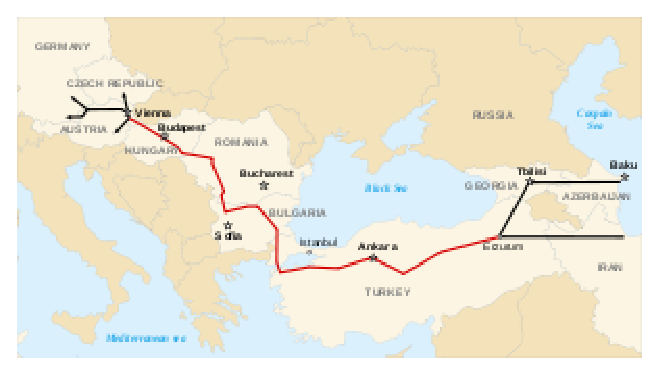
\epsfig{file=Nabucco.eps,height=\pos{4.5}{9}cm}
  \end{center}
    \caption{\brcolor{The Planned Nabucco Pipeline:}
    \pos{http://en.wikipedia.org/wiki/Nabucco\_Pipeline}{}}\label{pl.dia2} 
\end{figure}


\noindent
\begynd
\pind The Nabucco pipeline was, for many years, a planned pipeline
involving Austria, Turkey, Iran and other states and companies.
\afslut

\mnewfoil

\begin{figure}[ht]
  \begin{center}
  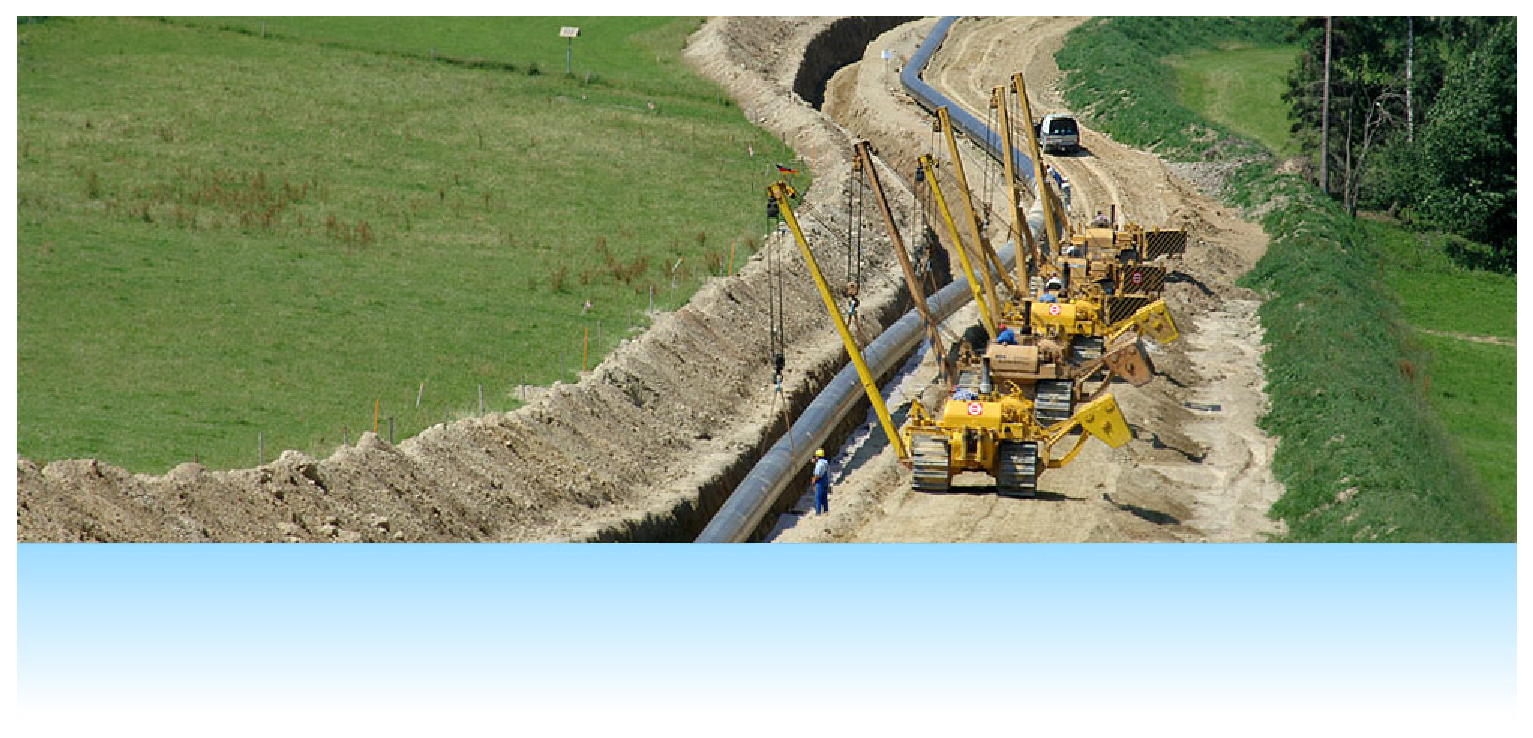
\epsfig{file=nabucco-digging,height=\pos{3.85}{11}cm}
  \end{center}
    \caption{\brcolor{Pipeline Construction}}\label{pl.dia3}
\end{figure}

\noindent
\begynd
\pind An example pipeline construction.
\pind It shows the linking of pipe segments.
\afslut
%\mnewfoil


\nbbbb{Pipes}

\begin{figure}[ht]
  \begin{center}
 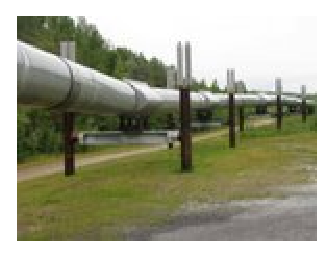
\epsfig{file=pipeline-1.eps,height=\pos{3.4}{6}cm}\ \ 
 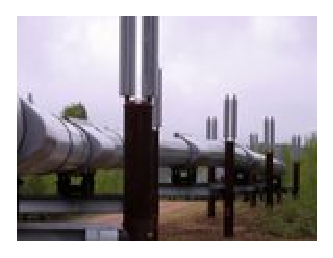
\epsfig{file=pipeline-2.eps,height=\pos{3.4}{6}cm}\ \ 
 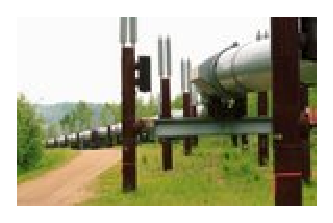
\epsfig{file=pipeline-3.eps,height=\pos{3.4}{6}cm}
  \end{center}
    \caption{\brcolor{Pipe Segments}}\label{pl.pipes}
 \end{figure}

\noindent
\begynd
\pind A pipe segment is a straight ``tube''-like unit.
\afslut
\nbbbb{Valves}
 
\begin{figure}[ht]
  \begin{center}
  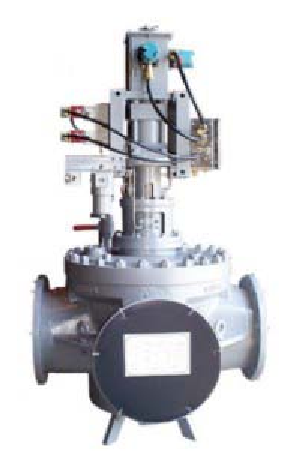
\epsfig{file=4Way-valve.eps,height=\pos{3.4}{6}cm}\ \ 
  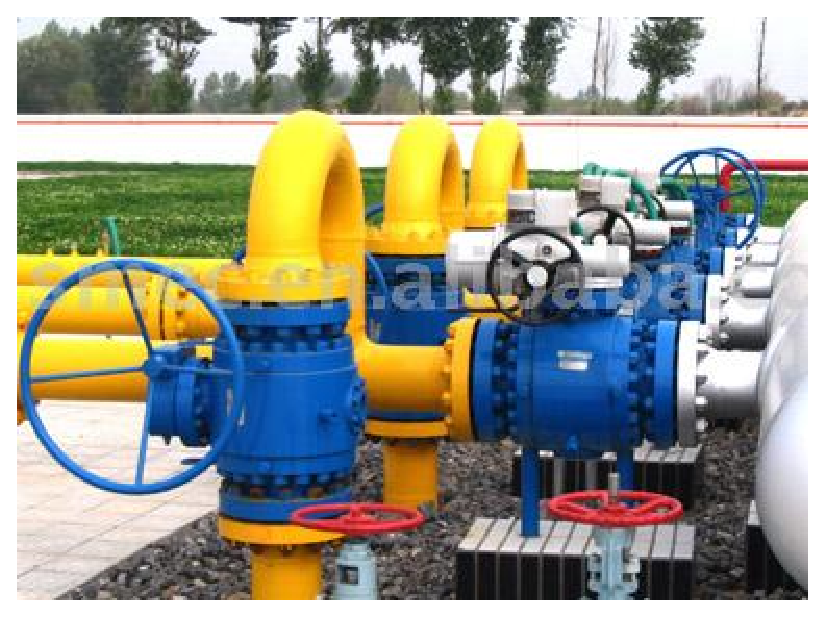
\epsfig{file=ball-valves.eps,height=\pos{3.4}{6}cm}\ \ 
  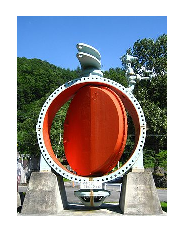
\epsfig{file=butterfly-valve-1.eps,height=\pos{3.4}{6}cm}\ \ 
  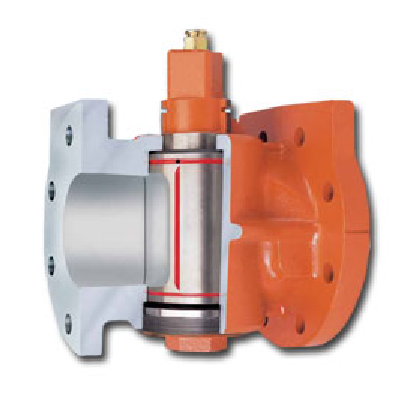
\epsfig{file=Resun-Plug-Valve.eps,height=\pos{3.4}{6}cm}
  \end{center}
    \caption{\brcolor{Valves}}\label{pl.valves}
 \end{figure}

\noindent
\begynd
\pind A pipe valve allows for the control of flow in pipes.
\afslut

\nbbbb{Pumps}
 
\begin{figure}[h]
  \begin{center}
      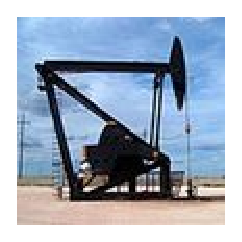
\epsfig{file=oil-drain-pump.eps,height=\pos{3.5}{7}cm}\ \ \ \ \
      \ \ \ \
      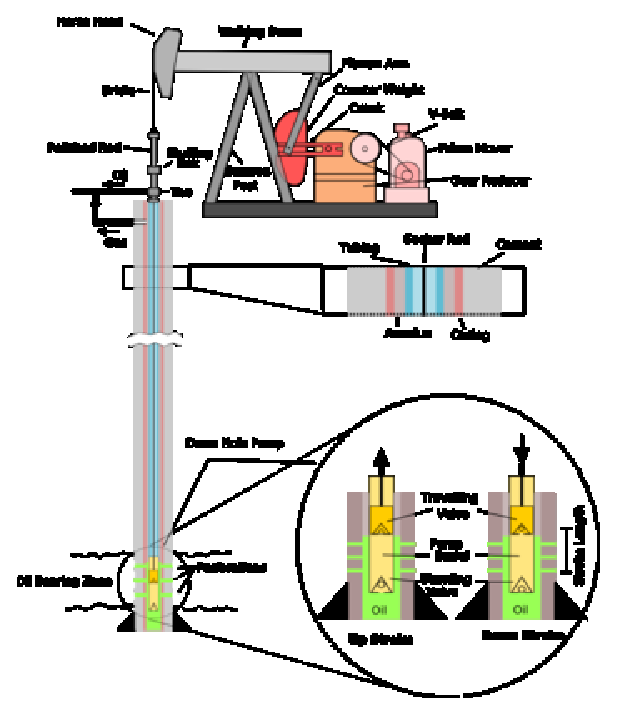
\epsfig{file=pump-jack.eps,height=\pos{3.5}{7}cm}
  \end{center}
    \caption{\brcolor{Oil Pumps}}\label{pl.pumps}
 \end{figure}

\noindent
\begynd
\pind A pump allows for the ``lifting'' of, for example, oil, over
      hilly terrain.
\pind The concept of \sfsl{pump head [height]} is relevant:
\begynd
\pind The \sfsl{head} is the height at which a pump can raise fluid up
      \nyl and is measured in meters or feet.
\afslut
\afslut

\nbbbb{Compressors}
 
\begin{figure}[h]
  \begin{center}
      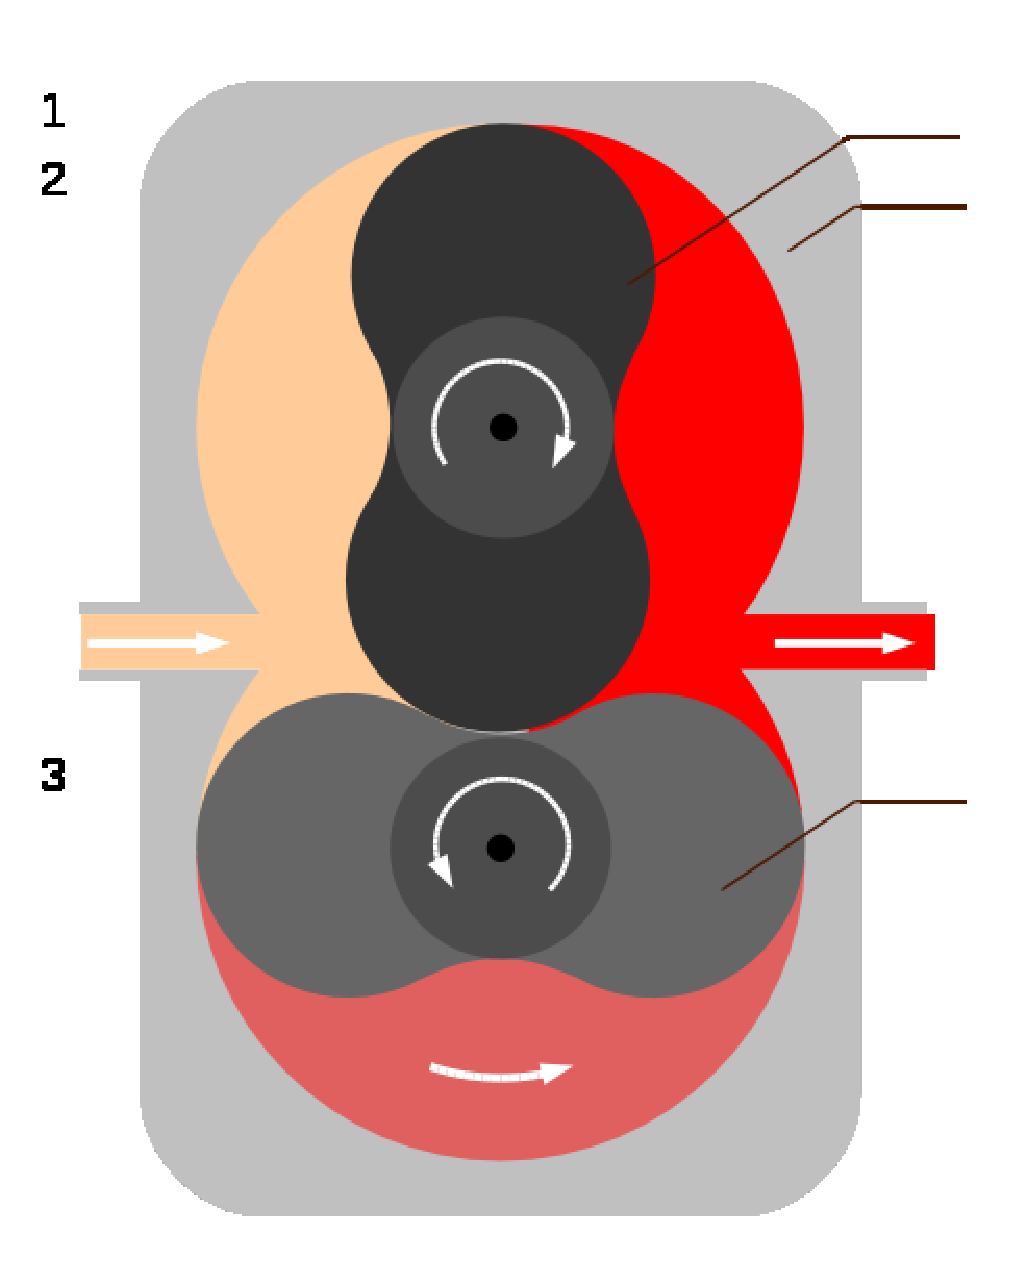
\epsfig{file=rotary-piston-pump.eps,height=\pos{3.4}{7}cm}\ \ \ 
      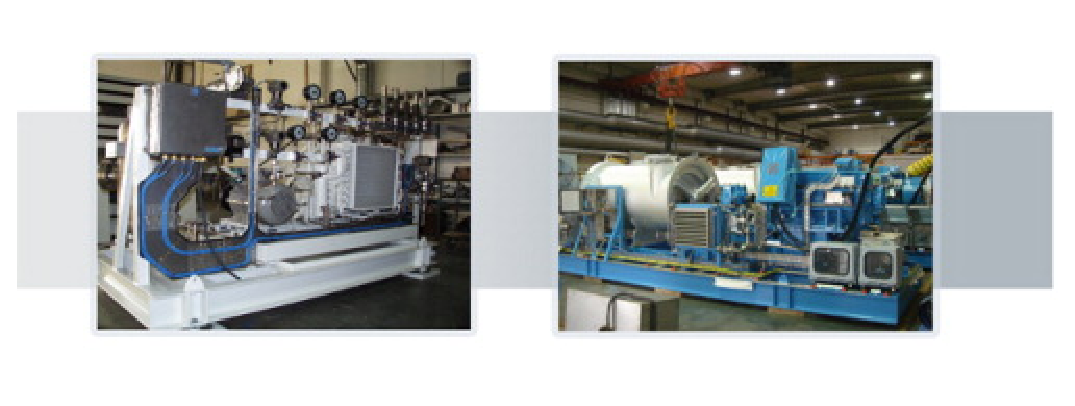
\epsfig{file=gas-compressor.eps,height=\pos{3.4}{7}cm}
  \end{center}
    \caption{\brcolor{Gas Compressors}}\label{pl.compressors}
 \end{figure}

\noindent
\begynd
\pind A compressor is used for gaseous liquids.
\begynd
\pind Compressors are similar to pumps: \nyl both increase the pressure on a fluid \nyl and both can transport the fluid through a pipe. \nyl As gases are compressible, \nyl the compressor also reduces the volume of a gas. 
\afslut
\afslut

\nbbbb{Pigs}
 
\begin{figure}[h]
  \begin{center}
  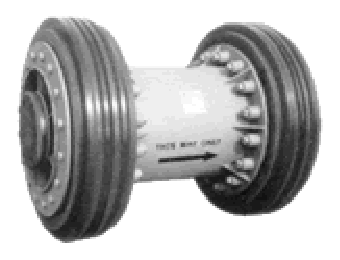
\epsfig{file=pig.eps,height=\pos{3.4}{7}cm}\ \ \ 
  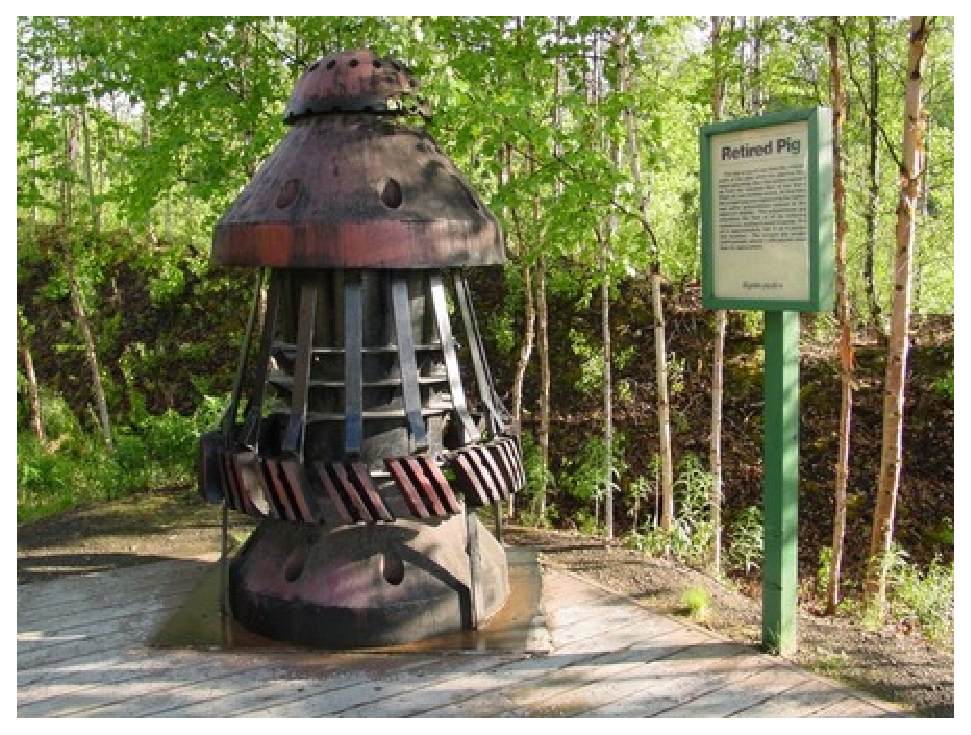
\epsfig{file=retired-pig.eps,height=\pos{3.4}{7}cm}
  \end{center}
    \caption{\brcolor{New and Old Pigs}}\label{pl.pig2} 
\end{figure}

\noindent
\begynd
\pind A ``pig'' is a tool that is sent down a pipeline and propelled
by the pressure of the product flow in the pipeline itself.  
\pind The primary purpose of pipeline pigs is to make sure that the
pipe is clean and free from obstruction.  
\afslut
\mnewfoil

\begin{figure}[h]
  \begin{center}
  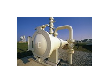
\epsfig{file=GasPigTrap.eps,height=\pos{3.4}{7}cm} \ \ 
  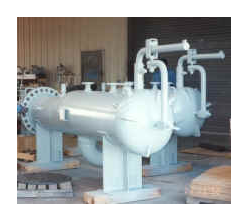
\epsfig{file=pig-receivers.eps,height=\pos{3.4}{7}cm}
  \end{center}
    \caption{\brcolor{Pig Launcher, Receiver}}\label{pl.pig1} 
 \end{figure}

\mnewfoil

\begin{figure}[ht]
  \begin{center}
    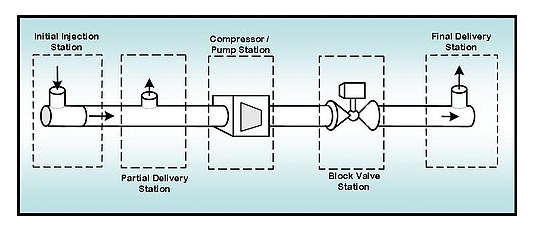
\epsfig{file=pipeline-diagram.eps,height=\pos{5}{8}cm}
    \caption{\brcolor{A Simple Pipeline}}\label{pi:pl.dia0}
  \end{center}
 \end{figure}

\noindent
\begynd
\pind Leftmost: A \sort{Well}. 
\pind 2nd from  left: a \sort{Fork}.
\pind Rightmost: a \sort{Sink}.
\afslut  
\mnewfoil

\begin{figure}[ht]
  \begin{center}
   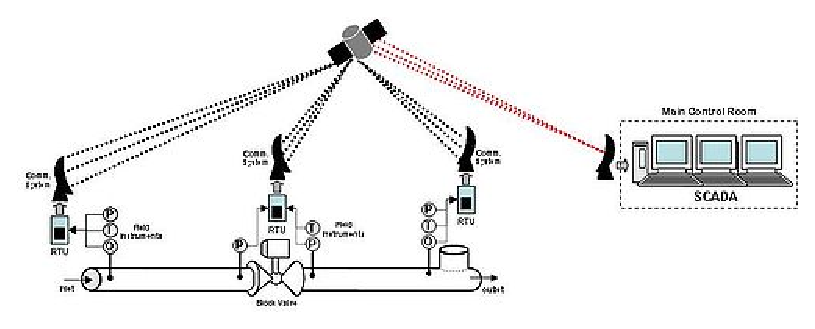
\epsfig{file=pipeline-scada.eps,height=\pos{5}{8}cm}
  \end{center}
    \caption{\brcolor{\LLLL\HHHH A Pipeline Monitoring \& Control System Diagram}}\label{pi:pl.dia1}
 \end{figure}

\noindent
\begynd
\pind Also called \sfsl{SCADA [Supervisory Control And Data Acquisition]}
\afslut 
%%  LocalWords:  Nabucco nd SCADA



\nbbbbb{Endurantes: Cualidades Externas}\label{pipe-ex1}\tehran{Endurants}{pipe:Edurants}\HHHH 

Seguimos la ontología de la Fig.\,\ref{anoipilisy}, el cuadro de líneas discontinuas de la izquierda
etiquetado como \sfsl{Cualidades Externas}.

\hDBfigure{onto}{\pos{10.8}{10}cm}{Ontología Superior}{anoipilisy}

\mnewfoil

\nbbbb{Partes}\tehran{Parts}{pipe:Parts}\HHHH

\DBfigure{opls-edin}{\pos{5}{10}cm}{Ejemplo de un sistema de tuberías}{nabucco}

\mnewfoil

\tehrantutorial{\begin{multicols}{2}}{}\HHHH
\begin{enumerate}\setei
\item \label{p-e-00} Un sistema de tuberías contiene un conjunto de unidades de tuberías y un monitor del sistema de tuberías.
\item \label{p-e--1} La buena formación de un sistema de tuberías
  depende de su mereología\pos{ (cf.\ sec.\,\ref{PLS Mereology})}{}
  y el enrutamiento de sus tuberías\pos{ (cf.\ sec.\,\ref{Wellformed Pipes})}{}. 
\item \label{p-e-01} Una unidad de tubería puede ser un pozo, una tubería, una bomba,
  una válvula, una bifurcación, una unión, una placa\footnote{\LLLL Una unidad de \sfsl{placa} es una
  placa de acero generalmente circular y plana utilizada para ``comenzar'' o ``terminar'' un
  segmento de tubería.}, o una unidad de desagüe.
\item \label{p-e-02} Consideramos todas estas unidades como
  distinguibles, es decir, el conjunto de pozos, el conjunto de tuberías, etc., el conjunto
  de desagües son disjuntos.
\savei\end{enumerate} 
\tehrantutorial{\end{multicols}}{}

\mnewfoil\LLLL
\tehrantutorial{\begin{multicols}{2}\footnotesize}{\LLLL}
\bp
\kw{type}\\
\ref{p-e-00}.\ \ PLS{\PRIM}, U, M \iptye{PLS$'$}{p-e-00}\iptye{U}{p-e-00}\iptye{M}{p-e-00}\\
\ref{p-e--1}.\ \ PLS {\EQ} {\LBRACE}{\BAR} pls:PLS{\PRIM}{\RDOT}wf\_PLS(pls) {\BAR}{\RBRACE} \iptye{PLS}{p-e--1} \\
\kw{value}\\
\ref{p-e--1}.\ \ wf\_PLS: PLS {\RIGHTARROW} \kw{Bool} \ipwf{wf\_PLS}{p-e--1}\\
\ref{p-e--1}.\ \ wf\_PLS(pls) {\IS}\\
\ref{p-e--1}.\ \ wf\_Mereology(pls){\WEDGE}wf\_Routes(pls){\WEDGE}wf\_Metrics(pls)\footnotemark\\
\ref{p-e-00}.\ \ obs\_Us: PLS {\RIGHTARROW} U\kw{-set} \ipob{obs\_Us}{p-e-00}\\
\ref{p-e-00}.\ \ obs\_M: PLS {\RIGHTARROW} M \ipob{obs\_M}{p-e-00}\\
\kw{type}\\
\ref{p-e-01}.\ \ U {\EQ} We {\BAR} Pi {\BAR} Pu {\BAR} Va {\BAR} Fo {\BAR} Jo {\BAR} Pl {\BAR} Si\iptye{U}{p-e-01}\\
\ref{p-e-02}.\ \ We :: Well\iptye{We}{p-e-02}\\
\ref{p-e-02}.\ \ Pi :: Pipe\iptye{Pi}{p-e-02} \\
\ref{p-e-02}.\ \ Pu :: Pump\iptye{Pu}{p-e-02} \\
\ref{p-e-02}.\ \ Va :: Valv\iptye{Va}{p-e-02}\\
\ref{p-e-02}.\ \ Fo :: Fork\iptye{Fo}{p-e-02}\\
\ref{p-e-02}.\ \ Jo :: Join\iptye{Jo}{p-e-02}\\
\ref{p-e-02}.\ \ Pl :: Plate\iptye{Pl}{p-e-02}\\
\ref{p-e-02}.\ \ Si :: Sink\iptye{Si}{p-e-02}
\ep
\tehrantutorial{\end{multicols}}{}
\footnotetext{\LLLL%
  \textsf{wf\_Mereology}, 
  \textsf{wf\_Routes} y
  \textsf{wf\_Metrics} se explicarán en las secciones\,%
  \vref{pipe:wfMereology},
  \vref{pipe:wfRoutes} y
  \vref{pipe:Wellformed Unit Metrics}.}


\nbbbb{Un Estado Endurante}

\begin{enumerate}\setei
\item \label{end-state-000} Para un sistema de tuberías dado % unsure how to make this flow well. The original english sentence is rather confusing.
\item \label{end-state-010} ejemplificamos un estado endurante $\sigma$
\item \label{end-state-020} compuesto del sistema de tuberías dado y
                            todas sus unidades manifiestas, es decir, sin placas.
\savei\end{enumerate}

\bp
\kw{value}\\
\ref{end-state-000}.\ \ \ pls:PLS\ \ \ipva{pls}{end-state-000}\\
\kw{variable}\\
\ref{end-state-010}.\ \ \ $\sigma$ :{\EQ} collect\_state(pls)\ \ \ipst{$\sigma$}{end-state-010} \\
\kw{value} \\
\ref{end-state-020}.\ \ \ collect\_state: PLS\ \ \ \ipfu{collect\_state}{end-state-020}\\
\ref{end-state-020}.\ \ \ collect\_state(pls) {\IS} {\LBRACE}pls{\RBRACE}\,{\UNION}\,obs\_Us(pls) {\SETMINUS} Pl
\ep

\nbbbbb{Endurantes: Cualidades Internas}

\begynd
\pind Seguimos la ontología de la fig.\,\vref{anoipilisy}, \nyl las
líneas verticales y horizontales de la izquierda.
\afslut


\bbbb{Identificación Única}

\begin{enumerate}\setei
\item \label{p-e-03z} El sistema de tuberías, como tal,
\item \label{p-e-03x} tiene un identificador único, distinto de sus
                      identificadores de unidades de tuberías. 
\item \label{p-e-03y} Cada unidad de tubería se distingue de manera única por
                      su identificador de unidad. 
\item \label{p-e-03zz} Existe un estado de todos los identificadores únicos.
\savei\end{enumerate}
\mnewfoil
%\RSLatex
%   type
%&\ref{p-e-03x}.&      PLSI &\iptyu{PLSI}{p-e-03x}&
%&\ref{p-e-03y}.&      UI &\iptyu{UI}{p-e-03y}&
%   value
%&\ref{p-e-03z}.&      pls:PLS
%&\ref{p-e-03x}.&      uid_PLS: PLS -> PLSI&\ipob{uid\_PLS}{p-e-03x}&
%&\ref{p-e-03y}.&      uid_U: U -> UI&\ipob{uid\_U}{p-e-03y}&
%   variable
%&\ref{p-e-03zz}.&      `sigma&$_{uid}$& := { uid_PLS(pls) } union xtr_UIs(pls) &\ipst{$\sigma_{uid}$}{p-e-03z}&
%   axiom &\ipax{Unique Identification}{p-e-03y}&
%&\ref{p-e-03y}.&      all u,u':U:-{u,u'}<<=obs_Us(pls)=>(u~=u'=>uid_UI(u)~=uid_UI(u'))
%&\ref{p-e-03y}.&    /\  uid_PLS(pls) ~isin {uid_UI(u)|u:U:-u isin obs_Us(pls)}
%\endRSLatex 
\bp
\>\ \kw{type}\\
\ref{p-e-03x}.\ \ \ \ \ \ PLSI \iptyu{PLSI}{p-e-03x}\\
\ref{p-e-03y}.\ \ \ \ \ \ UI \iptyu{UI}{p-e-03y}\\
\>\ \kw{value}\\
\ref{p-e-03z}.\ \ \ \ \ \ pls:PLS\\
\ref{p-e-03x}.\ \ \ \ \ \ uid\_PLS: PLS {\RIGHTARROW} PLSI\ipob{uid\_PLS}{p-e-03x}\\
\ref{p-e-03y}.\ \ \ \ \ \ uid\_U: U {\RIGHTARROW} UI\ipob{uid\_U}{p-e-03y}\\
\>\ \kw{variable}\\
\ref{p-e-03zz}.\ \ \ \ \ \ $\sigma$$_{uid}$ :{\EQ} {\LBRACE} uid\_PLS(pls) {\RBRACE} {\UNION} xtr\_UIs(pls) \ipst{$\sigma_{uid}$}{p-e-03z}\\
\>\ \kw{axiom} \ipax{Unique Identification}{p-e-03y}\\
\ref{p-e-03y}.\ \ \ \ \ \ {\ALL} u,u{\PRIM}:U{\RDOT}{\LBRACE}u,u{\PRIM}{\RBRACE}{\SUBSETEQ}obs\_Us(pls){\DBLRIGHTARROW}(u{\NOTEQ}u{\PRIM}{\DBLRIGHTARROW}uid\_UI(u){\NOTEQ}uid\_UI(u{\PRIM}))\\
\ref{p-e-03y}.\ \ \ \ {\WEDGE}\ \ uid\_PLS(pls) {\NOTISIN} {\LBRACE}uid\_UI(u){\BAR}u:U{\RDOT}u {\ISIN} obs\_Us(pls){\RBRACE}
\ep

\mnewfoil
\begin{enumerate}\setei
\item \label{p-e-03a} De un sistema de tuberías uno puede observar 
el conjunto de todos los identificadores únicos de unidades.
\savei\end{enumerate}


%\RSLatex
%   value
%&\ref{p-e-03a}.&   xtr_UIs: PLS -> UI-set&\ipfu{xtr\_UIs}{p-e-03a}&
%&\ref{p-e-03a}.&   xtr_UIs(pls) is {uid_UI(u)|u:U:-u isin obs_Us(pls)}
%\endRSLatex 
\bp
\>\ \kw{value}\\
\ref{p-e-03a}.\ \ \ xtr\_UIs: PLS {\RIGHTARROW} UI\kw{-set}\ipfu{xtr\_UIs}{p-e-03a}\\
\ref{p-e-03a}.\ \ \ xtr\_UIs(pls) {\IS} {\LBRACE}uid\_UI(u){\BAR}u:U{\RDOT}u {\ISIN} obs\_Us(pls){\RBRACE}
\ep

\begin{enumerate}\setei
\item \label{p-e-03b} Podemos demostrar que el número de identificadores
                      únicos de unidades es igual al número de unidades de ese sistema.
\savei\end{enumerate}


%\RSLatex
%   &\kw{theorem:}\ipth{Unique Endurants}{p-e-03b}&
%&\ref{p-e-03b}.&     all pls:PLS:-card obs_Us(pl)=card xtr_UIs(pls)
%\endRSLatex 
\bp
\>\ \kw{theorem:}\ipth{Endurantes Únicos}{p-e-03b}\\
\ref{p-e-03b}.\ \ \ \ \ {\ALL} pls:PLS{\RDOT}\kw{card} obs\_Us(pl){\EQ}\kw{card} xtr\_UIs(pls)
\ep

\nbbbb{Mereología}\label{PLS Mereology}\LLLL\HHHH

\bbb{Mereología PLS}

\item \label{pls-mer-00}La mereología de un sistema de tuberías es el 
  conjunto de identificadores únicos de todas las unidades del sistema.
\begin{enumerate}\setei
\savei\end{enumerate}

%\RSLatex
%type
%&\ref{pls-mer-00}.&   PLS_Mer = UI-set&\ipty{PLS\_Mer}{pls-mer-00}&
%value
%&\ref{pls-mer-00}.&   mereo_PLS: PLS -> PLS_Mer&\ipob{mereo\_PLS}{pls-mer-00}&
%axiom&\ipty{Wellformed Mereologies}{pls-mer-00}&
%&\ref{pls-mer-00}.&   all uis:PLS_Mer :- uis = card xtr_UIs(pls)
%\endRSLatex 
\bp
\kw{type}\\
\ref{pls-mer-00}.\ \ \ PLS\_Mer {\EQ} UI\kw{-set}\ipty{PLS\_Mer}{pls-mer-00}\\
\kw{value}\\
\ref{pls-mer-00}.\ \ \ mereo\_PLS: PLS {\RIGHTARROW} PLS\_Mer\ipob{mereo\_PLS}{pls-mer-00}\\
\kw{axiom}\ipty{Wellformed Mereologies}{pls-mer-00}\\
\ref{pls-mer-00}.\ \ \ {\ALL} uis:PLS\_Mer {\RDOT} uis {\EQ} \kw{card} xtr\_UIs(pls)
\ep

\nbbb{Unit Mereologies}\HHHH\LLLL

\begin{enumerate}\setei
\item \label{p-e-11}   Each unit is connected to zero, one or two
                       other existing input units and  zero, one or two
                       other existing output units as follows:
\begin{enumerate}
\item \label{p-e-04}   A well unit is connected to exactly one output
                       unit (and, hence, has no ``input'').
\item \label{p-e-05}   A pipe unit is connected to exactly one input unit
                       and one output unit.
\item \label{p-e-06}   A pump unit is connected to exactly one input unit
                       and one output unit.
\item \label{p-e-07}   A valve is connected to exactly one input unit
                       and one output unit.
\item \label{p-e-08}   A fork is connected to exactly one input unit
                       and two distinct output units.
\item \label{p-e-09}   A join is connected to exactly two distinct input units
                       and one output unit.
\item \label{p-e-85}   A plate is connected to exactly one unit.
\item \label{p-e-10}   A sink is connected to exactly one input unit
                       (and, hence, has no ``output''). 
\end{enumerate}
\savei\end{enumerate}

\mnewfoil\LLLL

%\RSLatex
%   type
%&\ref{p-e-11}.&      MER = UI-set >< UI-set&\iptym{MER}{p-e-11}&
%   value
%&\ref{p-e-11}.&      mereo_U: U -> MER &\ipob{mereo\_U}{p-e-11}&
%   axiom
%&\ref{p-e-11}.&       wf_Mereology: PLS -> Bool &\label{pipe:wfMereology}\ipwf{wf\_Mereology}{p-e-11}&
%&\ref{p-e-11}.&       wf_Mereology(pls) is
%&\ref{p-e-11}.&          all u:U:-u isin obs_Us(pls)=> 
%&\ref{p-e-11}.&             let (iuis,ouis) = mereo_U(u) in iuis union ouis <<= xtr_UIs(pls) /\
%&\ref{p-e-11}.&                 case (u,(card uius,card ouis)) of
%&\ref{p-e-04}.&                     (mk_We(we),(0,1)) -> true,
%&\ref{p-e-05}.&                     (mk_Pi(pi),(1,1)) -> true,
%&\ref{p-e-06}.&                     (mk_Pu(pu),(1,1)) -> true,
%&\ref{p-e-07}.&                     (mk_Va(va),(1,1)) -> true,
%&\ref{p-e-08}.&                     (mk_Fo(fo),(1,1)) -> true,
%&\ref{p-e-09}.&                     (mk_Jo(jo),(1,1)) -> true,
%&\ref{p-e-09}.&                     (mk_Pl(pl),(0,1)) -> true, &``begin''&
%&\ref{p-e-09}.&                     (mk_Pl(pl),(1,0)) -> true, &``end''&
%&\ref{p-e-10}.&                     (mk_Si(si),(1,1)) -> true,
%&\ref{p-e-11}.&                     _ -> false end end
%\endRSLatex 
\bp
\>\ \kw{type}\\
\ref{p-e-11}.\ \ \ \ \ \ MER {\EQ} UI\kw{-set} {\TIMES} UI\kw{-set}\iptym{MER}{p-e-11}\\
\>\ \kw{value}\\
\ref{p-e-11}.\ \ \ \ \ \ mereo\_U: U {\RIGHTARROW} MER \ipob{mereo\_U}{p-e-11}\\
\>\ \kw{axiom}\\
\ref{p-e-11}.\ \ \ \ \ \ \ wf\_Mereology: PLS {\RIGHTARROW} \kw{Bool} \label{pipe:wfMereology}\ipwf{wf\_Mereology}{p-e-11}\\
\ref{p-e-11}.\ \ \ \ \ \ \ wf\_Mereology(pls) {\IS}\\
\ref{p-e-11}.\ \ \ \ \ \ \ \ \ \ {\ALL} u:U{\RDOT}u {\ISIN} obs\_Us(pls){\DBLRIGHTARROW} \\
\ref{p-e-11}.\ \ \ \ \ \ \ \ \ \ \ \ \ \kw{let} (iuis,ouis) {\EQ} mereo\_U(u) \kw{in} iuis {\UNION} ouis {\SUBSETEQ} xtr\_UIs(pls) {\WEDGE}\\
\ref{p-e-11}.\ \ \ \ \ \ \ \ \ \ \ \ \ \ \ \ \ \kw{case} (u,(\kw{card} uius,\kw{card} ouis)) \kw{of}\\
\ref{p-e-04}.\ \ \ \ \ \ \ \ \ \ \ \ \ \ \ \ \ \ \ \ \ (mk\_We(we),(0,1)) {\RIGHTARROW} \kw{true},\\
\ref{p-e-05}.\ \ \ \ \ \ \ \ \ \ \ \ \ \ \ \ \ \ \ \ \ (mk\_Pi(pi),(1,1)) {\RIGHTARROW} \kw{true},\\
\ref{p-e-06}.\ \ \ \ \ \ \ \ \ \ \ \ \ \ \ \ \ \ \ \ \ (mk\_Pu(pu),(1,1)) {\RIGHTARROW} \kw{true},\\
\ref{p-e-07}.\ \ \ \ \ \ \ \ \ \ \ \ \ \ \ \ \ \ \ \ \ (mk\_Va(va),(1,1)) {\RIGHTARROW} \kw{true},\\
\ref{p-e-08}.\ \ \ \ \ \ \ \ \ \ \ \ \ \ \ \ \ \ \ \ \ (mk\_Fo(fo),(1,1)) {\RIGHTARROW} \kw{true},\\
\ref{p-e-09}.\ \ \ \ \ \ \ \ \ \ \ \ \ \ \ \ \ \ \ \ \ (mk\_Jo(jo),(1,1)) {\RIGHTARROW} \kw{true},\\
\ref{p-e-09}.\ \ \ \ \ \ \ \ \ \ \ \ \ \ \ \ \ \ \ \ \ (mk\_Pl(pl),(0,1)) {\RIGHTARROW} \kw{true}, ``begin''\\
\ref{p-e-09}.\ \ \ \ \ \ \ \ \ \ \ \ \ \ \ \ \ \ \ \ \ (mk\_Pl(pl),(1,0)) {\RIGHTARROW} \kw{true}, ``end''\\
\ref{p-e-10}.\ \ \ \ \ \ \ \ \ \ \ \ \ \ \ \ \ \ \ \ \ (mk\_Si(si),(1,1)) {\RIGHTARROW} \kw{true},\\
\ref{p-e-11}.\ \ \ \ \ \ \ \ \ \ \ \ \ \ \ \ \ \ \ \ \ {\UNDERLINE} {\RIGHTARROW} \kw{false} \kw{end} \kw{end}
\ep

\nbbbb{Pipeline Concepts, I}

\bbb{Pipe Routes}\label{primer-pipe}\HHHH

\begin{enumerate}\setei
\item \label{p-e-12} A route (of a pipeline system) is a sequence of
                     connected units (of the pipeline system). 
\item \label{p-e-13} A route descriptor is a sequence of unit
                     identifiers and the connected units of a route
                     (of a pipeline system).
\savei\end{enumerate}

%\RSLatex
%   type
%&\ref{p-e-12}.&      R' = U-inflist &\iptyo{R$'$}{p-e-12}&
%&\ref{p-e-12}.&      R = {| r:Route':-wf_Route(r) |} &\iptyo{R}{p-e-12}&
%&\ref{p-e-13}.&      RD = UI-inflist &\iptyo{RD}{p-e-13}&
%   axiom
%&\ref{p-e-13}.&      all rd:RD :- exists r:R:-rd=descriptor(r) &\ipax{Route Describability}{p-e-13}&
%   value
%&\ref{p-e-13}.&      descriptor: R -> RD &\ipfu{descriptor}{p-e-13}&
%&\ref{p-e-13}.&      descriptor(r) is <.uid_UI(r[i])|i:Nat:-1<=i<=len r.>   
%\endRSLatex 
\bp
\>\ \kw{type}\\
\ref{p-e-12}.\ \ \ \ \ \ R{\PRIM} {\EQ} U$^{\omega}$ \iptyo{R$'$}{p-e-12}\\
\ref{p-e-12}.\ \ \ \ \ \ R {\EQ} {\LBRACE}{\BAR} r:Route{\PRIM}{\RDOT}wf\_Route(r) {\BAR}{\RBRACE} \iptyo{R}{p-e-12}\\
\ref{p-e-13}.\ \ \ \ \ \ RD {\EQ} UI$^{\omega}$ \iptyo{RD}{p-e-13}\\
\>\ \kw{axiom}\\
\ref{p-e-13}.\ \ \ \ \ \ {\ALL} rd:RD {\RDOT} {\EXISTS} r:R{\RDOT}rd{\EQ}descriptor(r) \ipax{Route Describability}{p-e-13}\\
\>\ \kw{value}\\
\ref{p-e-13}.\ \ \ \ \ \ descriptor: R {\RIGHTARROW} RD \ipfu{descriptor}{p-e-13}\\
\ref{p-e-13}.\ \ \ \ \ \ descriptor(r) {\IS} {\LANGLE}uid\_UI(r{\LBRACKET}i{\RBRACKET}){\BAR}i:\kw{Nat}{\RDOT}1{\LEQ}i{\LEQ}\kw{len} r{\RANGLE}\ \ \ 
\ep

\mnewfoil\LLLL\HHHH

\begin{enumerate}\setei
\item \label{p-e-20x}   Two units are adjacent if the output unit
  identifiers of one shares a unique unit identifier with the input
  identifiers of the other.
\savei\end{enumerate}

%\RSLatex
%   value 
%&\ref{p-e-20x}.&      adjacent: U >< U -> Bool &\ipfu{adjacent}{p-e-20x}&
%&\ref{p-e-20x}.&      adjacent(u,u') is let (,ouis)=mereo_U(u),(iuis,)=mereo_U(u') in ouis inter iuis ~= {} end
%\endRSLatex 
\bp
\>\ \kw{value} \\
\ref{p-e-20x}.\ \ \ \ \ \ adjacent: U {\TIMES} U {\RIGHTARROW} \kw{Bool} \ipfu{adjacent}{p-e-20x}\\
\ref{p-e-20x}.\ \ \ \ \ \ adjacent(u,u{\PRIM}) {\IS} \kw{let} (,ouis){\EQ}mereo\_U(u),(iuis,){\EQ}mereo\_U(u{\PRIM}) \kw{in} ouis {\INTER} iuis {\NOTEQ} {\LBRACE}{\RBRACE} \kw{end}
\ep

\LLLL

\begin{enumerate}\setei
\item \label{p-e-20a}   Given a pipeline system, $pls$, one can identify the
                  (possibly infinite) set of (possibly infinite) routes
                  of that pipeline system.
\begin{enumerate}
\item \label{p-e-20}  The empty sequence, {\LANGLE}{\RANGLE}, is a
                      route of $pls$.  
\item \label{p-e-21}  Let $u, u'$ be any units of $pls$, such that
                      an output unit identifier of $u$ is the same as
                      an input unit identifier of $u'$ then
                      {\LANGLE}$u,u'${\RANGLE} is a route of $pls$.
\item \label{p-e-22}  If $r$ and $r'$ are routes of $pls$ such that
                      the last element of $r$ is the same as the first
                      element of $r'$, then $r${\CONCAT}\kw{tl}$r'$ is
                      a route of $pls$.  
\item \label{p-e-23}  No sequence of units is a route unless it
                      follows from a finite (or an infinite) number of
                      applications of the basis and induction clauses
                      of Items~\ref{p-e-20}--\ref{p-e-22}.
\end{enumerate}
\savei\end{enumerate}

\mnewfoil\LLLL\HHHH

%\RSLatex 
%   value
%&\ref{p-e-20a}.&      Routes: PLS -> RD-infset&\ipfu{Routes}{p-e-20a}&
%&\ref{p-e-20a}.&      Routes(pls) is 
%&\ref{p-e-20}.&          let rs = <..> union 
%&\ref{p-e-21}.&                   {<.uid_UI(u),uid_UI(u').>|u,u':U:-{u,u'}<<=obs_Us(pls) /\ adjacent(u,u')}
%&\ref{p-e-22}.&                 union {r^tl r'|r,r':R:-{r,r'}<<=rs}
%&\ref{p-e-23}.&          in rs end
%\endRSLatex 
\bp
\>\ \kw{value}\\
\ref{p-e-20a}.\ \ \ \ \ \ Routes: PLS {\RIGHTARROW} RD\kw{-infset}\ipfu{Routes}{p-e-20a}\\
\ref{p-e-20a}.\ \ \ \ \ \ Routes(pls) {\IS} \\
\ref{p-e-20}.\ \ \ \ \ \ \ \ \ \ \kw{let} rs {\EQ} {\LANGLE}{\RANGLE} {\UNION} \\
\ref{p-e-21}.\ \ \ \ \ \ \ \ \ \ \ \ \ \ \ \ \ \ \ {\LBRACE}{\LANGLE}uid\_UI(u),uid\_UI(u{\PRIM}){\RANGLE}{\BAR}u,u{\PRIM}:U{\RDOT}{\LBRACE}u,u{\PRIM}{\RBRACE}{\SUBSETEQ}obs\_Us(pls) {\WEDGE} adjacent(u,u{\PRIM}){\RBRACE}\\
\ref{p-e-22}.\ \ \ \ \ \ \ \ \ \ \ \ \ \ \ \ \ {\UNION} {\LBRACE}r{\CONCAT}\kw{tl} r{\PRIM}{\BAR}r,r{\PRIM}:R{\RDOT}{\LBRACE}r,r{\PRIM}{\RBRACE}{\SUBSETEQ}rs{\RBRACE}\\
\ref{p-e-23}.\ \ \ \ \ \ \ \ \ \ \kw{in} rs \kw{end}
\ep

\bbb{Well-formed Routes}\label{Wellformed Pipes}

\begin{enumerate}\setei
\item \label{p-e-14a}  A route is acyclic if no two route positions
  reveal the same unique unit identifier.
\savei\end{enumerate}
%\RSLatex
%   value
%&\ref{p-e-14a}.&   is_acyclic_Route: R -> Bool&\ippr{is\_acyclic\_Route}{p-e-14a}&
%&\ref{p-e-14a}.&   is_acyclic_Route(r) is ~exists i,j:Nat:-{i,j}<<=inds r /\ i~=j /\ r[i]=r[j]
%\endRSLatex 
\bp
\>\ \kw{value}\\
\ref{p-e-14a}.\ \ \ is\_acyclic\_Route: R {\RIGHTARROW} \kw{Bool}\ippr{is\_acyclic\_Route}{p-e-14a}\\
\ref{p-e-14a}.\ \ \ is\_acyclic\_Route(r) {\IS} {\SIM}{\EXISTS} i,j:\kw{Nat}{\RDOT}{\LBRACE}i,j{\RBRACE}{\SUBSETEQ}\kw{inds} r {\WEDGE} i{\NOTEQ}j {\WEDGE} r{\LBRACKET}i{\RBRACKET}{\EQ}r{\LBRACKET}j{\RBRACKET}
\ep

\mnewfoil

\begin{enumerate}\setei
\item \label{p-e-14b}  A pipeline system is well-formed if none of its
                      routes are circular (and all of its routes
                      embedded in well-to-sink routes). 
\savei\end{enumerate}
%\RSLatex
%   value
%&\ref{p-e-14b}.&   wf_Routes: PLS -> Bool&\ipwf{wf\_Routes}{p-e-14b}&
%&\ref{p-e-14b}.&   wf_Routes(pls) is  &\label{pipe:wfRoutes}&
%&\ref{p-e-14b}.&       non_circular(pls) /\ are_embedded_Routes(pls)
%
%&\ref{p-e-14b}.&   is_non_circular_PLS: PLS -> Bool&\ipwf{is\_non\_circular\_PLS}{p-e-14b}&
%&\ref{p-e-14b}.&   is_non_circular_PLS(pls) is 
%&\ref{p-e-14b}.&       all r:R:-r isin routes(p)/\acyclic_Route(r)
%\endRSLatex 
\bp
\>\ \kw{value}\\
\ref{p-e-14b}.\ \ \ wf\_Routes: PLS {\RIGHTARROW} \kw{Bool}\ipwf{wf\_Routes}{p-e-14b}\\
\ref{p-e-14b}.\ \ \ wf\_Routes(pls) {\IS}\ \ \label{pipe:wfRoutes}\\
\ref{p-e-14b}.\ \ \ \ \ \ \ non\_circular(pls) {\WEDGE} are\_embedded\_Routes(pls)\\
\\
\ref{p-e-14b}.\ \ \ is\_non\_circular\_PLS: PLS {\RIGHTARROW} \kw{Bool}\ipwf{is\_non\_circular\_PLS}{p-e-14b}\\
\ref{p-e-14b}.\ \ \ is\_non\_circular\_PLS(pls) {\IS} \\
\ref{p-e-14b}.\ \ \ \ \ \ \ {\ALL} r:R{\RDOT}r {\ISIN} routes(p){\WEDGE}acyclic\_Route(r)
\ep

\mnewfoil

\begin{enumerate}\setei
\item \label{p-e-19}  We define well-formedness in terms of
  well-to-sink routes, i.e., routes which start with a well unit and
  end with a sink unit.
\savei\end{enumerate}

%\RSLatex
%   value   
%&\ref{p-e-19}.&   well_to_sink_Routes: PLS -> R-set&\ipfu{well\_to\_sink\_Routes}{p-e-19}&
%&\ref{p-e-19}.&   well_to_sink_Routes(pls) is
%&\ref{p-e-19}.&      let rs = Routes(pls) in
%&\ref{p-e-19}.&      {r|r:R:-r isin rs /\ is_We(r[1]) /\ is_Si(r[len r])} end
%\endRSLatex 
\bp
\>\ \kw{value}\ \ \ \\
\ref{p-e-19}.\ \ \ well\_to\_sink\_Routes: PLS {\RIGHTARROW} R\kw{-set}\ipfu{well\_to\_sink\_Routes}{p-e-19}\\
\ref{p-e-19}.\ \ \ well\_to\_sink\_Routes(pls) {\IS}\\
\ref{p-e-19}.\ \ \ \ \ \ \kw{let} rs {\EQ} Routes(pls) \kw{in}\\
\ref{p-e-19}.\ \ \ \ \ \ {\LBRACE}r{\BAR}r:R{\RDOT}r {\ISIN} rs {\WEDGE} is\_We(r{\LBRACKET}1{\RBRACKET}) {\WEDGE} is\_Si(r{\LBRACKET}\kw{len} r{\RBRACKET}){\RBRACE} \kw{end}
\ep

\mnewfoil

\begin{enumerate}\setei
\item \label{p-e-18} A pipeline system is well-formed
      if all of its routes are embedded in well-to-sink routes.
\savei\end{enumerate}

%\RSLatex
%&\ref{p-e-18}.&   are_embedded_Routes: PLS -> Bool&\ippr{are\_embedded\_Routes}{p-e-18}&
%&\ref{p-e-18}.&   are_embedded_Routes(pls) is   
%&\ref{p-e-18}.&       let wsrs = well_to_sink_Routes(pls) in
%&\ref{p-e-18}.&       all r:R :- r isin Routes(pls) =>
%&\ref{p-e-18}.&           exists r':R,i,j:Nat :- 
%&\ref{p-e-18}.&              r' isin wsrs /\ {i,j}<<=inds r'/\i<=j /\ r = <.r'[k]|k:Nat:-i<=k<=j.> end
%\endRSLatex 
\bp
\ref{p-e-18}.\ \ \ are\_embedded\_Routes: PLS {\RIGHTARROW} \kw{Bool}\ippr{are\_embedded\_Routes}{p-e-18}\\
\ref{p-e-18}.\ \ \ are\_embedded\_Routes(pls) {\IS}\ \ \ \\
\ref{p-e-18}.\ \ \ \ \ \ \ \kw{let} wsrs {\EQ} well\_to\_sink\_Routes(pls) \kw{in}\\
\ref{p-e-18}.\ \ \ \ \ \ \ {\ALL} r:R {\RDOT} r {\ISIN} Routes(pls) {\DBLRIGHTARROW}\\
\ref{p-e-18}.\ \ \ \ \ \ \ \ \ \ \ {\EXISTS} r{\PRIM}:R,i,j:\kw{Nat} {\RDOT} \\
\ref{p-e-18}.\ \ \ \ \ \ \ \ \ \ \ \ \ \ r{\PRIM} {\ISIN} wsrs {\WEDGE} {\LBRACE}i,j{\RBRACE}{\SUBSETEQ}\kw{inds} r{\PRIM}{\WEDGE}i{\LEQ}j {\WEDGE} r {\EQ} {\LANGLE}r{\PRIM}{\LBRACKET}k{\RBRACKET}{\BAR}k:\kw{Nat}{\RDOT}i{\LEQ}k{\LEQ}j{\RANGLE} \kw{end}
\ep

\bbb{Embedded Routes}

\begin{enumerate}\setei
\item \label{p-e-33a} For every route we can define the set of all its
                      embedded routes. 
\savei\end{enumerate} 

%\RSLatex
%   value
%&\ref{p-e-33a}.&  embedded_Routes: R -> R-set&\ipfu{embedded\_Routes}{p-e-33a}&
%&\ref{p-e-33a}.&  embedded_Routes(r) is {<.r[k]|k:Nat:-i<=k<=j.> | i,j:Nat:- i {i,j}<<=inds(r) /\ i<=j}  
%\endRSLatex 
\bp
\>\ \kw{value}\\
\ref{p-e-33a}.\ \ embedded\_Routes: R {\RIGHTARROW} R\kw{-set}\ipfu{embedded\_Routes}{p-e-33a}\\
\ref{p-e-33a}.\ \ embedded\_Routes(r) {\IS} {\LBRACE}{\LANGLE}r{\LBRACKET}k{\RBRACKET}{\BAR}k:\kw{Nat}{\RDOT}i{\LEQ}k{\LEQ}j{\RANGLE} {\BAR} i,j:\kw{Nat}{\RDOT} i {\LBRACE}i,j{\RBRACE}{\SUBSETEQ}\kw{inds}(r) {\WEDGE} i{\LEQ}j{\RBRACE}\ \ 
\ep

\nbbb{A Theorem}

\begin{enumerate}\setei
\item \label{p-e-33b} The following theorem is conjectured:
\begin{enumerate}
\item \label{p-e-30}  the set of all routes  (of the pipeline system)
\item \label{p-e-31}  is the set of all well-to-sink routes (of a
                      pipeline system) and 
\item \label{p-e-32}  all their embedded routes
\end{enumerate}
\savei\end{enumerate}

%\RSLatex
%   &\kw{theorem:}\ipth{Routes of a PLS}{p-e-33b}&
%&\ref{p-e-33b}.&   all pls:PLS :-
%&\ref{p-e-33b}.&   let rs = Routes(pls),
%&\ref{p-e-33b}.&       wsrs = well_to_sink_Routes(pls) in
%&\ref{p-e-30}.&   rs = 
%&\ref{p-e-31}.&        wsrs union
%&\ref{p-e-32}.&        union {{r'|r':R :- r' isin is_embedded_Routes(r'')} | r'':R :- r'' isin wsrs}
%&\ref{p-e-33a}.&   end
%\endRSLatex 
\bp
\>\ \kw{theorem:}\ipth{Routes of a PLS}{p-e-33b}\\
\ref{p-e-33b}.\ \ \ {\ALL} pls:PLS {\RDOT}\\
\ref{p-e-33b}.\ \ \ \kw{let} rs {\EQ} Routes(pls),\\
\ref{p-e-33b}.\ \ \ \ \ \ \ wsrs {\EQ} well\_to\_sink\_Routes(pls) \kw{in}\\
\ref{p-e-30}.\ \ \ rs {\EQ} \\
\ref{p-e-31}.\ \ \ \ \ \ \ \ wsrs {\UNION}\\
\ref{p-e-32}.\ \ \ \ \ \ \ \ {\UNION} {\LBRACE}{\LBRACE}r{\PRIM}{\BAR}r{\PRIM}:R {\RDOT} r{\PRIM} {\ISIN} is\_embedded\_Routes(r{\PRIM}{\PRIM}){\RBRACE} {\BAR} r{\PRIM}{\PRIM}:R {\RDOT} r{\PRIM}{\PRIM} {\ISIN} wsrs{\RBRACE}\\
\ref{p-e-33a}.\ \ \ \kw{end}
\ep

\nbbb{Fluids}

\begin{enumerate}\setei
\item \label{p-e-34} The only fluid of concern to pipelines is the
                     gas\footnote{\LLLL Gaseous materials include: air, gas,
                     etc.} or liquid\footnote{\LLLL Liquid materials include
                     water, oil, etc.} which the pipes
                     transport\footnote{\LLLL The description of this
                     document is relevant only to gas or oil pipelines.}.
\savei\end{enumerate}

%\RSLatex
%   type
%&\ref{p-e-34}.&      GoL [ = M ] &\iptye{GoL}{p-e-34}&
%   value
%&\ref{p-e-34}.&      obs_GoL: U -> GoL&\ipob{obs\_GoL}{p-e-34}&  
%\endRSLatex 
\bp
\>\ \kw{type}\\
\ref{p-e-34}.\ \ \ \ \ \ GoL {\LBRACKET} {\EQ} M {\RBRACKET} \iptye{GoL}{p-e-34}\\
\>\ \kw{value}\\
\ref{p-e-34}.\ \ \ \ \ \ obs\_GoL: U {\RIGHTARROW} GoL\ipob{obs\_GoL}{p-e-34}\ \ 
\ep

\nbbbb{Attributes}\LLLL

\bbb{Unit Flow Attributes}\HHHH


\begin{enumerate}\setei
\item A number of attribute types characterise units:
\begin{enumerate}
\item \label{pa01x} estimated current well capacity (barrels of oil, etc.),
\item \label{pa03x} pump height (a static attribute), 
\item \label{pa04x} current pump status (not pumping, pumping; a programmable attribute),
\item \label{pa05x} current valve status (closed, open; a programmable attribute) and
\item \label{pa06x} flow (barrels/second, a biddable attribute).
\end{enumerate}
\savei\end{enumerate}

\mnewfoil\LLLL\HHHH%&$_{\mathcall{L}}$&

%\begin{multicols}{2}
%\RSLatex
%   type
%&\ref{pa01x}.&      WellCap &\iptya{WellCap}{pa01x}&
%&\ref{pa03x}.&      Pump_Height &\iptya{Pump\_Height}{pa03x}&
%&\ref{pa04x}.&      Pump_State == {|&\sort{not\_pumping}&,&\sort{pumping}&|} &\iptya{Pump\_State}{pa04x}&
%&\ref{pa05x}.&      Valve_State == {|&\sort{closed}&,&\sort{open}&|} &\iptya{Valve\_State}{pa05x}&
%&\ref{pa06x}.&      Flow &\iptya{Flow}{pa06x}&
%\endRSLatex 
\bp
\>\ \kw{type}\\
\ref{pa01x}.\ \ \ \ \ \ WellCap \iptya{WellCap}{pa01x}\\
\ref{pa03x}.\ \ \ \ \ \ Pump\_Height \iptya{Pump\_Height}{pa03x}\\
\ref{pa04x}.\ \ \ \ \ \ Pump\_State {\EQ}{\EQ} {\LBRACE}{\BAR}\sort{not\_pumping},\sort{pumping}{\BAR}{\RBRACE} \iptya{Pump\_State}{pa04x}\\
\ref{pa05x}.\ \ \ \ \ \ Valve\_State {\EQ}{\EQ} {\LBRACE}{\BAR}\sort{closed},\sort{open}{\BAR}{\RBRACE} \iptya{Valve\_State}{pa05x}\\
\ref{pa06x}.\ \ \ \ \ \ Flow \iptya{Flow}{pa06x}
\ep
\begin{enumerate}\setei
\item \label{pa05y1} Flows can be added and subtracted,
\item \label{pa05y2} added distributively  and
\item \label{pa05z} flows can be compared.
\savei\end{enumerate}

%\RSLatex
%   value
%&\ref{pa05y1}.&      &$\oplus,\ominus$&: Flow><Flow -> Flow &\ipop{$\oplus$}{pa05y1}\ipop{$\ominus$}{pa05y1}&
%&\ref{pa05y2}.&      &$\oplus$&: Flow-set -> Flow  &\ipop{$\oplus$}{pa05y2}&
%&\ref{pa05z}.&      <,<=,=,~=,>=,>: Flow >< Flow -> Bool
%\endRSLatex 
\bp
\>\ \kw{value}\\
\ref{pa05y1}.\ \ \ \ \ \ $\oplus,\ominus$: Flow{\TIMES}Flow {\RIGHTARROW} Flow \ipop{$\oplus$}{pa05y1}\ipop{$\ominus$}{pa05y1}\\
\ref{pa05y2}.\ \ \ \ \ \ $\oplus$: Flow\kw{-set} {\RIGHTARROW} Flow\ \ \ipop{$\oplus$}{pa05y2}\\
\ref{pa05z}.\ \ \ \ \ \ {\LT},{\LEQ},{\EQ},{\NOTEQ},{\GEQ},{\GT}: Flow {\TIMES} Flow {\RIGHTARROW} \kw{Bool}
\ep
\ipop{\LT}{pa05z}%
\ipop{\LEQ}{pa05z}%
\ipop{\EQ}{pa05z}%
\ipop{\NOTEQ}{pa05z}%
\ipop{\GEQ}{pa05z}%
\ipop{\GT}{pa05z}
\mnewfoil
\begin{enumerate}\setei
\item \label{pa00} Properties of pipeline units include
%%%\begin{multicols}{2}
\begin{enumerate}
\item \label{pa01} estimated current well capacity (barrels of oil,
  etc.) [a biddable attribute], 
\item \label{pa02} pipe length [a static attribute],
\item \label{pa03} current pump height [a biddable attribute], 
\item \label{pa04} current valve open/close status [a programmable attribute],
\item \label{pa05} current [$\mathcal{L}$aminar] in-flow at unit input
                   [a monitorable attribute],
\item \label{pa06} current $\mathcal{L}$aminar] in-flow leak at unit input
                   [a monitorable attribute],
\item \label{pa07} maximum [$\mathcal{L}$aminar] guaranteed in-flow leak at unit input
  [a static attribute],
\mnewfoil
\item \label{pa08} current [$\mathcal{L}$aminar] leak unit interior
                   [a monitorable attribute],
\item \label{pa09} current [$\mathcal{L}$aminar] flow in unit interior
                   [a monitorable attribute],
\item \label{pa10} maximum $\mathcal{L}$aminar] guaranteed flow in unit interior
                   [a monitorable attribute],
\item \label{pa11} current [$\mathcal{L}$aminar] out-flow at unit output
                   [a monitorable attribute],
\item \label{pa12} current [$\mathcal{L}$aminar] out-flow leak at unit output
                   [a monitorable attribute] and
\item \label{pa13} maximum guaranteed $\mathcal{L}$aminar out-flow leak at unit output
                   [a static attribute.
\end{enumerate}
%%%\end{multicols}
\savei\end{enumerate}
\mnewfoil
\begin{multicols}{2}\LLLL
%\RSLatex
%type 
%&\ref{pa05}&  In_Flow = Flow&\iptya{In\_Flow}{pa05}&
%&\ref{pa06}&  In_Leak = Flow&\iptya{In\_Leak}{pa06}&
%&\ref{pa07}&  Max_In_Leak = Flow&\iptya{Max\_In\_Leak}{pa07}&
%&\ref{pa08}&  Body_Flow = Flow&\iptya{Body\_Flow}{pa08}&
%&\ref{pa09}&   Body_Leak = Flow&\iptya{Body\_Leak}{pa09}&
%&\ref{pa10}&   Max_Flow = Flow&\iptya{Max\_Flow}{pa10}&
%&\ref{pa11}&  Out_Flow = Flow&\iptya{Out\_Flow}{pa11}&
%&\ref{pa12}&   Out_Leak = Flow&\iptya{Out\_Leak}{pa12}& 
%&\ref{pa13}&  Max_Out_Leak = Flow&\iptya{Max\_Out\_Leak}{pa13}&
%value
%&\ref{pa01}&  attr_WellCap: We -> WellCap    
%&\ref{pa02}&  attr_LEN: Pi -> LEN   
%&\ref{pa03}&  attr_Height: Pu -> Height
%&\ref{pa04}&  attr_ValSta: Va -> VaSta
%&\ref{pa05}&  attr_In_Flow: U -> UI -> Flow&\ipob{attr\_In\_Flow}{pa05}&
%&\ref{pa06}&  attr_In_Leak: U -> UI -> Flow &\ipob{attr\_In\_Leak}{pa06}&  
%&\ref{pa07}&  attr_Max_In_Leak: U -> UI -> Flow &\ipob{attr\_Max\_In\_Leak}{pa07}&  
%&\ref{pa08}&  attr_Body_Flow: U -> Flow &\ipob{attr\_Body\_Flow}{pa08}&    
%&\ref{pa09}&   attr_Body_Leak: U -> Flow  &\ipob{attr\_Body\_Leak}{pa09}&
%&\ref{pa10}&   attr_Max_Flow: U -> Flow  &\ipob{attr\_Max\_Flow}{pa10}&
%&\ref{pa11}&  attr_Out_Flow: U -> UI -> Flow  &\ipob{attr\_Out\_Flow}{pa11}&
%&\ref{pa12}&   attr_Out_Leak: U -> UI -> Flow &\ipob{attr\_Out\_Leak}{pa12}& 
%&\ref{pa13}&  attr_Max_Out_Leak: U -> UI -> Flow&\ipob{attr\_Max\_Out\_Leak}{pa13}&
%\endRSLatex 
\bp
\kw{type} \\
\ref{pa05}\ \ In\_Flow {\EQ} Flow\iptya{In\_Flow}{pa05}\\
\ref{pa06}\ \ In\_Leak {\EQ} Flow\iptya{In\_Leak}{pa06}\\
\ref{pa07}\ \ Max\_In\_Leak {\EQ} Flow\iptya{Max\_In\_Leak}{pa07}\\
\ref{pa08}\ \ Body\_Flow {\EQ} Flow\iptya{Body\_Flow}{pa08}\\
\ref{pa09}\ \ \ Body\_Leak {\EQ} Flow\iptya{Body\_Leak}{pa09}\\
\ref{pa10}\ \ \ Max\_Flow {\EQ} Flow\iptya{Max\_Flow}{pa10}\\
\ref{pa11}\ \ Out\_Flow {\EQ} Flow\iptya{Out\_Flow}{pa11}\\
\ref{pa12}\ \ \ Out\_Leak {\EQ} Flow\iptya{Out\_Leak}{pa12} \\
\ref{pa13}\ \ Max\_Out\_Leak {\EQ} Flow\iptya{Max\_Out\_Leak}{pa13}\\
\kw{value}\\
\ref{pa01}\ \ attr\_WellCap: We {\RIGHTARROW} WellCap\ \ \ \ \\
\ref{pa02}\ \ attr\_LEN: Pi {\RIGHTARROW} LEN\ \ \ \\
\ref{pa03}\ \ attr\_Height: Pu {\RIGHTARROW} Height\\
\ref{pa04}\ \ attr\_ValSta: Va {\RIGHTARROW} VaSta\\
\ref{pa05}\ \ attr\_In\_Flow: U {\RIGHTARROW} UI {\RIGHTARROW} Flow\ipob{attr\_In\_Flow}{pa05}\\
\ref{pa06}\ \ attr\_In\_Leak: U {\RIGHTARROW} UI {\RIGHTARROW} Flow \ipob{attr\_In\_Leak}{pa06}\ \ \\
\ref{pa07}\ \ attr\_Max\_In\_Leak: U {\RIGHTARROW} UI {\RIGHTARROW} Flow \ipob{attr\_Max\_In\_Leak}{pa07}\ \ \\
\ref{pa08}\ \ attr\_Body\_Flow: U {\RIGHTARROW} Flow \ipob{attr\_Body\_Flow}{pa08}\ \ \ \ \\
\ref{pa09}\ \ \ attr\_Body\_Leak: U {\RIGHTARROW} Flow\ \ \ipob{attr\_Body\_Leak}{pa09}\\
\ref{pa10}\ \ \ attr\_Max\_Flow: U {\RIGHTARROW} Flow\ \ \ipob{attr\_Max\_Flow}{pa10}\\
\ref{pa11}\ \ attr\_Out\_Flow: U {\RIGHTARROW} UI {\RIGHTARROW} Flow\ \ \ipob{attr\_Out\_Flow}{pa11}\\
\ref{pa12}\ \ \ attr\_Out\_Leak: U {\RIGHTARROW} UI {\RIGHTARROW} Flow \ipob{attr\_Out\_Leak}{pa12} \\
\ref{pa13}\ \ attr\_Max\_Out\_Leak: U {\RIGHTARROW} UI {\RIGHTARROW} Flow\ipob{attr\_Max\_Out\_Leak}{pa13}
\ep
\end{multicols}

\mnewfoil\HHHH
\begin{enumerate}\setei
\item \label{pa13xy} Summarising we can define a two notions of flow:
\begin{enumerate}
\item \label{pa13x} static and
\item \label{pa13xz} monitorable.
\savei\end{enumerate}
\savei\end{enumerate}\footnotesize\small\LLLL
%\RSLatex   
%type
%&\ref{pa13x}&  Sta_Flows = Max_In_Leak><In_Max_Flow>Max_Out_Leak&\iptya{Sta\_Flows}{pa13x}&
%&\ref{pa13xz}&  Mon_Flows = In_Flow><In_Leak><Body_Flow><Body_Leak><Out_Flow><Out_Leak&\iptya{Mon\_Flows}{pa13xz}&
%\endRSLatex 
\bp
\kw{type}\\
\ref{pa13x}\ \ Sta\_Flows {\EQ} Max\_In\_Leak{\TIMES}In\_Max\_Flow{\GT}Max\_Out\_Leak\iptya{Sta\_Flows}{pa13x}\\
\ref{pa13xz}\ \ Mon\_Flows {\EQ} In\_Flow{\TIMES}In\_Leak{\TIMES}Body\_Flow{\TIMES}Body\_Leak{\TIMES}Out\_Flow{\TIMES}Out\_Leak\iptya{Mon\_Flows}{pa13xz}
\ep
\normalsize
\mnewfoil

\nbbb{Unit Metrics}


\label{wf-pls-metrics}
\begynd
\pind Pipelines are laid out in the terrain.
\begynd
\pind Units have length and diameters.
\pind Units are positioned in space: have altitude, longitude and
      latitude positions of its one, two or three
      connection PoinTs\footnote{1 for \sfsl{well}s, \sfsl{plate}s and \sfsl{sink}s; 2 for \sfsl{pipe}s,
      \sfsl{pump}s and \sfsl{valve}s; 1+2 for \sfsl{fork}s, 2+1 for \sfsl{join}s.}. 
\afslut
\afslut

%\begin{multicols}{2}
\begin{enumerate}\setei
\item \label{metrics-0000} length (a static attribute),
\item \label{metrics-0100} diameter (a static attribute) and
\item \label{metrics-0200} position (a static attribute).
\savei\end{enumerate}
                                %\end{multicols}
\normalsize\mnewfoil\HHHH

%\begin{multicols}{2}
%\RSLatex
%type
%&\ref{metrics-0000}.&   LEN&\iptya{LEN}{metrics-0000}&
%&\ref{metrics-0100}.&   &$\bigcirc$\iptya{$\bigcirc$}{metrics-0100}&
%&\ref{metrics-0200}.&   POS == mk_One(pt:PT) | mk_Two(ipt:PT,opt:PT)&\iptya{POS}{metrics-0200}&
%&\ref{metrics-0200}.&             | mk_OneTwo(ipt:PT,opts:(lpt:PT,rpt:PT)) 
%&\ref{metrics-0200}.&             | mk_TwoOne(ipts:(lpt:PT,rpt:PT),opt:PT)  
%&\ref{metrics-0200}.&   PT = Alt >< Lon >< Lat  &\iptya{PT}{metrics-0200}&
%&\ref{metrics-0200}.&   Alt, Lon, Lat = ...&\iptya{Alt}{metrics-0200}\iptya{Lon}{metrics-0200}\iptya{Lat}{metrics-0200}&
%value
%&\ref{metrics-0000}.&   attr_LEN: U -> LEN&\ipob{attr\_LEN}{metrics-0000}&
%&\ref{metrics-0100}.&   attr_&$\bigcirc$&: U -> &$\bigcirc$\ipob{attr\_$\bigcirc$}{metrics-0100}&
%&\ref{metrics-0200}.&   attr_POS: U -> POS&\ipob{attr\_POS}{metrics-0200}&
%\endRSLatex 
\bp
\kw{type}\\
\ref{metrics-0000}.\ \ \ LEN\iptya{LEN}{metrics-0000}\\
\ref{metrics-0100}.\ \ \ $\bigcirc$\iptya{$\bigcirc$}{metrics-0100}\\
\ref{metrics-0200}.\ \ \ POS {\EQ}{\EQ} mk\_One(pt:PT) {\BAR} mk\_Two(ipt:PT,opt:PT)\iptya{POS}{metrics-0200}\\
\ref{metrics-0200}.\ \ \ \ \ \ \ \ \ \ \ \ \ {\BAR} mk\_OneTwo(ipt:PT,opts:(lpt:PT,rpt:PT)) \\
\ref{metrics-0200}.\ \ \ \ \ \ \ \ \ \ \ \ \ {\BAR} mk\_TwoOne(ipts:(lpt:PT,rpt:PT),opt:PT)\ \ \\
\ref{metrics-0200}.\ \ \ PT {\EQ} Alt {\TIMES} Lon {\TIMES} Lat\ \ \iptya{PT}{metrics-0200}\\
\ref{metrics-0200}.\ \ \ Alt, Lon, Lat {\EQ} {\DOTDOTDOT}\iptya{Alt}{metrics-0200}\iptya{Lon}{metrics-0200}\iptya{Lat}{metrics-0200}\\
\kw{value}\\
\ref{metrics-0000}.\ \ \ attr\_LEN: U {\RIGHTARROW} LEN\ipob{attr\_LEN}{metrics-0000}\\
\ref{metrics-0100}.\ \ \ attr\_$\bigcirc$: U {\RIGHTARROW} $\bigcirc$\ipob{attr\_$\bigcirc$}{metrics-0100}\\
\ref{metrics-0200}.\ \ \ attr\_POS: U {\RIGHTARROW} POS\ipob{attr\_POS}{metrics-0200}
\ep
%\end{multicols}
\mnewfoil\normalsize\HHHH
\noindent
\begynd
\pind We can summarise the metric attributes:
\afslut
\begin{enumerate}\setei
\item \label{metrics-0500} Units are subject to either of four
  (mutually exclusive) metrics:
\begin{enumerate}
\item \label{metrics-0510} Length, diameter and a one point position.  
\item \label{metrics-0520} Length, diameter and a two points position. 
\item \label{metrics-0530} Length, diameter and a one+two points position. 
\item \label{metrics-0540} Length, diameter and a two+one points position. 
\end{enumerate}
\savei\end{enumerate}
\mnewfoil\normalsize\HHHH
%\RSLatex
%type
%&\ref{metrics-0500}.&   Unit_Sta = Sta1_Metric | Sta2_Metric | Sta12_Metric | Sta21_Metric&\iptya{Unit\_Sta}{metrics-0500}&  
%&\ref{metrics-0510}&  Sta1_Metric = LEN >< &{\O}& >< mk_One(pt:PT)&\iptya{Sta1\_Metric}{metrics-0510}& 
%&\ref{metrics-0520}&  Sta2_Metric = LEN >< &{\O}& >< mk_Two(ipt:PT,opt:PT)&\iptya{Sta2\_Metric}{metrics-0520}& 
%&\ref{metrics-0530}&  Sta12_Metric = LEN >< &{\O}& >< mk_OneTwo(ipt:PT,opts:(lpt:PT,rpt:PT))&\iptya{Sta12\_Metric}{metrics-0530}& 
%&\ref{metrics-0540}&  Sta21_Metric = LEN >< &{\O}& >< mk_TwpOne(ipts:(lpt:PT,rpt:PT),opt:PT)&\iptya{Sta21\_Metric}{metrics-0540}& 
%\endRSLatex 
\bp
\kw{type}\\
\ref{metrics-0500}.\ \ \ Unit\_Sta {\EQ} Sta1\_Metric {\BAR} Sta2\_Metric {\BAR} Sta12\_Metric {\BAR} Sta21\_Metric\iptya{Unit\_Sta}{metrics-0500}\ \ \\
\ref{metrics-0510}\ \ Sta1\_Metric {\EQ} LEN {\TIMES} {\O} {\TIMES} mk\_One(pt:PT)\iptya{Sta1\_Metric}{metrics-0510} \\
\ref{metrics-0520}\ \ Sta2\_Metric {\EQ} LEN {\TIMES} {\O} {\TIMES} mk\_Two(ipt:PT,opt:PT)\iptya{Sta2\_Metric}{metrics-0520} \\
\ref{metrics-0530}\ \ Sta12\_Metric {\EQ} LEN {\TIMES} {\O} {\TIMES} mk\_OneTwo(ipt:PT,opts:(lpt:PT,rpt:PT))\iptya{Sta12\_Metric}{metrics-0530} \\
\ref{metrics-0540}\ \ Sta21\_Metric {\EQ} LEN {\TIMES} {\O} {\TIMES} mk\_TwpOne(ipts:(lpt:PT,rpt:PT),opt:PT)\iptya{Sta21\_Metric}{metrics-0540} 
\ep


\nbbb{Wellformed Unit Metrics}\label{pipe:Wellformed Unit Metrics}

\begynd
\pind The points positions of neighbouring units must ``fit'' one-another.
\afslut

\begin{enumerate}\setei
\item \label{pls-metrics} Without going into details we can define a predicate,
      \textsf{wf\_Metrics}, \nyl that applies to a pipeline system and
      yields \sort{true} \nyl iff neighbouring units must ``fit'' one-another.
\savei\end{enumerate}
    
%\RSLatex
%value
%&\ref{pls-metrics}.&  wf_Metrics: PLS -> Bool&\ipwf{wf\_Metrics}{pls-metrics}&
%&\ref{pls-metrics}.&  wf_Metrics(pls) is ... 
%\endRSLatex 
\bp
\kw{value}\\
\ref{pls-metrics}.\ \ wf\_Metrics: PLS {\RIGHTARROW} \kw{Bool}\ipwf{wf\_Metrics}{pls-metrics}\\
\ref{pls-metrics}.\ \ wf\_Metrics(pls) {\IS} {\DOTDOTDOT} 
\ep

%%  LocalWords:  PoinTs POS mk ipt OneTwo lpt rpt TwoOne ipts attr wf
%%  LocalWords:  summarise TwpOne Wellformed neighbouring iff PLS pls
%%  LocalWords:  Bool


\nbbb{Summary}

\noindent
\begynd
\pind We summarise the static, monitorable and programmable attributes
      for each manifest part of the pipeline system:
\afslut      
%\begin{multicols}{2}
%\RSLatex
%type
%   PLS_Sta = PLS_net><...
%   PLS_Mon = ...
%   PLS_Prg = PLS_`Sigma><...
%   Well_Sta = Sta1_Metric><Sta_Flows><Orig_Cap><...
%   Well_Mon = Mon_Flows><Well_Cap><...
%   Well_Prg = ... 
%   Pipe_Sta = Sta2_Metric><Sta_Flows><LEN><...
%   Pipe_Mon = Mon_Flows><In_Temp><Out_Temp><...
%   Pipe_Prg = ...  
%   Pump_Sta = Sta2_Metric><Sta_Flows><Pump_Height><...
%   Pump_Mon = Mon_Flows><...
%   Pump_Prg = Pump_State><...
%   Valve_Sta = Sta2_Metric><Sta_Flows><...
%   Valve_Mon = Mon_Flows><In_Temp><Out_Temp><...
%   Valve_Prg = Valve_State><...
%   Fork_Sta = Sta12_Metric><Sta_Flows><...
%   Fork_Mon = Mon_Flows><In_Temp><Out_Temp><...
%   Fork_Prg = ... 
%   Join_Sta = Sta21_Metric><Sta_Flows><...
%   Join_Mon = Mon_Flows><In_Temp><Out_Temp><...
%   Join_Prg = ...
%   Sink_Sta = Sta1_Metric><Sta_Flows><Max_Vol><...
%   Sink_Mon = Mon_Flows><Curr_Vol><In_Temp><Out_Temp><...
%   Sink_Prg = ... 
%\endRSLatex 
\bp
\kw{type}\\
\>\ PLS\_Sta {\EQ} PLS\_net{\TIMES}{\DOTDOTDOT}\\
\>\ PLS\_Mon {\EQ} {\DOTDOTDOT}\\
\>\ PLS\_Prg {\EQ} PLS\_$\Sigma${\TIMES}{\DOTDOTDOT}\\
\>\ Well\_Sta {\EQ} Sta1\_Metric{\TIMES}Sta\_Flows{\TIMES}Orig\_Cap{\TIMES}{\DOTDOTDOT}\\
\>\ Well\_Mon {\EQ} Mon\_Flows{\TIMES}Well\_Cap{\TIMES}{\DOTDOTDOT}\\
\>\ Well\_Prg {\EQ} {\DOTDOTDOT} \\
\>\ Pipe\_Sta {\EQ} Sta2\_Metric{\TIMES}Sta\_Flows{\TIMES}LEN{\TIMES}{\DOTDOTDOT}\\
\>\ Pipe\_Mon {\EQ} Mon\_Flows{\TIMES}In\_Temp{\TIMES}Out\_Temp{\TIMES}{\DOTDOTDOT}\\
\>\ Pipe\_Prg {\EQ} {\DOTDOTDOT}\ \ \\
\>\ Pump\_Sta {\EQ} Sta2\_Metric{\TIMES}Sta\_Flows{\TIMES}Pump\_Height{\TIMES}{\DOTDOTDOT}\\
\>\ Pump\_Mon {\EQ} Mon\_Flows{\TIMES}{\DOTDOTDOT}\\
\>\ Pump\_Prg {\EQ} Pump\_State{\TIMES}{\DOTDOTDOT}\\
\>\ Valve\_Sta {\EQ} Sta2\_Metric{\TIMES}Sta\_Flows{\TIMES}{\DOTDOTDOT}\\
\>\ Valve\_Mon {\EQ} Mon\_Flows{\TIMES}In\_Temp{\TIMES}Out\_Temp{\TIMES}{\DOTDOTDOT}\\
\>\ Valve\_Prg {\EQ} Valve\_State{\TIMES}{\DOTDOTDOT}\\
\>\ Fork\_Sta {\EQ} Sta12\_Metric{\TIMES}Sta\_Flows{\TIMES}{\DOTDOTDOT}\\
\>\ Fork\_Mon {\EQ} Mon\_Flows{\TIMES}In\_Temp{\TIMES}Out\_Temp{\TIMES}{\DOTDOTDOT}\\
\>\ Fork\_Prg {\EQ} {\DOTDOTDOT} \\
\>\ Join\_Sta {\EQ} Sta21\_Metric{\TIMES}Sta\_Flows{\TIMES}{\DOTDOTDOT}\\
\>\ Join\_Mon {\EQ} Mon\_Flows{\TIMES}In\_Temp{\TIMES}Out\_Temp{\TIMES}{\DOTDOTDOT}\\
\>\ Join\_Prg {\EQ} {\DOTDOTDOT}\\
\>\ Sink\_Sta {\EQ} Sta1\_Metric{\TIMES}Sta\_Flows{\TIMES}Max\_Vol{\TIMES}{\DOTDOTDOT}\\
\>\ Sink\_Mon {\EQ} Mon\_Flows{\TIMES}Curr\_Vol{\TIMES}In\_Temp{\TIMES}Out\_Temp{\TIMES}{\DOTDOTDOT}\\
\>\ Sink\_Prg {\EQ} {\DOTDOTDOT} 
\ep

\mnewfoil%
\normalsize\HHHH
\noindent
\begin{enumerate}\setei
\item \label{com-attr}Corresponding to the above three attribute categories
      we can define ``collective'' attribute observers:
\savei\end{enumerate}

%\small\footnotesize
%\begin{multicols}{2}
%\RSLatex
%value
%&\ref{com-attr}.&  sta_A_We: We -> Sta1_Metric><Sta_Flows><Orig_Cap><...
%&\ref{com-attr}.&  mon_A_We: We -> `eta&M&on_Flows><`eta&W&ell_Cap><`eta&I&n_Temp><`eta&O&ut_Temp><...
%&\ref{com-attr}.&  prg_A_We: We -> ...
%&\ref{com-attr}.&  sta_A_Pi: Pi -> Sta2_Metric><Sta_Flows><LEN><...
%&\ref{com-attr}.&  mon_A_Pi: Pi -> &$\mathcal{N}$&Mon_Flows><`eta&I&n_Temp><`eta&O&ut_Temp><... 
%&\ref{com-attr}.&  prg_A_Pi: Pi -> ... 
%&\ref{com-attr}.&  sta_A_Pu: Pu -> Sta2_Metric><Sta_Flows><LEN><...
%&\ref{com-attr}.&  mon_A_Pu: Pu -> &$\mathcal{N}$&Mon_Flows><`eta&I&n_Temp><`eta&O&ut_Temp><...
%&\ref{com-attr}.&  prg_A_Pu: Pu -> Pump_State><... 
%&\ref{com-attr}.&  sta_A_Va: Va -> Sta2_Metric><Sta_Flows><LEN><...
%&\ref{com-attr}.&  mon_A_Va: Va -> &$\mathcal{N}$&Mon_Flows><`eta&I&n_Temp><`eta&O&ut_Temp><...
%&\ref{com-attr}.&  prg_A_Va: Va -> Valve_State><... 
%&\ref{com-attr}.&  sta_A_Fo: Fo -> Sta12_Metric><Sta_Flows><...
%&\ref{com-attr}.&  mon_A_Fo: Fo -> &$\mathcal{N}$&Mon_Flows><`eta&I&n_Temp><`eta&O&ut_Temp><... 
%&\ref{com-attr}.&  prg_A_Fo: Fo -> ... 
%&\ref{com-attr}.&  sta_A_Jo: Jo -> Sta21_Metric><Sta_Flows><...
%&\ref{com-attr}.&  mon_A_Jo: Jo -> Mon_Flows><`eta&I&n_Temp><`eta&O&ut_Temp><...
%&\ref{com-attr}.&  prg_A_Jo: Jo -> ... 
%&\ref{com-attr}.&  sta_A_Si: Si -> Sta1_Metric><Sta_Flows><Max_Vol><...
%&\ref{com-attr}.&  mon_A_Si: Si -> &$\mathcal{N}$&Mon_Flows><`eta&I&n_Temp><`eta&O&ut_Temp><...
%&\ref{com-attr}.&  prg_A_Si: Si -> ...
%
%&\ref{com-attr}.&  &$\mathcal{N}$&Mon_Flows is (`eta&I&n_Flow,`eta&I&n_Leak,`eta&B&ody_Flow,`eta&B&ody_Leak,`eta&O&ut_Flow,`eta&O&ut_Leak)
%\endRSLatex 
\bp
\kw{value}\\
\ref{com-attr}.\ \ sta\_A\_We: We {\RIGHTARROW} Sta1\_Metric{\TIMES}Sta\_Flows{\TIMES}Orig\_Cap{\TIMES}{\DOTDOTDOT}\\
\ref{com-attr}.\ \ mon\_A\_We: We {\RIGHTARROW} $\eta$Mon\_Flows{\TIMES}$\eta$Well\_Cap{\TIMES}$\eta$In\_Temp{\TIMES}$\eta$Out\_Temp{\TIMES}{\DOTDOTDOT}\\
\ref{com-attr}.\ \ prg\_A\_We: We {\RIGHTARROW} {\DOTDOTDOT}\\
\ref{com-attr}.\ \ sta\_A\_Pi: Pi {\RIGHTARROW} Sta2\_Metric{\TIMES}Sta\_Flows{\TIMES}LEN{\TIMES}{\DOTDOTDOT}\\
\ref{com-attr}.\ \ mon\_A\_Pi: Pi {\RIGHTARROW} $\mathcal{N}$Mon\_Flows{\TIMES}$\eta$In\_Temp{\TIMES}$\eta$Out\_Temp{\TIMES}{\DOTDOTDOT} \\
\ref{com-attr}.\ \ prg\_A\_Pi: Pi {\RIGHTARROW} {\DOTDOTDOT} \\
\ref{com-attr}.\ \ sta\_A\_Pu: Pu {\RIGHTARROW} Sta2\_Metric{\TIMES}Sta\_Flows{\TIMES}LEN{\TIMES}{\DOTDOTDOT}\\
\ref{com-attr}.\ \ mon\_A\_Pu: Pu {\RIGHTARROW} $\mathcal{N}$Mon\_Flows{\TIMES}$\eta$In\_Temp{\TIMES}$\eta$Out\_Temp{\TIMES}{\DOTDOTDOT}\\
\ref{com-attr}.\ \ prg\_A\_Pu: Pu {\RIGHTARROW} Pump\_State{\TIMES}{\DOTDOTDOT} \\
\ref{com-attr}.\ \ sta\_A\_Va: Va {\RIGHTARROW} Sta2\_Metric{\TIMES}Sta\_Flows{\TIMES}LEN{\TIMES}{\DOTDOTDOT}\\
\ref{com-attr}.\ \ mon\_A\_Va: Va {\RIGHTARROW} $\mathcal{N}$Mon\_Flows{\TIMES}$\eta$In\_Temp{\TIMES}$\eta$Out\_Temp{\TIMES}{\DOTDOTDOT}\\
\ref{com-attr}.\ \ prg\_A\_Va: Va {\RIGHTARROW} Valve\_State{\TIMES}{\DOTDOTDOT} \\
\ref{com-attr}.\ \ sta\_A\_Fo: Fo {\RIGHTARROW} Sta12\_Metric{\TIMES}Sta\_Flows{\TIMES}{\DOTDOTDOT}\\
\ref{com-attr}.\ \ mon\_A\_Fo: Fo {\RIGHTARROW} $\mathcal{N}$Mon\_Flows{\TIMES}$\eta$In\_Temp{\TIMES}$\eta$Out\_Temp{\TIMES}{\DOTDOTDOT} \\
\ref{com-attr}.\ \ prg\_A\_Fo: Fo {\RIGHTARROW} {\DOTDOTDOT} \\
\ref{com-attr}.\ \ sta\_A\_Jo: Jo {\RIGHTARROW} Sta21\_Metric{\TIMES}Sta\_Flows{\TIMES}{\DOTDOTDOT}\\
\ref{com-attr}.\ \ mon\_A\_Jo: Jo {\RIGHTARROW} Mon\_Flows{\TIMES}$\eta$In\_Temp{\TIMES}$\eta$Out\_Temp{\TIMES}{\DOTDOTDOT}\\
\ref{com-attr}.\ \ prg\_A\_Jo: Jo {\RIGHTARROW} {\DOTDOTDOT} \\
\ref{com-attr}.\ \ sta\_A\_Si: Si {\RIGHTARROW} Sta1\_Metric{\TIMES}Sta\_Flows{\TIMES}Max\_Vol{\TIMES}{\DOTDOTDOT}\\
\ref{com-attr}.\ \ mon\_A\_Si: Si {\RIGHTARROW} $\mathcal{N}$Mon\_Flows{\TIMES}$\eta$In\_Temp{\TIMES}$\eta$Out\_Temp{\TIMES}{\DOTDOTDOT}\\
\ref{com-attr}.\ \ prg\_A\_Si: Si {\RIGHTARROW} {\DOTDOTDOT}\\
\\
\ref{com-attr}.\ \ $\mathcal{N}$Mon\_Flows {\IS} ($\eta$In\_Flow,$\eta$In\_Leak,$\eta$Body\_Flow,$\eta$Body\_Leak,$\eta$Out\_Flow,$\eta$Out\_Leak)
\ep
%\end{multicols}\normalsize

\noindent
\begynd
\pind Monitored flow attributes
\begynd
\pind are [to be] passed as arguments to behaviours \sfsl{by reference}
\pind so that their monitorable attribute values can be sampled.
\afslut
\afslut

\nbbb{Fluid Attributes}
\begynd
\pind Fluids, we here assume, oil, as it appears in the pipeline units
\begynd
\pind have no unique identity,
\pind have not mereology, 
\pind but does have attributes:  hydrocarbons consisting predominantly of
\begynd
\pind aliphatic, 
\pind alicyclic and 
\pind aromatic hydrocarbons.
\afslut
\pind It may also contain small amounts of 
\begynd
\pind nitrogen, 
\pind oxygen, and
\pind sulfur
\afslut compounds
\afslut
\afslut

\begin{enumerate}\setei
\item \label{fluid-0000} We shall simplify, just for illustration, crude oil fluid of
      units to have these attributes:
\begin{enumerate}
\item \label{fluid-0050} volume,
\item \label{fluid-0100} viscosity,
\item \label{fluid-0200} temperature, 
\item \label{fluid-0300} paraffin content (\%age),
\item \label{fluid-0400} naphtenes content (\%age), 
\end{enumerate}
\savei\end{enumerate}
\begin{multicols}{2}
%\RSLatex
%type
%&\ref{fluid-0000}.&   Oil
%&\ref{fluid-0050}.&   Vol
%&\ref{fluid-0100}.&   Visc   
%&\ref{fluid-0200}.&   Temp
%&\ref{fluid-0300}.&   Paraffin
%&\ref{fluid-0400}.&   Naphtene
%value
%&\ref{fluid-0100}.&   obs_Oil: U -> Oil
%&\ref{fluid-0050}.&   attr_Vol: Oil -> Vol
%&\ref{fluid-0100}.&   attr_Visc: Oil -> Visc   
%&\ref{fluid-0200}.&   attr_Temp: Oil -> Temp
%&\ref{fluid-0300}.&   attr_Paraffin: Oil -> Paraffin
%&\ref{fluid-0400}.&   attr_Naphtene: Oil -> Naphtene  
%\endRSLatex
\bp
\kw{type}\\
\ref{fluid-0000}.\ \ \ Oil\\
\ref{fluid-0050}.\ \ \ Vol\\
\ref{fluid-0100}.\ \ \ Visc\ \ \ \\
\ref{fluid-0200}.\ \ \ Temp\\
\ref{fluid-0300}.\ \ \ Paraffin\\
\ref{fluid-0400}.\ \ \ Naphtene\\
\kw{value}\\
\ref{fluid-0100}.\ \ \ obs\_Oil: U {\RIGHTARROW} Oil\\
\ref{fluid-0050}.\ \ \ attr\_Vol: Oil {\RIGHTARROW} Vol\\
\ref{fluid-0100}.\ \ \ attr\_Visc: Oil {\RIGHTARROW} Visc\ \ \ \\
\ref{fluid-0200}.\ \ \ attr\_Temp: Oil {\RIGHTARROW} Temp\\
\ref{fluid-0300}.\ \ \ attr\_Paraffin: Oil {\RIGHTARROW} Paraffin\\
\ref{fluid-0400}.\ \ \ attr\_Naphtene: Oil {\RIGHTARROW} Naphtene\ \ 
\ep
\end{multicols} 


\nbbb{Pipeline System Attributes}

\begynd
\pind The ``root'' pipeline system is a compound.
\pind In its transcendentally deduced behavioral form
\begynd
\pind it is, amongst other ``tasks'', entrusted with the monitoring
      and control of all its units.
\begynd
\pind To do so it must, as a basically static attribute
\pind possess awareness, say in the form of a net diagram
\begynd
\pind of how these units are interconnected,
\pind together with all their internal qualities, 
\pind by type and by value.
\afslut
\afslut
\pind Next we shall give a very simplified account of the possible
      pipeline system attribute.
\afslut
      
\mnewfoil
\begin{enumerate}\setei
\item \label{pls-attrs-0000} We shall make use, in this example, of
  just a simple pipeline state, \textsf{pls\_$\omega$}.
\savei\end{enumerate}

\noindent
\begynd
\pind The pipeline state, \textsf{pls\_$\omega$}, embodies all the
      information that is relevant to the monitoring and control of an
      entire pipeline system, whether static or dynamic.
\afslut
%\RSLatex
%type
%&\ref{pls-attrs-0000}.&  PLS_`Omega 
%\endRSLatex 
\bp
\kw{type}\\
\ref{pls-attrs-0000}.\ \ PLS\_$\Omega$ 
\ep

\nbbbb{Pipeline Concepts, II: Flow Laws}

\begin{enumerate}\setei
\item \label{pefl00} ``What flows in, flows out~!''. For $\mathcal{L}$aminar
                     flows: for any non-well and non-sink  unit
                     the sums of input leaks and in-flows equals the
                     sums of unit and output leaks and out-flows.
\savei\end{enumerate}
%\RSLatex
%   &\kw{Law:}&
%&\ref{pefl00}.&      all u:U\We\Si :- &\ipla{In\_Flow{\IS}Out\_Flow}{pefl00}&
%&\ref{pefl00}.&          sum_in_leaks(u) &$\oplus$& sum_in_flows(u) =
%&\ref{pefl00}.&          attr_body_Leak&$_{\mathcal{L}}$&(u) &$\oplus$& 
%&\ref{pefl00}.&          sum_out_leaks(u) &$\oplus$& sum_out_flows(u)
%\endRSLatex 
\bp
\>\ \kw{Law:}\\
\ref{pefl00}.\ \ \ \ \ \ {\ALL} u:U{\SETMINUS}We{\SETMINUS}Si {\RDOT} \ipla{In\_Flow{\IS}Out\_Flow}{pefl00}\\
\ref{pefl00}.\ \ \ \ \ \ \ \ \ \ sum\_in\_leaks(u) $\oplus$ sum\_in\_flows(u) {\EQ}\\
\ref{pefl00}.\ \ \ \ \ \ \ \ \ \ attr\_body\_Leak$_{\mathcal{L}}$(u) $\oplus$ \\
\ref{pefl00}.\ \ \ \ \ \ \ \ \ \ sum\_out\_leaks(u) $\oplus$ sum\_out\_flows(u)
\ep

\mnewfoil\LLLL

%\RSLatex
%value
%  sum_in_leaks: U -> Flow
%  sum_in_leaks(u) is let (iuis,) = mereo_U(u) in &$\oplus$& {attr_In_Leak&$_{\mathcal{L}}$&(u)(ui)|ui:UI:-ui isin iuis} end
%  sum_in_flows: U -> Flow
%  sum_in_flows(u) is let (iuis,) = mereo_U(u) in &$\oplus$& {attr_In_Flow&$_{\mathcal{L}}$&(u)(ui)|ui:UI:-ui isin iuis} end
%  sum_out_leaks: U -> Flow
%  sum_out_leaks(u) is let (,ouis) = mereo_U(u) in &$\oplus$& {attr_Out_Leak&$_{\mathcal{L}}$&(u)(ui)|ui:UI:-ui isin ouis} end
%  sum_out_flows: U -> Flow
%  sum_out_flows(u) is let (,ouis) = mereo_U(u) in &$\oplus$& {attr_Out_Leak&$_{\mathcal{L}}$&(u)(ui)|ui:UI:-ui isin ouis} end
%\endRSLatex 
\bp
\kw{value}\\
\>sum\_in\_leaks: U {\RIGHTARROW} Flow\\
\>sum\_in\_leaks(u) {\IS} \kw{let} (iuis,) {\EQ} mereo\_U(u) \kw{in} $\oplus$ {\LBRACE}attr\_In\_Leak$_{\mathcal{L}}$(u)(ui){\BAR}ui:UI{\RDOT}ui {\ISIN} iuis{\RBRACE} \kw{end}\\
\>sum\_in\_flows: U {\RIGHTARROW} Flow\\
\>sum\_in\_flows(u) {\IS} \kw{let} (iuis,) {\EQ} mereo\_U(u) \kw{in} $\oplus$ {\LBRACE}attr\_In\_Flow$_{\mathcal{L}}$(u)(ui){\BAR}ui:UI{\RDOT}ui {\ISIN} iuis{\RBRACE} \kw{end}\\
\>sum\_out\_leaks: U {\RIGHTARROW} Flow\\
\>sum\_out\_leaks(u) {\IS} \kw{let} (,ouis) {\EQ} mereo\_U(u) \kw{in} $\oplus$ {\LBRACE}attr\_Out\_Leak$_{\mathcal{L}}$(u)(ui){\BAR}ui:UI{\RDOT}ui {\ISIN} ouis{\RBRACE} \kw{end}\\
\>sum\_out\_flows: U {\RIGHTARROW} Flow\\
\>sum\_out\_flows(u) {\IS} \kw{let} (,ouis) {\EQ} mereo\_U(u) \kw{in} $\oplus$ {\LBRACE}attr\_Out\_Leak$_{\mathcal{L}}$(u)(ui){\BAR}ui:UI{\RDOT}ui {\ISIN} ouis{\RBRACE} \kw{end}
\ep

\mnewfoil

\begin{enumerate}\setei
\item \label{pefl01} ``What flows out, flows in~!''. For $\mathcal{L}$aminar
                     flows: for any adjacent pairs of  units
                     the output flow at one unit connection equals the
                     sum of adjacent unit leak and in-flow at that connection.
\savei\end{enumerate}


%\RSLatex
%   &\kw{Law:}&
%&\ref{pefl01}.&  all u,u':U:-adjacent(u,u') =>&\ipla{Out\_Flow{\IS}In\_Flow}{pefl00}&
%&\ref{pefl01}.&      let (,ouis)=mereo_U(u), (iuis',)=mereo_U(u') in
%&\ref{pefl01}.&      &\kw{assert:}& uid_U(u') isin ouis /\ uid_U(u) isin iuis '
%&\ref{pefl01}.&      attr_Out_Flow&$_{\mathcal{L}}$&(u)(uid_U(u')) = 
%&\ref{pefl01}.&      attr_In_Leak&$_{\mathcal{L}}$&(u)(uid_U(u))&$\oplus$&attr_In_Flow&$_{\mathcal{L}}$&(u')(uid_U(u)) end
%\endRSLatex 
\bp
\>\ \kw{Law:}\\
\ref{pefl01}.\ \ {\ALL} u,u{\PRIM}:U{\RDOT}adjacent(u,u{\PRIM}) {\DBLRIGHTARROW}\ipla{Out\_Flow{\IS}In\_Flow}{pefl00}\\
\ref{pefl01}.\ \ \ \ \ \ \kw{let} (,ouis){\EQ}mereo\_U(u), (iuis{\PRIM},){\EQ}mereo\_U(u{\PRIM}) \kw{in}\\
\ref{pefl01}.\ \ \ \ \ \ \kw{assert:} uid\_U(u{\PRIM}) {\ISIN} ouis {\WEDGE} uid\_U(u) {\ISIN} iuis {\PRIM}\\
\ref{pefl01}.\ \ \ \ \ \ attr\_Out\_Flow$_{\mathcal{L}}$(u)(uid\_U(u{\PRIM})) {\EQ} \\
\ref{pefl01}.\ \ \ \ \ \ attr\_In\_Leak$_{\mathcal{L}}$(u)(uid\_U(u))$\oplus$attr\_In\_Flow$_{\mathcal{L}}$(u{\PRIM})(uid\_U(u)) \kw{end}
\ep

\noindent
\pind These ``laws'' should hold for a pipeline system without plates.
\afslut

% LocalWords:  Endurants formedness mereology cf PLS pls wf Bool obs Fo Valv UI
% LocalWords:  uid xtr UIs isin mereo iuis ouis uius mk pu va fo jo si
%%  LocalWords:  organised IPM nstitute hysics athematics PLSI Mer tl
%%  LocalWords:  uis Mereologies len infset acyclic inds wsrs GoL Prg
%%  LocalWords:  characterise WellCap aminar monitorable attr ValSta
%%  LocalWords:  VaSta Summarising summarise FLows Curr amongst ui xz
%%  LocalWords:  formalisations Edurants wfMereology wfRoutes mani
%%  LocalWords:  Wellformed behaviours endurants Endurant endurant
%%  LocalWords:  ipty mer Meripob Describability sta mon prg Visc
%%  LocalWords:  aliphatic alicyclic naphtenes Naphtene pefl



\nbbbbb{Perdurants}\label{pipe:Perdurants}\tehran{Perdurants}{pipe:Perdurants}

We follow the ontology of Fig.\,\vref{anoipilisy}, the
right-hand dashed box labeled \sfsl{Perdurants} and the right-hand
vertical and horisontal lines. 

\nbbbb{State}\label{tehran:State}\tehran{State}{tehran:State}

\begynd
\pind We introduce concepts of \sfsl{manifest} and \sfsl{structure}
      endurants.
\begynd
\pind The former are such compound endurants (Cartesians of sets) \nyl
      to which we ascribe internal qualities;
\pind the latter are such compound endurants (Cartesians of sets) \nyl
      to which we \sort{do not} ascribe internal qualities.
\afslut
\pind The distinction is pragmatic.
\afslut

%\mnewfoil

\begin{enumerate}\setei
\item \label{pls-state} For any given pipeline system we suggest the state to consist of
      the manifest endurants of  all
      its non-plate units.
\savei\end{enumerate}
%\RSLatex
%value
%&\ref{pls-state}.&   `sigma = obs_Us(pls)&\ipst{$\sigma$}{pls-state}&
%\endRSLatex 
\bp
\kw{value}\\
\ref{pls-state}.\ \ \ $\sigma$ {\EQ} obs\_Us(pls)\ipst{$\sigma$}{pls-state}
\ep

\nbbbb{Channel}\label{tehran:Channel}\tehran{Channel}{tehran:Channel}

\begin{enumerate}\setei
\item \label{pls-channel} There is a [global] array channel \nyl
                          indexed by a ``set pair'' of distinct
                          manifest endurant part identifiers --
                          signifying the possibility of the
                          syncharonisation and communication between
                          any pair of pipeline units and between these
                          and the pipeline system, cf.\ last, i.e., bottom-most
                          diagram of Fig.\,\vref{pi:pl.dia1}.
\savei\end{enumerate}
%\RSLatex
%channel&\ipch{ch}{pls-channel}&
%&\ref{pls-channel}.&   { ch[{i,j}] | {i,j}:(PLSI|UI) :- {i,j}<<=`sigma&$_{id}$& } 
%\endRSLatex 
\bp
\kw{channel}\ipch{ch}{pls-channel}\\
\ref{pls-channel}.\ \ \ {\LBRACE} ch{\LBRACKET}{\LBRACE}i,j{\RBRACE}{\RBRACKET} {\BAR} {\LBRACE}i,j{\RBRACE}:(PLSI{\BAR}UI) {\RDOT} {\LBRACE}i,j{\RBRACE}{\SUBSETEQ}$\sigma$$_{id}$ {\RBRACE} 
\ep

\nbbbb{Actions}\label{tehran:Actions}\tehran{Action}{tehran:Actions}\LLLL

\begynd
\pind These are, informally, some of the actions of a pipeline system:
\afslut
\begin{enumerate}\setei
\item \label{pls-act-00} \sort{start pumping}: from a state of not
  pumping to a state of pumping ``at full blast\,!''.\footnote{\LLLL -- \label{pls-fn-pump}
  that is, we simplify, just for the sake of illustration, and do not
  consider ``intermediate'' states of pumping.}
\item \label{pls-act-10} \sort{stop pumping}: from  a state of (full) pumping
  to a state of no pumping at all.
\item \label{pls-act-20} \sort{open valve}: from a state of a fully
  closed valve to a state of fully open valve.\footnote{\LLLL -- cf.\,Footnote\,\vref{pls-fn-pump}.}
\item \label{pls-act-30} \sort{close valve}: from a state of a fully opened
  valve to a state of fully closed valve.
\savei\end{enumerate}

\noindent
\begynd
\pind We shall not define these actions in this paper.
\pind But they will be referred to in the \sfsl{pipeline\_system}
      (Items\,\ref{beh-def-1300}, \ref{beh-def-1400}, \ref{beh-def-1450}), the
      \sfsl{pump} (Items\,\ref{beh-def-2300}, \ref{beh-def-2400})
      and the \sfsl{valve} (Items\,\ref{beh-def-3300}, \ref{beh-def-3400}) behaviours. 
\afslut

\nbbbb{Behaviours}\label{tehran:Behaviours}\tehran{Behaviour}{tehran:Behaviour}

\bbb{Behaviour Kinds}

\begynd
\pind There are eight kinds of behaviours:
\afslut
\begin{multicols}{2}
\begin{enumerate}\setei
\item \label{ls-beh-010} the \dbeat{[overall]} pipeline system
  behaviour;\footnote{This ``PLS'' behaviour summarises the either global,
  i.e., \sfsl{SCADA}\footnotemark-like behaviour, or the fully distributed, for example, manual,
  human-operated behaviour of the monitoring and control of the entire
  pipeline system.}\footnotetext{Supervisory Control And Data Acquisition}
\item \label{ls-beh-020} the [generic] well behaviour,
\item \label{ls-beh-030} the [generic] pipe  behaviour,
\item \label{ls-beh-040} the [generic] pump  behaviour,
\item \label{ls-beh-050} the [generic] valve  behaviour,
\item \label{ls-beh-060} the [generic] fork  behaviour,
\item \label{ls-beh-070} the [generic] join  behaviour,
\item \label{ls-beh-080} the [generic] sink  behaviour.
\savei\end{enumerate}
\end{multicols}

\nbbb{Behaviour Signatures}\label{pipe:Behaviour Signatures}
\tehran{Behaviour!Signature}{pipe:Behaviour Signatures}%
 \tehran{Signature!Behaviour}{pipe:Behaviour Signatures}%

\begin{enumerate}\setei
\item \label{ls-beh-110} The \sfsl{pipeline\_system} behaviour, \sfsl{pls}, 
\item \label{ls-beh-120} The \sfsl{well} behaviour signature lists the
  unique well identifier, the well mereology, the static well
  attributes, the monitorable well attributes, the programmable well
  attributes and the channels over which the well [may] interact with
  the pipeline system and a pipeline unit.
\item \label{ls-beh-130} The \sfsl{pipe} behaviour signature lists the
  unique pipe identifier, the pipe mereology, the static pipe
  attributes, the monitorable pipe attributes, the programmable pipe
  attributes and the channels over which the pipe [may] interact with
  the pipeline system and its two neighbouring pipeline units.
\mnewfoil
\item \label{ls-beh-140} The \sfsl{pump} behaviour signature lists the
  unique pump identifier, the pump mereology, the static pump
  attributes, the monitorable pump attributes, the programmable pump
  attributes and the channels over which the pump [may] interact with
  the pipeline system and its two neighbouring pipeline units. 
\item \label{ls-beh-150} The \sfsl{valve} behaviour signature lists the
  unique valve identifier, the valve mereology, the static valve
  attributes, the monitorable valve attributes, the programmable valve
  attributes and the channels over which the valve [may] interact with
  the pipeline system and its two neighbouring pipeline units.
\mnewfoil
\item \label{ls-beh-160} The \sfsl{fork} behaviour signature lists the
  unique fork identifier, the fork mereology, the static fork
  attributes, the monitorable fork attributes, the programmable fork
  attributes and the channels over which the fork [may] interact with
  the pipeline system and its three neighbouring pipeline units.
\item \label{ls-beh-170} The \sfsl{join} behaviour signature lists the
  unique join identifier, the join mereology, the static join
  attributes, the monitorable join attributes, the programmable join
  attributes and the channels over which the join [may] interact with
  the pipeline system and its three neighbouring pipeline units.
\mnewfoil
\item \label{ls-beh-180} The \sfsl{sink} behaviour signature lists the
  unique sink identifier, the sink mereology, the static sing
  attributes, the monitorable sing attributes, the programmable sink
  attributes and the channels over which the sink [may] interact with
  the pipeline system and its one or more pipeline units.
\savei\end{enumerate}
\mnewfoil
\pos{}{\vspace*{-10mm}}
%\RSLatex
%value
%&\ref{ls-beh-110}.&  pls: plso:PLSI -> pls_mer:PLS_Mer -> PLS_Sta -> PLS_Mon ->&\ipbs{pls}{ls-beh-110}&
%&\ref{ls-beh-110}.&                            PLS_Prg -> { ch[{plsi,ui}] | ui:UI :- ui isin `sigma&$_{ui}$& } Unit   
%&\ref{ls-beh-120}.&  well: wid:WI -> well_mer:MER -> Well_Sta -> Well_mon ->&\ipbs{well}{ls-beh-120}&  
%&\ref{ls-beh-120}.&                            Well_Prgr ->  { ch[{plsi,ui}] | wi:WI :- ui isin `sigma&$_{ui}$& } Unit 
%&\ref{ls-beh-130}.&  `pi&ipe&: UI -> pipe_mer:MER -> Pipe_Sta -> Pipe_mon ->&\ipbs{pipe}{ls-beh-130}&     
%&\ref{ls-beh-130}.&                            Pipe_Prgr ->  { ch[{plsi,ui}] | ui:UI :- ui isin `sigma&$_{ui}$& } Unit 
%&\ref{ls-beh-140}.&  pump: pi:UI -> pump_mer:MER -> Pump_Sta -> Pump_Mon ->&\ipbs{pump}{ls-beh-140}&     
%&\ref{ls-beh-140}.&                            Pump_Prgr ->  { ch[{plsi,ui}] | ui:UI :- ui isin `sigma&$_{ui}$& } Unit 
%&\ref{ls-beh-150}.&  valve: vi:UI -> valve_mer:MER -> Valve_Sta -> Valve_Mon -> &\ipbs{valve}{ls-beh-150}&    
%&\ref{ls-beh-150}.&                            Valve_Prgr ->  { ch[{plsi,ui}] | ui:UI :- ui isin `sigma&$_{ui}$& } Unit 
%&\ref{ls-beh-160}.&  fork: fi:FI -> fork_mer:MER -> Fork_Sta -> Fork_Mon ->  &\ipbs{fork}{ls-beh-160}&   
%&\ref{ls-beh-160}.&                             Fork_Prgr ->  { ch[{plsi,ui}] | ui:UI :- ui isin `sigma&$_{ui}$& } Unit 
%&\ref{ls-beh-170}.&  join: ji:JI -> join_mer:MER -> Join_Sta -> Join_Mon -> &\ipbs{join}{ls-beh-170}&    
%&\ref{ls-beh-170}.&                            Join_Prgr ->  { ch[{plsi,ui}] | ui:UI :- ui isin `sigma&$_{ui}$& } Unit 
%&\ref{ls-beh-180}.&  sink: si:SI -> sink_mer:MER -> Sink_Sta -> Sink_Mon -> &\ipbs{sink}{ls-beh-180}&    
%&\ref{ls-beh-180}.&                            Sink_Prgr ->  { ch[{plsi,ui}] | ui:UI :- ui isin `sigma&$_{ui}$& } Unit  
%\endRSLatex 
\bp
\kw{value}\\
\ref{ls-beh-110}.\ \ pls: plso:PLSI {\RIGHTARROW} pls\_mer:PLS\_Mer {\RIGHTARROW} PLS\_Sta {\RIGHTARROW} PLS\_Mon {\RIGHTARROW}\ipbs{pls}{ls-beh-110}\\
\ref{ls-beh-110}.\ \ \ \ \ \ \ \ \ \ \ \ \ \ \ \ \ \ \ \ \ \ \ \ \ \ \ \ PLS\_Prg {\RIGHTARROW} {\LBRACE} ch{\LBRACKET}{\LBRACE}plsi,ui{\RBRACE}{\RBRACKET} {\BAR} ui:UI {\RDOT} ui {\ISIN} $\sigma$$_{ui}$ {\RBRACE} \kw{Unit}\ \ \ \\
\ref{ls-beh-120}.\ \ well: wid:WI {\RIGHTARROW} well\_mer:MER {\RIGHTARROW} Well\_Sta {\RIGHTARROW} Well\_mon {\RIGHTARROW}\ipbs{well}{ls-beh-120}\ \ \\
\ref{ls-beh-120}.\ \ \ \ \ \ \ \ \ \ \ \ \ \ \ \ \ \ \ \ \ \ \ \ \ \ \ \ Well\_Prgr {\RIGHTARROW}\ \ {\LBRACE} ch{\LBRACKET}{\LBRACE}plsi,ui{\RBRACE}{\RBRACKET} {\BAR} wi:WI {\RDOT} ui {\ISIN} $\sigma$$_{ui}$ {\RBRACE} \kw{Unit} \\
\ref{ls-beh-130}.\ \ $\pi$ipe: UI {\RIGHTARROW} pipe\_mer:MER {\RIGHTARROW} Pipe\_Sta {\RIGHTARROW} Pipe\_mon {\RIGHTARROW}\ipbs{pipe}{ls-beh-130}\ \ \ \ \ \\
\ref{ls-beh-130}.\ \ \ \ \ \ \ \ \ \ \ \ \ \ \ \ \ \ \ \ \ \ \ \ \ \ \ \ Pipe\_Prgr {\RIGHTARROW}\ \ {\LBRACE} ch{\LBRACKET}{\LBRACE}plsi,ui{\RBRACE}{\RBRACKET} {\BAR} ui:UI {\RDOT} ui {\ISIN} $\sigma$$_{ui}$ {\RBRACE} \kw{Unit} \\
\ref{ls-beh-140}.\ \ pump: pi:UI {\RIGHTARROW} pump\_mer:MER {\RIGHTARROW} Pump\_Sta {\RIGHTARROW} Pump\_Mon {\RIGHTARROW}\ipbs{pump}{ls-beh-140}\ \ \ \ \ \\
\ref{ls-beh-140}.\ \ \ \ \ \ \ \ \ \ \ \ \ \ \ \ \ \ \ \ \ \ \ \ \ \ \ \ Pump\_Prgr {\RIGHTARROW}\ \ {\LBRACE} ch{\LBRACKET}{\LBRACE}plsi,ui{\RBRACE}{\RBRACKET} {\BAR} ui:UI {\RDOT} ui {\ISIN} $\sigma$$_{ui}$ {\RBRACE} \kw{Unit} \\
\ref{ls-beh-150}.\ \ valve: vi:UI {\RIGHTARROW} valve\_mer:MER {\RIGHTARROW} Valve\_Sta {\RIGHTARROW} Valve\_Mon {\RIGHTARROW} \ipbs{valve}{ls-beh-150}\ \ \ \ \\
\ref{ls-beh-150}.\ \ \ \ \ \ \ \ \ \ \ \ \ \ \ \ \ \ \ \ \ \ \ \ \ \ \ \ Valve\_Prgr {\RIGHTARROW}\ \ {\LBRACE} ch{\LBRACKET}{\LBRACE}plsi,ui{\RBRACE}{\RBRACKET} {\BAR} ui:UI {\RDOT} ui {\ISIN} $\sigma$$_{ui}$ {\RBRACE} \kw{Unit} \\
\ref{ls-beh-160}.\ \ fork: fi:FI {\RIGHTARROW} fork\_mer:MER {\RIGHTARROW} Fork\_Sta {\RIGHTARROW} Fork\_Mon {\RIGHTARROW}\ \ \ipbs{fork}{ls-beh-160}\ \ \ \\
\ref{ls-beh-160}.\ \ \ \ \ \ \ \ \ \ \ \ \ \ \ \ \ \ \ \ \ \ \ \ \ \ \ \ \ Fork\_Prgr {\RIGHTARROW}\ \ {\LBRACE} ch{\LBRACKET}{\LBRACE}plsi,ui{\RBRACE}{\RBRACKET} {\BAR} ui:UI {\RDOT} ui {\ISIN} $\sigma$$_{ui}$ {\RBRACE} \kw{Unit} \\
\ref{ls-beh-170}.\ \ join: ji:JI {\RIGHTARROW} join\_mer:MER {\RIGHTARROW} Join\_Sta {\RIGHTARROW} Join\_Mon {\RIGHTARROW} \ipbs{join}{ls-beh-170}\ \ \ \ \\
\ref{ls-beh-170}.\ \ \ \ \ \ \ \ \ \ \ \ \ \ \ \ \ \ \ \ \ \ \ \ \ \ \ \ Join\_Prgr {\RIGHTARROW}\ \ {\LBRACE} ch{\LBRACKET}{\LBRACE}plsi,ui{\RBRACE}{\RBRACKET} {\BAR} ui:UI {\RDOT} ui {\ISIN} $\sigma$$_{ui}$ {\RBRACE} \kw{Unit} \\
\ref{ls-beh-180}.\ \ sink: si:SI {\RIGHTARROW} sink\_mer:MER {\RIGHTARROW} Sink\_Sta {\RIGHTARROW} Sink\_Mon {\RIGHTARROW} \ipbs{sink}{ls-beh-180}\ \ \ \ \\
\ref{ls-beh-180}.\ \ \ \ \ \ \ \ \ \ \ \ \ \ \ \ \ \ \ \ \ \ \ \ \ \ \ \ Sink\_Prgr {\RIGHTARROW}\ \ {\LBRACE} ch{\LBRACKET}{\LBRACE}plsi,ui{\RBRACE}{\RBRACKET} {\BAR} ui:UI {\RDOT} ui {\ISIN} $\sigma$$_{ui}$ {\RBRACE} \kw{Unit}\ \ 
\ep

\bb{Behaviour Definitions}\label{pipe:Behaviour Definitions}
\tehran{Behaviour!Definitions}{pipe:Behaviour Definitions}%
 \tehran{Definitions!Behaviour}{pipe:Behaviour Definitions}%

\begynd
\pind We show the definition of only three behaviours:
\afslut
\begin{itemize}
\item  the \bbcolor{pipe\_line\_system} behaviour,
\item  the \bbcolor{pump} behaviour and
\item  the \bbcolor{valve} behaviour.
\end{itemize}

\nbb{The Pipeline System Behaviour}

\begin{enumerate}\setei
\item \label{beh-def-1000} The pipeline system behaviour
\item \label{beh-def-1100} calculates, based on its programmable
                           state, its next move;  
\item \label{beh-def-1200} if that move is [to be] an action on a named 
\begin{enumerate}
\item \label{beh-def-1300} pump, whether to start or stop
                           pumping, then the named pump is so
                           informed, whereupon the  pipeline system
                           behaviour 
                           resumes in the new pipeline state; or
\item \label{beh-def-1400} valve, whether to open or close
                           the valve, then the named valve is so
                           informed,  whereupon the  pipeline system
                           behaviour 
                           resumes in the new pipeline state; or
\item \label{beh-def-1450} unit, to collect its
                           monitorable attribute values for
                           monitoring,  whereupon the  pipeline system
                           behaviour 
                           resumes in the further updated pipeline state; 
\item \label{beh-def-1500} et cetera;
\end{enumerate}
\savei\end{enumerate}
\mnewfoil

%\RSLatex
%value
%&\ref{beh-def-1000}.&   pls(plsi)(uis)(pls_msta)(pls_mon)(pls_`omega) is&\ipbd{pls}{beh-def-1000}&
%&\ref{beh-def-1100}.&     let (to_do,pls_`omega&$'$&) = calculate_next_move(plsi,pls_mer,pls_msta,pls_mon,pls_prgr) in
%&\ref{beh-def-1200}.&     case to_do of
%&\ref{beh-def-1300}&       mk_Pump(pi,`alpha) -> 
%&\ref{beh-def-1300}&             ch[{plsi,pi}] ! `alpha &\sort{assert:}& `alpha isin {&\sort{stop\_pumping,pump}&};
%&\ref{beh-def-1300}&             pls(plsi)(pls_mer)(pls_msta)(pls_mon)(pls_`omega&$'$&),
%&\ref{beh-def-1400}&       mk_Valve(vi,`alpha) ->
%&\ref{beh-def-1400}&             ch[{plsi,vi}] ! `alpha &\sort{assert:}& `alpha isin {&\sort{open\_valve,close\_valve}&};
%&\ref{beh-def-1400}&             pls(plsi)(pls_mer)(pls_msta)(pls_mon)(pls_`omega&$'$&),
%&\ref{beh-def-1450}&       mk_Unit(ui,&\sort{monitor}&) ->
%&\ref{beh-def-1450}&             ch[{plsi,ui}] ! &\sort{monitor}&;
%&\ref{beh-def-1450}&             pls(plsi)(pls_mer)(pls_msta)(pls_mon)(update_pls_`omega(ch[{plsi,ui}] ?,ui)(pls_`omega&$'$&)),
%&\ref{beh-def-1500}&       ... end
%&\ref{beh-def-1000}&       end
%\endRSLatex 
\bp
\kw{value}\\
\ref{beh-def-1000}.\ \ \ pls(plsi)(uis)(pls\_msta)(pls\_mon)(pls\_$\omega$) {\IS}\ipbd{pls}{beh-def-1000}\\
\ref{beh-def-1100}.\ \ \ \ \ \kw{let} (to\_do,pls\_$\omega$$'$) {\EQ} calculate\_next\_move(plsi,pls\_mer,pls\_msta,pls\_mon,pls\_prgr) \kw{in}\\
\ref{beh-def-1200}.\ \ \ \ \ \kw{case} to\_do \kw{of}\\
\ref{beh-def-1300}\ \ \ \ \ \ \ mk\_Pump(pi,$\alpha$) {\RIGHTARROW} \\
\ref{beh-def-1300}\ \ \ \ \ \ \ \ \ \ \ \ \ ch{\LBRACKET}{\LBRACE}plsi,pi{\RBRACE}{\RBRACKET} ! $\alpha$ \sort{assert:} $\alpha$ {\ISIN} {\LBRACE}\sort{stop\_pumping,pump}{\RBRACE};\\
\ref{beh-def-1300}\ \ \ \ \ \ \ \ \ \ \ \ \ pls(plsi)(pls\_mer)(pls\_msta)(pls\_mon)(pls\_$\omega$$'$),\\
\ref{beh-def-1400}\ \ \ \ \ \ \ mk\_Valve(vi,$\alpha$) {\RIGHTARROW}\\
\ref{beh-def-1400}\ \ \ \ \ \ \ \ \ \ \ \ \ ch{\LBRACKET}{\LBRACE}plsi,vi{\RBRACE}{\RBRACKET} ! $\alpha$ \sort{assert:} $\alpha$ {\ISIN} {\LBRACE}\sort{open\_valve,close\_valve}{\RBRACE};\\
\ref{beh-def-1400}\ \ \ \ \ \ \ \ \ \ \ \ \ pls(plsi)(pls\_mer)(pls\_msta)(pls\_mon)(pls\_$\omega$$'$),\\
\ref{beh-def-1450}\ \ \ \ \ \ \ mk\_Unit(ui,\sort{monitor}) {\RIGHTARROW}\\
\ref{beh-def-1450}\ \ \ \ \ \ \ \ \ \ \ \ \ ch{\LBRACKET}{\LBRACE}plsi,ui{\RBRACE}{\RBRACKET} ! \sort{monitor};\\
\ref{beh-def-1450}\ \ \ \ \ \ \ \ \ \ \ \ \ pls(plsi)(pls\_mer)(pls\_msta)(pls\_mon)(update\_pls\_$\omega$(ch{\LBRACKET}{\LBRACE}plsi,ui{\RBRACE}{\RBRACKET} ?,ui)(pls\_$\omega$$'$)),\\
\ref{beh-def-1500}\ \ \ \ \ \ \ {\DOTDOTDOT} \kw{end}\\
\ref{beh-def-1000}\ \ \ \ \ \ \ \kw{end}
\ep

\noindent\LLLL
\begynd
\pind We leave it to the reader to define the
      \textsf{calculate\_next\_move} function\,!
\afslut

\nbb{The Pump Behaviours}\HHHH

\begin{enumerate}\setei
\item \label{beh-def-2000} The [generic] pump behaviour internal
                           non-deterministically alternates between 
\item \label{beh-def-2100} doing own work (...),  or
\item \label{beh-def-2200} accepting pump directives from the pipeline
                           behaviour.
\begin{enumerate} 
\item \label{beh-def-2300} If the directive is either to start or stop
  pumping, then that is what happens -- whereupon the pump behaviour
  resumes in the new pumping state.
\item \label{beh-def-2400} If the directive requests the values of all
  monitorable attributes, then these are \sfsl{gathered}, communicated
  to the pipeline system behaviour -- whereupon the pump behaviour
  resumes in the ``old'' state. 
\end{enumerate} 
\savei\end{enumerate}
\mnewfoil
%\RSLatex
%value
%&\ref{beh-def-2000}.&   pump(`pi)(pump_mer)(pump_sta)(pump_mon)(pump_prgr) is&\ipbd{pump}{beh-def-2000}&   
%&\ref{beh-def-2100}.&      ...
%&\ref{beh-def-2200}.&     |^| let `alpha = ch[{plsi,`pi}] ? in
%&\ref{beh-def-2200}.&         case `alpha of
%&\ref{beh-def-2300}.&             &\sort{stop\_pumping}& \/ &\sort{pump}&
%&\ref{beh-def-2300}.&                  -> pump(`pi)(pump_mer)(pump_sta)(pump_mon)(`alpha)&\footnotemark& end, 
%&\ref{beh-def-2400}.&             &\sort{monitor}&  
%&\ref{beh-def-2400}.&                  -> let mvs = gather_monitorable_values(`pi,pump_mon) in
%&\ref{beh-def-2400}.&                     ch[{plsi,`pi}] ! mvs;
%&\ref{beh-def-2400}.&                     pump(`pi)(pump_mer)(pump_sta)(pump_mon)(pump_prgr) end
%&\ref{beh-def-2200}.&         end
%\endRSLatex
\bp
\kw{value}\\
\ref{beh-def-2000}.\ \ \ pump($\pi$)(pump\_mer)(pump\_sta)(pump\_mon)(pump\_prgr) {\IS}\ipbd{pump}{beh-def-2000}\ \ \ \\
\ref{beh-def-2100}.\ \ \ \ \ \ {\DOTDOTDOT}\\
\ref{beh-def-2200}.\ \ \ \ \ {\NONDETCHOICE} \kw{let} $\alpha$ {\EQ} ch{\LBRACKET}{\LBRACE}plsi,$\pi${\RBRACE}{\RBRACKET} ? \kw{in}\\
\ref{beh-def-2200}.\ \ \ \ \ \ \ \ \ \kw{case} $\alpha$ \kw{of}\\
\ref{beh-def-2300}.\ \ \ \ \ \ \ \ \ \ \ \ \ \sort{stop\_pumping} {\VEE} \sort{pump}\\
\ref{beh-def-2300}.\ \ \ \ \ \ \ \ \ \ \ \ \ \ \ \ \ \ {\RIGHTARROW} pump($\pi$)(pump\_mer)(pump\_sta)(pump\_mon)($\alpha$)\footnotemark \kw{end}, \\
\ref{beh-def-2400}.\ \ \ \ \ \ \ \ \ \ \ \ \ \sort{monitor}\ \ \\
\ref{beh-def-2400}.\ \ \ \ \ \ \ \ \ \ \ \ \ \ \ \ \ \ {\RIGHTARROW} \kw{let} mvs {\EQ} gather\_monitorable\_values($\pi$,pump\_mon) \kw{in}\\
\ref{beh-def-2400}.\ \ \ \ \ \ \ \ \ \ \ \ \ \ \ \ \ \ \ \ \ ch{\LBRACKET}{\LBRACE}plsi,$\pi${\RBRACE}{\RBRACKET} ! mvs;\\
\ref{beh-def-2400}.\ \ \ \ \ \ \ \ \ \ \ \ \ \ \ \ \ \ \ \ \ pump($\pi$)(pump\_mer)(pump\_sta)(pump\_mon)(pump\_prgr) \kw{end}\\
\ref{beh-def-2200}.\ \ \ \ \ \ \ \ \ \kw{end}
\ep
\footnotetext{\LLLL Updating the programmable pump state to either
             \sort{stop\_pumping} or \sort{pump} shall here be
             understood to mean that the pump is set to not pump,
             respectively to pump.}

\noindent
\begynd
\pind We leave it to the reader to define the
      \textsf{gather\_monitorable\_values} function.
\afslut

\nbb{The Valve Behaviours}

\begin{enumerate}\setei
\item \label{beh-def-3000} The [generic] valve behaviour internal
                           non-deterministically alternates between
\item \label{beh-def-3100} doing own work (...), or
\item \label{beh-def-3200} accepting valve directives from the
                           pipeline system.
\begin{enumerate} 
\item \label{beh-def-3300} If the directive is either to open or close
  the valve, then that is what happens -- whereupon the pump behaviour
  resumes in the new valve state.
\item \label{beh-def-3400} If the directive requests the values of all
  monitorable attributes, then these are \sfsl{gathered}, communicated
  to the pipeline system behaviour -- whereupon the valve behaviour
  resumes in the ``old'' state. 
\end{enumerate}
\savei\end{enumerate}

\mnewfoil
%\RSLatex
%value
%&\ref{beh-def-3000}.&   valve(vi)(valv_mer)(valv_sta)(valv_mon)(valv_prgr) is &\ipbd{valve}{beh-def-3000}&  
%&\ref{beh-def-3100}.&      ...
%&\ref{beh-def-3200}.&     |^| let `alpha = ch[{plsi,`pi}] ? in
%&\ref{beh-def-3200}.&         case `alpha of
%&\ref{beh-def-3300}.&             &\sort{open\_valve}& \/ &\sort{close\_valve}&
%&\ref{beh-def-3300}.&                  -> valve(vi)(val_mer)(val_sta)(val_mon)(`alpha)&\footnotemark& end, 
%&\ref{beh-def-3400}.&             &\sort{monitor}&  
%&\ref{beh-def-3400}.&                  -> let mvs = gather_monitorable_values(vi,val_mon) in
%&\ref{beh-def-3400}.&                     ch[{plsi,`pi}] ! (vi,mvs);
%&\ref{beh-def-3400}.&                     valve(vi)(val_mer)(val_sta)(val_mon)(val_prgr) end
%&\ref{beh-def-3200}.&         end
%\endRSLatex 
\bp
\kw{value}\\
\ref{beh-def-3000}.\ \ \ valve(vi)(valv\_mer)(valv\_sta)(valv\_mon)(valv\_prgr) {\IS} \ipbd{valve}{beh-def-3000}\ \ \\
\ref{beh-def-3100}.\ \ \ \ \ \ {\DOTDOTDOT}\\
\ref{beh-def-3200}.\ \ \ \ \ {\NONDETCHOICE} \kw{let} $\alpha$ {\EQ} ch{\LBRACKET}{\LBRACE}plsi,$\pi${\RBRACE}{\RBRACKET} ? \kw{in}\\
\ref{beh-def-3200}.\ \ \ \ \ \ \ \ \ \kw{case} $\alpha$ \kw{of}\\
\ref{beh-def-3300}.\ \ \ \ \ \ \ \ \ \ \ \ \ \sort{open\_valve} {\VEE} \sort{close\_valve}\\
\ref{beh-def-3300}.\ \ \ \ \ \ \ \ \ \ \ \ \ \ \ \ \ \ {\RIGHTARROW} valve(vi)(val\_mer)(val\_sta)(val\_mon)($\alpha$)\footnotemark \kw{end}, \\
\ref{beh-def-3400}.\ \ \ \ \ \ \ \ \ \ \ \ \ \sort{monitor}\ \ \\
\ref{beh-def-3400}.\ \ \ \ \ \ \ \ \ \ \ \ \ \ \ \ \ \ {\RIGHTARROW} \kw{let} mvs {\EQ} gather\_monitorable\_values(vi,val\_mon) \kw{in}\\
\ref{beh-def-3400}.\ \ \ \ \ \ \ \ \ \ \ \ \ \ \ \ \ \ \ \ \ ch{\LBRACKET}{\LBRACE}plsi,$\pi${\RBRACE}{\RBRACKET} ! (vi,mvs);\\
\ref{beh-def-3400}.\ \ \ \ \ \ \ \ \ \ \ \ \ \ \ \ \ \ \ \ \ valve(vi)(val\_mer)(val\_sta)(val\_mon)(val\_prgr) \kw{end}\\
\ref{beh-def-3200}.\ \ \ \ \ \ \ \ \ \kw{end}
\ep
\footnotetext{\LLLL Updating the programmable valve state to either
             \sort{open\_valve} or \sort{close\_valve} shall here be
             understood to mean that the valve is set to open,
             respectively to closed position.}

\nbbb{Sampling Monitorable Attribute Values}

\begynd
\pind Static and programmable attributes are, as we have seen, \nyl
      \sfsl{passed by value} to behaviours.
\pind Monitorable attributes ``surreptitiously'' change their values \nyl
      so, as a technical point, these are \sfsl{passed by reference} --
\pind by \sfsl{passing attribute type names}. 
\afslut

\begin{enumerate}\setei
\item \label{mon-0000} From the name, $\eta{A}$, of a monitorable attribute and
  \nyl the unique identifier, $u_i$,  of the part having the named monitorable
  attribute \nyl one can then, ``dynamically'', ``on-the-fly'', \nyl
  as the part behaviour ``moves-on'', retrieve the value of the
  monitorable attribute.  This can be illustrated as follows:
\item \label{mon-0100} The unique identifier $u_i$ is used in order to
  retrieve, from the global parts state, $\sigma$, that identified
  part, $p$.  
\item \label{mon-0200} Then \textsf{attr\_A} is applied to $p$.
\savei\end{enumerate}
\mnewfoil

%\RSLatex
%value 
%&\ref{mon-0000}.&   retr_U: UI -> `Sigma -> U&\ipfu{retr\_U}{mon-0000}&
%&\ref{mon-0000}.&   retr_U(ui)(`sigma) is let u:U :- u isin `sigma/\uid_U(u)=ui in u end
%&\ref{mon-0100}.&   retr_AttrVal: UI >< `eta&A& -> `Sigma -> A&\ipfu{retr\_AttrVal}{mon-0100}&
%&\ref{mon-0200}.&   retr_AttrVal(ui)(`eta&A&)(`sigma) is attr_A(retr_U(ui)(`sigma))   
%\endRSLatex
\bp
\kw{value} \\
\ref{mon-0000}.\ \ \ retr\_U: UI {\RIGHTARROW} $\Sigma$ {\RIGHTARROW} U\ipfu{retr\_U}{mon-0000}\\
\ref{mon-0000}.\ \ \ retr\_U(ui)($\sigma$) {\IS} \kw{let} u:U {\RDOT} u {\ISIN} $\sigma${\WEDGE}uid\_U(u){\EQ}ui \kw{in} u \kw{end}\\
\ref{mon-0100}.\ \ \ retr\_AttrVal: UI {\TIMES} $\eta$A {\RIGHTARROW} $\Sigma$ {\RIGHTARROW} A\ipfu{retr\_AttrVal}{mon-0100}\\
\ref{mon-0200}.\ \ \ retr\_AttrVal(ui)($\eta$A)($\sigma$) {\IS} attr\_A(retr\_U(ui)($\sigma$))\ \ \ 
\ep

\noindent
\begynd
\pind \textsf{retr\_AttrVal(...)(...)(...)} can now be applied in the 
      body of the behaviour definitions, for example in
      \textsf{gather\_monitorable\_values}. 
\afslut

\nbbb{System Initialisation}\label{pipe:System Initialisation}

\begynd
\pind System initialisation means to ``morph'' all manifest parts
\begynd
\pind into their respective behaviours,
\pind initialising them with their respective attribute values.
\afslut
\afslut

\begin{multicols}{2}
\begin{enumerate}\setei
\item \label{pls-init-1000}  The \sfsl{pipeline system} behaviour is
                             initialised and ``put'' in parallel with
                             the parallel compositions of 
\item \label{pls-init-1100}  all initialised \sfsl{well},
\item \label{pls-init-1200}  all initialised \sfsl{pipe},
\item \label{pls-init-1300}  all initialised \sfsl{pump},
\item \label{pls-init-1400}  all initialised \sfsl{valve},
\item \label{pls-init-1500}  all initialised \sfsl{fork},
\item \label{pls-init-1600}  all initialised \sfsl{join} and
\item \label{pls-init-1700}  all initialised \sfsl{sink}
                             behaviours.\footnote{Plates are treated
                             as are structures, i.e., not ``behaviourised''\,!}
\savei\end{enumerate}
\end{multicols}\footnotesize\mnewfoil\LLLL
%\RSLatex
%value
%&\ref{pls-init-1000}.&   pls(uid_PLS(pls))(mereo_PLS(pls))((pls))((pls))((pls)) &\ipbi{initialisation}{pls-init-1000}{pls-init-1700}&
%&\ref{pls-init-1100}.&  || || { well(uid_U(we))(mereo_U(we))(sta_A_We(we))(mon_A_We(we))(prg_A_We(we)) | we:Well :- w isin `sigma }
%&\ref{pls-init-1200}.&  || || { pipe(uid_U(pi))(mereo_U(pi))(sta_A_Pi(pi))(mon_A_Pi(pi))(prg_A_Pi(pi)) | pi:Pi :- pi isin `sigma } 
%&\ref{pls-init-1300}.&  || || { pump(uid_U(pu))(mereo_U(pu))(sta_A_Pu(pu))(mon_A_Pu(pu))(prg_A_Pu(pu)) | pu:Pump :- pu isin `sigma }  
%&\ref{pls-init-1400}.&  || || { valv(uid_U(va))(mereo_U(va))(sta_A_Va(va))(mon_A_Va(va))(prg_A_Va(va)) | va:Well :- va isin `sigma }  
%&\ref{pls-init-1500}.&  || || { fork(uid_U(fo))(mereo_U(fo))(sta_A_Fo(fo))(mon_A_Fo(fo))(prg_A_Fo(fo)) | fo:Fork :- fo isin `sigma }  
%&\ref{pls-init-1600}.&  || || { join(uid_U(jo))(mereo_U(jo))(sta_A_Jo(jo))(mon_A_J(jo))(prg_A_J(jo)) | jo:Join :- jo isin `sigma }   
%&\ref{pls-init-1700}.&  || || { sink(uid_U(si))(mereo_U(si))(sta_A_Si(si))(mon_A_Si(si))(prg_A_Si(si)) | si:Sink :- si isin `sigma }
%\endRSLatex 
\bp
\kw{value}\\
\ref{pls-init-1000}.\ \ \ pls(uid\_PLS(pls))(mereo\_PLS(pls))((pls))((pls))((pls)) \ipbi{initialisation}{pls-init-1000}{pls-init-1700}\\
\ref{pls-init-1100}.\ \ {\PARL} {\PARL} {\LBRACE} well(uid\_U(we))(mereo\_U(we))(sta\_A\_We(we))(mon\_A\_We(we))(prg\_A\_We(we)) {\BAR} we:Well {\RDOT} w {\ISIN} $\sigma$ {\RBRACE}\\
\ref{pls-init-1200}.\ \ {\PARL} {\PARL} {\LBRACE} pipe(uid\_U(pi))(mereo\_U(pi))(sta\_A\_Pi(pi))(mon\_A\_Pi(pi))(prg\_A\_Pi(pi)) {\BAR} pi:Pi {\RDOT} pi {\ISIN} $\sigma$ {\RBRACE} \\
\ref{pls-init-1300}.\ \ {\PARL} {\PARL} {\LBRACE} pump(uid\_U(pu))(mereo\_U(pu))(sta\_A\_Pu(pu))(mon\_A\_Pu(pu))(prg\_A\_Pu(pu)) {\BAR} pu:Pump {\RDOT} pu {\ISIN} $\sigma$ {\RBRACE}\ \ \\
\ref{pls-init-1400}.\ \ {\PARL} {\PARL} {\LBRACE} valv(uid\_U(va))(mereo\_U(va))(sta\_A\_Va(va))(mon\_A\_Va(va))(prg\_A\_Va(va)) {\BAR} va:Well {\RDOT} va {\ISIN} $\sigma$ {\RBRACE}\ \ \\
\ref{pls-init-1500}.\ \ {\PARL} {\PARL} {\LBRACE} fork(uid\_U(fo))(mereo\_U(fo))(sta\_A\_Fo(fo))(mon\_A\_Fo(fo))(prg\_A\_Fo(fo)) {\BAR} fo:Fork {\RDOT} fo {\ISIN} $\sigma$ {\RBRACE}\ \ \\
\ref{pls-init-1600}.\ \ {\PARL} {\PARL} {\LBRACE} join(uid\_U(jo))(mereo\_U(jo))(sta\_A\_Jo(jo))(mon\_A\_J(jo))(prg\_A\_J(jo)) {\BAR} jo:Join {\RDOT} jo {\ISIN} $\sigma$ {\RBRACE}\ \ \ \\
\ref{pls-init-1700}.\ \ {\PARL} {\PARL} {\LBRACE} sink(uid\_U(si))(mereo\_U(si))(sta\_A\_Si(si))(mon\_A\_Si(si))(prg\_A\_Si(si)) {\BAR} si:Sink {\RDOT} si {\ISIN} $\sigma$ {\RBRACE}
\ep
\normalsize\HHHH
\noindent
\begynd
\pind The \textsf{sta\_..., mon\_...,} and \textsf{prg\_A...}
      functions are defined in Items\,\vref{com-attr}.

\noindent
\pind Note: \textsf{{\PARL} {\LBRACE} f(u)(...)  {\BAR} u:U {\RDOT} u {\ISIN} {\LBRACE}{\RBRACE} {\RBRACE}} {\IS} \sort{()}.
\afslut
\label{tehran:Examplen}
%%  LocalWords:  Perdurants tehran endurants Cartesians pls endurant
%%  LocalWords:  syncharonisation PLSI UI fn behaviours Behaviour mer
%%  LocalWords:  behaviour summarises SCADA mereology monitorable Mer
%%  LocalWords:  neighbouring plso beh Prg plsi ui wid mon Prgr wi fi
%%  LocalWords:  ipe FI ji JI si et cetera uis msta prgr mk sta mvs
%%  LocalWords:  deterministically valv attr retr uid AttrVal mereo
%%  LocalWords:  Initialisation initialisation initialising init prg
%%  LocalWords:  initialised behaviourised pu va fo Fo jo horisontal
%%  LocalWords:  anoipilisy


\nbbbbb{Index}\label{pipe:Indexes}

\begin{multicols}{2}\footnotesize\scriptsize\LLLL
\input{pipe.ind}  
\end{multicols}\label{pipe:Indexes.n}\normalsize\LLLL

\label{appendix:Pipelines.n}% Example

\include{primer-rsl}  % 



\nbbbbbb{Indexes}\label{primer.indexes}
\minitoc
 
\newcommand{\monosize}{\normalsize}

\nbbbbb{Definitions}\label{label-defs}

\begin{multicols}{2}\monosize
  \input{pdefind.ind}
\end{multicols}

\nbbbbb{Concepts}\label{label.cind}
  
  \begin{multicols}{2}\monosize
    \input{pconind.ind}
  \end{multicols}

\nbbbbb{Examples}\label{label.exa}
  
  \begin{multicols}{2}\monosize
    \input{eind.ind}
  \end{multicols}

\nbbbbb{Method}\label{label.dadmethod}

\sort{Note:} We have yet to index all method  principles, procedures, 
             techniques and tools.

  \begin{multicols}{2}\monosize
    \input{dadmethod.ind}
  \end{multicols}

\nbbbbb{Symbols}\label{label.symind}

\begin{multicols}{2}\monosize
   \input{symind.ind}
\end{multicols}

\nbbbbb{Analysis Predicate Prompts}\label{label.apps} 

\begin{multicols}{2}\monosize
\input{doan.ind}
\end{multicols}

\nbbbbb{Analysis Function Prompts}\label{label.afps} 

\begin{multicols}{2}\monosize
\input{doaf.ind}
\end{multicols}\normalsize

\nbbbbb{Description Prompts}\label{label.dps}

\begin{multicols}{2} \monosize
\input{dltind.ind}
\end{multicols}

%\dbeat
{%%%%%%%%%%%%%%%%%%%%%%%%%%%%%%%%%%%%
\nbbbbb{Attribute Categories}\label{label.acs}

\begin{multicols}{2}\monosize
\input{attr.ind}
\end{multicols}
}

\dbeat
{%%%%%%%%%%%%%%%%%%%%%%%%%%%%%%%%%%%%
\nbbbbb{Perdurant Calculations}\label{label.ccs}

\begin{multicols}{2}\monosize 
\input{perduind.ind}
\end{multicols}
}

\dbeat{
%%%%%%%%%%%%%%%%%%%%%%%%%%%%%%%%%%%%
\nbbbbb{Endurant to Perdurant Translation Schemas}\label{label.mosc}

\begin{multicols}{2}
\input{monoschema.ind}
\end{multicols}

\nbbbbb{Example Formula Indexes}\label{label.formula}

\bbb{Sorts Index}
\begin{multicols}{2}
\input{sorts.ind}
\end{multicols}

\nbbb{Types Index}
\begin{multicols}{2}
\input{types.ind}
\end{multicols}

\nbbb{Values Index}
\begin{multicols}{2}
\input{value.ind}
\end{multicols}

\nbbb{Functions Index}
\begin{multicols}{2}
\input{funct.ind}
\end{multicols}

\nbbb{Channels Index}
\begin{multicols}{2}
\input{chann.ind}
\end{multicols}

\nbbb{Behaviours Index}
\begin{multicols}{2}
\input{behav.ind}
\end{multicols}
}%%%%%%%%%%%%%%%%%%%%%%%%%%%%%%%

\nbbbbb{RSL Symbols}\label{label.rsl}

\begin{multicols}{2}\monosize
\input{symbind.ind}
\end{multicols}

\label{primer-last-page}

%%%%%%%%%%%%%%%%%%%%%%%%%%
%%  LocalWords:  RSL Perdurant Behaviours Endurant Schemas Behaviour
%%  LocalWords:  perdurant schemas
  % 

\end{document} 
